\documentclass[12pt]{ucsddissertation}

\usepackage{amsthm}

\usepackage[tt=false, type1=true]{libertine}
\usepackage[libertine]{newtxmath}
\usepackage[varqu]{zi4}
\usepackage[T1]{fontenc} % spell out all text encodings used

% mathptmx is a Times Roman look-alike (don't use the times package)
% It isn't clear if Times is required. The OGS manual lists several
% "standard fonts" but never says they need to be used.
%\usepackage{mathptmx}

\usepackage[NoDate]{currvita}
\usepackage{array}
\usepackage{tabularx}
\usepackage{booktabs}
\usepackage{subcaption}
\usepackage{ragged2e}
\usepackage{microtype}
\usepackage[breaklinks=true,pdfborder={0 0 0}]{hyperref}
\usepackage{graphicx}
\AtBeginDocument{%
	\settowidth\cvlabelwidth{\cvlabelfont 0000--0000}%
}

\usepackage{framed}

% OGS recommends increasing the margins slightly.
\increasemargins{.1in}

\usepackage[numbers,sort&compress,square]{natbib}
\usepackage{bibentry}
\nobibliography*
% \usepackage[natbib=true,style=numeric,firstinits=true,isbn=false,doi=false,url=false]{biblatex}
% \addbibresource{main.bib}



%
% the following standard packages may be helpful, but are not required
%
\usepackage{amsmath}
\usepackage{amssymb}
% \usepackage{SIunits}            % typset units correctly
% \usepackage{courier}            % standard fixed width font
% \usepackage[scaled]{helvet} % see www.ctan.org/get/macros/latex/required/psnfss/psnfss2e.pdf
\usepackage{url}                  % format URLs
\usepackage{enumitem}      % adjust spacing in enums
%\usepackage[colorlinks=false,allcolors=blue,breaklinks,draft=false]{hyperref}   % hyperlinks, including DOIs and URLs in bibliography
% known bug: http://tex.stackexchange.com/questions/1522/pdfendlink-ended-up-in-different-nesting-level-than-pdfstartlink
\newcommand{\doi}[1]{doi:~\href{http://dx.doi.org/#1}{\Hurl{#1}}}   % print a hyperlinked DOI
\usepackage{xspace}
\usepackage{commands}
\usepackage{graphicx}
%\usepackage{pdfpages}
%\usepackage[doi]{natbib}

\renewcommand{\qedsymbol}{\ensuremath{\blacksquare}}
% \newtheorem{lemma}{Lemma}
% \newtheorem{corollary}{Corollary}
% \newtheorem{theorem}{Theorem}
% \newtheorem{definition}{Definition}
\theoremstyle{plain}% default
\newtheorem{thm}{Theorem} % [section]
\newtheorem{lem}[thm]{Lemma}
\newtheorem{prop}[thm]{Proposition}
\newtheorem*{cor}{Corollary}
\theoremstyle{definition}
\newtheorem{defn}{Definition} % [section]

\usepackage{listings}          % format code
\lstset{
  language=Caml,
  basicstyle=\ttfamily,
  keywordstyle=\ttfamily,
}
\lstnewenvironment{code}{
\lstset{
  language=Caml,
  basicstyle=\ttfamily,
  keywordstyle=\ttfamily,
}}
{}
\lstnewenvironment{ecode}{
\lstset{
  language=Caml,
  basicstyle=\ttfamily,
  keywordstyle=\ttfamily,
  numbers=left,
  frame=leftline,
  xleftmargin=7.5mm,
  moredelim=[is][\bfseries]{==}{==},
  moredelim=[is][\underbar]{__}{__},
  moredelim=[is][\bfseries\underbar]{_=}{=_},
  escapeinside={(*@}{@*)},
}}
{}
\lstnewenvironment{mcode}{
\lstset{
  language=Caml,
  basicstyle=\ttfamily,
  keywordstyle=\ttfamily,
  % numbers=left,
  % frame=leftline,
  % xleftmargin=7.5mm,
  escapeinside={(*}{*)},
  mathescape=true,
}}
{}


\usepackage[inference]{semantic}
\usepackage{mdframed}

\usepackage{fancybox}
\makeatletter
\newenvironment{CenteredBox}{%
\begin{Sbox}}{% Save the content in a box
\end{Sbox}\centerline{\parbox{\wd\@Sbox}{\TheSbox}}}% And output it centered
\makeatother

\usepackage{tikz}
\usetikzlibrary{positioning}
\usepackage{pgfplots}
\usepackage{pgfkeys}
\pgfplotsset{width=0.38\linewidth,compat=1.11}
%\pgfplotsset{compat=1.12}
\usepgfplotslibrary{groupplots}
\usepackage{pgfplotstable}

% magic from http://tex.stackexchange.com/questions/117759/create-x-and-y-label-which-overlaps-for-multiple-plots
\makeatletter
\pgfplotsset{
    groupplot xlabel/.initial={},
    every groupplot x label/.style={
        at={($({group c1r\pgfplots@group@rows.west}|-{group c1r\pgfplots@group@rows.outer south})!0.5!({group c\pgfplots@group@columns r\pgfplots@group@rows.east}|-{group c\pgfplots@group@columns r\pgfplots@group@rows.outer south})$)},
        anchor=north,
    },
    groupplot ylabel/.initial={},
    every groupplot y label/.style={
            rotate=90,
        at={($({group c1r1.north}-|{group c1r1.outer
west})!0.5!({group c1r\pgfplots@group@rows.south}-|{group c1r\pgfplots@group@rows.outer west})$)},
        anchor=south
    },
    execute at end groupplot/.code={%
      \node [/pgfplots/every groupplot x label]
{\pgfkeysvalueof{/pgfplots/groupplot xlabel}};
      \node [/pgfplots/every groupplot y label]
{\pgfkeysvalueof{/pgfplots/groupplot ylabel}};
    },
    group/only outer labels/.style =
{
group/every plot/.code = {%
    \ifnum\pgfplots@group@current@row=\pgfplots@group@rows\else%
        \pgfkeys{xticklabels = {}, xlabel = {}}\fi%
    \ifnum\pgfplots@group@current@column=1\else%
        \pgfkeys{yticklabels = {}, ylabel = {}}\fi%
}
}
}

\def\endpgfplots@environment@groupplot{%
    \endpgfplots@environment@opt%
    \pgfkeys{/pgfplots/execute at end groupplot}%
    \endgroup%
}
\makeatother


\usepackage{ifthen}
\newcommand{\isTechReport}{true} % true or false
\newcommand\includeTechReport[1]{%
  \ifthenelse{\equal{\isTechReport}{true}}
    {{#1}}
    {\ignorespaces}
\xspace}


\usepackage{tcolorbox}

% colors from http://colorbrewer2.org/?type=qualitative&scheme=Set2&n=3
% \definecolor{tree}{HTML}{66C2A5}
% \definecolor{sherrloc}{HTML}{FC8D62}
% \definecolor{fix}{HTML}{8DA0CB}
% \definecolor{sherrloc}{HTML}{FC8D62}
\definecolor{tree}{HTML}{8dd3c7}
\definecolor{sherrloc}{HTML}{FFFFB3}
\definecolor{fix}{HTML}{bebada}

\tcbset{every box/.style={on line,colframe=black,size=fbox,boxrule=1pt}}
\newtcbox{\hlTree}{colback=tree,toprule=0pt,bottomrule=0pt}
\newtcbox{\hlOcaml}{colback=tree,toprule=0pt,bottomrule=0pt}
\newtcbox{\hlSherrloc}{colback=sherrloc,leftrule=0pt,rightrule=0pt}
\newtcbox{\hlFix}{colback=fix!50}


% Required information
\title{Dynamic Witnesses for Static Type Errors}
\author{Eric Lee Seidel}
\degree{Computer Science \& Engineering}{Doctor of Philosophy}
% Each member of the committee should be listed as Professor Foo Bar.
% If Professor is not the correct title for one, then titles should be
% omitted entirely.
\chair{Professor Ranjit Jhala}
% \cochair{Professor Gamma Delta} % Optional
% Your committee members (other than the chairs) must be in alphabetical order
\committee{Professor William Griswold}
\committee{Professor Philip Guo}
\committee{Professor James Hollan}
\committee{Professor Sorin Lerner}
\degreeyear{2017}

% Start the document
\begin{document}
% Begin with frontmatter and so forth
\frontmatter
\maketitle
\makecopyright
\makesignature

% Optional
% \begin{dedication}
% \setsinglespacing
% \raggedright % It would be better to use \RaggedRight from ragged2e
% \parindent0pt\parskip\baselineskip
% In recognition of reading this manual before beginning to format the
% doctoral dissertation or master's thesis; for following the
% instructions written herein; for consulting with OGS Academic Affairs
% Advisers; and for not relying on other completed manuscripts, this
% manual is dedicated to all graduate students about to complete the
% doctoral dissertation or master's thesis.

% In recognition that this is my one chance to use whichever
% justification, spacing, writing style, text size, and/or textfont that
% I want to while still keeping my headings and margins consistent.
% \end{dedication}

% Optional
% \begin{epigraph}
% \vskip0pt plus.5fil
% \setsinglespacing
% {\flushright
% Beware of bugs in the above code; I have only proved it correct, not tried it.

% \vskip\baselineskip
% \textit{Donald Knuth}\par}
% \vfil
% % \begin{center}
% % You write with ease to show your breeding,\\
% % But easy writing's curst hard reading.

% % \vskip\baselineskip
% % \textit{Richard Brinsley Sheridan}
% % \end{center}
% % \vfil
% % \noindent Writing, at its best, is a lonely life. Organizations for
% % writers palliate the writer's loneliness, but I doubt if they improve
% % his writing. He grows in public stature as he sheds his loneliness and
% % often his work deteriorates. For he does his work alone and if he is a
% % good enough writer he must face eternity, or the lack of it, each day.

% % \vskip\baselineskip
% % \hskip0pt plus1fil\textit{Ernest Hemingway}\hskip0pt plus4fil\null

% % \vfil
% \end{epigraph}

% Next comes the table of contents, list of figures, list of tables,
% etc. If you have code listings, you can use \listoflistings (or
% \lstlistoflistings) to have it be produced here as well. Same with
% \listofalgorithms.
\tableofcontents
\listoffigures
\listoftables

% Preface
% \begin{preface}
% Almost nothing is said in the manual about the preface. There is no
% indication about how it is to be typeset. Given that, one is forced to
% simply typeset it and hope it is accepted. It is, however, optional
% and may be omitted.
% \end{preface}

% Your fancy acks here. Keep in mind you need to ack each paper you
% use. See the examples here. In addition, each chapter ack needs to
% be repeated at the end of the relevant chapter.
\begin{acknowledgements}
PEOPLE TO ACKNOWLEDGE (not in order)
\begin{itemize}
\item Jhala (advisor)
\item Griswold (quasi-advisor)
\item Ingolf (recruiter)
\item Weimer (great collaborator)
\item Troeger (inspiring instructor)
\item Gab (early mentor)
\item PL\@UCSD (in particular Niki)
\item Megan \& Family (support)
\end{itemize}

\end{acknowledgements}

% Stupid vita goes next
\begin{vita}
\noindent
\begin{cv}{}
\begin{cvlist}{}
\item[2012] Bachelor of Science, City College of New York
\item[2016] Master of Science, University of California, San Diego
\item[2017] Doctor of Philosophy, University of California, San Diego
\end{cvlist}
\end{cv}

% This puts in the PUBLICATIONS header. Note that it appears inside
% the vita environment. It is optional.
\publications
\noindent\bibentry{Seidel2016-ul}
\vskip\baselineskip
\noindent\bibentry{Elliott2015-xu}
\vskip\baselineskip
\noindent\bibentry{Seidel2015-pe}
\vskip\baselineskip
\noindent\bibentry{Vazou2014-gx}
\vskip\baselineskip
\noindent\bibentry{Vazou2014-xk}
\vskip\baselineskip
\noindent\bibentry{Seidel2012-fw}
\vskip\baselineskip
\noindent\bibentry{Khoo2012-tk}
\vskip\baselineskip
\noindent\bibentry{Allen2010-jr}
\vskip\baselineskip
\noindent\bibentry{Seidel2010-rx}


% \noindent``Distributions of Control Points in a System for Analysis of Stress
% Distribution'' IRE Transactions of the I.R.E\@. Professional Group on
% Automatic Control, vol. AC-7, pp 272--289, September 2005

% This puts in the FIELDS OF STUDY. Also inside vita and also
% optional.
% \fieldsofstudy
% \noindent Major Field: Engineering (Specialization or Focused Studies)
% \vskip\baselineskip
% Studies in Applied Mathematics\par
% Professors Alpha Beta and Gamma Delta
% \vskip\baselineskip
% Studies in Mechanices\par
% Professors Epsilon Zeta and Eta Theta
% \vskip\baselineskip
% Studies in Electromagnetism\par
% Professors Iota Kappa and Lambda Mu
\end{vita}

% Put your maximum 350 word abstract here.
\begin{dissertationabstract}
The Abstract begins here. The abstract is limited to 350 words for a
doctoral dissertation. It should consist of a short statement of the
problem, a brief explanation of the methods and procedures employed in
generating the data, and a condensed summary of the findings of the
study. The abstract may continute onto a second page if necessary. The
text of the abstract must be double spaced.
\end{dissertationabstract}

% This is where the main body of your dissertation goes!
\mainmatter

% Optional Introduction
% \begin{dissertationintroduction}
% This optional section is barely described in the OGS manual other than
% saying it is optional and that it appears in the table of contents
% between the Abstract and the first chapter.

% No formatting guidelines appear so presumably, it should be formatted
% like an ordinary chapter. It should appear after the
% \verb!\mainmatter! macro because it should start on page~1.
% \end{dissertationintroduction}

\lstMakeShortInline{|}

%\part{Introduction}
\chapter{Introduction}
Static type systems are a marvelous invention.
%
They allow programmers to rule out, at compile-time, entire classes of
run-time failures, ranging from the mundane but ubiquitous null-pointer
dereference to the construction of invalid SQL
queries~\citep{Leijen1999-pd,Cook2005-tq} and beyond.
%
Languages like \ocaml and \haskell make
the value-proposition for types even more
appealing by automatically
synthesizing the types for all program terms,
without troubling the programmer for any
annotations.
%
Unfortunately, this automation comes at a price.
%
Type annotations signify the programmer's intent, and help to correctly
blame the erroneous sub-term when the code is ill-typed.
%
In the absence of such signifiers, automatic type inference algorithms
are prone to report type errors far from their source
\citep{Wand1986-nw}.
%
While this can seem like a minor annoyance to veteran programmers,
\citet{Joosten1993-yx} have found that novices often focus their
attention on the \emph{location} reported and disregard the
\emph{message}.

In this dissertation we present two new, complementary techniques
designed to help \emph{localize} and \emph{explain} type errors, drawing
inspiration from the fields of automated program testing and machine
learning.
%
In the rest of this chapter we will set the stage for our contributions.
%
First, we will motivate the program of type error diagnosis with a
simple example, and will review the state of the art in type error
diagnosis.
%
% Second, we will provide a brief introduction to automated program
% testing and machine learning.
%
Then, we will outline our novel contributions to the field.


\section{A Running Example}
\label{sec:intro:sumList}

\begin{figure}[t]
\small
\begin{minipage}{0.45\linewidth}
\begin{ecode}
let rec sumList xs =
  match xs with
  | []   -> []
  | h::t -> h + (*@\hlRed{sumList t}@*)
\end{ecode}
\end{minipage}
\begin{minipage}{0.5\linewidth}
\begin{verbatim}
This expression has type 'a list
but an expression was expected of type int
\end{verbatim}
\end{minipage}
\caption[(left) An ill-typed \ocaml program that should sum the elements of a
  list, highlighting the location blamed by the \ocaml compiler.
  (right) The error reported by \ocaml.]{
  (left) An ill-typed \ocaml program that should sum the elements of a
  list, \hlRed{highlighting} the location blamed by the \ocaml compiler.
  % list, with highlights indicating two possible blame assignments based on:
  %
  % (1) the \hlTree{\ocaml} compiler; and
  % %
  % (2) the student's \hlSherrloc{fix}.
  %
  % The \underline{underlined} expressions are equally valid
  % locations to blame. The expression blamed by the \ocaml compiler
  % is in \textbf{bold}.
  %
  % FIXME: This bolding is ambiguous, because ``let rec'', ``match'' and
  % ``with'' are also bolded (by \\ecode)! You need to find another way to
  % highlight what ocaml is yelling about.
  %
  (right) The error reported by \ocaml.}
\label{fig:intro:sumList}
\end{figure}

Consider the \ocaml program in \autoref{fig:intro:sumList}, which is
supposed to sum the integers in a list.
%
This program was written by an undergraduate student at UC San Diego,
and works as follows.
%
In functional languages like \ocaml, lists are recursively defined as
either the empty list (written |[]| and pronounced ``nil''), or a single
element |h| followed by the rest of the list |t| (written |h::t| and
pronounced ``h cons t'')\footnote{These variable names are conventional,
  \texttt{h} stands for ``head'' and \texttt{t} for ``tail''.}.
%
Given an input |xs|, the student |match|es it against the
two forms a list can take.
%
In the |[]| case she returns another empty list |[]|, and in the
|h::t| case she adds |h| to the recursive sum of |t|.

The observant reader will notice that this program is incorrect, given
\emph{any} non-empty list of integers, the addition on line 4 will
attempt to add an integer to |[]|, which is an invalid operation.
%
In fact, the program is \emph{ill-typed} and the \ocaml compiler rejects
it with the error message in \autoref{fig:intro:sumList}.
%
Unfortunately, \ocaml's error \emph{blames} the recursive call to
|sumList|, explaining that |sumList| returns a |list|, while the |+|
operator requires an |int|.
%
The real error is on line 3, where the student returns |[]| rather than
|0| as the sum of an empty list.

As we will see throughout the rest of this chapter, this rather simple
program is sufficient to illustrate many of the difficulties of
automatically locating the source of a type error, and explaining it to
the programmer.

\section{The Hindley-Milner Type System}
\label{sec:intro:simple-type}

To illustrate the difficulty of pinpointing the source of type errors,
let us consider the $\lambda$-calculus in
\autoref{fig:intro:simple-lambda}.
%
In addition to the usual variables, $\lambda$-abstractions, and
applications, we have equipped the language with integers and lists, so
that it can easily represent our |sumList| program.
%
The types of our language are split into \emph{monomorphic} types $t$
and \emph{polymorphic} types $s$.
%

\begin{figure}
\centering
\[
\boxed{
\begin{array}{rrcl}
\mathbf{Expressions}
& e & ::=    & x \spmid \efun{x}{e} \spmid \eapp{e}{e} \spmid \elet{x}{e}{e} \\
&   & \spmid & n \spmid \eplus{e}{e}\\
    % & \spmid & b \spmid \eif{e}{e}{e} \\
    % & \spmid & \epair{e}{e} \spmid \epcase{e}{x}{x}{e} \\
&   & \spmid & \enil \spmid \econs{e}{e} \spmid \elcase{e}{e}{x}{x}{e} \\[0.1in]

%\mathbf{Numbers}
& n & ::= &  0, 1, -1, \ldots \\[0.1in]

% b & ::= &  \etrue \spmid \efalse \\[0.05in]
\mathbf{Types}
& t & ::= & \alpha \spmid % \tbool \spmid
            \tint \spmid \tarr{t}{t} \spmid % \tprod{t}{t} \spmid
            \tlist{t} \\
& s & ::= & \forall \overline{\alpha}. t \\[0.1in]

\mathbf{Environments}
& \Gamma & ::= & \{\overline{x:s}\}
  % \cdot \spmid \Gamma;x:t
\\[0.1in]

\mathbf{Substitutions}
& \tsu & ::= & \{\overline{\alpha \mapsto t}\}
  % \cdot \spmid \tsu \cup \{\alpha \mapsto t\}
\\
\end{array}
}
\]
\caption{A simple $\lambda$-calculus with integers and lists.}
\label{fig:intro:simple-lambda}
\end{figure}


To describe type inference, we will also need type environments and
substitutions.
%
A type environment $\Gamma$ is a mapping from program variables $x$ to
(polymorphic) types $s$, written $\{\overline{x:s}\}$, and denotes that
each variable $x_i$ has a quantified type $s_i$.
%
Type environments are used to propagate typing information from outer
expressions to inner expressions. %, \eg the $\lambda$ form will extend the
% current type environment with a new binding for the variable $x$.
%
Types and type environments may have \emph{free} type variables.
%
The free variables of a type, written $FV(s)$ and defined in
\autoref{fig:intro:free-subst}, are all type variables that are not
quantified over. % by a $\forall$.
%
The free variables of a type environment is the union of the free variables
of the types it contains. % $FV(\Gamma) = \cup_{x:s \in \Gamma}FV(s)$.
%
A substitution is a mapping from \emph{type} variables $\alpha$ to types
$t$, written $\{\overline{\alpha \mapsto t}\}$ and defined in
\autoref{fig:intro:free-subst}, and denotes that each type variable
$\alpha_i$ has been \emph{refined} to a type $t_i$.
%
A substitution may be applied to a type or type environment, written
$\tsu(s)$, and replaces free variables by the corresponding type.
%
The application of a substitution may similarly be lifted to operate
over type environments.
%
The composition of two substitutions, written $\tsu_2\tsu_1$, denotes
the substitution formed by first applying $\tsu_1$ and then $\tsu_2$.
%
Substitutions are used to propagate typing information from inner expressions
back to the outer expressions.

\begin{figure}[t]
\centering
\begin{minipage}[c]{0.49\textwidth}
\[
\boxed{
\begin{array}{rcl}
FV(\alpha) &=& \{\alpha\} \\
FV(\tint)  &=& \emptysu \\
FV(\tarr{t_1}{t_2}) &=& FV(t_1) \cup FV(t_2)\\
FV(\forall \overline{\alpha}. t) &=& FV(t) - \overline{\alpha}
\end{array}
}
\]
\end{minipage}
\begin{minipage}[c]{0.49\textwidth}
\[
\boxed{
\begin{array}{rcl}
\tsu(\alpha) &=& \begin{cases}
  t \quad \text{if } \alpha \mapsto t \in \tsu \\
  \alpha \quad \text{otherwise}
  \end{cases} \\
\tsu(\tint)  &=& \tint \\
\tsu(\tarr{t_1}{t_2}) &=& \tarr{\tsu(t_1)}{\tsu(t_2)}\\
\tsu(\forall \overline{\alpha}. t) &=& \{\alpha' \mapsto t' \spmid \alpha' \notin \overline{\alpha}\}(t)
\end{array}
}
\]
\end{minipage}
\caption{Free variable computation and application of substitutions.}
\label{fig:intro:free-subst}
\end{figure}

%For example, given the expression $\efun{x}{\eplus{x}{1}}$, we will extend

\ocaml's type system, like many other typed functional languages, is
based on the Hindley-Milner type
system~\citep{Hindley1969-pb,Milner1978-da}, which we have extended to
our language in \autoref{fig:intro:hindley-milner}.
%
The type system is written as a set of inference rules for typing
judgments of the form $\jtype{\Gamma}{e}{t}$, which can be read as ``in
the environment $\Gamma$, the expression $e$ has type $t$.''

As written, this system cannot be used as an algorithm for computing the
type of an expression.
%
For instance, consider the \textsc{Lam} rule.
%
The premise says that $e$ should have type $t_2$ in an environment where
$x$ has type $t_1$, but where did $t_1$ come from?
%
We have no way of knowing at this point what choice of $t_1$ will lead
to a successful type inference, and trying all types is not an option
as there are an infinite number.
%
Thus, a type inference algorithm must defer the choice of $t_1$ until it
has examined the body $e$ to determine how $x$ is used.

\begin{figure}[t]
\begin{framed}
\judgementHead{Typing}{\jtype{\Gamma}{e}{t}}
\begin{gather*}
\inference[\textsc{Var}]
  {\Gamma(x) = \forall \overline{\alpha}. t
   \quad \overline{\beta} \text{ are fresh}
  }
  {\jtype{\Gamma}{x}{\{\overline{\alpha \mapsto \beta}\}(t)}}
\quad
\inference[\textsc{Lam}]
  {\jtype{\Gamma \cup \{x:t_1\}}{e}{t_2}}
  {\jtype{\Gamma}{\efun{x}{e}}{\tarr{t_1}{t_2}}}
\\[0.1in]
\inference[\textsc{App}]
  {\jtype{\Gamma}{e_1}{\tarr{t_1}{t_2}}
   \quad
   \jtype{\Gamma}{e_2}{t_1}}
  {\jtype{\Gamma}{\eapp{e_1}{e_2}}{t_2}}
%\\[0.1in]
\quad
\inference[\textsc{Let}]
  {\jtype{\Gamma}{e_1}{t_1}
   \quad
   \overline{\alpha} = FV(t_1) - FV(\Gamma)
   \\
   \jtype{\Gamma \cup \{x : \forall \overline{\alpha}. t_1\}}{e_2}{t_2}}
  {\jtype{\Gamma}{\elet{x}{e_1}{e_2}}{t_2}}
\\[0.1in]
\inference[\textsc{Lit}]
  {}
  {\jtype{\Gamma}{n}{\tint}}
\quad
\inference[\textsc{Plus}]
  {\jtype{\Gamma}{e_1}{\tint} \quad \jtype{\Gamma}{e_2}{\tint}}
  {\jtype{\Gamma}{\eplus{e_1}{e_2}}{\tint}}
\\[0.1in]
\inference[\textsc{Nil}]
  {\alpha \text{ is fresh}}
  {\jtype{\Gamma}{\enil}{\tlist{\alpha}}}
\quad
\inference[\textsc{Cons}]
  {\jtype{\Gamma}{e_1}{t} \quad \jtype{\Gamma}{e_2}{\tlist{t}}}
  {\jtype{\Gamma}{\econs{e_1}{e_2}}{\tlist{t}}}
\\[0.1in]
\inference[\textsc{Match}]
  {\jtype{\Gamma}{e_1}{t_1}
    \quad
   \jtype{\Gamma}{e_2}{t_2}
    \quad
   \jtype{\Gamma \cup \{x_1:t_1,\ x_2:\tlist{t_1}\}}{e_3}{t_2}
  }
  {\jtype{\Gamma}{\elcase{e_1}{e_2}{x_1}{x_2}{e_3}}{t_2}}
\end{gather*}
\end{framed}
\caption{A Hindley-Milner-style type system for the language in \autoref{fig:intro:simple-lambda}.
  %
  % This
  % language lacks common features like recursion and polymorphic
  % functions since they do not
  % We omit the usual rules for generalization and instantiation of type
  % schemes since they do not have a significant effect on the location or
  % content of type errors.
}
\label{fig:intro:hindley-milner}
\end{figure}

\begin{figure}[p]
\centering
\[
\boxed{
\begin{array}{lcl}
\W & : & \Gamma \times e \rightarrow \tsu \times t
\\[0.1in]
\W(\Gamma,\ x)
   & = & \text{let } \Gamma(x) = \forall \overline{\alpha}. t \\
   &   & \text{in } (\emptysu,\ \{\overline{\alpha \mapsto \alpha'}\}(t)),\quad \overline{\alpha'} \text{ are fresh}
\\[0.05in]
\W(\Gamma,\ \efun{x}{e})
   & = & \text{let } (\tsu,\ t) = \W(\Gamma \cup \{x:\alpha\}, e),\quad \alpha \text{ is fresh} \\
   &   & \text{in  } (\tsu,\ \tsu(\tarr{\alpha}{t}))
\\[0.05in]
\W(\Gamma,\ \eapp{e_1}{e_2})
   & = & \text{let } (\tsu_1,\ t_1) = \W(\Gamma,\ e_1) \\
   &   & \quad\ (\tsu_2,\ t_2) = \W(\tsu_1(\Gamma),\ e_2) \\
   &   & \quad\ \tsu_3 = \U(\tsu_2(t_1),\ \tarr{t_2}{\alpha}),\quad \alpha \text{ is fresh} \\
   &   & \text{in } (\tsu_3\tsu_2\tsu_1,\ \tsu_3(\alpha))
\\[0.05in]
\W(\Gamma,\ \elet{x}{e_1}{e_2})
   & = & \text{let } (\tsu_1,\ t_1) = \W(\Gamma,\ e_1) \\
   &   & \quad\ \overline{\alpha} = FV(t_1) - FV(\Gamma) \\
   &   & \quad\ \Gamma' = \Gamma \cup \{x_1 : \forall \overline{\alpha}. t_1\} \\
   &   & \quad\ (\tsu_2,\ t_2) = \W(\tsu_1(\Gamma'),\ e_2) \\
   &   & \text{in } (\tsu_2\tsu_1,\ t_2)
\\[0.05in]
\W(\Gamma,\ n)
   & = & (\emptysu,\ \tint)
\\[0.05in]
\W(\Gamma,\ \eplus{e_1}{e_2})
   & = & \text{let } (\tsu_1,\ t_1) = \W(\Gamma,\ e_1) \\
   &   & \quad\ (\tsu_2,\ t_2) = \W(\tsu_1(\Gamma),\ e_2) \\
   &   & \quad\ \tsu_3 = \U(\tsu_2(t_1),\ \tint) \\
   &   & \quad\ \tsu_4 = \U(t_2,\ \tint) \\
   &   & \text{in } (\tsu_4\tsu_3\tsu_2\tsu_1,\ \tint)
\\[0.05in]
\W(\Gamma,\ \enil)
   & = & (\emptysu,\ \tlist{\alpha}), \quad \alpha \text{ is fresh}
\\[0.05in]
\W(\Gamma,\ \econs{e_1}{e_2})
   & = & \text{let } (\tsu_1,\ t_1) = \W(\Gamma,\ e_1) \\
   &   & \quad\ (\tsu_2,\ t_2) = \W(\tsu_1(\Gamma),\ e_2) \\
   &   & \quad\ \tsu_3 = \U(t_2,\ \tsu_2(\tlist{t_1})) \\
   &   & \text{in } (\tsu_3\tsu_2\tsu_1,\ \tsu_3(t_2))
\\[0.05in]
\W(\Gamma,\ \elcase{e_1}{e_2}{x_1}{x_2}{e_3})
   & = & \text{let } (\tsu_1,\ t_1) = \W(\Gamma,\ e_1) \\
   &   & \quad\ \tsu_2 = \U(t_1,\ \tlist{\alpha}),\ \alpha \text{ is fresh} \\
   &   & \quad\ (\tsu_3,\ t_2) = \W(\tsu_2(\Gamma),\ e_2) \\
   &   & \quad\ \Gamma' = \Gamma \cup \{x_1:\alpha,\ x_2:\tlist{\alpha}\} \\
   &   & \quad\ (\tsu_4,\ t_3) = \W(\tsu_3\tsu_2(\Gamma'),\ e_3) \\
   &   & \quad\ \tsu_5 = \U(t_3,\ \tsu_4(t_2)) \\
   &   & \text{in } (\tsu_5\tsu_4\tsu_3\tsu_2\tsu_1,\ \tsu_5(t_3)) \\
\end{array}
}
\]
\caption{Algorithm $\mathcal{W}$, adapted to our language.}
\label{fig:intro:algo-w}
\end{figure}

The traditional Damas-Milner Algorithm
$\mathcal{W}$~\citep{Damas1982-uw}, extended to our language in
\autoref{fig:intro:algo-w}, solves this issue by binding $x$ to a fresh
type variable $\alpha$ (\ie one that does not occur in the environment).
%
It takes as input a typing environment $\Gamma$ and an expression $e$,
and returns a substitution $\tsu$ and an inferred type $t$.
%
In the $\lambda$ case, it then applies the substitution to the function
type $\tarr{\alpha}{t}$ before returning it, crucially refining $\alpha$
based on the body of the lambda.

A key component of Algorithm \W is Robinson's unification algorithm,
\U~\citep{Robinson1965-rk}, which takes two types $t_1$ and $t_2$ and
returns a substitution $\tsu$ such that $\tsu(t_1) = \tsu(t_2)$.
%
For example,
$\U(\tarr{\alpha_1}{\tint},\ \tarr{\tlist{\tint}}{\alpha_2}) = \{\alpha_1 \mapsto \tlist{\tint},\ \alpha_2 \mapsto \tint\}$.
%
It is the combination of fresh type variables to defer the choice of
concrete types and Robinson's \U to instantiate them that allows \W to
efficiently compute the type of any expression without any user
annotations.

Unfortunately, that is also precisely the source of the poor error
messages associated with type inference.
%
Unification is not guaranteed to succeed, \eg there is no substitution
of type variables that would unify $\tint$ and $\tlist{\tint}$.
%
\W traverses the program from the bottom up, collecting
typing constraints at each expression, and halts with an error when it
detects an inconsistent constraint during a call to \U.
%
Thus, the placement of calls to $\U$ determines which expression
will be blamed when a program is ill-typed.

Given our |sumList| program \W will infer that the |[]| case
returns a list while the |h::t| case returns an integer, which violates
the \textsc{Match} rule's constraint that both branches must have the
same type $t_2$.
%
This violation will manifest as an error in the second $\U$
call in \W's |match| case, and \W will thus blame
% $\mathcal{W}$ will then \emph{blame} the expression that induced the
% inconsistent constraint, in this case
the entire |match| expression
even though the error was in the base case.

In this case $\mathcal{W}$'s error report is actually not so
bad, a well-written error message could convey that the error is due to
the two branches having different types, which may be sufficient to
isolate the source in the base case.
%
But in general, this behavior of bubbling up of typing constraints from
the leaves of the program can produce very poor errors~\citep[see
Fig. 1 for a particularly pathological example]{Lee1998-ys}.


\section{Prior Work on Diagnosing Type Errors}
\label{sec:diagnosing-type-errors}
Algorithm \W's poor error reports were noticed soon after its
introduction~\citep{Wand1986-nw}, and improving them has been a popular
area of research ever since.
%
In this section we will review the state of the art in type error
diagnosis according to the following three high-level approaches:
\begin{enumerate}
\item \emph{localizing} errors to a specific (set of) term(s);
\item \emph{explaining} the error to the programmer; and
\item automatically \emph{fixing} the error for the programmer.
\end{enumerate}

\subsection{Localizing Type Errors}
\label{sec:localizing-type-errors}
The location reported by a type error is likely to be the first place
the programmer looks for issues, so providing an accurate %source
location could greatly reduce the time spent debugging.

\paragraph{Alternate Traversal Strategies}
Noting that the placement of unification calls determines where errors
are reported, several authors have proposed alternate traversal
strategies.
%
\citet{Lee1998-ys} describe a ``folklore'' algorithm $\mathcal{M}$ that
traverses the program top down, rather than from the bottom up, pushing
constraints inward from outer expressions.
%
Thus, while \W returned both a substitution and a type, \M takes an
\emph{expected} type as input, and returns only a substitution.
%
\citeauthor{Lee1998-ys} also prove that \M always terminates sooner that
$\mathcal{W}$ would, \ie at an expression deeper in the tree.
%
\begin{figure}
\centering
\[
\boxed{
\begin{array}{lcl}
\M & : & \Gamma \times e \times t \rightarrow \tsu \\
% \W(\Gamma, x)
%    & = & (\cdot, t) \quad \text{ where } \Gamma(x) = t \\
% \W(\Gamma, \efun{x}{e})
%    & = & \text{let } (\tsu, t) = \W(\Gamma;x:\alpha, e),\ \alpha \text{ is fresh} \\
%    &   & \text{in  } (\tsu, \tsu(\tarr{\alpha}{t})) \\
% \W(\Gamma, \eapp{e_1}{e_2})
%    & = & \text{let } (\tsu_1, t_1) = \W(\Gamma, e_1) \\
%    &   & \quad\ (\tsu_2, t_2) = \W(\tsu_1(\Gamma), e_2) \\
%    &   & \quad\ \tsu_3 = \unify{\tsu_2(t_1)}{\tarr{t_2}{\alpha}},\ \alpha \text{ is fresh} \\
%    &   & \text{in } (\tsu_3(\tsu_2(\tsu_1)), \tsu_3(\alpha)) \\
% \W(\Gamma, \elet{x}{e_1}{e_2})
%    & = & \text{let } (\tsu_1, t_1) = \W(\Gamma, e_1) \\
%    &   & \quad\ \Gamma' = \Gamma;\ x_1:t_1 \\
%    &   & \quad\ (\tsu_2, t_2) = \W(\tsu_1(\Gamma'), e_2) \\
%    &   & \text{in } (\tsu_2(\tsu_1), t_2) \\
% \W(\Gamma, n)
%    & = & (\cdot, \tint) \\
\M(\Gamma,\ \eplus{e_1}{e_2},\ t)
   & = & \text{let } \tsu_1 = \U(t,\ \tint) \\
   &   & \quad\ \tsu_2 = \M(\tsu_1(\Gamma),\ e_1,\ \tint) \\
   &   & \quad\ \tsu_3 = \M(\tsu_2\tsu_1(\Gamma)),\ e_2,\ \tint) \\
   &   & \text{in } \tsu_3\tsu_2\tsu_1 \\
% \W(\Gamma, \enil)
%    & = & (\cdot, \tlist{\alpha}), \quad \alpha \text{ is fresh} \\
% \W(\Gamma, \econs{e_1}{e_2})
%    & = & \text{let } (\tsu_1, t_1) = \W(\Gamma, e_1) \\
%    &   & \quad\ (\tsu_2, t_2) = \W(\tsu_1(\Gamma), e_2) \\
%    &   & \quad\ \tsu_3 = \unify{t_2}{\tsu_2(\tlist{t_1})} \\
%    &   & \text{in } (\tsu_3(\tsu_2(\tsu_1)), \tsu_3(\tlist{t_1})) \\
\M(\Gamma,\ \elcase{e_1}{e_2}{x_1}{x_2}{e_3},\ t)
   & = & \text{let } \tsu_1 = \M(\Gamma,\ e_1,\ \tlist{\alpha_1}),\ \alpha_1 \text{ is fresh} \\
   &   & \quad\ \tsu_2 = \M(\tsu_1(\Gamma),\ e_2,\ t) \\
   &   & \quad\ \Gamma' = \Gamma \cup \{x_1:\alpha_1,\ x_2:\tlist{\alpha_1}\} \\
   &   & \quad\ \tsu_3 = \M(\tsu_2\tsu_1(\Gamma')),\ e_3,\ \tsu_2(t)) \\
   &   & \text{in } \tsu_3\tsu_2\tsu_1 \\
\end{array}
}
\]
\caption{A selection of rules from algorithm \M, extended to our language.}
\label{fig:intro:algo-m}
\end{figure}

\autoref{fig:intro:algo-m} contains a selection of \M's rules that are relevant to the error in our |sumList| program.
%
Note how the |match| rule no longer does any unification, it just makes
a series of recursive calls.
%
Rather, the |+| rule is now responsible for checking that its
surrounding context expects it to return an $\tint$.
%
% Crucially, \M \emph{infers} a type for the |[]| case\footnote{Note how
%   we pass a fresh type variable $\alpha_2$ as the ``expected'' type.}
% and then checks that the |::| case returns the same type.
%
This is a subtle change from \W's behavior, but as a result \M will
blame the |+| expression for producing an $\tint$ rather than the
|match| expression.
%
This is better, though still not ideal as the actual error is in the
|[]| case.

% It pushes typing constraints inward from the outer expressions, \eg when
% checking the |match| expression in |sumList|, it would infer that the
% |[]| branch is a list and would then check that the |h::t| branch is
% also a list.
%
% This is a subtle but crucial change from $\mathcal{W}$, as $\mathcal{M}$
% will abort when it checks that the |+| expression is a list.

Another issue, present in both algorithm $\mathcal{M}$ and
$\mathcal{W}$, is that constraints are propagated from one branch to
others, known as the ``left-to-right'' bias~\citep{McAdam1998-ub}.
%
This bias is the reason that $\mathcal{M}$ (and most type-checkers in
practice) blames the |h::t| case rather than the |[]| case; however,
it is not limited to expressions that create a branch in the program's
control-flow.
%
Rather, the constraint propagation happens between branches of the
program's abstract syntax tree.
%
See, \eg the $\eapp{e_1}{e_2}$ case of \W\ --- we apply the substitution
$\tsu_1$ from $e_1$ to the environment when checking $e_2$.
%
Thus, any expression with multiple children will be subject to the
left-to-right bias.

Instead of propagating the constraints collected in one branch to
others, \citet{McAdam1998-ub} and \citet{Yang1999-yr} suggest a
\emph{symmetric} traversal that checks each branch independently of the
others and then reports an error when merging two inconsistent sets of
constraints from the branches.
%
Mechanically, this means that we no longer apply the substitution from
one branch to the other, but rather unify the substitutions from both
branches after they have been individually checked.
%
One might think we would then be right back at the issue we observed
with algorithm $\mathcal{W}$, with an error reported at the |match|
expression, but \citeauthor{Yang1999-yr} annotates each constraint with
its source location, so that they can report the conflict between the
|[]| on line 3 and the |+| on line 4.

\paragraph{Type Error Slicing}
\citet{Tip2001-qp} and \citet{Haack2003-vc} extend the idea of
\citeauthor{McAdam1998-ub} and \citeauthor{Yang1999-yr}, and compute a
full type error \emph{slice}, \ie all of the sub-expressions that are
required for the error to manifest and no more.
%
For example, one type error slice for |sumList| would be the |match|
expression and its two children, the |[]| and the |+| expression,
which \cite{Haack2003-vc} would report as follows:
%
\begin{verbatim}
  Type error: type constructor clash, endpoints list vs. int.
  match .. with | [] -> [] | h::t -> .. + ..
\end{verbatim}
%
There is at least one other error slice for |sumList|, which includes
the |[]|, the |+|, the recursive |sumList| call, and the |let rec|
binder, which captures the issue that a list can be passed back through
the recursive call to the |+| operator.
%
In general there may be many distinct error slices for the same error,
and while computing one slice can be done efficiently,
computing all slices is exponential.

\citet{Neubauer2003-xv} present a decidable type system based on
discriminative sum types, in which all terms are typeable and type
derivations contain all type errors in a program. They then use the
typing derivation to slice out the parts of the expression related to
each error.
%
\citet{Rahli2010-ps,Rahli2015-tt} investigate what is required to
support slicing for a full programming language, and present a type
error slicer for the entirety of \textsc{SML}.
%
\citet{Sagonas2013-bf} use type error slices to explain errors in the
optional \textsc{Dialyzer}~\citep{Lindahl2006-hz} system for
\textsc{Erlang}.
%
\citet{Schilling2011-yf} shows how to how to turn any type checker
into a slicer by treating it as a black-box.

A drawback of type error slicers is that they typically involve
rewriting the type checker to use a specialized constraint language and
solver.
%
Production compilers for languages like \ocaml and \haskell generally
feature more advanced type languages than Hindley-Milner with heavily
optimized type checkers, so the prospect of a full rewrite to support
slicing is probably quite daunting.
%
% The only type error slicer we are aware of that claims to support a full
% language is the \textsc{Skalpel} slicer for
% \textsc{SML}~\citep{Rahli2010-ps,Rahli2015-tt}, though
% \citet{Schilling2011-yf} has shown how to how to turn any type checker
% into a slicer by treating it as a black-box.

Further, while type error slicers can guarantee enough information to
diagnose an error, they can fall into the opposite trap of providing
\emph{too much} information, producing a slice that is not much smaller
than the original program.
%
In other words, a type error slicer will produce \emph{every possible}
expression that could be blamed for the error, but some expressions are
more likely to be at fault than others.

\paragraph{Finding Likely Sources of Errors}
Thus, recent work has focused on finding the \emph{most likely} source
of a type error.
%
\citeauthor{Zhang2015-yu}~\citep{Zhang2014-lv,Zhang2015-yu} use Bayesian
reasoning to search the constraint graph for constraints that
participate in many unsatisfiable paths and relatively few satisfiable
paths, based on the intuition that the program should be mostly correct.
%
\citet{Pavlinovic2014-mr,Pavlinovic2015-kh} translate the localization
problem into a MaxSMT problem, asking an off-the-shelf solver to find
the smallest set of constraints that can be removed such that the
resulting system is satisfiable.
%
\citet{Loncaric2016-uk} improve the scalability of
\citeauthor{Pavlinovic2014-mr} by reusing the existing type checker as
a theory solver in the Nelson-Oppen~\citep{Nelson1979-td}
style, and thus require only a MaxSAT solver.
%
All three of these techniques support \emph{weighted} constraints to
incorporate knowledge about the frequency of different errors,
but only \citeauthor{Pavlinovic2014-mr} use the weights, setting them to
the size of the term that induced the constraint.

Of these three techniques, only \citeauthor{Pavlinovic2014-mr} can
isolate the source of the type error in |sumList| to the |[]| case, as
they weight constraints by expression size.
%
\citeauthor{Zhang2015-yu} and \citeauthor{Loncaric2016-uk} cannot
distinguish between the erroneous |[]| and the correct |+|, and present
both as equally likely sources.


\subsection{Explaining Type Errors}
\label{sec:explaining-type-errors}
The techniques we have discussed so far have focused primarily on the
task of \emph{localizing} a type error, but a good error report should
also \emph{explain} the error.
%
\citet{Wand1986-nw}, \citet{Beaven1993-hb}, and \citet{Duggan1996-by}
attempt to explain type errors by collecting the chain of inferences
made by the type checker --- essentially the typing derivation ---
and presenting them to the user.
%
For example, an explanation of the error in |sumList| in the style of
\citeauthor{Beaven1993-hb} might look like the following:
%
\begin{verbatim}
  A type error was detected in the case analysis of >> xs <<.
  The types of the two branches,
  >> 'a list << and >> int <<,
  are not unifiable.
  ** Why does the >> [] << branch have type >> 'a list << ?
     The expression >> [] << has type >> 'a list << .
  ** Why does the >> h::t << branch have type >> int << ?
     The >> + << operator returns a value of type >> int << .
\end{verbatim}
%
Such explanations, when presented in natural language, can become quite
lengthy.
%
As an attempt to compress the explanation \citet{Yang2000-kz} present a
visualization of the inference process.
%
\citet{Gast2004-zd} produces a slice enhanced by arrows
showing the dataflow from sources with different types to a
shared sink, borrowing the insight of dataflows-as-explanations from
\textsc{MrSpidey}~\citep{Flanagan1996-bu}.

\paragraph{Interactive Explanations}
\emph{Static} explanations of type errors, as seen above, run the risk
of overwhelming the user with too much information, it may be preferable
to treat type error diagnosis as an \emph{interactive} debugging
session.
%
\citet{Bernstein1995-yj} extend the type inference procedure to handle
\emph{open} expressions (\ie with unbound variables).
%
This allows users to interactively query the type checker for the types
of sub-expressions.
%
Thus, a user may be able to quickly examine the expressions she believes
to be relevant rather than having to sift through a static explanation.

Still, the user may have a fundamental misunderstanding of the type
system, leading her to engage in a long series of queries that are not actually relevant to the error.
%
As a remedy, \citet{Chitil2001-td} proposes \emph{algorithmic debugging}
of type errors, presenting the user with a sequence of yes-or-no
questions about the inferred types of sub-expressions.
%
Thus, she will be guided by the system to a specific explanation for the
error in a finite amount of time.

\paragraph{Programmatic Explanations}
%
The best explanation of a type error, however, might be given by an
expert, \eg the compiler or library author.
%
\citet{Hage2006-hc} catalog a set of heuristics for
improving the quality of error messages by examining errors made by
novices.
%
\citet{Marceau2011-ok,Marceau2011-cy} study the effectiveness of error
messages in novice environments and present suggestions for improving
their quality and consistency.
%
\citet{Heeren2003-db}, \citet{Christiansen2014-qc}, and
\citet{Serrano2016-oo} extend the ability to customize error messages to
library authors, enabling \emph{domain-specific} errors.
%
The 8.0 release of the
Glasgow Haskell Compiler\footnote{\url{https://ghc.haskell.org/trac/ghc/wiki/Proposal/CustomTypeErrors}}
incorporates these ideas, allowing library authors to supply
custom errors when type-class resolution or type-family reduction fail,
but not for ordinary unification failures.

\subsection{Fixing Type Errors}
\label{sec:fixing-type-errors}
Finally, some techniques go beyond explaining or locating a type error,
and actually attempt to \emph{fix} the error automatically.
%
\citet{Lerner2007-dt} searches for fixes by enumerating a
set of local mutations to the program and querying the type checker to
see if the error remains.
%
\citet{Chen2014-gd} use a notion of \emph{variation-based} typing to
track choices made by the type checker and enumerate potential
% type (and expression)
changes that would fix the error.
%
They also extend the algorithmic debugging technique of
\citeauthor{Chitil2001-td} by allowing the user to enter the expected
type of specific sub-expressions and suggesting fixes based on these
desired types \citep{Chen2014-vm}.

%\section{Automated Program Testing}
\label{sec:automated-program-testing}

Software testing is a time-consuming and expensive task. The National
Institute of Standards \& Technology (NIST) reports that an average of
50-70\% of development time for a software product is spent on testing
\citep{tassey_economic_2002}.
%
Furthermore, the cost of inadequate testing can be severe, NIST
estimates the annual economic cost of inadequate software testing
infrastructure at \$22.2 - \$59.5 billion.
%
Thus there is a strong incentive to develop improved testing methods and
tools.

At a high level, software testing can be divided into three levels,
based on the object being tested~\citep{bourque_swebok:_2014}.
%
Unit testing involves testing individual components of a system --
often at the level of individual functions or modules -- in isolation,
and is almost always performed by the programmers
themselves.
%
Integration testing refers to testing the interactions between units of
a system.
%
Finally, system testing exercises the entire assembled software
product, and may be performed by developers or target users.
%
In this section we will focus on automating unit testing, though the
techniques we present could also be applied to the other levels.


Two important questions that an automated test-case generation technique
must answer are:

\begin{enumerate}
\item How shall we determine the success of a test run?
\item How shall we generate appropriate input vectors?
\end{enumerate}

\paragraph{Characterizing correctness}
At the unit testing level, a common practice is to collect a set of
input/output pairs that characterize the expected behavior of the
system, and test that given an input the system produces the expected
output.
%
However, on its own this does not scale well to automatic
test-generation (how do we determine \emph{a priori} the expected
output?).
%
Thus, the systems we investigate will all use some notion of
\emph{specification-based testing}~\cite{laycock_theory_1993}.
%
A specification is a formal statement of the expected behavior of the
system under test, and may range from the simple ``this program should
not crash'' to the relatively complex ``this program takes as input a
sorted list $xs$ and an element $x$, and returns a new sorted list
containing all elements of $xs$ as well as $x$''.
%
In fact, a complex safety specification can be reduced to crash-freedom
by calling the function under scrutiny from another function that
dynamically checks the safety condition and crashes if it is violated.
%
Thus, in this report we will focus more on the method of generating
input vectors than the specification mechanism.

\paragraph{Input generation}
There are two broad approaches to constructing test vectors for a
system.
%
\emph{Functional}, or \emph{black-box}, testing treats the
system as opaque and selects input candidates based solely on the
external specification.
%
On the other hand, \emph{structural}, or \emph{white-box}, testing uses
knowledge of the system's internals to select test vectors (e.g. to
optimize statement coverage or attempt to steer control-flow to a
dangerous location).
%
Both categories are widely used, and in this section we will investigate
techniques that fall into both.

\subsection{Enumerating Inputs}
\label{sec:enumerating-inputs}
Perhaps the simplest method of automatically testing a program is to
enumerate valid inputs based on its external interface -- an instance of
\emph{black-box testing} \cite{adrion_validation_1982} -- and check
whether the program behaves correctly on these inputs.
%
Of course, enumerating \emph{all} inputs is generally infeasible, so we
must find some way of narrowing the search space.
%
The two common solutions are enumerating \emph{small} inputs and random
sampling of the entire space.

\paragraph{Enumerating ``small'' inputs}
The \emph{small-scope hypothesis} \cite{jackson_software_2006} argues
that if a property is invalid, there is likely a small counterexample,
i.e. if a program contains a bug there is likely a small input that will
trigger it. Thus, we can restrict our enumeration to ``small'' inputs
and still gain a large degree of confidence in our program.

SmallCheck \cite{runciman_smallcheck_2008} is a testing library for
\haskell programs
% that does the simplest thing possible.
% that uses \haskell's type-class system \cite{wadler_how_1989} to
that can automatically
enumerate all possible inputs up to some depth, guaranteeing a
\emph{minimal} counterexample if one exists within the depth-bound.
% %
% Programmers specify how to enumerate input values using \haskell's
% type-class system \cite{wadler_how_1989} and provide a boolean-valued
% function that describes the property they wish to check, and SmallCheck
% enumerates all possible inputs up to some depth, validating the property
% on each input vector.
% %
% The input generators are expected to produce values in increasing size
% (indeed, such a generator can be automatically derived from a datatype
% definition), thus SmallCheck is guaranteed to find the \emph{minimal}
% counterexample if it lies within the depth-bound.
%
Naturally, such a brute-force enumeration of input vectors is bound to
be wasteful (\ie it will produce many inputs that trigger the same code
path), thus the authors also introduce a \emph{lazy} variant that takes
advantage of \haskell's inherent laziness to prune the search space.
%
The key distinction of Lazy SmallCheck is that it produces
\emph{partially-defined} values instead of fully-defined values,
i.e. Lazy SmallCheck will initially leave each field of a value
uninitialized,
%
only computing an actual value once the field is demanded by
evaluation.
% so that the Haskell runtime will thrown an exception if
% the field is read.
% %
% Only when a field is demanded will Lazy SmallCheck fill in the hole with
% an actual value.
Thus, Lazy SmallCheck reduces the search space by
dynamically discovering which parts of a value are relevant to the
property being tested.
%
% Initially, Lazy SmallCheck had several disadvantages compared to
% SmallCheck.
% %
% It could not generate functional values (commonly used in Haskell), and
% it could not print the partially-defined counterexample, instead it
% would have to concretize the input vector, thus \emph{losing}
% information.
% %
% These were both added later as enhancements \cite{reich_advances_2013}.
%
% A remaining concern is that programmers must be careful about the order
% in which they conjoin predicates, giving precedence to the lazier
% predicate.
% %
% For example, a binary-search tree implementation will want to check the
% ordering invariant before balancedness; the former will often fail
% within the first few nodes whereas the latter will force the entire
% spine.

%\paragraph{TestEra / Korat}
TestEra \cite{khurshid_testera:_2004,marinov_testera:_2001} and Korat
\cite{boyapati_korat:_2002} provide (bounded) exhaustive testing of Java
methods.
% against an Alloy
% \cite{jackson_automating_2000} specification
%
%Unlike SmallCheck, which enumerates input vectors by unfolding each
% possible data constructor and enumerating its arguments,
TestEra begins
with a pre-defined universe of atomic values (e.g. primitive types and
uninitialized objects), and uses the Alloy Analyzer
\cite{jackson_alcoa:_2000} to enumerate all valid \emph{relations}
between the atoms, \ie setting the pointers appropriately such that the
method's preconditions are satisfied.
%
% Thus, an important optimization that TestEra implements is filtering
% \emph{isomorphic} inputs.
% %
% For each symbolic input vector produced by Alloy, TestEra
% \emph{concretizes} the input to a set of Java objects, executes the
% method, and then \emph{abstracts} the result back to an Alloy
% value.
% %
% Finally, it queries the Alloy Analyzer again to determine whether the
% output satisfies the method's postcondition, then proceeding to the next
% input vector.
%
Unlike SmallCheck, TestEra is not guaranteed to find a minimal
counterexample as the testing order is left up to Alloy.
%
Korat optimizes TestEra by using a custom enumeration algorithm instead
of calling out to Alloy.
%
It enumerates all input candidates, and runs an instrumented version of
a programmer-supplied \texttt{repOk} method (to check class invariants
and preconditions) that tracks field accesses.
%
If \texttt{repOk} returns \emph{true} Korat immediately tests all
(non-isomorphic) input vectors that share the current valuation of the
\emph{accessed} fields, as the valuation of the unread fields cannot
have affected the outcome of \texttt{repOk}.
%
Otherwise it backtracks, skipping all variant candidates that share
the current valuation of the accessed fields, as \emph{none} of them can
be valid.
%
Thus, Korat takes advantage of the inherent laziness of
invariant-checking predicates to quickly prune the search space of
invalid inputs, in a very similar manner to Lazy SmallCheck.

\paragraph{Random sampling of inputs}
The obvious drawback to the approaches described above is that they will
not detect bugs that only present on ``large'' inputs.
%
Thus, a common alternative to enumeration of small inputs is random
selection of input vectors from the entire search space.

% \paragraph{QuickCheck}
QuickCheck \cite{claessen_quickcheck:_2000,claessen_testing_2002}
enables randomized testing of \haskell programs by providing an embedded
domain-specific language for generating \emph{arbitrary} values of a
given datatype.
%
% As with SmallCheck, QuickCheck properties are boolean-valued \haskell
% functions whose inputs can be (randomly) generated, and the
% input-generators (usually) operate by unfolding a specific data
% constructor and generating sub-values for the constructor's
% fields.
%
Unlike SmallCheck, it is impractical to automatically derive QuickCheck
generators for datatypes, as one must take care to ensure the generator
covers a uniform distribution of values.
%
% For example, a generator for a simple ``list'' type
% %
% \begin{verbatim}
%   type 'a list = Nil | Cons of 'a * 'a list
% \end{verbatim}
% %
% that chooses between \texttt{Nil} and \texttt{Cons} with equal
% probability is highly unlikely to generate lists with more than a
% handful of elements.
%
A further concern arising from random testing is that the returned
counterexample may be quite large, as demonstrated by Pike
\cite{pike_smartcheck:_2014}.
%
Thus, subsequent iterations of QuickCheck introduced support for
\emph{shrinking} counterexamples \cite{hughes_quickcheck_2006}.
%
Once QuickCheck has found a counterexample it will invoke a user-defined
\texttt{shrink} function on the input vector, which will return a list
of smaller inputs.
%
QuickCheck will test each small candidate in turn and repeat the
shrinking process on any new counterexamples, finally returning the
smallest counterexample it could find.
%
Notably, the shrinking process is not guaranteed to find a
\emph{minimal} counterexample.
%
Pike \cite{pike_smartcheck:_2014} builds on top of QuickCheck with
SmartCheck, which provides automatically-derivable shrinking definitions
that are shown to perform favorably compared to handwritten
\texttt{shrink} functions, and produce smaller counterexamples.
%
More interestingly, SmartCheck also introduces \emph{counterexample
  generalization}, which attempts to produce a universal property
describing a class of counterexamples.
%
% For example, Pike shows that SmartCheck can reduce a large
% counterexample like
% %
% \begin{verbatim}
%   StackSet
%    (Screen (Workspace 0 (-1)
%      (Just (Stack 'S' "" ""))) 1 1)
%    [Screen (Workspace 2 (-1) Nothing) 2 (-1),
%     Screen (Workspace 3 (-1) Nothing) 0 (-1)]
%    [Workspace 1 (-1) (Just (Stack 'NUL' "" "")),
%     Workspace 4 (-1) (Just (Stack 'I' "" ""))]
%    (fromList [])
% \end{verbatim}
% %
% to a comparatively simple formula
% %
% \begin{verbatim}
%   forall values x0 x1 x2 x3:
%     StackSet
%       (Screen (Workspace x0 (-1) (Just x1)) 1 1)
%       x2 x3 (fromList [])
% \end{verbatim}
% %
% thus abstracting away the irrelevant portions of the counterexample.
% %
% The key insight is that if one can replace a sub-value by another
% arbitrary value without affecting the test outcome, then the sub-value
% must not affect the outcome.
% %
% Thus, SmartCheck systematically replaces all sub-values of the
% counterexample with other random values and generalizes the
% counterexample accordingly.

% QuickCheck does not currently have good support for testing properties
% with preconditions, due to the low probability of randomly generating a
% value that satisfies the precondition.
% %
% \citep{claessen_generating_2014} describes an algorithm for random
% generation of constrained inputs based on \cite{duregard_feat:_2012}, by
% defining a function to index into a uniform distribution of constrained
% values, and then generating random indices, but the work has not yet
% been incorporated into QuickCheck.

% \paragraph{JCrasher}
Instead of constructing input vectors directly, JCrasher
\cite{csallner_jcrasher:_2004} constructs them indirectly via
\emph{method chaining}.
%
Given a set of Java classes, JCrasher constructs a parameter graph,
where the nodes are public methods, constructors, and primitive values,
and the edges run from method parameters to nodes producing values of
the needed type.
%
By randomly choosing paths through the graph starting from the method
under test, JCrasher creates sequences of method and constructor calls
that should produce valid input vectors.
%
JCrasher executes these method chains followed by the target method,
under the assumption that public methods and constructors should not
produce inputs that will crash a program.
%
There is some subtlety in the use of ``crash'', as Java methods will
frequently throw exceptions when given invalid input parameters.
%
We should not consider precondition violations as ``crashes'' as the
responsibility of providing valid inputs rests with the \emph{caller},
not the \emph{callee} \cite{meyer_applying_1992}.
%
Thus, JCrasher includes a number of heuristics to determine whether a
thrown exception should be considered a bug.
%
% For example, an \texttt{IllegalArgumentException} can be considered a
% bug if it was thrown by a transitively-called method, but not if it was
% thrown directly by the method under test, as that would indicate that
% our test vector was at fault.
% %
% On the other hand, an \texttt{ArithmeticException} (e.g. divide-by-zero)
% can always be classified as a bug, as the method under test should have
% caught and handled it.

%\paragraph{Randoop}
Randoop \cite{pacheco_feedback-directed_2007} extends the
method-chaining approach of JCrasher by incorporating feedback from
previously generated test vectors.
%
The main insight is that if a sequence of methods $s$ results in a
crash, there is no point in checking any sequences that include $s$ as a
prefix.
%
Thus, Randoop iteratively constructs longer chains of method calls, only
extending existing chains if they do not cause the program to
crash.
%
Furthermore, Randoop applies some filters to the generated sequences
before testing them to further reduce the search space, e.g. by
discarding sequences that immediately throw an exception or produce a
value that equal to the result of an existing sequence.

\subsection{Enumerating Code Paths}
The drawback to explicit enumeration of input vectors is that many
inputs will trigger similar behavior in the program under test.
%
Indeed unit testing texts often advise programmers to first partition
program inputs into \emph{equivalence classes}, and then test a single
input vector from each equivalence class, thereby minimizing the number
of handwritten tests required \cite{burnstein_practical_2003}.
%
So instead of enumerating inputs, perhaps we should enumerate program
behaviors, i.e. paths through the program.
%
This necessarily requires knowledge of the internal structure of the
program under test, thus tools that take this approach will fall in the
category of \emph{white-box testing} \cite{adrion_validation_1982}.

Tools that take this approach typically use \emph{dynamic-symbolic
  execution}, which combines traditional symbolic execution with
concrete execution, to quickly explore different paths through the
program.
%
The two main categories of dynamic-symbolic execution-based testing
tools are concolic testing and execution-generated testing, both
introduced independently in 2005
\cite{Godefroid2005-am,cadar_execution_2005}.

\paragraph{Symbolic Execution}
Symbolic execution as a method of testing programs is not a new idea, it
was introduced in 1976 by King \cite{king_symbolic_1976}.
%
The key difference in between symbolic and concrete execution is that
instead of mapping program variables to \emph{values}, a symbolic
executor maps them to \emph{symbolic expressions}.
%
For example, given the simple program
%
\begin{verbatim}
  int f (int x, int y) {
    return 2 * (x + y);
  }
\end{verbatim}
%
a concrete execution may begin with input vector
$\{x \mapsto 1, y \mapsto 2\}$ and return $6$.
%
A symbolic execution, however, will begin with an input vector
$\{x \mapsto \alpha_1, y \mapsto \alpha_2\}$ -- where $\alpha_i$ are
symbolic variables -- and return $2 * (\alpha_1 + \alpha_2)$, thereby
precisely describing \emph{all} possible executions of \verb~f~.
%
Another key difference of symbolic execution is its handling of
conditionals. Consider the first conditional in the following program.
%
\begin{verbatim}
  int f (int x) {
    if (x > 0) {
      if (x == 0) {
        abort();
      }
    }
    return 0;
  }
\end{verbatim}
%
With the input vector $\{x \mapsto \alpha_1\}$, the symbolic executor
does not know which direction of the branch it should take, as it knows
nothing about the symbolic variable $\alpha_1$.
%
Therefore it must follow both directions!
%
When following a branch, the symbolic executor records the symbolic
expression associated with the chosen direction in its \emph{path
  constraint}, which we will write as a sequence of expressions
$\langle e_1, e_2, \ldots \rangle$.
%
For example, in the outer conditional above, the ``true'' case would
record $\langle \alpha_1 > 0 \rangle$ and the false case would record
$\langle \lnot (\alpha_1 > 0) \rangle$.
%
Thus, it remembers what properties of the program inputs will trigger
specific paths through the code.
%
When the symbolic executor reaches a branch point, it consults the
current path constraint to determine with directions are feasible.
%
For example, upon reaching the inner conditional above, the symbolic
executor will check whether $\alpha_1 = 0$ is consistent with the path
condition $\langle \alpha_1 > 0 \rangle$, i.e. is the formula
$\alpha_1 = 0\ \land\ \alpha_1 > 0$ satisfiable?
%
As the formula is clearly unsatisfiable, the symbolic executor will
decide that the ``true'' branch is \emph{unreachable}, and continue by
only pursuing the ``false'' branch.
%
Thus, a symbolic executor can statically determine that the
\verb~abort()~ call above can \emph{never} be executed.

While a powerful idea in theory, symbolic execution crucially relies on
a theorem prover to solve the symbolic expressions it creates, and as
such it went relatively unused until recent advances in constraint
solving technology.

\paragraph{Concolic Testing}
Godefroid et al. introduced \emph{concolic testing} in 2005
\cite{Godefroid2005-am}.
%
Concolic testing performs symbolic and concrete execution of a program
in tandem.
%
Thus, when confronted with a program expression that the symbolic
executor cannot reason about, a concolic tester can fall back to the
concrete value and continue execution with more precision than a purely
symbolic approach.

DART \cite{Godefroid2005-am} instruments a C program to execute
each instruction both concretely and symbolically, then performs a
depth-first search of all paths through the program, starting
with a random input vector.
%
At each branch point, DART records the branch condition and the
direction taken, thereby building a \emph{path constraint}.
%
% For example, suppose DART is testing the following C program with
% initial inputs $\{x \mapsto 5, y \mapsto 6\}$.
% %
% \begin{verbatim}
% int f (int x, int y) {
%   if (x == 5) {
%     if (2 * y == x) {
%       abort();
%     }
%   }
%   return 0;
% }
% \end{verbatim}
% %
% This execution will satisfy $x = 5$ but not $2y = x$, thus the path
% constraint will be $\langle x = 5,\ 2y \neq x \rangle$.
%
% Next,
After completing a program run, DART will negate the last predicate in
the path constraint and query a constraint solver for a solution
% to $x = 5 \land 2y = x$,
in order to produce a new input vector.
%
% There is only one solution to this constraint,
% $\{x \mapsto 5, y \mapsto 10\}$, which will force execution through the
% \emph{true} branch of both conditionals, right into the erroneous
% \texttt{abort()} call.
%
% Since the concrete execution reached the \texttt{abort()} call, we know
% it is a real bug as opposed to a false positive that could come from a
% purely symbolic approach, i.e. DART \emph{soundly} reports bugs.
Since the program is always being executed concretely, we know
that any crashes discovered by DART are true bugs, \ie DART is
\emph{sound}.

When confronted with an expression that it cannot reason about
symbolically, e.g. multiplication of two variables or a dereference of a
pointer that depends on program input, DART will fall back to recording
the result of the concrete evaluation.
% For example, given
% %
% \begin{verbatim}
% int f (int x, int y) {
%   if (x == y*y) {
%     abort();
%   }
%   return 0;
% }
% \end{verbatim}
% %
% and starting inputs $\{x \mapsto 5, y \mapsto 2\}$, DART will produce a
% path constraint $\langle x \neq 4 \rangle$ for the first
% execution.
% %
% Refuting this path constraint will \emph{not} produce an input vector
% that is guaranteed to take the \emph{true} branch -- indeed the solver
% may return the original input vector -- thus DART suffers a severe loss
% of precision when the path-constraint veers outside the language of the
% constraint solver.
%
In effect, this means DART degenerates to brute-force enumeration of
inputs, as in \autoref{sec:enumerating-inputs}.
%
Furthermore, DART's depth-first enumeration of paths means that it may
fail to discover all paths when presented with recursive programs,
e.g. a program that checks the ordering invariant of a binary-search
tree.
%
% In this case DART will loop forever, generating increasingly deep trees
% whose right sub-trees are always \texttt{NULL} (assuming the program
% checks the left sub-tree first).

Sen et al. introduced CUTE \cite{Sen2005-ju} later that year, an
extension of DART that adds support for testing complex datatypes.
%
CUTE enhances DART's technique by adding support for (dis)equality
constraints on pointers, and by switching to a \emph{bounded}
depth-first search.
%
% \paragraph{Pointer (dis)equality}
% \label{sec-3-2-2-1}
% Whereas DART maintained a single map of memory locations to symbolic arithmetic
% expressions, CUTE maintains two maps of memory locations: (1) $\mathcal{A}$ to
% arithmetic expressions and (2) $\mathcal{P}$ to pointer expressions. $\mathcal{A}$
% contains the usual linear arithmetic expressions as in DART; however,
% $\mathcal{P}$ contains expressions of the form $x_p \cong y_p$ where
% $x_p$ is either a symbolic variable or the constant symbol \texttt{NULL} and
% $\cong\ \in \{=, \neq\}$. When solving a pointer constraint, CUTE partitions the
% variables in $\mathcal{P}$ into equivalence classes and applies the arithmetic
% constraints to all members of the equivalence class. For example, given
%
% \begin{verbatim}
% int f (int *x, int *y) {
%   if (x == y) {
%     if (*x == 5) {
%       return 0;
%     }
%   }
%   return 0;
% }
% \end{verbatim}
%
% and the path constraint $\langle x = y,\ *x \neq 5 \rangle$, when CUTE refutes
% the $*x \neq 5$ conjunct, the value of $*y$ will \emph{also} be forced to $5$ as $x$
% and $y$ are in the same equivalence class.
%
% \paragraph{Bounded Depth-First Search}
% \label{sec-3-2-2-2}
% In order to avoid an infinite loop from the repeated inlining of a loop body or
% recursive call, CUTE places a configurable bound $k$ on the number of predicates
% in the path constraint. Once the path constraint is full, CUTE stops recording
% any further nested branch conditions, thereby forcing the refutation process to
% negate an earlier constraint. For example, given
%
% \begin{verbatim}
% int f (int n) {
%   for (int i = 0; i < n; i++ ) {
%     ...
%   }
%   return 0;
% }
% \end{verbatim}
%
% and $k = 4$, CUTE will never force more than four iterations of the
% loop body, as the path constraint will be cut off at
% $\langle i_0 < n,\ i_1 < n,\ i_2 < n,\ i_3 < n \rangle$. Negating the last conjunct
% will force $n \leq 3$, and CUTE will begin to backtrack through the path
% constraint until it terminates. While this tactic forces broad rather than deep
% coverage, it also means that CUTE may miss bugs deep in the execution graph of
% the program, e.g. if the loop body above were \verb~if (i == 5) abort();~.
%
% Another tactic CUTE employs to quickly achieve high coverage is branch
% prediction. Since CUTE only refutes the final conjunct of the path constraint,
% the outcomes of the previous branches should remain the same. Deviation from the
% previous path at an earlier branch indicates an imprecision in the symbolic
% executor; in this case CUTE will decide to restart execution with random inputs
% instead of allowing the loss of precision.
%
% \subsubsection{PEX}
% \label{sec-3-2-3}
Tillman and Halleaux further extended concolic testing with Pex
\cite{Tillmann2008-qc} in 2008, adding heuristics to improve
path-selection, modeling of interactions with the environment, and a
richer constraint language.
%
% \paragraph{Richer constraints}
% \label{sec-3-2-3-1}
% Whereas previous systems had limited constraint languages -- linear
% arithmetic for DART, with the addition of pointer equality for CUTE --
% Pex takes advantage of the rich constraint language offered by Z3
% \cite{de_moura_z3:_2008}.
% %
% Pex supports linear arithmetic, bit-vectors, arrays directly via Z3.
% %
% Pex further supports floating-point numbers with an approximation to
% rational numbers.
% %
% % \paragraph{Improving path-selection}
% % \label{sec-3-2-3-2}
% Instead of performing a depth-first search of all program paths, Pex
% maintains a tree of all branch conditions it has encountered.
% %
% After exploring a path, Pex will choose a new unexplored path from the
% unexplored leaves of the execution tree, using several heuristics to
% partition branches into equivalence classes and then choosing a new
% branch from the least-often chosen class.
% %
% Thus, Pex favors a more breadth-oriented search than DART or CUTE, while
% avoiding randomness in its path-selection.
% %
% % \paragraph{Dealing with the environment}
% % \label{sec-3-2-3-3}
% Pex builds a model of the environment by recording the inputs and
% outputs of function calls where the source code is unavailable.
% %
% This allows Pex to increase its precision when determining the
% feasibility of a path, but it also makes Pex unsound as the model is
% necessarily an under-approximation.


\subsection{Execution-Generated Testing}
\label{sec-3-3}
Instead of performing symbolic and concrete execution in tandem,
\emph{execution-generated testing} \cite{cadar_execution_2005} begins
with pure symbolic execution and lazily generates concrete inputs on
demand.
%
When a dangerous operation (e.g. division or memory read/write) is about
to be executed, the system will insert an implicit branch denoting the
possibility of an error (e.g. divide-by-zero or out-of-bounds write).
%
If the error branch is deemed feasible, the system will then solve the
path constraint for an input vector designed to trigger the error
condition.
%
Similarly, function calls into uninstrumented code, e.g. library
functions or system calls, will induce a call to the constraint solver
for a concrete set of inputs designed to trigger the call.
%
When the external call returns, the system will continue execution with
the concrete result, thus improving precision over pure-symbolic
approaches that would have to somehow model the interaction with the
external world (often simply assuming nothing about the result).

% \subsubsection{EXE}
% \label{sec-3-3-1}
Cadar et al. introduced execution-generated testing with EXE
\cite{cadar_exe:_2006}.
%
EXE models program memory as arrays of bitvectors, enabling bit-precise
reasoning about the C programs it tests via the co-developed constraint
solver STP \cite{ganesh_decision_2007}.
%
This crucial distinction from DART and CUTE allows EXE and STP to view
program values in the same way as the systems software they test, as
untyped bytes.
%
% At each branch EXE forks execution for each direction of the branch that is
% deemed feasible. The child processes add their direction to the path contraint
% and go to sleep. A master process then decides which child (path) should
% continue executing, using a combination of depth-first and best-first
% search. The master process chooses the child blocked on the instruction with the
% lowest execution count and runs it and its children in DFS for some period of
% time. Then it picks another best candidate and repeats the process.
%
% An important optimization of EXE is \emph{aggressive concretization}. If the operands
% are all concrete (i.e. constant values), EXE will simply perform the operation
% and record the resulting concrete value. This helps simplify the queries sent
% to STP, such that the only symbolic variables in a query will have a data
% dependence on one of the initial symbolic variables.
%
% \subsubsection{KLEE}
% \label{sec-3-3-2}
In 2008, Cadar et al. rewrote EXE as KLEE \cite{Cadar2008-kg}, which
symbolically executes LLVM IR \cite{lattner_llvm:_2004} and provides
several enhancements over EXE.
%
% \paragraph{Compact process representation}
% \label{sec-3-3-2-1}
EXE cleverly used the host OS to fork processes for each branch,
thus avoiding the need for complex backtracking logic to enumerate
program paths, and to share memory between the processes.
%
Unfortunately, this did not scale well to larger programs with many
program paths, so KLEE implemented its own backtracking and sharing
logic in order to scale up to testing all of GNU Coreutils.
%
%  processes relied on the host OS to share memory and was
% thus limited to page-level granularity, KLEE implements sharing with a
% granularity of individual objects, thus tracking many more processes
% than EXE could with the same memory limit.
% %
% This optimization enabled KLEE to scale up to testing all of GNU
% Coreutils.
%
% \paragraph{Random path selection and Coverage-optimized search}
% \label{sec-3-3-2-2}
KLEE also employs two path selection strategies in round robin to
prevent either one from getting stuck.
%
\emph{Random path selection} maintains a tree of all branches KLEE has
encountered.
%
It starts at the root and randomly picks a child node until it hits a
leaf, and schedules the corresponding process for execution.
%
This favors broad and shallow coverage, while still allowing for deep
paths to be chosen.
%
\emph{Coverage-optimized search} weights each process according to some
heuristics, e.g. distance to an unexecuted instruction, and biases the
choice accordingly.
%
% \paragraph{Environment modeling}
% \label{sec-3-3-2-3}
% KLEE models the environment at the level of system calls, by replacing
% the actual system call with a simplified C implementation. Thus there is
% no ``foreign'' code and the developers can model interactions with the
% external world with as much precision as they desire. The drawback is
% that KLEE must now additionally reason about the mock system calls (as
% well as any library code leading up to them).


% \section{Machine Learning}
% \label{sec:machine-learning}

% \ES{TODO}

\section{Our Contributions}
\label{sec:our-contributions}

The thesis of this dissertation is that we can adapt the wealth of work
in automated program testing and machine learning to the task of
providing better diagnostic information for type errors.
%
To that end we present three concrete contributions:
%
\begin{enumerate}
\item In Chapter~\ref{chp:data-collection} we present a dataset of
  novice interactions with the \ocaml type checker, which will form the
  backbone of our evaluation.
  %
  This dataset contains thousands of ill-typed programs from over one
  hundred different students, the largest set of novice type errors we
  are aware of.
  % We gathered these interactions from students in an undergraduate
  % course at UC San Diego over the course of two quarters of instruction.
\item In Chapter~\ref{chp:nanomaly} we use techniques from automated
  program testing to search for \emph{witnesses} to type errors, \ie
  input vectors that would cause the program to crash.
  %
  Once we have found a witness, we compute an execution trace that
  \emph{demonstrates} how the program goes wrong, and provide an
  interactive debugger with which students can explore the erroneous
  computation.

\item In Chapter~\ref{chp:nate} we use machine learning techniques to
  \emph{learn} a model of where type errors are most likely to occur in
  our students' programs.
  %
  This model allows us to make significantly more accurate predictions
  of where the error is most likely to be found.
\end{enumerate}

Our contributions are presented and evaluated in the context of \ocaml
programs written by novice programmers, but they are not restricted to
this domain.
%
Rather, we chose \ocaml as the target language as it has a powerful type
system with global inference, showcasing both the advantages of static
typing and the limitations of type inference.
%
We use novice programs for our benchmarks as we feel novices are the
most in need of assistance in diagnosing type errors.
%
In our experience, working with the type system is quite pleasant
once you have gotten used to it; however, getting to that point can be
difficult.
%
% We will note specific limitations of our techniques and describe
% potential remedies in the relevant chapters.

\section*{Endnotes}
\paragraph{Acknowledgments}
This chapter contains material adapted from the following publications:
\begin{itemize}
\item \fullcite{Seidel2016-ul}
\item \fullcite{Seidel2017-gw}
\item \fullcite{Seidel2017-pj}
\end{itemize}



%%% Local Variables:
%%% mode: latex
%%% TeX-master: "main"
%%% End:


%\part{Witnessing Type Errors}
\chapter{Dynamic Witnesses for Static Type Errors}
\lstMakeShortInline{@}
\newcommand\toolname{\tool{NanoMaLy}}
%\section{Introduction}
\label{sec:nanomaly:introduction}

% Type errors are a common stumbling block for students
% trying to learn typed functional languages like \ocaml\
% and \haskell.
% %
% Consider the ill-typed @fac@ function on the left in
% Figure~\ref{fig:factorial}.
% %
% The function returns @true@ in the base case (instead of @1@),
% and so \ocaml responds with the error message:
% %
% \begin{verbatim}
%   This expression has type
%     bool
%   but an expression was expected of type
%     int.
% \end{verbatim}
% %
% This message makes perfect sense to an expert who is familiar
% with the language and has a good mental model of how the type
% system works.
% %
% However, it may perplex a novice who has yet to develop such a
% mental model.
% %
% To make matters worse, unification-based type inference algorithms
% often report errors far removed from their source.
% %
% This further increases the novice's confusion and can actively mislead
% them to focus their investigation on an irrelevant piece of code.
% %
% Much recent work has focused on analyzing unification constraints
% to properly \emph{localize} a type error~\cite{Lerner2007-dt,Chen2014-gd,Zhang2014-lv,Pavlinovic2014-mr},
% but an accurate source location does not explain \emph{why} the
% program is wrong.


\begin{figure}[t]
\centering
\begin{minipage}{.49\linewidth}
\centering
\begin{ecode}
let rec sumList xs =
  match xs with
  | []   -> []
  | h::t -> h + (*@\hlRed{sumList t}@*)
\end{ecode}
\vspace{2em}
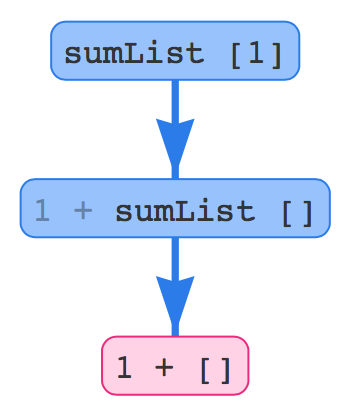
\includegraphics[height=1.5in]{nanomaly/sumList-overview.png}
\end{minipage}
\begin{minipage}{.49\linewidth}
\centering
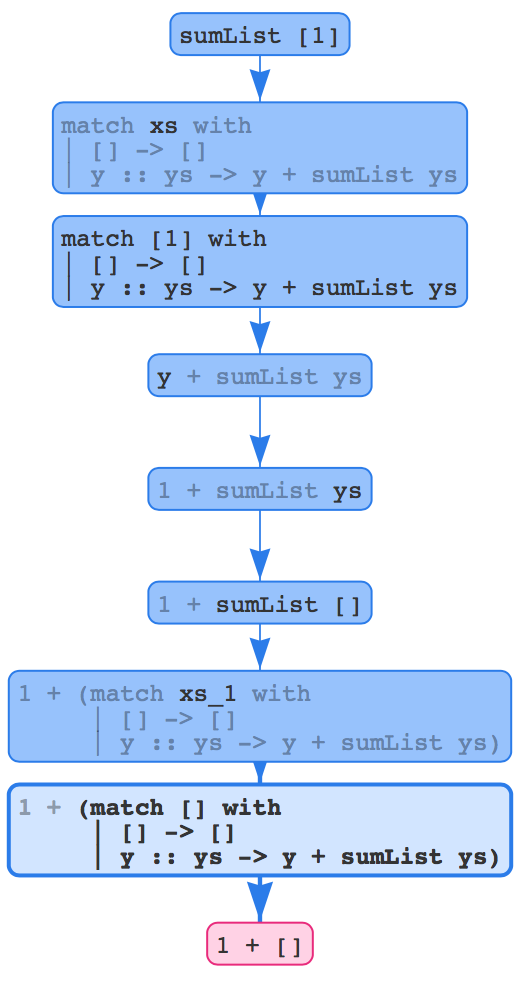
\includegraphics[height=3in]{nanomaly/sumList-long.png}
\end{minipage}
\vspace{1em}
\caption[(top-left) The ill-typed \texttt{sumList} function
  highlighting the error location reported by
  \ocaml. (bottom-left) Dynamically witnessing the type error in
  \texttt{sumList}, showing only function call-return pairs. (right) The
  same trace, fully expanded to show each small-step reduction in the
  computation.]{(top-left) The ill-typed \texttt{sumList} function
  \hlRed{highlighting} the error location reported by
  \ocaml. (bottom-left) Dynamically witnessing the type error in
  \texttt{sumList}, showing only function call-return pairs. (right) The
  same trace, fully expanded to show each small-step reduction in the
  computation.}
\label{fig:factorial}
\end{figure}

We have noticed a common theme in the existing literature on type error
diagnosis: errors are always presented in terms of the static type
system, and yet (static) type systems are meant to rule out certain
types of \emph{dynamic} errors.
%
We believe this may be particularly confusing for novice users, who must
simultaneously develop a mental model of the dynamic (evaluation)
semantics and the static (typing) semantics of the language they are
learning.
%
Furthermore, given the rise of dynamic languages like \textsc{Python}
and \textsc{Javascript} as teaching languages, novices may be more
familiar with reasoning about the dynamic semantics of a program than
the static semantics.
%
Thus, by connecting the static type error to the dynamic error it
would prevent, we might help novices understand the type system better.

In this chapter we propose a new approach that explains static type
errors by \emph{dynamically} witnessing how an ill-typed program goes
wrong.
%
We have developed \toolname, an interactive tool that uses
the source of the ill-typed function to automatically synthesize
the result on the bottom-left in Figure~\ref{fig:factorial}, which
shows how the recursive calls reduce to a configuration where
the program ``goes wrong'' --- \ie\ the @int@ value @0@ is to be
added to the @list@ value @[]@.
We achieve this via three concrete contributions.

\paragraph{1. Finding Witnesses}
Our first contribution is an algorithm for searching for
\emph{witnesses} to type errors, \ie\ inputs that cause a
program to go wrong~(\S~\ref{sec:nanomaly:searching-witness}).
%
This problem is tricky when we cannot rely on
static type information, as we must avoid the
trap of \emph{spurious} inputs that cause
irrelevant problems that would be avoided
by picking values of a different, relevant type.
%
We solve this problem by developing a novel
operational semantics that combines evaluation
and type inference.
%
We execute the program with \emph{holes} --- values whose type is
unknown --- as the inputs.
%
A hole remains abstract until the evaluation
context tells us what type it must have, for
example the parameters to an addition operation
must both be integers.
%
Our semantics conservatively instantiates holes
with concrete values, dynamically inferring the
type of the input until the program goes wrong.
%
We prove that our procedure synthesizes \emph{general}
witnesses, which means, intuitively, that if a witness
is found for a given ill-typed function, then, \emph{for all}
(inhabited) input types, there exist values that can make
the function go wrong.

Given a witness to a type error, the novice may still be at a loss.
%
The standard \ocaml\ interpreter and debugging infrastructure expect
well-typed programs, so they cannot be used to investigate \emph{how}
the witness causes the program to crash.
%
More importantly, the execution itself may be quite long and may contain
details not relevant to the actual error.

\paragraph{2. Visualizing Witnesses}
Our second contribution is an interactive visualization of the
execution of purely functional \ocaml\ programs, well-typed or not~(\S~\ref{sec:nanomaly:interactive}).
%
We extend the semantics to also build a \emph{reduction graph}
which records all of the small-step reductions and the context
in which they occur.
%
The graph lets us visualize the sequence of
steps from the source witness to the stuck term. The user can
interactively expand the computation to expose intermediate steps
by selecting an expression and choosing a traversal strategy.
%
The strategies include many of the standard debugging moves, \eg\
stepping \emph{forward} or \emph{into} or \emph{over} calls, as well
stepping or jumping \emph{backward} to understand how a particular
value was created, while preserving a context of the intermediate
steps that allow the user to keep track of a term's provenance.

We introduce a notion of \emph{jump-compressed} traces to abstract away
the irrelevant details of a computation.
%
A jump-compressed trace includes only function
calls and returns. For example, the trace in the bottom-left of
Figure~\ref{fig:factorial} is jump-compressed.
%
Jump-compressed traces are similar to stack traces in that both show a
sequence of function calls that lead to a crash. However, jump-compressed
traces also show the return values of successful calls, which can be
useful in understanding why a particular path was taken.

\paragraph{3. Evaluating Witnesses}
%
Of course, the problem of finding witnesses is
undecidable in general. In fact, due to the necessarily
conservative nature of static typing, there
may not even exist any witnesses for a given
ill-typed program.
%
Thus, our approach is a heuristic that is only useful
if it can find \emph{compact} witnesses for
\emph{real-world} programs.
%
Our third contribution is an extensive evaluation of our approach
on two different sets of ill-typed programs obtained by instrumenting
compilers used in beginner's classes~(\S~\ref{sec:nanomaly:evaluation}).
%
The first is the \uwbench\ dataset~\cite{Lerner2007-dt}, standard in the
literature, comprising \uwsize\ ill-typed programs.
%
The second comes from the new dataset described in \autoref{chp:data-collection}, comprising \ucsdsize\
ill-typed programs.
%
We show that for both datasets, our technique is able to generate
witnesses for around 85\% of the programs, in under a second in the
vast majority of cases.
%
Furthermore, we show that a simple interactive strategy yields
compact counterexample traces with at most 5 steps for 60\%
of the programs, and at most 10 steps for over 80\% of the programs.
%
We can even use witnesses to \emph{localize} type errors with a simple
heuristic that treats the values in a ``stuck'' term as \emph{sources}
of typing constraints and the term itself as a \emph{sink},
achieving around 70\% accuracy in locating the source of the error.

The ultimate purpose of an error report is to help the programmer
\emph{comprehend} and \emph{fix} problematic code.
%
Thus, our final contribution is a user study that compares \toolname's
dynamic witnesses against \ocaml's type errors along the dimension of
comprehensibility~(\S~\ref{sec:nanomaly:user-study}).
%
Our study finds that students given one of our witnesses are
consistently more likely to correctly explain and fix a type
error than those given the standard error message produced by
the \ocaml compiler.


%
% \subparagraph{Witness Utility}
%
% Even if we can find small witnesses for the majority of type errors, it
% may be that the witnesses do not actually help developers
% \emph{understand} the errors.
%
% In other words, perhaps the static error message is sufficient to
% diagnose and fix the error, or perhaps the witness simply does not add
% enough information to make a difference.
%
%
% Thus, our final contribution is a user study that compares the utility
% of our witnesses with that of the error messages provided by the \ocaml
% compiler~(\S~\ref{sec:nanomaly:user-study}).
%

\smallskip
All together, our results show that in the vast majority of cases, (novices') ill-typed
programs \emph{do} go wrong, and that the witnesses to these errors can be
helpful in understanding the source of the error. This, in turn, opens the
door to a novel dynamic way to explain, understand, and appreciate the
benefits of static typing.


%%% Local Variables:
%%% mode: latex
%%% TeX-master: "main"
%%% End:

\section{Overview}
\label{sec:overview}

We start with an overview of our approach to
explaining (static) type errors using \emph{witnesses}
that (dynamically) show how the program goes wrong.
%
We illustrate why generating suitable inputs
to functions is tricky in the absence of type
information.
%
Then we describe our solution to the problem
and highlight the similarity to static type
inference,
%
Finally, we demonstrate our visualization of
the synthesized witnesses.

\subsection{Generating Witnesses}
\label{sec:generating-witnesses}
Our goal is to find concrete values
that demonstrate how a program ``goes wrong''.

\paragraph{Problem: Which inputs are bad?}
%
One approach is to randomly generate input values and
use them to execute the program until we find one that
causes the program to go wrong.
%
Unfortunately, this approach quickly runs aground.
Recall the erroneous @fac@ function from Figure~\ref{fig:factorial}.
%~\S~\ref{sec:introduction}:
%
% \begin{code}
  % let rec fac n =
    % if n <= 0 then
      % true
    % else
      % n * fac (n-1)
% \end{code}
% \ES{having two copies of \texttt{fac} seems silly, but the back-reference across a page boundary is no good either...}
%
What \emph{types} of inputs should we test @fac@ with?
%
Values of type @int@ are fair game, but values of type, say,
@string@ or @int list@ will cause the program to go wrong
in an \emph{irrelevant} manner.
%
Concretely, we want to avoid testing @fac@ with any type other
than @int@ because any other type would cause @fac@ to get stuck
immediately in the @n <= 0@ test.

\paragraph{Solution: Don't generate inputs until forced.}
Our solution is to avoid generating a concrete value for the input at
all, until we can be sure of its type.
%
The intuition is that we want to be as lenient as possible in our tests,
so we make no assumptions about types until it becomes clear from the
context what type an input must have.
%
This is actually quite similar in spirit to type inference.

To defer input generation, we borrow the notion of a ``hole'' from
SmallCheck~\cite{Runciman2008-ka}.
%
A hole --- written \vhole{\thole} --- is a \emph{placeholder} for a
value \ehole of some unknown type \thole.
%
We leave all inputs as uninstantiated holes until they are demanded by
the program, \eg due to a primitive operation like the @<=@ test.

\paragraph{Narrowing Input Types}
Primitive operations, data construction, and case-analysis \emph{narrow}
the types of values.
%
For concrete values this amounts to a runtime type check, we ensure that
the value has a type compatible with the expected type.
%
For holes, this means we now know the type it should
have (or in the case of compound data we know \emph{more} about the
type) so we can instantiate the hole with a value.
%
The value may itself contain more holes, corresponding to components
whose type we still do not know.
%
Consider the @fst@ function:
%
\begin{code}
  let fst p = match p with
    (a, b) -> a
\end{code}
%
The case analysis tells us that @p@ must be a pair, but it says
\emph{nothing} about the contents of the pair.
%
Thus, upon reaching the case-analysis we would generate a pair
containing fresh holes for the @fst@ and @snd@ component.
%
Notice the similarity between instantiation of type variables and
instantiation of holes.
%
We can compute an approximate type for @fst@ by approximating the types
of the (instantiated) input and output, which would give us:
%
\begin{mcode}
  fst : ($\thole_1$ * $\thole_2$) -> $\thole_1$
\end{mcode}
%
We call this type approximate because we only see a single path through
the program, and thus will miss narrowing points that only occur in
other paths.

Returning to @fac@, given a hole as input we will narrow the hole
to an @int@ upon reaching the @<=@ test.
%
At this point we choose a
random @int@\footnote{With standard heuristics~\cite{Claessen2000-lj} to favor small values.}
for the instantiation and
concrete execution takes over entirely, leading us to the expected crash
in the multiplication.

\paragraph{Witness Generality}
We show in \S~\ref{sec:soundness} that our lazy instantiation of holes
produces \emph{general witnesses}.
%
That is, we show that if ``executing''
a function with a hole as input causes the
function to ``go wrong'', then there is
\emph{no possible} type for the function.
%
In other words, for \emph{any} types you might
assign to the function's inputs, there exist values
that will cause the function to go wrong.

\paragraph{Problem: How many inputs does a function take?}
%
There is another wrinkle, though; how did we know
that @fac@ takes a single argument instead of two
(or none)?
%
It is clear, syntactically, that @fac@ takes \emph{at least} one
argument, but in a higher-order language with currying, syntax can be
deceiving.
%
Consider the following definition:
%
\begin{code}
  let incAllByOne = List.map (+ 1)
\end{code}
%
Is @incAllByOne@ a function?
%
If so, how many arguments does it take?
%
The \ocaml\ compiler deduces that @incAllByOne@ takes a single argument
because the \emph{type} of \hbox{@List.map@} says it takes two arguments, and it is
partially applied to @(+ 1)@.
%
As we are dealing with ill-typed programs we do not have the luxury of
typing information.

\paragraph{Solution: Search for saturated application.}
We solve this problem by deducing the number of arguments
via an iterative process. We add arguments one-by-one
until we reach a \emph{saturated} application, \ie\
until evaluating the application returns a value
other than a lambda.

\subsection{Visualizing Witnesses}
\label{sec:visual-witness}
We have described how to reliably find witnesses to type errors in \ocaml,
but this does not fully address our original goal --- to \emph{explain}
the errors.
%
Having identified an input vector that triggers a crash, a common next
step is to step through the program with a \emph{debugger} to observe
how the program evolves.
%
The existing debuggers and interpreters for \ocaml\ assume a type-correct
program, so unfortunately we cannot use them off-the-shelf.
%
Instead we extend our search for witnesses to produce an execution
trace.

\paragraph{Reduction Graph}
Our trace takes the form of a reduction graph, which records small-step
reductions in the context in which they occur.
%
% These graphs have two types of edges:
% %
% (1) ``steps-to'' edges that capture the small-step transition between
% two terms, and
% %
% (2) ``sub-term'' edges that capture the containment relation between two
% terms.
%
For example, evaluating the expression @1+2+3@ would produce the
graph in Figure~\ref{fig:simple-reduction-hi}.
%
\begin{figure}[t]
  \centering
  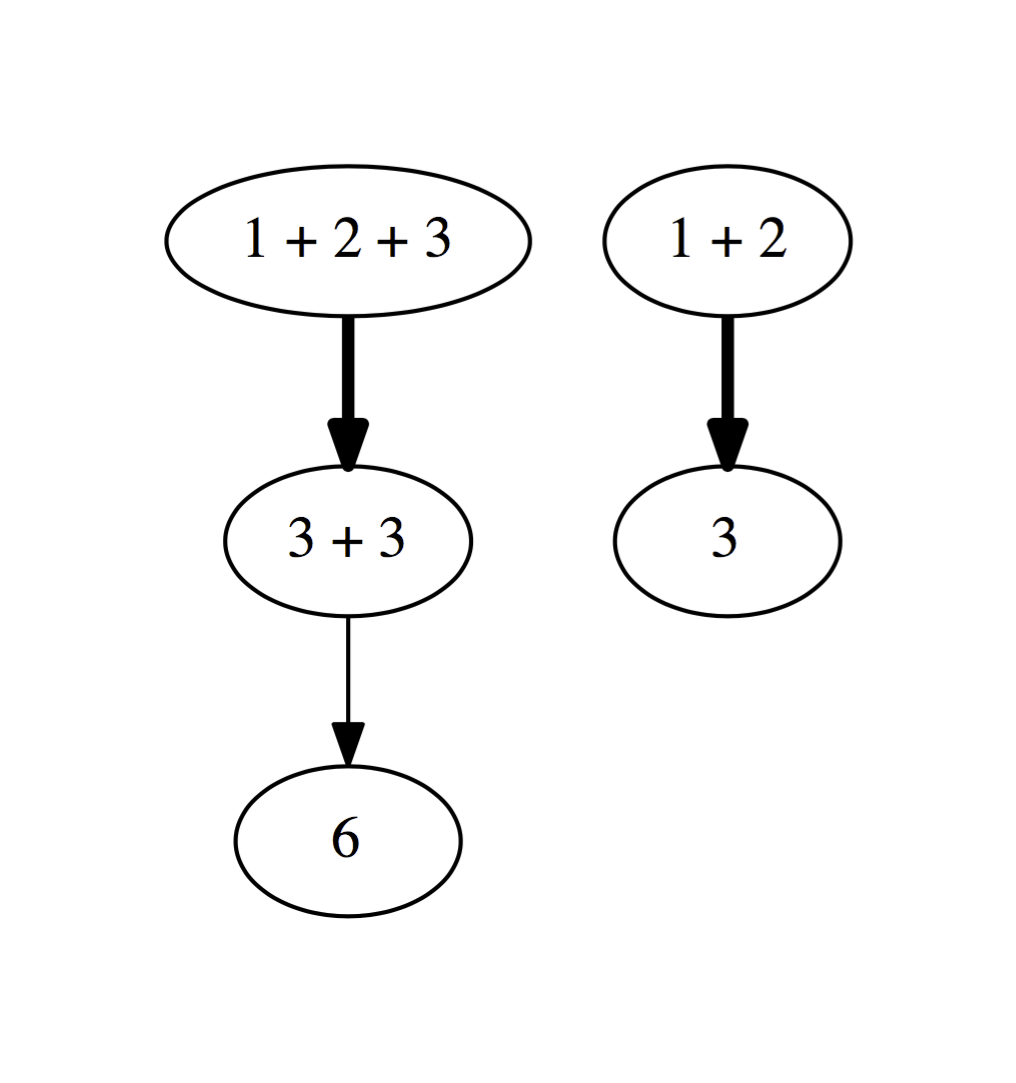
\includegraphics[height=2in]{nanomaly/simple.png}
  \caption{The reduction graph for \texttt{1+2+3}. The two edges
    produced by the transition from \texttt{1+2+3} to \hbox{\texttt{3+3}}
    are highlighted.}
\label{fig:simple-reduction-hi}
\end{figure}
%
Notice that when we transition from @1+2+3@ to @3+3@ we collect
both that edge \emph{and} an edge from the sub-term @1+2@ to @3@.
%
These additional edges allow us to implement two common debugging
operations \emph{post-hoc}: ``step into'' to zoom in on a specific
function call, and ``step over'' to skip over an uninteresting
sub-computation.

\paragraph{Interacting with the graph}
The reduction graph is useful for formulating and executing traversals,
but displaying it all at once would quickly become overwhelming.
%
Our interaction begins by displaying a big-step reduction, \ie the
witness followed by the stuck term.
%
The user can then progressively fill in the hidden steps of the
computation by selecting a visible term and choosing one of the
applicable traversal strategies --- described in
\S~\ref{sec:interactive} --- to insert another term into the
visualization.

\paragraph{Jump-compressed Witnesses}
It is rare for the initial state of the visualization to be
informative enough to diagnose the error.
%
Rather than abandon the user, we provide a short-cut to expand the witness
to a \emph{jump-compressed} trace, which contains every function call
and return step.
%
The jump-compressed trace abstracts the computation as a sequence of
call-response pairs, providing a high-level overview of steps taken
to reach the crash, and a high level of compression compared to the
full trace.
%
For example, the jump-compressed trace in Figure~\ref{fig:factorial}
contains 4 nodes compared to the 19 in the fully expanded trace.
%
Our benchmark suite of student programs shows that jump-compression is
practical, with an average jump-compressed trace size of 7 nodes and a
median of 5.

% A sample interaction with the trace of @fac 1@ can be seen in
% Figure~\ref{fig:nanomaly-factorial}.
% %
% % \begin{figure*}[t]
% % \centering
% % 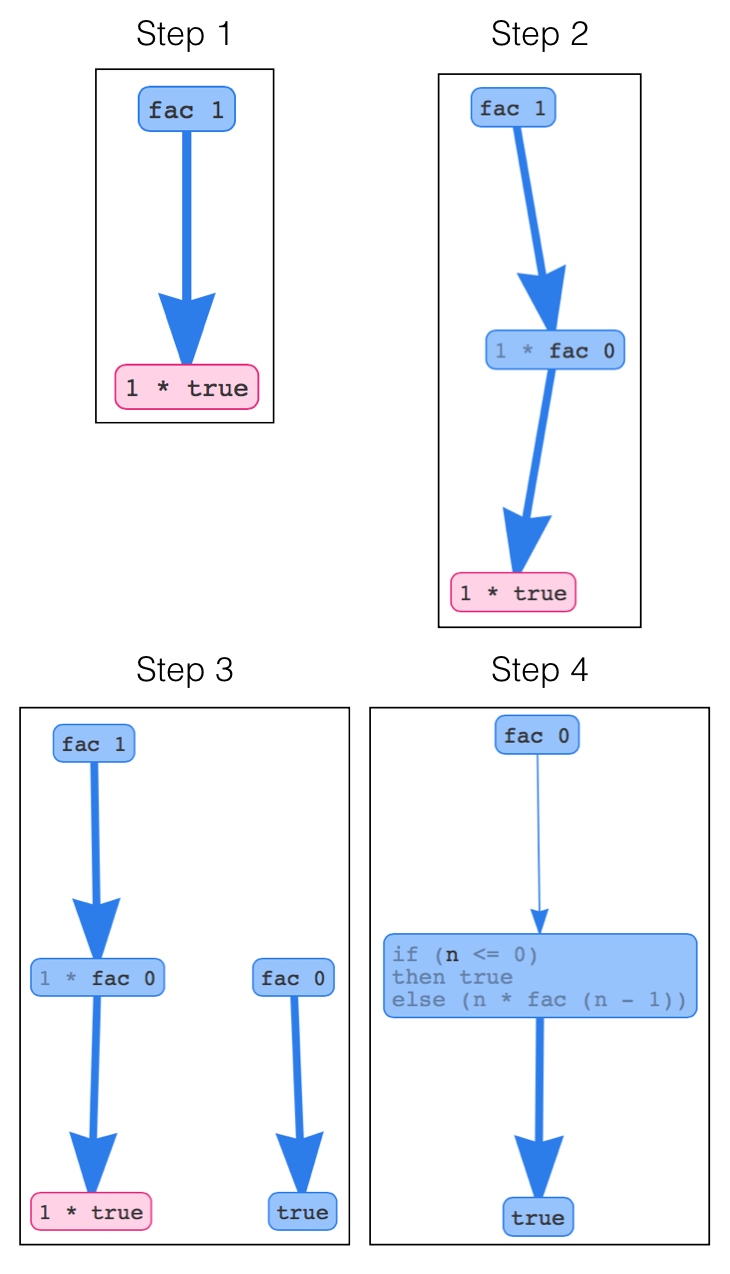
\includegraphics[width=0.8\linewidth]{fac-steps.png}
% % \caption{A sequence of interactions with the trace of
% %   \texttt{fac 1}. The stuck term is red, in each node the redex is
% %   highlighted. Thick arrows denote a multi-step transition, thin arrows
% %   denote a single-step transition. We start in step 1. In step 2 we jump
% %   forward from the witness to the next function call. In step 3 we step
% %   into the recursive \texttt{fac 0} call, which spawns a new ``thread''
% %   of execution. In step 4 we take a single step forward from
% %   \texttt{fac 0} (hiding the context for space).}
% % \label{fig:nanomaly-factorial}
% % \end{figure*}
% %
% The initial state of the visualization tells us that after some number
% of steps -- the thick arrow denotes a multi-step transition -- we try to
% multiply @1@ by @true@.

% Upon seeing the stuck term, we might wonder where @true@ came from.
% %
% To investigate we select the stuck term and click the ``jump backward''
% button to search backwards from the stuck term for the most recent
% function call, which brings us to @1 * fac 0@. Notice at this point that
% @fac 0@ is highlighted while @1 *@ is grayed out. This tells us that
% @fac 0@ is the redex in this term.

% @fac 0@ seems like the right thing to do so we choose to ``step into''
% it, which inserts a new multi-step transition from @fac 0@ to @true@.
% %
% Finally, we take a ``step forward'' from \hbox{@fac 0@,} bringing us to @fac@'s
% body. If we mouse over the body term we will see a popup with the
% environment at this point, notably telling us that @n = 0@. At this point
% it is clear that @fac@ handles the @n <= 0@ case incorrectly and should
% instead return an @int@.

% Upon seeing the stuck term, one might wonder where the @function@
% came from.
% %
% To investigate we select the stuck term and click the ``jump backward''
% button to search backwards from the stuck term for the most recent
% function call, which brings us to @listReverse [] = w@, in the same
% context as before.
% %
% Uncontent with the explanation so far, we ``step forward'' twice from
% the @listReverse []@ term, bringing us to @helper [] = w@.
% %
% At this point it is clear that the @helper@ function is not defined
% correctly, we have supplied it with the single argument we expected and
% yet it still returned a @function@.

% The problem is that the @function@ keyword in \ocaml defines an
% anonymous function that takes a single argument and immediately does a
% case-analysis without giving the argument a name.
% %
% The solution is to replace @function@ with an explicit @match xs with@
% -- naming the value we wish to case-analyse.
% %
% After applying our fix, \nanomaly -- and more importantly \ocaml --
% decide that @listReverse@ is safe to run.
% \ES{these last few paragraphs probably belong in the overview}
%





%%% Local Variables:
%%% mode: latex
%%% TeX-master: "main"
%%% End:

\section{Type-Error Witnesses}
\label{sec:nanomaly:searching-witness}

% Our goal is to find concrete values that demonstrate how a
% program ``goes wrong''.

% \paragraph{Problem: Which inputs are bad?}
% %
% One approach is to randomly generate input values and use
% them to execute the program until we find one that causes
% the program to go wrong. However, to see why this approach
% is naive, consider the following example:
% %
% \begin{lstlisting}
%   let f x =
%     let y = 1 + x in
%       1. +. y
% \end{lstlisting}
% %
% What \emph{types} of inputs should we test \texttt{f} with?
% Values of type \texttt{int} and \texttt{float} are fair game,
% but values of type say, \texttt{string} or \texttt{int list}
% will cause the program to go wrong in an \emph{irrelevant}
% manner.

% \paragraph{Solution:} \RJ{STOP}


% we cannot provide \emph{completely arbitrary} inputs to
% \texttt{f}. Instead, we call \texttt{f} with a \emph{hole}, written
% \ehole{}, which is a placeholder for a value whose type we have not
% yet determined. As we execute the program, we instantiate holes with
% concrete values as demanded by the primitive operations in the
% program. For example, the hole we pass to f will be instantiated to an
% int when we reach the \lstinline{1 + x} term. Thus, y will be an int as
% well, and the program will get stuck at \lstinline{1. +. y}. \ES{this
%   reads more like overview text..}
%


% \begin{itemize}
% \item how do we run ill-typed programs?
% \item for a lang like ocaml, dynamic semantics are independent of static
%   semantics, just lambda calculus. so no problem to run ill-typed
%   program
% \item but what about functions? what type of arguments should we pass? consider
%
% \begin{lstlisting}
% let f x =
%   let y = 1 + x in
%     1. +. y
% \end{lstlisting}
%
% does \texttt{f} take an int, float, string? int and float are both
% somewhat plausible, but string or anything else is ``clearly'' bogus. so
% we cannot provide \emph{completely arbitrary} inputs to
% \texttt{f}. Instead, we call \texttt{f} with a \emph{hole}, written
% \ehole{}, which is a placeholder for a value whose type we have not
% yet determined. As we execute the program, we instantiate holes with
% concrete values as demanded by the primitive operations in the
% program. For example, the hole we pass to f will be instantiated to an
% int when we reach the \lstinline{1 + x} term. Thus, y will be an int as
% well, and the program will get stuck at \lstinline{1. +. y}. \ES{this
%   reads more like overview text..}
%
% % \item values are tagged with their types, just like ``untyped'' langs
% % \item special ``hole'' value whose type is not yet known, used for function args
% % \item on-the-fly unification to determine ``correct'' type for holes
% \end{itemize}


Next, we formalize the notion of type error witnesses as follows.
%
First, we define a core calculus within which we will work~(\S~\ref{sec:nanomaly:syntax}).
%
Second, we develop a (non-deterministic) operational semantics
for ill-typed programs that precisely defines the notion
of a \emph{witness}~(\S~\ref{sec:nanomaly:semantics}).
%
Third, we formalize and prove a notion of \emph{generality} for
witnesses, which states, intuitively, that if we find a
single witness then for \emph{every possible} type
assignment there exist inputs that are guaranteed to make
the program ``go wrong''~(\S~\ref{sec:nanomaly:soundness}).
%
Finally, we refine the operational semantics into a
\emph{search procedure} that returns concrete (general)
witnesses for ill-typed programs~\S~(\ref{sec:nanomaly:search-algorithm}).
%
We have formalized and tested our semantics and generality theorem
in \textsc{PLT-Redex}~\cite{Felleisen2009-ya}.
%
Detailed proofs for the theorems in this section can be found in
%
\ifthenelse{\equal{\isTechReport}{true}}
{Appendix~\ref{sec:nanomaly:proofs}.}
{Appendix A of the accompanying tech report~\cite{Seidel2016Dynamic-TechRep}.}


\subsection{Syntax}
\label{sec:nanomaly:syntax}
\begin{figure}
% \hrule width 0.48\textwidth \vspace{0.05in}
$$
\begin{array}{rrcl}
% \emphbf{Configurations} \quad
%   & c & ::=    & \triple{e}{\vsu}{\tsu} \spmid \triple{\stuck}{\vsu}{\tsu} \\[0.05in]

\emphbf{Expressions}
  & \estuck & ::= & e \spmid \stuck \\
  & e & ::=    & v \spmid x \spmid \eapp{e}{e} \spmid \eplus{e}{e}\\
  &   & \spmid & \eif{e}{e}{e} \\
  % &   & \spmid & \elet{x}{e}{e} \\
  &   & \spmid & \epair{e}{e} \spmid \epcase{e}{x}{x}{e} \\
  % &   & \spmid & \einl{e} \spmid \einr{e} \spmid \escase{e}{x}{e}{x}{e}
  &   & \spmid & \econs{e}{e} \spmid \enil \\
  &   & \spmid & \elcase{e}{e}{x}{x}{e}
  % &   & \spmid & \enode{e}{e}{e} \spmid \eleaf \\
  % &   & \spmid & \ecase{e}{e}{x}{x}{x}{e}
\\[0.1in]

\emphbf{Values}
  & v  & ::= & n \spmid b \spmid \efun{x}{e} \spmid \vhole{\thole} \\
  &    & \spmid & \epair{v}{v} \spmid l \\
  % &    & \spmid & \vinl{t}{t}{v} \spmid \vinr{t}{t}{v}
  & l & ::= & \vcons{t}{v}{v} \spmid \vnil{t}
%  & tr & ::= & \vnode{t}{v}{v}{v} \spmid \vleaf{t}
\\[0.05in]

\emphbf{Integers}
  & n & ::= &  0,1,-1,\ldots \\[0.05in]

\emphbf{Booleans}
  & b & ::= &  \etrue \spmid \efalse \\[0.05in]

\emphbf{Types}
  & t & ::=     & \tbool \spmid \tint \spmid \tfun \\
  &   &  \spmid & \tprod{t}{t} \spmid \tlist{t} \spmid \thole \\[0.05in]

\emphbf{Substitutions}
  & \vsu & ::= & \{\nu_1^{\thole_1} \mapsto v_n, \ldots, \nu_n^{\thole_n} \mapsto v_n\} \\
  & \tsu & ::= & \{\thole_1 \mapsto t_n, \ldots, \thole_n \mapsto t_n\} \\[0.1in]
  % & \vsu & ::= & \emptysu \spmid \extendsu{\vsu}{\vhole{\thole}}{v} \\
  % & \tsu & ::= & \emptysu \spmid \extendsu{\tsu}{\thole}{t} \\[0.1in]
% \end{array}
% $$
% % \hrule width 0.48\textwidth
% $$
% \begin{array}{rrcl}
\emphbf{Contexts}
  & C
  & ::=
  &   	 \bullet
  \spmid \eapp{C}{e}
  \spmid \eapp{v}{C} \\
  & & \spmid & \eplus{C}{e} \spmid \eplus{v}{C} \\
  & & \spmid & \eif{C}{e}{e} \\
  % & & \spmid & \elet{x}{C}{e} \\
  & & \spmid & \epair{C}{e} \spmid \epair{v}{C} \\
  & & \spmid & \epcase{C}{x}{x}{e} \\
  % & & \spmid & \einl{C} \spmid \einr{C} \\
  % & & \spmid & \escase{C}{x}{e}{x}{e}
  & & \spmid & \econs{C}{e} \spmid \econs{v}{C} \\
  & & \spmid & \elcase{C}{e}{x}{x}{e}

  % & & \spmid & \enode{C}{e}{e} \spmid \enode{v}{C}{e} \spmid \enode{v}{v}{C} \\
  % & & \spmid & \ecase{C}{e}{x}{x}{x}{e}
\\[0.05in]
\end{array}
$$

% \judgementHead{Reduction}{\eval{e}{e}}

% $$
% \begin{array}{rcl}
% \eval{C[e]&}{&C[e']} \qquad \text{if}\ \eval{e}{e'} \\
% 	\eval{\eapp{c}{v}&}{& \ceval{c}{v}}\\
% \eval{\eapp{(\efun{x}{\tau_x}{e})}{e_x}&}{&e\sub{x}{e_x}}\\
% 	\eval{\elet{x}{e_x}{e}&}{&e\sub{x}{e_x}} \\
% 	\eval{\ecase{D_j\ \overline{e}}{D_i}{\overline{y_i}}{e_i}{x}&}
% 	{&e_j\sub{x}{D_j\ \overline{e}}\sub{\overline{y_j}}{\overline{e}}} \\
% \end{array}
% $$

\caption{Syntax of \lang}
\label{fig:syntax}
\end{figure}

%
Figure~\ref{fig:syntax} describes the syntax of \lang, a simple lambda
calculus with integers, booleans, pairs, and lists.
%
As we are specifically interested in programs that \emph{do} go wrong,
we include an explicit \stuck\ term in our syntax. We write $\estuck$ to
denote terms that may be \stuck, and $e$ to denote terms that may not be
stuck.

\paragraph{Holes}
\label{sec:nanomaly:holes}
%
Recall that a key challenge in our setting is to find witnesses
that are meaningful and do not arise from choosing values from
irrelevant types.
%
We solve this problem by equipping our term language with a
notion of a \emph{hole}, written \vhole{\thole}, which represents
an \emph{unconstrained} value $\ehole$ that may be replaced with
\emph{any} value of an unknown type \thole.
%
Intuitively, the type holes \thole\ can be viewed as type variables
that we will \emph{not} generalize over.
%
A \emph{normalized} value is one that is not a hole,
but which may internally contain holes.
%
For example
$\epair{\ehole_1[\thole_1]}{\ehole_2[\thole_2]}$
% $\vnode{\thole}{\vhole{\thole}}{\vleaf{\thole}}{\vleaf{\thole}}$
is a normalized value.

\paragraph{Substitutions}
%
Our semantics ensure the generality of witnesses by incrementally
\emph{refining} holes, filling in just as much information as is
needed locally to make progress (inspired by the manner in
which SmallCheck uses lazy evaluation~\cite{Runciman2008-ka}).
%
We track how the holes are incrementally filled in, by using
value (resp.\ type) \emph{substitutions} $\vsu$ (resp. $\tsu$)
that map value (resp.\ type) holes to values (resp.\ types).
%
The substitutions let us ensure that we consistently instantiate each
hole with the same (partially defined) value or type, regardless of the
multiple contexts in which the hole appears.
%
This ensures we can report a concrete (and general) witness for any
(dynamically) discovered type errors.

A \emph{normalized} value substitution is one whose co-domain is
comprised of normalized values.
%
In the sequel, we will assume and ensure that all value substitutions
are normalized.
%
We ensure additionally that the co-domain of a substitution does not
refer to any elements of its domain, \ie when we extend a substitution
with a new binding we apply the substitution to itself.
%
We will use the notation $\extendsu{\tsu}{\thole}{t}$ for the extension
of a type (\resp value) substitution, to distinguish it from a simple
set union.

% \paragraph{Resolving Holes}
% We \emph{resolve} a hole with respect to a substitution by
% transitively applying the substitution as long as it contains
% any holes that are defined in the substitution.
% %
% We write \resolve{\thole}{\tsu} to denote the the resolution
% of \thole\ with respect to \tsu.
% %
% Note that by definition, \resolve{\thole}{\tsu} does not contain
% any holes in the domain of \tsu.


\subsection{Semantics}
\label{sec:nanomaly:semantics}
%
Recall that our goal is to synthesize a value that demonstrates
why (and how) a function goes wrong.
%
We accomplish this by combining evaluation with type inference,
giving us a form of dynamic type inference.
% starting with an unconstrained hole and gradually refining it
% as evaluation constrains its type.
%
Each primitive evaluation step tells us more about the types of the
program values. For example, addition tells us that the addends must be
integers, and % case-analysis tells us that the scrutinee must be a tree.
an if-expression tells us the condition must be a boolean.
%
When a hole appears in such a context, we know what type it must have
in order to make progress and can fill it in with a concrete value.

The evaluation relation is parameterized by a pair of functions,
\emph{narrow} (\forcesym) and \emph{generate} (\gensym),
that ``dynamically'' perform type-checking and hole-filling
respectively.

\paragraph{Narrowing Types}
The procedure % $\force{v}{t}{\vsu}{\tsu}$,
\[
\forcesym : v \times t \times \vsu \times \tsu \rightarrow \triple{v \cup \stuck}{\vsu}{\tsu}
\]%
defined in Figure~\ref{fig:narrow}, takes as input a value $v$, a type
$t$, and the current value and type substitutions, and refines $v$ to
have type $t$ by yielding a triple of either the same value and
substitutions, or yields the stuck state if no such refinement is
possible. In the case where $v$ is a hole, it first checks in the given
$\vsu$ to see if the hole has already been instantiated and, if so,
returns the existing instantiation.
%
For convenience, \forcesym uses a variant of Robinson's \U~\citep{Robinson1965-rk} that unifies
a set of types, and that takes and updates an existing substitution.
%
\begin{figure}[t]
\[
\boxed{
\begin{array}{lll}
%% \multicolumn{3}{l}{\forcesym \ :: \  (e, t) \rightarrow \pair{e}{\vsu}} \\
\forcesym                  & : v \times t \times \vsu \times \tsu \rightarrow \triple{v \cup \stuck}{\vsu}{\tsu} \\[0.1in]
% \force{v}{\thole}{\vsu}{\tsu}  & \defeq & \hspace{-1ex}
% \begin{cases}
%   \triple{v}{\vsu}{\tsu'} & \mbox{if } \tsu' = \unify{\{\typeof{v}, \thole\}}{\tsu} \\
%   \triple{\stuck}{\vsu}{\tsu} & \mbox{otherwise} \\

%   % \force{v}{\subst{\tsu}{\thole}}{\vsu}{\tsu} & \mbox{if}\ \thole \in dom(\tsu) \\
%   % \triple{v}{\vsu}{\extendsu{\tsu}{\thole}{\typeof{v}}} & \mbox{otherwise} \\
% \end{cases} \\
\force{\vhole{\thole}}{t}{\vsu}{\tsu} & \defeq % \hspace{-1ex}
\begin{cases}
  \triple{v}{\vsu}{\tsu'}    &\ \textbf{if} \begin{array}{l} v = \lookupsu{\vsu}{\vhole{\thole}}, \\
                                         \tsu' = \unify{\{\thole, t, \typeof{v}\}}{\tsu}\end{array} \\
  \triple{\stuck}{\vsu}{\tsu} &\ \textbf{if} \begin{array}{l} v = \lookupsu{\vsu}{\vhole{\thole}}\end{array} \\
  \triple{v}{\extendsu{\vsu}{\vhole{\thole}}{v}}{\tsu'} &\ \textbf{if} \begin{array}{l} \tsu' = \unify{\{\thole, t\}}{\tsu}, \\ v = \gen{t}{\tsu'} \end{array}\\
\end{cases}  \\[0.05in]
% \begin{cases}
%   \triple{\lookupsu{\vsu}{\ehole}}{\vsu}{\tsu} & \mbox{if}\ \ehole \in dom(\vsu), \hastype{\lookupsu{\vsu}{\ehole}}{t} \\
%   \triple{\stuck}{\vsu}{\tsu}                  & \mbox{if}\ \ehole \in dom(\vsu) \\
%   \triple{v}{\extendsu{\vsu}{\ehole}{v}}{\tsu}   & v = \gen{t}\\
% \end{cases} \\
 % \begin{array}{l}
    % \mathtt{if}\ i \in \vsu\ \mathtt{then}\ \triple{\vsu(i)}{\vsu}\ \mathtt{else} \\
         % \elet{v}{\gen{t}}{\triple{v}{\ehole{i} \mapsto v}}
  % \end{array} \\
\force{n}{\tint}{\vsu}{\tsu}     & \defeq \triple{n}{\vsu}{\tsu} \\[0.05in]
\force{b}{\tbool}{\vsu}{\tsu}    & \defeq \triple{b}{\vsu}{\tsu} \\[0.05in]
\force{\efun{x}{e}}{\tfun}{\vsu}{\tsu} & \defeq \triple{\efun{x}{e}}{\vsu}{\tsu} \\[0.05in]
\force{\epair{v_1}{v_2}}{\tprod{t_1}{t_2}}{\vsu}{\tsu} & \defeq \triple{\epair{v_1}{v_2}}{\vsu}{\tsu''} \hspace{0.66in} \textbf{if} \begin{array}{l} \tsu' = \unify{\{\typeof{v_1}, t_1\}}{\tsu},\\ \tsu'' = \unify{\{\typeof{v_2}, t_2\}}{\tsu'} \end{array} \\[0.05in]
% \force{\einl{v}}{\tsum{t_1}{t_2}}{\vsu}{\tsu} & \defeq \triple{\vinl{t_1}{t_2}{v}}{\vsu}{\tsu'} \hspace{0.53in} \textbf{if } \tsu' = \unify{\{\typeof{v}, t_1\}}{\tsu} \\
% \force{\einr{v}}{\tsum{t_1}{t_2}}{\vsu}{\tsu} & \defeq \triple{\vinr{t_1}{t_2}{v}}{\vsu}{\tsu'} \hspace{0.53in} \textbf{if } \tsu' = \unify{\{\typeof{v}, t_2\}}{\tsu} \\
% \force{\vleaf{t_1}}{\ttree{t_2}}{\vsu}{\tsu} & \defeq \triple{\vleaf{t_1}}{\vsu}{\tsu'} & \hspace{-43.5mm} \textbf{if} \begin{array}{l} \tsu' = \unify{\{t_1, t_2\}}{\tsu} \end{array}\\
% \force{\vnode{t_1}{v_1}{v_2}{v_3}}{\ttree{t_2}}{\vsu}{\tsu} \hspace{-3mm} & \defeq \triple{\vnode{t_1}{v_1}{v_2}{v_3}}{\vsu}{\tsu'} & \hspace{-43.5mm} \textbf{if} \begin{array}{l} \tsu' = \unify{\{t_1, t_2\}}{\tsu} \end{array} \\
\force{\vnil{t_1}}{\tlist{t_2}}{\vsu}{\tsu} & \defeq \triple{\vnil{t_1}}{\vsu}{\tsu'} \hspace{0.96in} \textbf{if} \begin{array}{l} \tsu' = \unify{\{t_1, t_2\}}{\tsu} \end{array}\\[0.05in]
\force{\vcons{t_1}{v_1}{v_2}}{\tlist{t_2}}{\vsu}{\tsu} \hspace{-3mm} & \defeq \triple{\vcons{t_1}{v_1}{v_2}}{\vsu}{\tsu'} \hspace{0.64in} \textbf{if} \begin{array}{l} \tsu' = \unify{\{t_1, t_2\}}{\tsu} \end{array} \\[0.05in]
\force{v}{t}{\vsu}{\tsu} & \defeq \triple{\stuck}{\vsu}{\tsu}
\end{array}
}
\]
\caption{Narrowing values}
\label{fig:narrow}
\end{figure}
%
%While a hole may map to a value that \emph{contains} another hole, \eg a
%lambda or a tree, it may not map \emph{directly} to another hole,
As the value substitution is normalized, in the first case of \forcesym\ we
do not need to \forcesym\ the result of the substitution, the sub-hole
will be narrowed when the context demands it.

\paragraph{Generating Values} The (non-deterministic)
$\gen{t}{\tsu}$ in Figure~\ref{fig:gen} takes
as input a type $t$ and returns a value of that type.
%
For base types the procedure returns an arbitrary value of
that type.
%
For functions it returns a lambda with a \emph{new} hole
denoting the return value.
%
For unconstrained types (denoted
by $\thole$) it yields a fresh hole constrained to have type
\thole (denoted by $\vhole{\thole}$).
%
When generating a $\tlist{t}$ we must take care to ensure
the resulting tree is well-typed.
% %
For a polymorphic type $\tlist{\thole}$ %, eg in \recasegoodone,
or $\tprod{\thole_1}{\thole_2}$
we will place holes in the generated value; they will be lazily filled
in later, on demand.


\begin{figure}[t]
\[
\boxed{
\begin{array}{lcll}
\gensym       & :   & t \times \tsu \rightarrow v \\
\gen{\thole}{\tsu}  & \defeq  & \gen{\subst{\tsu}{\thole}}{\tsu} &  \text{if } \thole \in dom(\tsu) \\
\gen{\tint}{\tsu}   & \defeq  & n &  \text{non-det.} \\
\gen{\tbool}{\tsu}  & \defeq  & b &  \text{non-det.} \\
\gen{\tprod{t_1}{t_2}}{\tsu}  & \defeq  & \epair{\gen{t_1}{\tsu}}{\gen{t_2}{\tsu}} & \\ % \begin{subarray}{l} v_1 = \gen{t_1}{\tsu}\\ v_2 = \gen{t_2}{\tsu}\end{subarray} \\
% \gen{\ttree{t}}{\tsu}  & \defeq  & tr &  \text{non-det.} \\
\gen{\tlist{t}}{\tsu}  & \defeq  & l &  \text{non-det.} \\
% \gen{\tsum{t_1}{t_2}}{\tsu}  & \defeq  & \vinl{t_1}{t_2}{\gen{t_1}{\tsu}}\ \mathbf{or}\ \vinr{t_1}{t_2}{\gen{t_2}{\tsu}} & \text{non-det.} \\
\gen{\tfun}{\tsu}   & \defeq & \efun{x}{\vhole{\thole}} &  \text{\ehole, \thole are fresh} \\
\gen{\thole}{\tsu}  & \defeq & \vhole{\thole} & \text{\ehole is fresh} \\
\end{array}
}
\]
\caption{Generating values}
\label{fig:gen}
\end{figure}


\paragraph{Steps and Traces}
\begin{figure}[p]
%\begin{adjustbox}{center}
\begin{framed}
\judgementHead{Evaluation}{\step{\estuck}{\vsu}{\tsu}{\estuck}{\vsu}{\tsu}}
\small
\begin{gather*}
% \inference[\recontext]
%   {\step{e}{\su}{e'}{\su'}}
%   {\step{C[e]}{\su}{C[e']}{\su'}}
% \qquad
% \inference[\restuck]
%   {}
%   {\step{C[\stuck]}{\su}{\stuck}{\su}}
% \\ \\
% \inference[\reholegood]
%   {\thole \mbox{ is fresh}}
%   {\step{\ehole}{\vsu}{\tsu}{\vhole{\thole}}{\vsu}{\tsu}}
% \\ \\
\inference[\replusgood]
  {\triple{n_1}{\vsu'}{\tsu'} = \force{v_1}{\tint}{\vsu}{\tsu} \\
   \triple{n_2}{\vsu''}{\tsu''} = \force{v_2}{\tint}{\vsu'}{\tsu'} \\
   n = \eplus{n_1}{n_2}}
  {\step{\inctx{\eplus{v_1}{v_2}}}{\vsu}{\tsu}{\inctx{n}}{\vsu''}{\tsu''}}
\\[0.1in]
\inference[\replusbadone]
  {\triple{\stuck}{\vsu'}{\tsu'} = \force{v_1}{\tint}{\vsu}{\tsu}}
  {\step{\inctx{\eplus{v_1}{v_2}}}{\vsu}{\tsu}{\stuck}{\vsu'}{\tsu'}}
\\[0.1in]
\inference[\replusbadtwo]
  {\triple{\stuck}{\vsu'}{\tsu'} = \force{v_2}{\tint}{\vsu}{\tsu}}
  {\step{\inctx{\eplus{v_1}{v_2}}}{\vsu}{\tsu}{\stuck}{\vsu'}{\tsu'}}
\\[0.2in]
\inference[\reifgoodone]
  {\triple{\etrue}{\vsu'}{\tsu'} = \force{v}{\tbool}{\vsu}{\tsu}}
  {\step{\inctx{\eif{v}{e_1}{e_2}}}{\vsu}{\tsu}{\inctx{e_1}}{\vsu'}{\tsu'}}
\\[0.1in]
\inference[\reifgoodtwo]
  {\triple{\efalse}{\vsu'}{\tsu'} = \force{v}{\tbool}{\vsu}{\tsu}}
  {\step{\inctx{\eif{v}{e_1}{e_2}}}{\vsu}{\tsu}{\inctx{e_2}}{\vsu'}{\tsu'}}
\\[0.1in]
\inference[\reifbad]
  {\triple{\stuck}{\vsu'}{\tsu'} = \force{v}{\tbool}{\vsu}{\tsu}}
  {\step{\inctx{\eif{v}{e_1}{e_2}}}{\vsu}{\tsu}{\stuck}{\vsu'}{\tsu'}}
\\[0.2in]
\inference[\reappgood]
  {\triple{\efun{x}{e}}{\vsu'}{\tsu'} = \force{v_1}{\tfun}{\vsu}{\tsu}}
  {\step{\inctx{\eapp{v_1}{v_2}}}{\vsu}{\tsu}{\inctx{e\sub{x}{v_2}}}{\vsu'}{\tsu'}}
\\[0.1in]
\inference[\reappbad]
  {\triple{\stuck}{\vsu'}{\tsu'} = \force{v_1}{\tfun}{\vsu}{\tsu}}
  {\step{\inctx{\eapp{v_1}{v_2}}}{\vsu}{\tsu}{\stuck}{\vsu'}{\tsu'}}
\\[0.2in]
\inference[\repcasegood]
  {\thole_1, \thole_2 \mbox{ are fresh} & \triple{\epair{v_1}{v_2}}{\vsu_1}{\tsu_1} = \force{v}{\tprod{\thole_1}{\thole_2}}{\vsu}{\tsu}
  }
  {\step{\inctx{\epcase{v}{x_1}{x_2}{e}}}{\vsu}{\tsu}
        {\inctx{e\sub{x_1}{v_1}\sub{x_2}{v_2}}}{\vsu_1}{\tsu_1}}
\\[0.1in]
\inference[\repcasebad]
  {\thole_1, \thole_2 \mbox{ are fresh} & \triple{\stuck}{\vsu_1}{\tsu_1} = \force{v}{\tprod{\thole_1}{\thole_2}}{\vsu}{\tsu}
  }
  {\step{\inctx{\epcase{v}{x_1}{x_2}{e}}}{\vsu}{\tsu}
        {\stuck}{\vsu_1}{\tsu_1}}
%\\[0.2in]
\end{gather*}
\end{framed}
%\captionsetup{labelformat=empty}
\caption{Evaluation relation for \lang}
\end{figure}
\begin{figure}[p]
\ContinuedFloat
\captionsetup{list=off}
\begin{framed}
\judgementHead{Evaluation (\textit{ctd.})}{\step{\estuck}{\vsu}{\tsu}{\estuck}{\vsu}{\tsu}}
\small
\begin{gather*}
% \inference[\reinlgood]
%   {\thole \mbox{ is fresh}}
%   {\step{\inctx{\einl{v}}}{\vsu}{\tsu}{\inctx{\vinl{\typeof{v}}{\thole}{v}}}{\vsu}{\tsu}}
% \\[0.1in]
% \inference[\reinrgood]
%   {\thole \mbox{ is fresh}}
%   {\step{\inctx{\einr{v}}}{\vsu}{\tsu}{\inctx{\vinr{\thole}{\typeof{v}}{v}}}{\vsu}{\tsu}}
% \\[0.2in]
% \inference[\rescasegoodone]
%   {\thole_1, \thole_2 \mbox{ are fresh} & \triple{\vinl{t_1}{t_2}{v_1}}{\vsu_1}{\tsu_1} = \force{v}{\tsum{\thole_1}{\thole_2}}{\vsu}{\tsu}
%   }
%   {\step{\inctx{\escase{v}{x}{e_1}{x}{e_2}}}{\vsu}{\tsu}
%         {\inctx{e_1\sub{x}{v_1}}}{\vsu_1}{\tsu_1}}
% \\[0.1in]
% \inference[\rescasegoodtwo]
%   {\thole_1, \thole_2 \mbox{ are fresh} & \triple{\vinr{t_1}{t_2}{v_1}}{\vsu_1}{\tsu_1} = \force{v}{\tsum{\thole_1}{\thole_2}}{\vsu}{\tsu}
%   }
%   {\step{\inctx{\escase{v}{x}{e_1}{x}{e_2}}}{\vsu}{\tsu}
%         {\inctx{e_2\sub{x}{v_1}}}{\vsu_1}{\tsu_1}}
% \\[0.1in]
% \inference[\rescasebad]
%   {\thole_1, \thole_2 \mbox{ are fresh} & \triple{\stuck}{\vsu_1}{\tsu_1} = \force{v}{\tsum{\thole_1}{\thole_2}}{\vsu}{\tsu}
%   }
%   {\step{\inctx{\escase{v}{x}{e_1}{x}{e_2}}}{\vsu}{\tsu}
%         {\stuck}{\vsu_1}{\tsu_1}}
% \\[0.2in]
\inference[\renilgood]
  {\thole \mbox{ is fresh}}
  {\step{\inctx{\enil}}{\vsu}{\tsu}{\inctx{\vnil{\thole}}}{\vsu}{\tsu}}
\\[0.2in]
% \ES{what about $\tsu = unify(\thole, \typeof{v_1}, \typeof{v_2}, \typeof{v_3})$, then narrow to $\subst{\tsu}{\thole}$}
\inference[\reconsgood]
  {
   % \thole \mbox{ is fresh} \\
   % \triple{v_1'}{\vsu_1}{\tsu_1} = \force{v_1}{\thole}{\vsu}{\tsu} \\
   % \triple{v_2'}{\vsu_2}{\tsu_2} = \force{v_2}{\ttree{\thole}}{\vsu_1}{\tsu_1} \\
   % \triple{v_3'}{\vsu_3}{\tsu_3} = \force{v_3}{\ttree{\thole}}{\vsu_2}{\tsu_2} \\
   t = \typeof{v_1} \\
   \triple{v_2'}{\vsu_2}{\tsu_2} = \force{v_2}{\tlist{t}}{\vsu_1}{\tsu_1} \\
  % \triple{v_3'}{\vsu_3}{\tsu_3} = \force{v_3}{\ttree{t}}{\vsu_2}{\tsu_2} \\
  }
  {\step{\inctx{\econs{v_1}{v_2}}}{\vsu}{\tsu}
        {\inctx{\vcons{t}{v_1}{v_2'}}}{\vsu_2}{\tsu_2}}
\\[0.1in]
\inference[\reconsbad]
  {
   % \thole \mbox{ is fresh} \\
   % \triple{v_1'}{\vsu_1}{\tsu_1}   = \force{v_1}{\thole}{\vsu}{\tsu} \\
   t = \typeof{v_1} \\
   \triple{\stuck}{\vsu_2}{\tsu_2} = \force{v_2}{\tlist{t}}{\vsu_1}{\tsu_1} \\
  }
  {\step{\inctx{\econs{v_1}{v_2}}}{\vsu}{\tsu}
        {\stuck}{\vsu_2}{\tsu_2}}
% \\[0.1in]
% \inference[\renodebadtwo]
%   {
%    % \thole \mbox{ is fresh} \\
%    % \triple{v_1'}{\vsu_1}{\tsu_1} = \force{v_1}{\thole}{\vsu}{\tsu} \\
%    t = \typeof{v_1} \\
%    \triple{v_2'}{\vsu_2}{\tsu_2} = \force{v_2}{\ttree{t}}{\vsu_1}{\tsu_1} \\
%    \triple{\stuck}{\vsu_3}{\tsu_3} = \force{v_3}{\ttree{t}}{\vsu_2}{\tsu_2} \\
%   }
%   {\step{\inctx{\enode{v_1}{v_2}{v_3}}}{\vsu}{\tsu}
%         {\stuck}{\vsu_3}{\tsu_3}}
\\[0.2in]
\inference[\recasegoodone]
  {\thole \mbox{ is fresh} & \triple{\vnil{t}}{\vsu_1}{\tsu_1} = \force{v}{\tlist{\thole}}{\vsu}{\tsu}
  }
  {\step{\inctx{\elcase{v}{e_1}{x_1}{x_2}{e_2}}}{\vsu}{\tsu}
        {\inctx{e_1}}{\vsu_1}{\tsu_1}}
\\[0.1in]
\inference[\recasegoodtwo]
  {\thole \mbox{ is fresh} & \triple{\vcons{t}{v_1}{v_2}}{\vsu_1}{\tsu_1} = \force{v_1}{\tlist{\thole}}{\vsu}{\tsu}
  }
  {\step{\inctx{\elcase{v}{e_1}{x_1}{x_2}{e_2}}}{\vsu}{\tsu}
        {\inctx{e_2\sub{x_1}{v_1}\sub{x_2}{v_2}}}{\vsu_1}{\tsu_1}}
\\[0.1in]
\inference[\recasebad]
  {\thole \mbox{ is fresh} & \triple{\stuck}{\vsu_1}{\tsu_1} = \force{v}{\tlist{\thole}}{\vsu}{\tsu}
  }
  {\step{\inctx{\elcase{v}{e_1}{x_1}{x_2}{e_2}}}{\vsu}{\tsu}
        {\stuck}{\vsu_1}{\tsu_1}}
%\\[0.2in]
% \inference[\relet]
%   {v' = \generalize{v}{\tsu}}
%   {\step{\inctx{\elet{x}{v}{e}}}{\vsu}{\tsu}
%         {\inctx{e\sub{x}{v'}}}{\vsu}{\tsu}}
\end{gather*}
\end{framed}
%\end{adjustbox}
%\\ % [0.05in]
%% \relDescription{\forcesym and \gensym}
%% \begin{gather*}
%% \begin{array}{lcl}
%% \force{\ehole{i}}{t} & \defeq & \elet{v}{\gen{t}}{\pair{v}{\ehole{i} \mapsto v}} \\
%% \force{v}{\ehole{}}  & \defeq & \pair{v}{\emptysu} \\
%% \force{n}{\tint}    & \defeq & \pair{n}{\emptysu} \\
%% \force{v}{\tint}    & \defeq & \pair{\stuck}{\emptysu} \\
%% \force{b}{\tbool}   & \defeq & \pair{b}{\emptysu} \\
%% \force{v}{\tbool}   & \defeq & \pair{\stuck}{\emptysu} \\
%% \force{\efun{x}{e}}{\tfun{\thole{}}{\thole{}}} & \defeq & \pair{\efun{x}{e}}{\emptysu} \\
%% \force{v}{\tfun{\thole{}}{\thole{}}} & \defeq & \pair{\stuck}{\emptysu} \\
%% \end{array}
%% \qquad
%% \begin{array}{lcll}
%% \gen{\tint}   & \defeq & n & \\
%% \gen{\tbool}  & \defeq & b & \\
%% \gen{\tfun{t_1}{t_2}} & \defeq & \efun{x}{\ehole{i}}, & \quad \text{$i$ is fresh} \\
%% \gen{\thole{}} & \defeq & \ehole{i}, & \quad \text{$i$ is fresh} \\
%% \end{array}
%% \end{gather*}
\caption{Evaluation relation for \lang (\textit{ctd.})}
\label{fig:operational}
\end{figure}

%
% WRW notes that Figure 4 does not seem to handle recursion (it's not clear
% how the let rule would work for something "let rec"-y, and there's not
% function call rule). I only mention this because I can imagine a reviewer
% wondering about your ability to generate good witnesses for function
% types. This could likely be addressed in text, by a forward reference to
% Section 3.4 where higher-order functions are handled, without changing
% any of the formalisms at the last minute.
Figure~\ref{fig:operational} describes the small-step contextual
reduction semantics for \lang.
%
A configuration is a triple $\triple{\estuck}{\vsu}{\tsu}$ of an
expression $e$ or the stuck term $\stuck$, a value substitution $\vsu$,
and a type substitution $\tsu$.
%
% We write \estuck to
% denote either an expression $e$ or \stuck.
%
We write $\step{\estuck}{\vsu}{\tsu}{\estuck'}{\vsu'}{\tsu'}$ if the state
$\triple{\estuck}{\vsu}{\tsu}$ transitions in a \emph{single step} to
$\triple{\estuck'}{\vsu'}{\tsu'}$.
%
A (finite) \emph{trace} $\trace$ is a sequence of configurations
$\triple{\estuck_0}{\vsu_0}{\tsu_0}, \ldots, \triple{\estuck_n}{\vsu_n}{\tsu_n}$ such that
$\forall 0 \leq i < n$, we have
$\step{\estuck_i}{\vsu_i}{\tsu_i}{\estuck_{i+1}}{\vsu_{i+1}}{\tsu_{i+1}}$.
%
We write $\steptr{\trace}{\estuck}{\vsu}{\tsu}{\estuck'}{\vsu'}{\tsu'}$ if $\trace$ is
a trace of the form $\triple{\estuck}{\vsu}{\tsu},\ldots,$ $\triple{\estuck'}{\vsu'}{\tsu'}$.
%
We write \steps{\estuck}{\vsu}{\tsu}{\estuck'}{\vsu'}{\tsu'} if
\steptr{\trace}{\estuck}{\vsu}{\tsu}{\estuck'}{\vsu'}{\tsu'} for some trace $\trace$.

\paragraph{Primitive Reductions}
%
% \RJ{Put high-level intuition about how "dynamic HM" is
% formalized in op-sem, to set up next few paragraphs}
%
Primitive reduction steps --- addition, if-elimination,
function application, and data construction and case
analysis --- use \forcesym to ensure that values have
the appropriate type (and that holes are instantiated)
before continuing the computation.
%
Importantly, beta-reduction \emph{does not} type-check its
argument, it only ensures that ``the caller'' $v_1$ is indeed
a function.

\paragraph{Recursion}
%
% \RJ{this para appears out of nowhere --- non-sequitur}
Our semantics lacks a built-in $\mathtt{fix}$ construct
for defining recursive functions, which may surprise
the reader.
%
Fixed-point operators often cannot be typed in static type
systems, but our system would simply approximate its type
as $\tfun$, apply it, and move along with evaluation.
%
Thus we can use any of the standard fixed-point operators
and do not need a built-in recursion construct. 

%  but we are not concerned with \emph{assigning}
% types to terms, rather with showing that \emph{no type}
% can be assigned.
% %
% We are simply executing the untyped $\lambda$-calculus,
% which has no issue handling recursion.

%% \begin{thm}
%% \label{thm:all-reduce}
%%   Every closed expression $e$ reduces to a value $v$ (which may be \stuck).
%% \ES{do we really need to state this, or is it obvious?}
%% \end{thm}

% \begin{proof}%[Proof of \autoref{thm:all-reduce}]
%   Simple induction on the evaluation relation.
% \end{proof}

\subsection{Generality}\label{sec:nanomaly:soundness}

A key technical challenge in generating witnesses is
that we have no (static) type information to rely upon.
%
Thus, we must avoid the trap of generating \emph{spurious}
witnesses that arise from picking irrelevant values, when
instead there exist perfectly good values of a \emph{different}
type under which the program would not have gone wrong.
%
We now show that our evaluation relation instantiates holes
in a \emph{general} manner. That is, given a lambda-term $f$,
if we have $\steps{\eapp{f}{\vhole{\thole}}}{\emptysu}{\emptysu}{\stuck}{\vsu}{\tsu}$,
then \emph{for every} concrete type $t$, we can find a value
$v$ of type $t$ such that $\eapp{f}{v}$ goes wrong.

\begin{thm}[Witness Generality]
\label{thm:soundness}
  For any lambda $f$, if
  $\steptr{\trace}{\eapp{f}{\vhole{\thole}}}{\emptysu}{\emptysu}{\stuck}{\vsu}{\tsu}$,
  then for every
  (inhabited~\footnote{All types in \lang are inhabited, but in a larger language like \ocaml this may not be true.})
  type
  % \footnote{We exclude builtin functions that subvert the type system, \eg \texttt{Obj.magic}, and thus consider the type $\forall a b. \tfun{a}{b}$ to be uninhabitable.}
  $t$ there exists a value $v$ of type $t$ such that
  $\steps{\eapp{f}{v}}{\emptysu}{\emptysu}{\stuck}{\vsu'}{\tsu'}$.
\end{thm}

We need to develop some machinery in order to prove this theorem.
First, we show how our evaluation rules encode a dynamic form of
type inference, and then we show that the witnesses found by
evaluation are indeed maximally general.

\paragraph{The Type of a Value} The \emph{dynamic type}
of a value $v$ is defined as a function $\typeof{v}$ shown
in Figure~\ref{fig:typeof}.
%
The types of primitive values are defined in the natural manner.
%
The types of functions are \emph{approximated}, which is all
that is needed to ensure an application does not get stuck.
%
For example,
\[\typeof{\efun{x}{\eplus{x}{1}}} = \tfun\]
instead of $\tint \rightarrow \tint$.
%
The types of (polymorphic) trees are obtained from the labels on their
values, and the types of tuples directly from their values.

\begin{figure}[t]
\[
\boxed{
  \begin{array}{lcll}
    \typeof{n}   & \defeq & \tint & \\
    \typeof{b}   & \defeq & \tbool & \\
    \typeof{\efun{x}{e}} & \defeq & \tfun \\
    \typeof{\epair{v_1}{v_2}} & \defeq & \tprod{\typeof{v_1}}{\typeof{v_2}} \\
    \typeof{\vnil{t}} & \defeq & \tlist{t} \\
    \typeof{\vcons{t}{v_1}{v_2}} & \defeq & \tlist{t} \\
    % \typeof{\vleaf{t}} & \defeq & \ttree{t} \\
    % \typeof{\vnode{t}{v_1}{v_2}{v_3}} & \defeq & \ttree{t} \\
    \typeof{\vhole{\thole}} & \defeq & \thole \\
    % \typeof{\eleaf} & \defeq & \ttree{\thole}, & \quad \text{\thole is fresh} \\
    % \typeof{\enode{v_1}{v_2}{v_3}} & \defeq & \ttree{\thole}, & \quad \text{\thole is fresh} \\
    % \typeof{e} & \defeq & \thole, & \quad \text{\thole is fresh} \\
  \end{array}
}
\]
\caption{The \emph{dynamic type} of a value.}
\label{fig:typeof}
\end{figure}

\paragraph{Dynamic Type Inference}
We can think of the evaluation of \eapp{f}{\vhole{\thole}}
as synthesizing a partial instantiation of \thole, and thus
\emph{dynamically inferring} a (partial) type for $f$'s input.
%
We can extract this type from an evaluation trace by
applying the final type substitution to \thole.
% \emph{resolving} the \thole\ with the final type
% substitution at the end of the trace.
%
Formally, we say that if
$\steptr{\trace}{\eapp{f}{\vhole{\thole}}}{\emptysu}{\emptysu}{\estuck}{\vsu}{\tsu}$,
then the \emph{partial input type} of $f$ up to $\trace$, written
\ptype{\trace}{f}, is $\resolve{\thole}{\tsu}$.

%repeatedly
%applying the final type substitution to \thole until it contains no
%holes in the domain of the substitution. We will call this process of
%repeated substition \emph{resolving} a hole, and will use
%\resolve{\thole}{\tsu} to denote the the resolution of \thole with
%respect to \tsu.



%$\typeof{\subst{\vsu}{\ehole}}$.
% \ES{should we say $\subst{\tsu}{\thole}$ instead? would need a helper function that does the repeated application of \tsu\ until the result has no $\thole \in dom(\tsu)$}
%
%We will omit the subscript when we wish to refer to the final partial
%type, \ie\ at the step where the expression has been reduced to a value
%(or stuck.)

% \begin{lem}
% \label{lem:narrow-tsu}
% If $\trace \defeq \triple{\eapp{f}{\vhole{\thole}}}{\emptysu}{\emptysu},\ldots$
% and $\trace' \defeq \trace, \triple{\estuck'}{\vsu'}{\tsu'}$
%     (\ie $\trace'$ is a single-step extension of $\trace$)
% and $\tsu \neq \tsu'$
% then the final step must have \emph{successfully} invoked \forcesym.
% \end{lem}

% \paragraph{Narrowing}
% %
% Only a successful call to \forcesym can change the partial
% input type of $f$.
% %
% \begin{lem}
% \label{lem:force-inst}
% If
% $\trace \defeq \triple{\eapp{f}{\vhole{\thole}}}{\emptysu}{\emptysu},\ldots,\triple{e}{\vsu}{\tsu}$
% and
% $\trace' \defeq \trace, \step{e}{\vsu}{\tsu}{e'}{\vsu'}{\tsu'}$
% (\ie $\trace'$ is a single-step extension of $\trace$)
% and
% $\ptype{\trace}{f} \neq \ptype{\trace'}{f}$,
% then the final step $\step{e}{\vsu}{\tsu}{e'}{\vsu'}{\tsu'}$
%  successfully invokes \forcesym.
% %
% \ES{not clear we still need this}
% \end{lem}

% \begin{proof}
%   By case analysis on the evaluation rules.
%   %
%   If $\ptype{\trace}{f} \neq \ptype{\trace'}{f}$ then,
%   % one of the holes in $f$'s
%   % argument must have been instantiated with a concrete value at the last step.
%   by the definition of $\ptype{\trace}{f}$, $\tsu \neq \tsu'$, as \thole
%   does not change.
%   %
%   % An examination of the rules shows that only place this happens is
%   % in the second case of \forcesym.
%   An examination of the rules shows that only \forcesym can update \tsu,
%   and furthermore that only the successful cases of \forcesym do update
%   \tsu.
% \end{proof}


\paragraph{Compatibility}
%
A type $s$ is \emph{compatible} with a type $t$, written \tcompat{s}{t},
if $\exists \tsu.\ \subst{\tsu}{s} = \subst{\tsu}{t}$.
%
That is, two types are compatible if there exists a type substitution
that maps both types to the same type.
%
A value $v$ is \emph{compatible} with a type $t$, written \vcompat{v}{t},
if $\tcompat{\typeof{v}}{t}$, that is, if the dynamic type of $v$ is
compatible with $t$.

% \paragraph{Preservation}
% We prove that each evaluation step \emph{refines} the partial input type
% of $f$, \ie\ preserves type compatibility.
% %
% \begin{lem}
% \label{lem:refine-partial}
% If $\trace \defeq \triple{\eapp{f}{\vhole{\thole}}}{\emptysu}{\emptysu},\ldots$ and
% $\trace'$ is a single-step extension of $\trace$, % \defeq \trace, \triple{\estuck'}{\vsu'}{\tsu'}$
% %
% %The partial type of $f$ upto $\trace$ is compatible
% %with the partial type upto $\trace'$, \ie\
% %
% then \tcompat{\ptype{\trace}{f}}{\ptype{\trace'}{f}}.
% %
% \ES{not clear we still need this}
% \end{lem}
% \begin{proof}
%   By case analysis on the evaluation rules.
%   %
%   First note that by Lemma~\ref{lem:force-inst} we can immediately
%   discharge the \rulename{E-*-Bad} rules as they cannot change
%   \ptype{\trace}{f} at all, and are thus trivially
%   compatibility-preserving. For the \rulename{E-*-Good} rules we can
%   show that, by virtue of \forcesym succeeding, all must preseve
%   compatibility.
%   % Note that all rules preserve partial types with the exception of when
%   % \forcesym\ is called on a hole, in which case we may instantiate the hole with
%   % a concrete value.
%   % %
%   % But $\typeof{\vhole{\thole}} = \thole$, which is compatible with any type.
% \end{proof}

\paragraph{Type Refinement}
A type $s$ is a \emph{refinement} of a type $t$, written $\tsub{s}{t}$,
if $\exists \theta. s = \subst{\theta}{t}$.
%
In other words, $s$ is a refinement of $t$ if there exists a type
substitution that maps $t$ directly to $s$.
%
A type $t$ is a \emph{refinement} of a value $v$, written $\tsub{t}{v}$,
if $\tsub{t}{\typeof{v}}$, \ie if $t$ is a refinement of the
dynamic type of $v$.
%
%\ES{calling a type a refinement of a value sounds really weird..}

% We prove that the partial instantiation of a type hole $\thole$
% is always a refinement of the partial instantiation of the
% associated value hole $\vhole{\thole}$.

\paragraph{Preservation}
%
We prove two preservation lemmas. First, we show that each evaluation
step refines the partial input type of $f$, thus preserving type
compatibility.
%
\begin{lem}
\label{lem:vsu-ext}
If  $\trace \defeq \triple{\eapp{f}{\vhole{\thole}}}{\emptysu}{\emptysu},\ldots,\triple{e}{\vsu}{\tsu}$
and $\trace' \defeq \trace, \step{e}{\vsu}{\tsu}{e'}{\vsu'}{\tsu'}$
  (\ie\ $\trace'$ is a single-step extension of $\trace$)
% and $\trace'$ is a single-step extension of $\trace$
and $\ptype{\trace}{f} \neq \ptype{\trace'}{f}$
% and $\resolve{\thole}{\tsu} \neq \resolve{\thole}{\tsu'}$
then $\tsu' = \tsu + \{\thole_1 \mapsto t_1, \ldots, \thole_n \mapsto t_n\}$.
\end{lem}
\begin{proof}
  By case analysis on the evaluation rules.
  %
  $\thole$ does not change, so if the partial input types differ then
  $\tsu \neq \tsu'$.
  %
  Only \forcesym\ can change \tsu,
  %, and it can only do so via \unifysym
  via \U, which can only extend \tsu.
  % and only the first case,
  % when we extend \vsu\ with $[\ehole \mapsto v]$,
  % does.
  %
  % \ES{fill in cases in the appendix}
\end{proof}
%
Second, we show that at each step of evaluation, the partial input type of $f$
is a refinement of the instantiation of $\vhole{\thole}$.
%
\begin{lem}
\label{lem:resolve-compat}
For all traces
$\trace \defeq \triple{\eapp{f}{\vhole{\thole}}}{\emptysu}{\emptysu},\ldots,\triple{e}{\vsu}{\tsu}$,
$\vsub{\ptype{\trace}{f}}{\resolve{\vhole{\thole}}{\vsu}}$.
\end{lem}
\begin{proof}
  By induction on $\trace$.
  %
  In the base case $\trace = \triple{\eapp{f}{\vhole{\thole}}}{\emptysu}{\emptysu}$
  and $\thole$ trivially refines $\vhole{\thole}$.
  %
  In the inductive case, consider the single-step extension of $\trace$,
  $\trace' = \trace,\triple{e'}{\vsu'}{\tsu'}$.
  %
  We show by case analysis on the evaluation rules that if
  $\vsub{\ptype{\trace}{f}}{\resolve{\vhole{\thole}}{\vsu}}$, then
  $\vsub{\ptype{\trace'}{f}}{\resolve{\vhole{\thole}}{\vsu'}}$.
  %
\end{proof}

\paragraph{Incompatible Types Are Wrong}
\emph{For all} types that are \emph{incompatible} with the
partial input type up to $\trace$, there exists a value
that will cause $f$ to get stuck in \emph{at most} $k$ steps,
where $k$ is the length of $\trace$.

\begin{lem}
\label{lem:k-stuck}
For all types $t$,
if $\steptr{\trace}{\eapp{f}{\vhole{\thole}}}{\emptysu}{\emptysu}{e}{\vsu}{\tsu}$ and
   $\tincompat{t}{\ptype{\trace}{f}}$,
   then there exists a $v$ such that $\hastype{v}{t}$ and
   $\steps{\eapp{f}{v}}{\emptysu}{\emptysu}{\stuck}{\vsu'}{\tsu'}$ in at most
   $k$ steps, where $k$ is the length of $\trace$.
\end{lem}
\begin{proof}
  We can construct $v$ from $\trace$ as follows.
  %
  Let
  $$
  \trace_i = \triple{\eapp{f}{\vhole{\thole}}}{\emptysu}{\emptysu},
             \ldots,
             \triple{e_{i-1}}{\vsu_{i-1}}{\tsu_{i-1}},
             \triple{e_{i}}{\vsu_{i}}{\tsu_{i}}
  $$
  be the shortest prefix of $\trace$ such that
  $\tincompat{\ptype{\trace_i}{f}}{t}$.
  %
  We will show that $\ptype{\trace_{i-1}}{f}$ % $\resolve{\thole}{\tsu_{i-1}}$
  must contain some other hole $\thole'$ that is
  instantiated at step $i$.
  %
  Furthermore, $\thole'$ is instantiated in such a way that
  $\tincompat{\ptype{\trace_i}{f}}{t}$.
  % $\tincompat{\resolve{\thole}{\tsu_{i}}}{t}$.
  %
  Finally, we will show that if we had instantiated $\thole'$ such that
  $\tcompat{\ptype{\trace_i}{f}}{t}$,
  % $\tcompat{\resolve{\thole}{\tsu_{i}}}{t}$,
  the current step would have gotten $\stuck$.

  % Next, we introduce a notion of type % and value
  % contexts, defined analogously to evaluation contexts.
  % %
  % $$
  % \begin{array}{lcl}
  %   T &::=& \bullet \spmid \ttree{T} \spmid \tprod{T}{t} \spmid \tprod{t}{T} \\
  %   % V &::=& \bullet \spmid \vnode{t}{V}{v}{v} \spmid \vnode{t}{v}{V}{v} \spmid \vnode{t}{v}{v}{V} \\
  % \end{array}
  % $$

  % By Lemma~\ref{lem:fixme} we know that
  % $\vcompat{\resolve{\vhole{\thole}}{\vsu}}{\resolve{\thole}{\tsu}}$.
  %
  By Lemma~\ref{lem:vsu-ext} we know that
  $\tsu_{i} = \tsu_{i-1} + \{\thole_1 \mapsto t_1, \ldots, \thole_n \mapsto t_n\}$.
  % $\tsu_{i} = \tsu_{i-1}[\thole_1 \mapsto t_1] \ldots [\thole_n \mapsto t_n]$.
  %
  We will assume, without loss of generality, that
  $\tsu_{i} = \tsu_{i-1} + \{\thole' \mapsto t'\}$.
  % $\tsu_{i} = \tsu_{i-1}[\thole' \mapsto t']$.
  %
  Since $\tsu_{i-1}$ and $\tsu_{i}$ differ only in $\thole'$ but the resolved
  types differ, we have
  $\thole' \in \ptype{\trace_{i-1}}{f}$
  and
  $\ptype{\trace_i}{f} = \ptype{\trace_{i-1}}{f}\sub{\thole'}{t'}$.
  %
  % We prove\includeTechReport{, in Lemma~\ref{lem:context-compat},}
  % that for all types $s$ and $t$, if.
  Let $s$ be a
  concrete type such that $\ptype{\trace_{i-1}}{f}\sub{\thole'}{s} = t$.
  %
  We show by case analysis on the evaluation rules that
  %
  $\step{e_{i-1}}{\vsu_{i-1}}{\extendsu{\tsu_{i-1}}{\thole'}{s}}{\stuck}{\vsu}{\tsu}$.
  % $\step{e_{i-1}}{\vsu_{i-1}}{\tsu_{i-1}[\thole' \mapsto s]}{\stuck}{\vsu}{\tsu}$.

  Finally, by Lemma~\ref{lem:resolve-compat} we know that
  % $\vsub{\resolve{\thole}{\tsu_{i-1}}}{\resolve{\ehole}{\vsu_{i-1}}}$,
  $\vsub{\ptype{\trace_{i-1}}{f}}{\resolve{\vhole{\thole}}{\vsu_{i-1}}}$
  and thus $\thole' \in \resolve{\vhole{\thole}}{\vsu_{i-1}}$.
  %and thus $\vsub{\intctx{\thole'}}{\resolve{\vhole{\thole}}{\vsu_{i-1}}}$.
  %
  Let
  $u = \gen{s}{\tsu}$
  and
  $v = \resolve{\vhole{\thole}}{\vsu_{i-1}}\sub{\ehole'^{\thole'}}{u}\sub{\thole'}{s}$.
  %Then,
  $\steps{\eapp{f}{v}}{\emptysu}{\emptysu}{\stuck}{\vsu}{\tsu}$ in $i$ steps.
  %and
  % $\vsub{\resolve{\thole}{\tsu_{i}}}{\resolve{\ehole}{\vsu_{i}}}$.
  % \vcompat{\resolve{\vhole{\thole}}{\vsu_{i-1}}}{\resolve{\thole}{\tsu_{i-1}}}
  % =
  % \tcompat{\ptype{i-1}{f}}{t}
  % \\
  % \vcompat{\resolve{\vhole{\thole}}{\vsu_{i}}}{\resolve{\thole}{\tsu_{i}}}
  % =
  % \tincompat{\ptype{i}{f}}{t}
  %
  % Finally, by the definition of $\typeofsym$,
  % we know that $\resolve{\vhole{\thole}}{\vsu_{i-1}} = \invctx{v}$
  % such that $\vsub{T'[\thole']}{v}$.
  %such that $\resolve{\typeof{v}}{\tsu_{i-1}} = T'[\thole']$
  %
  %\ES{need to connect \ptype{\trace{i}}{f} and \resolve{\vhole{\thole}}{\vsu_i}}
  %
  % Now, consider any value $u$ such that $\vcompat{\invctx{u}}{t}$,
  % we show by case analysis on the evaluation relation that
  % $\invctx{u}$ could not make progress at this step, and thus
  % $\steps{\eapp{f}{\invctx{u}}}{\emptysu}{\emptysu}{\stuck}{\vsu'}{\tsu'}$.
\end{proof}

% \paragraph{Incompatible Values Are Wrong}
%
% \emph{Any} value that is \emph{incompatible} with
% the partial input type upto trace $\trace$ will
% cause $f$ to get stuck in \emph{at most} $k$
% steps, where $k$ is the length of $\trace$.
% %
% \begin{lem}
% \label{lem:k-stuck}
%   For all $v$,
%   if \steptr{\trace}{\eapp{f}{\vhole{\thole}}}{\emptysu}{\emptysu}{e}{\vsu}{\tsu} and
%      \vincompat{v}{\ptype{\trace}{f}},
%   then
%      \steps{\eapp{f}{v}}{\emptysu}{\emptysu}{\stuck}{\vsu}{\tsu}
%      in at most $k$ steps, where $k$ is the length of $\trace$.
% \end{lem}
% \begin{proof}
% By induction on $k$, the length of $\trace$.
% %
% Suppose {\vincompat{v}{\ptype{\trace}{f}}}.
% %
% We show that \steps{\eapp{f}{v}}{\emptysu}{\emptysu}{\stuck}{\vsu}{\tsu}
% in at most $k$ steps.
% %
% The base case, $k = 0$ is trivial, $\trace$ is empty
% and so $\ptype{\trace}{f}$ is a hole that is compatible
% with \emph{every} value $v$.
% %
% In the inductive case, let
% $\trace' = \triple{\eapp{f}{\vhole{\thole}}}{\emptysu}{\emptysu},\ldots,\triple{e'}{\vsu'}{\tsu'}$
% be the prefix of $\trace$ of length $k-1$.
% %
% Furthermore, let $s_{\trace} = \ptype{\trace}{f}$ and $s_{\trace'} = \ptype{\trace'}{f}$.
% %
% Let us split cases on whether $v$ is compatible with $s_{\trace'}$.
% %
% \begin{description}
% \item [Case \vincompat{v}{s_{\trace'}}:]
%   The inductive hypothesis applies.

% \item [Case $\vcompat{v}{s_{\trace'}}$ but $\vincompat{v}{s_{\trace}}$:]
%   Since $\vcompat{v}{s_{\trace'}}$ but $\vincompat{v}{s_{\trace}}$ we know
%   that $s_{\trace'} \neq s_{\trace}$.
%   By Lemma~\ref{lem:force-inst} we know that we must have
%   invoked \forcesym\ at step $k$.
%   %
%   The Preservation Lemma~\ref{lem:refine-partial} implies that
%   $\tcompat{s_{\trace'}}{s_{\trace}}$, which means we must have
%   specifically narrowed $s_{\trace'}$ to a type incompatible with $v$.
%   %
%   A case analysis of the evaluation rules shows that such an
%   invocation of \forcesym\ at step $k$
%   cannot succeed, \ie\ yields \stuck.
%    \RJ{some intuition needed --- seems like key step.}
% \end{description}
% \end{proof}

\begin{proof}[\textbf{Proof of Theorem~\ref{thm:soundness}}]
%
Suppose $\trace$ witnesses that $f$ gets stuck,
and let $s = \ptype{\trace}{f}$.
We show that \emph{all} types $t$ have stuck-inducing
values by splitting cases on whether $t$ is
compatible with $s$. %the partial type upto $\trace$.
%
\begin{description}
\item [Case \tcompat{s}{t}:]
  Let $\trace = \triple{\eapp{f}{\vhole{\thole}}}{\emptysu}{\emptysu},\ldots,\triple{\stuck}{\vsu}{\tsu}$.
  %
  The value $v = \resolve{\vhole{\thole}}{\vsu}$ demonstrates that
  $\eapp{f}{v}$ gets stuck.
\item [Case \tincompat{s}{t}:] By Lemma~\ref{lem:k-stuck}, we can derive
  a $v$ from $\trace$ such that $\hastype{v}{t}$ and $\eapp{f}{v}$ gets
  stuck.
% \item [Case \tincompat{s}{t}:] By Lemma~\ref{lem:k-stuck}, every $v$
%   such that \hastype{v}{t} demonstrates that $\eapp{f}{v}$ gets stuck.
%   % \ES{do we need to say anythign else?}
% \qedhere
\end{description}
\end{proof}

\subsection{Search Algorithm}
\label{sec:nanomaly:search-algorithm}
%
So far, we have seen how a trace leading to a stuck configuration yields
a general witness demonstrating that the program is ill-typed (\ie\ goes
wrong for at least one input of every type).
In particular, we have shown how to non-deterministically find a witnesses
for a function of a \emph{single} argument.

We must address two challenges
to convert the semantics into a \emph{procedure} for finding
witnesses.
%
First, we must resolve the non-determinism introduced by \gensym.
%
Second, in the presence of higher-order functions and currying,
we must determine how many concrete values to generate to make
execution go wrong (as we cannot rely upon static typing to
provide this information.)

The witness generation procedure $\genWitnessN$ is formalized in
Figure~\ref{fig:algo-gen-witness}.
%
Next, we describe its input and output, and how it
addresses the above challenges to search the space of possible
executions for general type error witnesses.

\paragraph{Inputs and Outputs}
%
The problem of generating inputs is undecidable in general.
%
Our witness generation procedure takes two inputs:
%
(1) a search bound $k$ which is used to define the \emph{number} of
traces to explore\footnote{We assume, without loss of generality, that all
traces are finite.} and
%
(2) the target expression $e$ that contains the type error
(which may be a curried function of multiple arguments).
%
The witness generation procedure returns a list of (general)
witness expressions, each of which is of the form $e\ v_1 \ldots v_n$.
%
The \emph{empty} list is returned when no witness can be found after
exploring $k$ traces.


\paragraph{Modeling Semantics}
%
We resolve the non-determinism in the operational semantics
(\S~\ref{sec:nanomaly:semantics}) via the procedure
%
$$
\evalN : e \rightarrow \triple{v \cup \stuck}{\vsu}{\tsu}^{*}
$$
%
Due to the non-determinism introduced by \gensym, a call
$\evalfn{e}$ returns a \emph{list}
of possible results of the form $\triple{v \cup \stuck}{\vsu}{\tsu}$
such that $\steps{e}{\emptysu}{\emptysu}{v \cup \stuck}{\vsu}{\tsu}$.

\paragraph{Currying}
We address the issue of currying by defining a procedure \genArgs{e},
defined in Figure~\ref{fig:algo-gen-args}, that takes as input an
expression $e$ and produces a \emph{saturated} expression of the form
$\eapp{e}{\ehole_1^{\thole_1} \ldots \ehole_n^{\thole_n}}$ that
\emph{does not} evaluate to a lambda.
%
This is achieved with a simple loop that keeps adding holes to the
target application until evaluating the term yields a non-lambda value.
%
% The helper functions @witness@ and @close@ are used to respectively
% apply the parameters to the target and close the result under the top-level
% let-binders, prior to invoking \hbox{@eval@.}
%
% That is, @mkApps@ creates a nested sequence of applications in
% the usual left-associative style, and @mkLets@ takes a list of
% binders and a body expression, and creates a sequence of nested
% let-binders that close the body expression.

\begin{figure}[t]
% $$
% \begin{array}{lcl}
% \genArgs{e} &\defeq& \begin{cases} \genArgs{\addArg{e}},& \mbox{if } \triple{\efun{x}{e'}}{\vsu}{\tsu},\ldots = \doeval{e} \\
%  e,& \mbox{otherwise} \\
% \end{cases}
% \\
% \addArg{e} &\defeq& \eapp{e}{\vhole{\thole}}, \qquad \mbox{where } \ehole, \thole \mbox{ are fresh }
% \end{array}
% $$
$$
\boxed{
\begin{array}{lclr}
\genArgsN   & : & e \rightarrow e \\
\genArgs{e} & = & \mbox{\textbf{case }} \evalfn{e} \mbox{\textbf{ of}} \\
 \quad \triple{\efun{x}{e}}{\vsu}{\tsu},\ldots &\rightarrow& \genArgs{\eapp{e}{\vhole{\thole}}} & (\ehole, \thole \mbox{ are fresh}) \\
 \quad \_ &\rightarrow& e \\
\end{array}
}
$$
\caption{Generating a saturated application.}
\label{fig:algo-gen-args}

\end{figure}

\paragraph{Generating Witnesses}
%
Finally, Figure~\ref{fig:algo-gen-witness} summarizes the overall
implementation of our search for witnesses with the procedure
$\genWitness{k}{e}$, which takes as input a bound $k$ and the
target expression $e$, and returns a list of witness expressions
$\eapp{e}{v_1 \ldots v_n}$ that demonstrate how the input program
gets stuck.
%
The search proceeds as follows.
%
\begin{enumerate}
  \item We invoke $\genArgs{e}$ to produce a \emph{saturated}
        application $e_{sat}$.

  \item We take the first $k$ traces returned by $\evalN$
        on the target $e_{sat}$, and

  \item We extract the substitutions corresponding to the
        $\stuck$ traces, and use them to return the list
        of witnesses.
\end{enumerate}
%
We obtain the following corollary of Theorem~\ref{thm:soundness}:

\begin{cor}[Witness Generation]
\label{thm:generation}
  If \[\genWitness{k}{e} = \triple{\eapp{e}{v_1 \ldots v_n}}{\vsu}{\tsu},\ldots\]
  then for all types $t_1 \ldots t_n$ there exist values $w_1 \ldots w_n$ such that
  \[\steps{\eapp{e}{w_1 \ldots w_n}}{\emptysu}{\emptysu}{\stuck}{\vsu'}{\tsu'}\]
\end{cor}
\begin{proof}
  For any function $f$ of multiple arguments, we can define $f'$ as the
  uncurried version of $f$ that takes all of its arguments as a single
  nested pair, and then apply Theorem~\ref{thm:soundness} to $f'$.
\end{proof}

\begin{figure}[t]
\centering
$$
\boxed{
\begin{array}{lclr}
\genWitnessN       & : & \mathsf{Nat} \times e \rightarrow e^{*} & \\
\genWitness{n}{e}  & = & \{ \resolve{e_{sat}}{\vsu} \mid \vsu \in \Sigma \} & \\
\quad \mbox{\textbf{where}} &    & & \\
\quad \quad e_{sat} & = & \genArgs{e} & (1) \\
\quad \quad res    & = & \takefn{n}{\evalfn{e_{sat}}} & (2) \\
\quad \quad \Sigma & = & \{ \vsu\ \mid \triple{\stuck}{\vsu}{\tsu} \in res\} & (3)
\end{array}
}
$$
%% \begin{mcode}
%% $\genWitnessN :: (\mathsf{Nat} \times e) \rightarrow 2^{e}$
%% $\genWitness{n}{e} = \{ \resolve{\eapp{e}{vs}}{\vsu} \mid \vsu \in \Sigma \}$
  %% where
   %% $vs     = \genArgs{e}$               -- (1)
   %% $res    = \takefn{n}{\evalfn{\triple{\eapp{e}{vs}}{\emptysu}{\emptysu}}}$  -- (2)
   %% $\Sigma = \{ \vsu\ \mid \triple{\stuck}{\vsu}{\tsu} \in res\}$   -- (3)
%% \end{mcode}
\caption{Generating witnesses.}
\label{fig:algo-gen-witness}
\end{figure}

%% \begin{figure}[t]
  %% \centering
  %% \begin{mcode}
  %% -- transitive small-step reduction, returning a list of results
  %% eval :: ($e$, $\su$) -> [($v$, $\su$)]
%%
  %% -- | is a value stuck?
  %% isStuck :: $v$ -> Bool
%%
  %% mkApps  :: $e$ -> [$e$] -> $e$
  %% mkLets  :: [($x$, $e$)] -> $e$ -> $e$
  %% \end{mcode}
  %% \caption{Expression API}
  %% \label{fig:expression-api}
%% \end{figure}
%% %
%% We also define a few helper functions for manipulating expressions:
%% \begin{itemize}
%% \item @subst@ applies a substitution of holes to a value,
%% \item @mkApps@ creates a nested sequence of applications in the usual
  %% left-associative style,
%% \item @mkLets@ takes a list of binders and a body expression, and
  %% creates a sequence of nested let-binders, and
%% \item @isStuck@ tests whether a value is the \stuck term.
%% \end{itemize}

%%%  \begin{figure*}[t]
  %%%  \centering
  %%%  \begin{mcode}
  %%%  check :: [($x$, $e$)] -> Result
  %%%  check bnds =
    %%%  -- (2) search for a witness
    %%%  case find (isStuck . fst) results of
      %%%  Nothing      -> Safe
      %%%  Just (_, su) -> Unsafe (mkApps f (subst su args))
    %%%  where
      %%%  (args, results) = loop []
      %%%  f               = snd (last bnds)
      %%%  build args      = mkLets bnds (mkApps f args)
%%%
      %%%  -- (1) find the correct number of arguments
      %%%  loop :: [$v$] -> ([$v$], [($v$, $\su$)])
      %%%  loop args = case eval (build args, []) of
        %%%  ($\efun{x}{e}$, _) : _ -> loop (args `snoc` $\ehole{}$)
        %%%  results      -> (args, results)
  %%%  \end{mcode}
  %%%  \caption{A procedure for generating witnesses}
    %%%  \ES{should address case where output types of successive runs dont match}
  %%%  }
  %%%  \label{fig:search-algo}
%%%  \end{figure*}
%


% !TEX root = main.tex

\section{Explaining Type Errors With Traces}
\label{sec:nanomaly:interactive}

A trace, on its own, is too detailed to be
a good explanation of the type error. One approach
is to use the witness input to step through the
program with a \emph{debugger} to observe how
the program evolves.
%
This route is problematic for two reasons.
%
First, existing debuggers and interpreters for
typed languages (\eg\ \ocaml) typically require
a type-correct program as input.
%
Second, we wish to have a quicker way to get
to the essence of the error, \eg\ by skipping
over irrelevant sub-computations, and focusing
on the important ones.

In this section we present a novel way to debug executions.
%
First, we develop a notion of a \emph{reduction graphs}
and extend our semantics with a form of \emph{tracing}
so that they incrementally collect the edges
in the graph (\S~\ref{sec:nanomaly:inter-semant}).
%
Next, we express a set of common \emph{interactive debugging}
steps as graph traversals (\S~\ref{sec:nanomaly:traversing-graph}), yielding
an novel interactive debugger that allows the user
to effectively visualize \emph{how} the program goes (wrong).

\subsection{Tracing Semantics}
\label{sec:nanomaly:inter-semant}
%
% \begin{figure*}[t]
% %% \relDescription{Computing Sub-Terms}
% %% \begin{gather*}
% %% \begin{array}{lcl}
% %% \subtermssym                 & \dcolon & e \to \tr \\
% %% \subterms{\eapp{e_1}{e_2}}   & \defeq & \subterm{\eapp{e_1}{e_2}}{e_1}; \subterm{\eapp{e_1}{e_2}}{e_2} \\
% %% \subterms{\eplus{e_1}{e_2}}   & \defeq & \subterm{\eplus{e_1}{e_2}}{e_1}; \subterm{\eplus{e_1}{e_2}}{e_2} \\
% %% \subterms{\eif{e_1}{e_2}{e_3}}   & \defeq & \subterm{\eif{e_1}{e_2}{e_3}}{e_1}; \\
%                                 %% &        & \subterm{\eif{e_1}{e_2}{e_3}}{e_2}; \\
%                                 %% &        & \subterm{\eif{e_1}{e_2}{e_3}}{e_3} \\
% %% \subterms{\elet{x}{e_1}{e_2}}   & \defeq & \subterm{\elet{x}{e_1}{e_2}}{e_1}; \\
%                                 %% &        & \subterm{\elet{x}{e_1}{e_2}}{e_2} \\
% %% \subterms{\efun{x}{e}}       & \defeq & \subterm{\efun{x}{e}}{e} \\
% %% \subterms{e}                 & \defeq & \bullet
% %% \end{array}
% %% \end{gather*}
% \judgementHead{Traced Evaluation}{\stepg{e}{\su}{\tr}{e}{\su}{\tr}}
% \begin{gather*}
% \inference[\recontext]
%   {\stepg{e}{\su}{\tr}{e'}{\su'}{\tr'}}
%   {\stepg{C[e]}{\su}{\tr}{C[e']}{\su'}{\singlestep{C[e]}{C[e']}; \tr'}}
% \\ \\
% \inference[\reappgood]
%   {\pair{\efun{x}{e}}{\su'} = \force{v_1}{\tfun{\thole{}}{\thole{}}}{\su}}
%   {\stepg{\eapp{v_1}{v_2}}{\su}{\tr}
%          {e\sub{x}{v_2}}{\su'}{\singlestep{\eapp{v_1}{v_2}}{e\sub{x}{v_2}}; \tr}}
% \\ \\
% \inference[\reappbad]
%   {\pair{\stuck}{\su'} = \force{v_1}{\tfun{\thole{}}{\thole{}}}{\su}}
%   {\stepg{\eapp{v_1}{v_2}}{\su}{\tr}{\stuck}{\su'}{\singlestep{\eapp{v_1}{v_2}}{\stuck}; \tr}}
% \end{gather*}
% \caption{A selection of the operational semantics from
%   Figure~\ref{fig:operational}, extended to collect a full reduction
%   graph.}
% \label{fig:interactive}
% \end{figure*}

\paragraph{Reduction Graphs}
%
A \emph{steps-to} edge is a pair of expressions \singlestep{e_1}{e_2}, which
intuitively indicates that $e_1$ reduces, in a single step, to $e_2$.
%
%A \emph{sub-term} edge is a pair of expressions \subterm{e_1}{e_2}, which
%intuitively indicates that $e_1$ contains $e_2$ as a sub-expression.
%
A \emph{reduction graph} is a set of steps-to edges:
$$\tr ::= \{ \singlestep{e}{e}, \ldots \}$$  %% \spmid \subterm{e}{e}; \tr$$

\paragraph{Tracing Semantics}
%
We extend the transition relation (\S~\ref{sec:nanomaly:semantics}) to
collect the set of edges corresponding to the reduction graph.
%
Concretely, we extend the operational semantics to
a relation of the form $\stepg{e}{\vsu}{\tsu}{\tr}{e'}{\vsu'}{\tsu'}{\tr'}$
where $\tr'$ collects the edges of the transition.

\paragraph{Collecting Edges}
%
Next, we describe the general recipe for extending a transition
rule to collect edges.
%
The general recipe for collecting steps-to edges is
to record the consequent of each original rule in the
trace. That is, each original judgment \step{e}{\vsu}{\tsu}{e'}{\vsu'}{\tsu'}
becomes \stepg{e}{\vsu}{\tsu}{\tr}{e'}{\vsu'}{\tsu'}{\tr \cup \{\singlestep{e}{e'}\}}.
%
% As the translation is mechanical, we provide a selection of examples
% in Figure~\ref{fig:interactive}.
As the translation is mechanical, we will not discuss it further.

%%% The sub-term edges are delegated to a helper function \subtermssym\
%%% which adds edges from an expression to each of its
%%% \emph{immediate} sub-expressions.
%%% %
%%% We collect \subtermssym\ edges after each transition,
%%% to get the following template for the small-step relation:
%%% \[
%%% \stepg{e}{\vsu}{\tr}{e'}{\vsu'}{\singlestep{e}{e'}; \subterms{e'}; \tr}
%%% \]


\subsection{Interactive Debugging}
\label{sec:nanomaly:traversing-graph}

Next, we show how to build a visual interactive debugger
from the traced semantics, by describing the visualization
\emph{state} \ie\ what the user sees at any given moment,
the set of \emph{commands} available to user and what
they do, and finally how we use a command to \emph{update}
the visualization state. In what follows, for clarity of
exposition, we assume we have a (global) trace:
$\stepg{e_0}{\emptysu}{\emptysu}{\emptysu}{e_n}{\vsu}{\tsu}{\tr}$, where
$e_0$ and $e_n$ are the \emph{initial} and \emph{final}
expressions respectively.


\begin{figure}[t!]
\centering
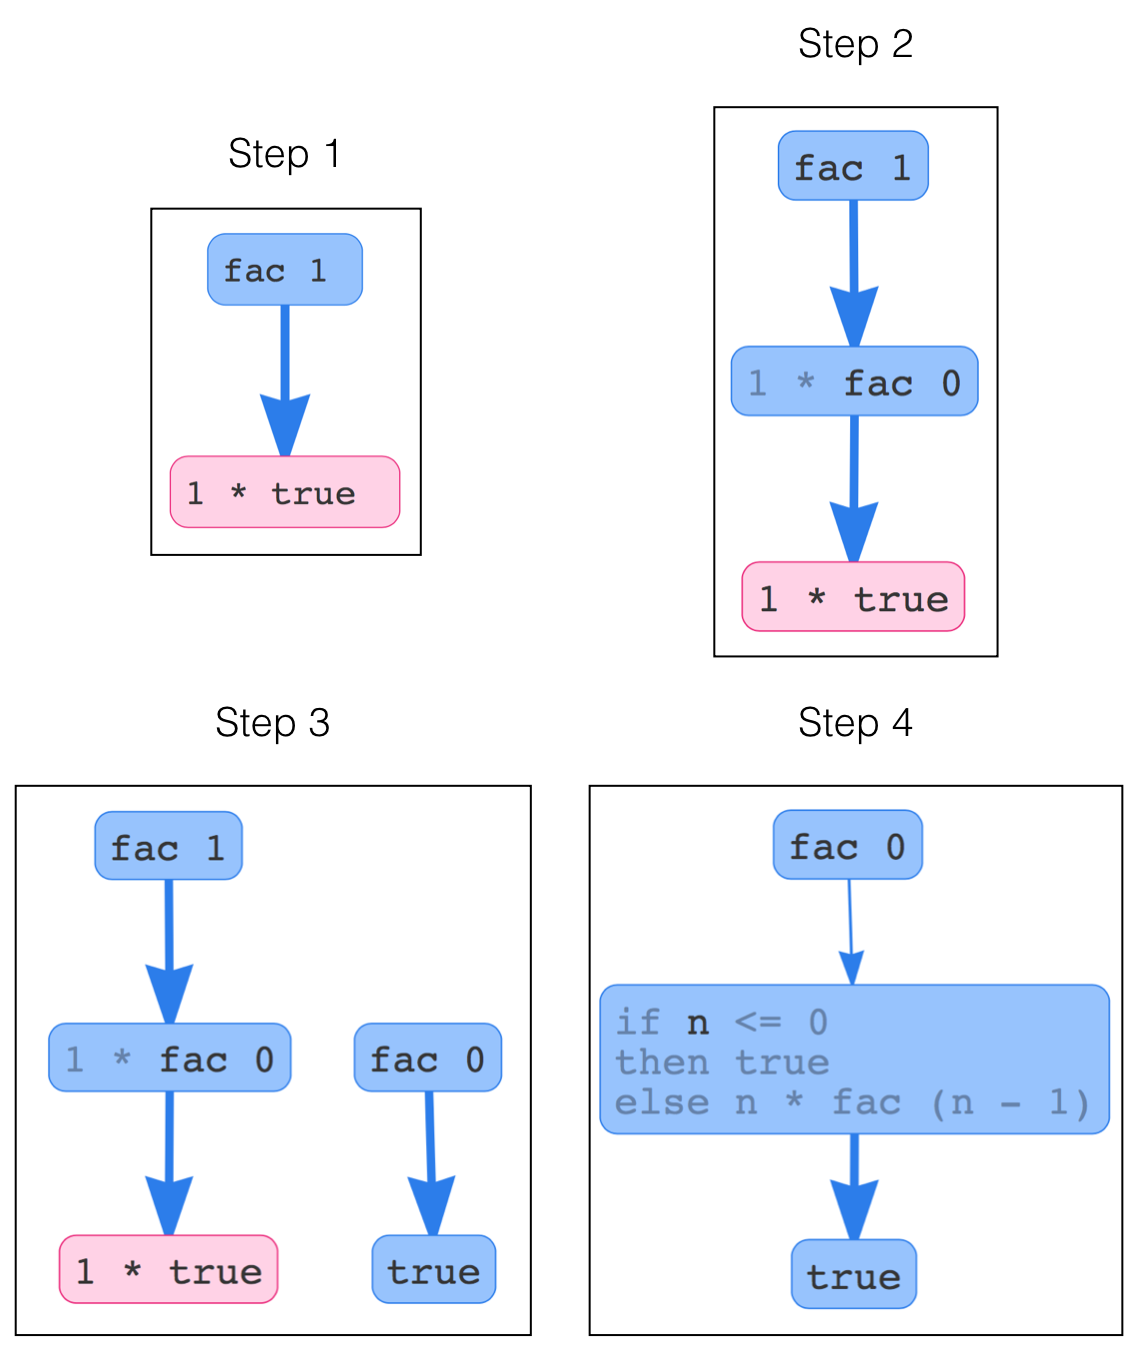
\includegraphics[height=8cm]{nanomaly/fac-steps-new.png}
\caption{A sequence of interactions with the trace of
  \texttt{fac 1}. The stuck term is red, in each node the redex is
  highlighted. Thick arrows denote a multi-step transition, thin arrows
  denote a single-step transition. We start in step 1. In step 2 we jump
  forward from the witness to the next function call. In step 3 we step
  into the recursive \texttt{fac 0} call, which spawns a new ``thread''
  of execution. In step 4 we take a single step forward from
  \texttt{fac 0}.}
\label{fig:nanomaly-factorial}
\end{figure}


\paragraph{Visualization State}
%
A \emph{visualization state} $\vstate$ is a \emph{directed graph}
whose vertices are expressions and whose edges are such
that each vertex has at most one predecessor and at most one
successor. In other words, the visualization state looks
like a set of linear lists of expressions as shown in
Figure~\ref{fig:nanomaly-factorial}.
%
The \emph{initial state} is the graph containing a single
edge linking the initial and final expressions.
\paragraph{Visualization Context}
%
The \emph{visualization context} of each expression $e$
in the visualization state $\vstate$ is the (unique) linear chain
in which the expression $e$ belongs.
%
We write $\vroot{\vstate}{e}$ for the \emph{first} (or root)
expression appearing in the visualization context of $e$ in
$\vstate$.

\paragraph{Commands}
Our debugger supports the following \emph{commands}, each of which
is parameterized by a single expression (vertex) selected from the
(current) visualization state:
%
\begin{itemize}
%
\item \stepforwardsym, \stepbackwardsym:
      show the result of a single step forward or backward respectively,
%
\item \jumpforwardsym, \jumpbackwardsym:
      show the result of taking multiple steps (a \emph{``big''} step)
      upto the first beta-reduction forward or backward respectively,
%
\item \stepintosym:
      show the result of stepping into a function call in a sub-term,
      isolating it from the context,

\item \stepoversym:
      show the result of skipping over a function call in a sub-term.
\end{itemize}

\begin{figure*}[t]
\[
\boxed{
\begin{array}{lcl}
\stepforward{\vstate}{e}  & \defeq
  & e' \quad \mbox{where } \singlestep{e}{e'} \in \tr \\ \\

\stepbackward{\vstate}{e} & \defeq
  & e' \quad \mbox{where } \singlestep{e'}{e} \in \tr \mbox{ and } e' \in \vpath{\vstate}{e} \\ \\

\jumpforward{\vstate}{e} & \defeq
  & \begin{cases}
    e'                         & \mbox{if } e' = \eapp{v}{v'} \\
    \jumpforward{\vstate}{e'}  & \text{otherwise}
    \end{cases}
    \mbox{\quad where } e' = \stepforward{\vstate}{e} \\ \\

\jumpbackward{\vstate}{e} & \defeq
  & \begin{cases}
    e'                         & \mbox{if } e' = \eapp{v}{v'} \\
    \jumpbackward{\vstate}{e'} & \text{otherwise}
    \end{cases}
    \mbox{\quad where } e' = \stepbackward{\vstate}{e} \\ \\

\stepinto{\vstate}{e} & \defeq
  & e'\sub{x}{v'} \quad \mbox{if } e = C[\eapp{v}{v'}] \mbox{ and } \singlestep{\eapp{v}{v'}}{e'\sub{x}{v'}}  \\ \\

\stepover{\vstate}{e} & \defeq
  & C[v''] \quad \mbox{if } e = C[\eapp{v}{v'}] \mbox{ and } \multistep{\eapp{v}{v'}}{v''} \in \tr \\[0.25in]

\vpath{\vstate}{e} & \defeq
  & \{e' \spmid \multistep{\vroot{\vstate}{e}}{e'} \in \tr
                \mbox{ and }
                \multistep{e'}{e} \in \tr \} \\[0.15in]
\end{array}
}
\]
\caption{Rules for computing the \emph{next} term given a
         visualization state $\vstate$, selected term $e$
         and command.}
\label{fig:traversing-graph}
\end{figure*}


\paragraph{Update}
%
Figure~\ref{fig:traversing-graph} shows
how we compute the \emph{next} expression
(to be added to the visualization state)
given the current visualization state
$\vstate$, command $\cmd$ and selected
expression $e$.
%
It is straightforward to then \emph{update}
the visualization graph by adding the new
term before (resp.\ after) the selected
expression $e$ if the command was a step
or jump forward (resp.\ backward), or
to create a new visualization context
if the command was $\stepintosym$.

%%% and \updState{\vstate}{\cmd}{e} then updates the graph
%%% by inserting the new expression appropriately, using
%%% one of the following graph manipulating functions:
%%% %
%%% \putBefore{\vstate}{e}{e'} (resp. \putAfter{\vstate}{e}{e'})
%%% returns the modified version of \vstate\ where $e'$ is the
%%% immediate predecessor of $e$ (resp.\ the immediate successor of $e$);
%%% %
%%% \putRoot{\vstate}{e}{e'} returns the modified version of \vstate
%%% extended with a new root vertex $e$ with successor $e'$.
%%% %
%%% @getNext vs e@ returns the immediate successor of @e@ in $\tr$.
%%% %
%%% @getPrev vs e@ computes the path @p@ between @e@ and its immediate
%%% predecessor in the current visualization, and then returns @e@'s immediate
%%% predecessor along @p@.
%%% %
%%% @getSubterms vs e@ traverses the sub-term edges to decompose an
%%% expression into a list of sub-expressions paired with their context.
%%% %
%%% @applyCtx vs e ctx@ applies @ctx@ to @e@, traversing the sub-term edges
%%% in reverse to find the super-term of @e@.
%%% %
%%% \hbox{@findApp vs e@} builds on top of @getSubterms@ to find the first
%%% application sub-term (if any), \ie the first sub-term that looks like
%%% $\eapp{v_1}{v_2}$.
%%% %
%%% @findVal vs e@ traverses the single-step edges to find the final value
%%% that @e@ reduces to.

% \section{Evaluation: Recasting Type Errors as Runtime Errors}
\section{Evaluation}
\label{sec:nanomaly:evaluation}

We have implemented a prototype of our search procedure and trace
visualization for a purely functional subset of \ocaml\ --- with
polymorphic types and records, but no modules, objects, or polymorphic
variants --- in a tool called \nanomaly.
%
We treat explicit type signatures, \eg @(x : int)@, as
primitive operations that narrow the type of the wrapped value.
%
In our implementation we instantiated \gensym\ with a simple random
generation of values, which we will show suffices for the majority of
type errors.

\paragraph{Evaluation Goals}
%
There are four questions we seek to answer with our evaluation:
%
\begin{enumerate}
\item \emphbf{Witness Coverage} (\S~\ref{sec:nanomaly:eval:witness-coverage},~\ref{sec:nanomaly:how-safe})
      How many ill-typed programs \emph{admit} witnesses?
\item \emphbf{Witness Complexity} (\S~\ref{sec:nanomaly:trace-complexity})
      How \emph{complex} are the traces produced by the witnesses?
\item \emphbf{Witness Utility} (\S~\ref{sec:nanomaly:advantage-traces},~\ref{sec:nanomaly:user-study})
      How \emph{helpful} %(qualitatively and quantitatively)
      are the witnesses in debugging type errors?
\item \emphbf{Witness-based Blame} (\S~\ref{sec:nanomaly:locating})
      Can witnesses be used to \emph{locate} the source
      of an error?
\end{enumerate}

In the sequel we present our experimental methodology (\S~\ref{sec:nanomaly:methodology})
and then answer the above questions.
%
However, for the impatient reader, we first summarize our main results:

\paragraph{1. Most Type Errors Admit Witnesses}
Our prime result is that the vast majority of static type errors, around
85\%, do in fact admit a dynamic witness.
%
Further, \toolname efficiently synthesizes witnesses with its randomized search;
it can synthesize a witness for over 75\% of programs in under one second, \ie
fast enough for interactive use. %to be integrated into the edit-compile-debug cycle.
%

\paragraph{2. Jump-Compressed Traces Are Small}
We find that our jump-compression heuristic effectively abstracts the
pedestrian details of computation, compressing the median trace with
14--15 single-step reductions to only 4 jumps.
%
Over 80\% of programs have a jump-compressed trace with at most 10
jumps, providing a bird's-eye view from which we can launch a more
in-depth investigation.

\paragraph{3. Witnesses Help Novices}
A witness should also help programmers \emph{understand} and
\emph{fix} type errors.
%
We use a set of ill-typed student programs to show that \toolname's
witnesses effectively demonstrate the runtime error that the type
system prevented.
%
Furthermore, we find, in a study of undergraduate students, that
\toolname's witnesses lead to more accurate diagnoses and fixes of type
errors than \ocaml's type error messages.

\paragraph{4. Witnesses Assign Blame}
Finally, we present a simple heuristic that allows us to use witnesses
to \emph{automatically} assign blame for type errors.
%
We treat the values inside the stuck term as \emph{sources} of typing
constraints and the stuck term itself as a \emph{sink}, producing
a slice of the program that likely contains the error.
%
Using this heuristic, \toolname's witnesses are competitive with the
state-of-the-art localization tools \mycroft and \sherrloc.

\subsection{Methodology}
\label{sec:nanomaly:methodology}
We answer the first two questions on two sets of ill-typed programs,
\ie\ programs that were rejected by the \ocaml\ compiler because of a
type error.
%
The first dataset comes from the Spring 2014 undergraduate Programming
Languages (CSE 130) course at UC San Diego.
%
We recorded each interaction with the \ocaml\ top-level system over the
course of the first three assignments (IRB
% \# hidden for blind review),
\#140608),
from which we extracted \ucsdsize\ distinct, ill-typed \ocaml\ programs
from a cohort of 46 students.
%
The second dataset --- widely used in the literature --- comes from a
graduate-level course at the University of Washington~\cite{Lerner2006-pj},
from which we extracted 284 ill-typed programs.
%
Both datasets contain relatively small programs, the largest being 348
SLoC; however, they demonstrate a variety of functional programming
idioms including (tail) recursive functions, higher-order functions,
and polymorphic and algebraic data types. % and expression evaluators.

We answer the third question in two steps.
%
First, we present a qualitative evaluation of \toolname's traces on a
selection of programs drawn from the UCSD dataset.
%
Second, we present a quantitative user study of students in the
University of Virginia's Spring 2016 undergraduate Programming Languages
(CS 4501) course.
%
As part of an exam, we presented the students with ill-typed \ocaml\
programs and asked them to
%
(1) \emph{explain} the type error, and
%
(2) \emph{fix} the type error (IRB \#2014009900).
%
For each problem the students were given the ill-typed program and
either \ocaml's error message or \toolname's jump-compressed trace.

We answer the last question on a subset of the \ucsdbench dataset.
%
% For each ill-typed program in a student's interaction trace, we identify
% the student's \emph{fix} by searching for the first type-correct program
% that follows it in the trace.
For each ill-typed program compiled by a student, we identify the student's
\emph{fix} by searching for the first type-correct program that the student
subsequently compiled.
%
We then use an expression-level \emph{diff}~\cite{Lempsink2009-xf} to
determine which sub-expressions changed between the ill-typed program
and the student's fix, and treat those expressions as the source of the
type error.

\subsection{Witness Coverage}
\label{sec:nanomaly:eval:witness-coverage}
%
We ran our search algorithm on each program for 1,000 iterations, with
the entry point set to the function that \ocaml\ had identified as
containing a type error.
%
Due to the possibility of non-termination we set a timeout of one minute
total per program.
%
% Due to the possibility of non-termination we set a limit on the number
% of reductions to perform, increasing in 500-step increments from 500
% steps to 3,000 steps total.
%
We also added a na{\"\i}ve check for infinite recursion; at each recursive
function call we check whether the new arguments are identical to the
current arguments.
%
If so, the function cannot possibly terminate and we report an error.
%
While not a \emph{type error}, infinite recursion is still a clear bug
in the program, and thus valuable feedback for the user.

\begin{figure}[t]
% \centerline{
% \begin{minipage}{1.2\textwidth}
\centering
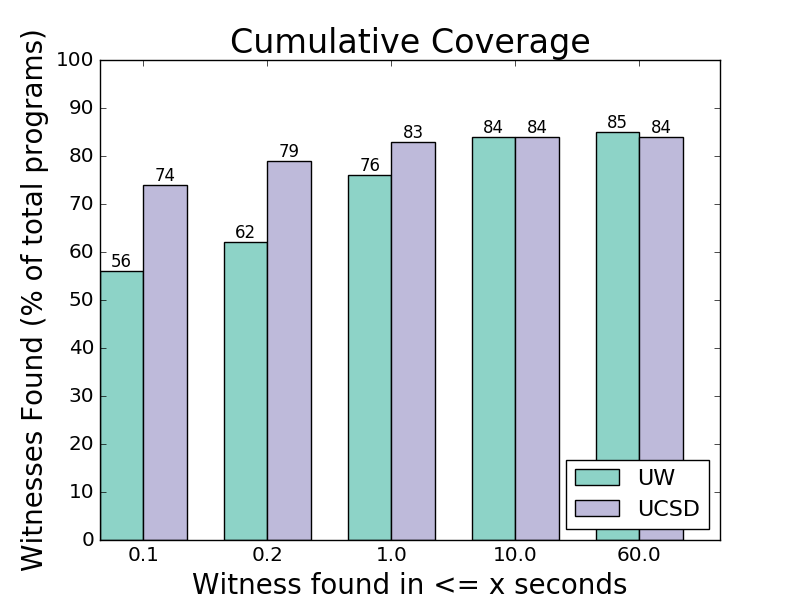
\includegraphics[width=0.8\linewidth]{nanomaly/coverage.png}
% \end{minipage}
% \begin{minipage}{\linewidth}
% \includegraphics[width=0.6\linewidth]{distrib.png}
% \end{minipage}
% }
% \vspace{3ex}
\caption{Results of our coverage testing. Our random search successfully
  finds witnesses for 76--83\% of the programs in under one second,
  improving to 84--85\% in under 10 seconds. }
\label{fig:results-witness}
\end{figure}
\begin{figure}[t]
\centering
\includegraphics[width=0.8\linewidth]{nanomaly/distrib.png}
\caption{Distribution of test outcomes. In both datasets we detect
  actual type errors at least 77\% of the time, unbound variables or
  constructors 4\% of the time, and diverging loops 2--3\% of the
  time. For the remaining 15--16\% of the programs we are unable to
  provide any useful feedback. }
\label{fig:results-distrib}
\end{figure}


\paragraph{Results}
\label{sec:nanomaly:results-witness}
The results of our experiments are summarized in
Figures~\ref{fig:results-witness}~and~\ref{fig:results-distrib}.
%
In both datasets our tool was able to find a witness for over 75\% of the
programs in under one second, \ie\ fast enough to be integrated as a
compile-time check. If we extend our tolerance to a 10 second timeout,
we reach 84\% coverage, and if we allow a 60 second search,
we hit a maximum of 84--85\% coverage.
%
Interestingly, while the vast majority of witnesses corresponded to a
type-error, as expected, 4\% triggered an unbound variable error (even
though \ocaml\ reported a type error) and 3\% triggered an infinite
recursion error.
%
For the remaining 15--16\% of programs we were unable to provide any useful
feedback as they either completed 1,000 tests successfully, or timed out
after one minute.
%
% XX programs were deemed safe and XX timed out even at 3,000 steps, \ie
% we could not provide any useful feedback for XX\% of the total programs.
%
While a more advanced search procedure, \eg\ dynamic-symbolic execution,
could likely uncover more errors, our experiments suggest that
type errors are coarse enough (or that novice programs are \emph{simple}
enough) that these techniques are not necessary.

\subsection{How safe are the ``safe'' programs?}
\label{sec:nanomaly:how-safe}

An immediate question arises regarding the 15--16\% of programs for
which we could not synthesize a witness:
%
are they \emph{actually} safe (\ie is the type system being too conservative),
%
or did \toolname simply fail to find a witness?
%
% \ES{Need better organization for the groupings of programs, maybe a pie chart to guide us?}

To answer this question, we investigated the 732 \ucsdbench programs for
which we failed to find a witness.
%
We used a combination of automatic and manual coding to categorize these
programs into four classes.
%
The first class is easily detected by \toolname itself, and thus admits
a precise count.
%
This left us with 504 programs that required manual coding; we selected
a random sample of 50 programs to investigate, and will report results
based on that sample.
%
Figure~\ref{fig:no-witness} summarizes the results of our investigation ---
we note the classes that were based on the random sample with a ``*''.


\begin{figure}[t]
\centering
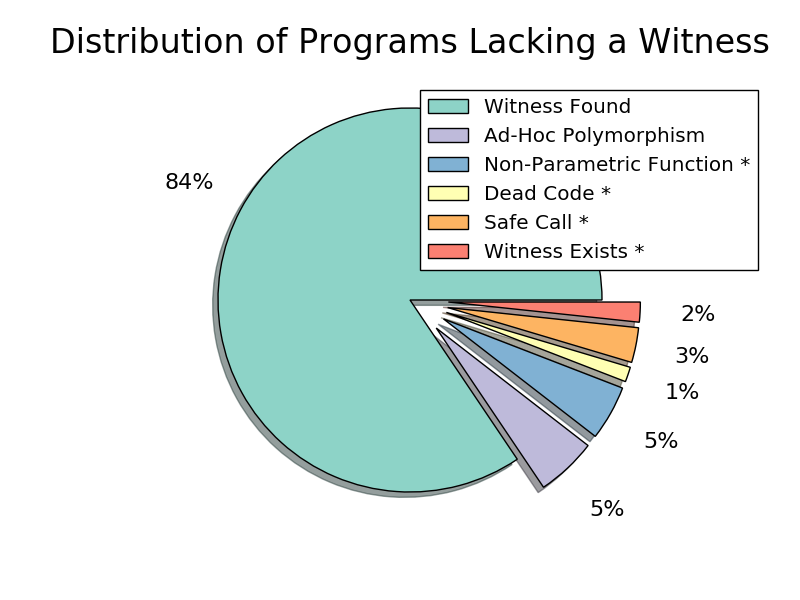
\includegraphics[width=0.7\linewidth]{nanomaly/distrib_ext.png}
\vspace{-0.75cm}
\caption{Results of our investigation into programs where \toolname
  did not produce a witness. A ``*'' denotes that the percentage is an
  estimate based on a random sampling of 50 programs.}
\label{fig:no-witness}
\end{figure}

\paragraph{Ad-Hoc Polymorphism}
%
We found that for 5\% programs \toolname got stuck when it tried to
compare two holes.
%
\ocaml provides polymorphic equality and comparison operators,
overloading them for each type.
%
While convenient to use, they pose a challenge for \toolname's
combination of execution and inference.
%
For example, % consider the \hbox{@n <= 0@} test in our @fac@ example.
% %
% The @<=@ operator is polymorphic, but in this case we can make progress because
% the literal @0@ is not.
% %
% Suppose, however, we parameterized @fac@ by a lower bound, \eg
% %
consider the following ill-typed factorial function, parameterized by a
lower bound.
%
\begin{code}
  let rec fac n m =
    if n <= m then
      true
    else
      n * fac (n - 1) m
\end{code}
%
When given @fac@, \toolname will generate two fresh holes
$\nu_1^{\alpha_1}$ and $\nu_2^{\alpha_2}$ and proceed directly into the
@n <= m@ comparison.
%
We cannot (yet) instantiate either hole because we have no constraints
on the $\alpha$s (we know they must be equal, but nothing else), and
furthermore we do not know what constraints we may encounter later on in
the program.
%
Thus, we cannot perform the comparison and proceed, and must give up our
search for a witness, even though one obviously exists, any pair of |n|
and |m| such that |n <= m| is false.

Extending \toolname with support for symbolic execution would alleviate
this issue, as we could then begin symbolically executing the program
until we learn how to instantiate |n| and |m|.
%
Alternatively, we could \emph{speculatively} instantiate both |n| and
|m| with some arbitrary type, and proceed with execution until we
discover a type error.
%
This speculative instantiation is, of course, unsound; we would have to
take care to avoid reporting frivolous type errors that were caused by
such instantiations.
%
We would need to track which holes were instantiated speculatively 
to distinguish type errors that would have happened regardless, as
in @fac@, from type errors that were caused by our instantiation.

Further, suppose that our speculative instantiation induces a frivolous
type error.
%
For example, suppose we are given
%
\begin{code}
  let bad x y =
    if x < y then
      x *. y
    else
      0.0
\end{code}
%
and choose to (speculatively) instantiate @x@ and @y@ as @int@s and proceed
down the ``true'' branch.
%
We will quickly discover this was the wrong choice, as they are immediately
narrowed to @float@s.
%
We must now backtrack and try a different instantiation, but we no
longer need to choose one at random.
%
Since our instantiation was speculative, and @x@ and @y@
% WRW thinks "morally" is too informal for this venue. 
were \emph{originally} holes, we can treat the @*.@ operator as a normal
narrowing point with two holes.
%
This tells us that the \emph{correct} instantiation was in fact @float@,
and we can then proceed as normal from the backtracking point with a
concrete choice of @float@s.
%
Thus, it appears that speculative instantiation of holes may be a
useful, lightweight alternative to symbolic execution for our purposes.

% \paragraph{} \hspace{0ex} \\
% The remaining 473 programs for which we could not produce a witness did
% not admit such an automatic diagnosis, so we selected a random sample of
% 50 programs and manually searched for a witness.
% %
% We categorized the programs into three groups.


\paragraph{Non-Parametric Function Type *}
%
5\% of programs lack a witness in our semantics due to our
non-parametric $\tfun$ type for functions.
%
Recall that our goal is to expose the runtime errors that would have
been prevented by the type systems.
%
At runtime, it is always safe to call a function, thus we give functions
a simple type $\tfun$ that says they may be applied, but says nothing
about their inputs or outputs.
%
But consider the following @clone@ function, which is supposed to
produce a list containing @n@ copies of the input @x@.
%
% Seven programs violated the \emph{occurs check} with cyclic typing
% constraints like @'a = 'a list@, for example the following @clone@
% function.
%
\begin{code}
  let rec clone x n =
    if n > 0 then
      clone [x] (n - 1)
    else
      []
\end{code}
%
Unfortunately, the student instead constructs an @n@-level nested list
containing a single @x@.
%
The \ocaml compiler rejects this program because the recursive call to
@clone@ induces a cyclic typing constraint @'a = 'a list@, capturing the
fact that each call increases the nesting of the list.
%
\toolname fails to catch this because we do not track the types of the
inputs to @clone@.

We note, however, that @clone@ cannot go wrong; it is perfectly safe to
repeatedly enclose a list inside another (disregarding the fact that the
nested list is never returned).
%
Still, such a function would be very difficult to \emph{call} safely, as
the programmer would have to reason about the dependency between the
input @n@ and the nesting of the output list, which cannot be expressed
in \ocaml's type system.

Thus, it is not particularly satisfying that \toolname fails to produce
a witness here; a possible solution could be to track the types of the
inputs, and demonstrate to the user how they change between recursive
calls.
%
This would require maintaining a typing environment of variables in
addition to the environments we maintain for holes.
%
We would have to modify the rule $\reappgood$ from
Figure~\ref{fig:operational} to additionally $\forcesym$ the function's
type against the concrete inputs.
%
However, we would want to ensure that this $\forcesym$ cannot fail ---
it is preferable to report a stuck term as that provides a fuller view
of the error.
%
Rather, we would note which evaluation steps induced incompatible
type refinements, and if a traditional witness cannot be found, we could
then report a trace expanded to show precisely these steps.
%
This represents only a modest extension to our semantics, and would be
interesting to explore further.

\paragraph{Dead Code and ``Safe'' Function Calls *}
%
4\% of programs contained type errors that were unreachable, either
because they were dead code, or because the student called the function
with inputs that could not trigger the error.


1\% contained type errors that were unreachable by any inputs, often due
to overlapping patterns in a @match@ expression.
%
% While technically safe, dead code is generally considered a ``code
% smell''; students would likely benefit from a warning in this case.
% \ES{Wes says this is too informal, source the claim}
%
While technically safe, dead code is generally considered a maintenance
risk, as the programmer may not realize that it is dead~\cite{Wheeler2014-fg}
or may accidentally bring it back to life~\cite{Seven2014-gf}.
%
Thus, a warning like that provided by \ocaml's pattern exhaustiveness
checker would be helpful.

%\paragraph{Bad Function Calls}
A further 3\% included a function call where the
student supplied ill-typed inputs, but the path induced
by the call did not contain an error.
%
Consider the following |assoc| function, which
looks up a key in an \emph{association list}, returning a default if
it cannot be found.
%
\begin{code}
  let rec assoc (d, k, l) = match l with
    | (ki, vi)::tl ->
       if ki = k then
         vi
       else
         assoc (d, k, tl)
    | _ -> d

  let _ = assoc ([], 123, [(123, "sad"); (321, "happy")])
\end{code}
%
The student's definition of |assoc| is correct, but \ocaml rejects their
subsequent call because the default value |[]| is incompatible with the
|string| values in the list.
%
In this particular call the key |123| is in the list, so the default
will not be used (even if it were, there would not be an error) and
\ocaml's complaint is moot.
%
Of course, \ocaml cannot be expected to know that this particular call
is safe, its type system is not sophisticated enough to express the
necessary conditions.
%
% \ES{TODO: add some comment about using dependent types, though this particular example would be quite bizarre to encode in DT..}

% We note that many of the programs in this category appear to come from
% interactions with the \ocaml top-level, \ie the student defined a
% function and is now experimenting with it.
% %
% These calls are thus particularly harmless, indeed they may even be
% \emph{beneficial}, as the student may next try looking up a key that
% \emph{does not} exist, and realize that the returned values are
% incompatible.
% \ES{Wes doesn't like this, sounds like punting on the issue}

\paragraph{Witness Exists *}
%
We found that only 2\% of programs admit a witness that \toolname
was unable to discover.
%
Slightly over half involved synthesizing a \emph{pair} of
specially-crafted inputs that would result in the function returning
values of incompatible types.
%
The rest required synthesizing an input that would trigger a
particular path through the program, and would likely have been caught
by symbolic execution.

\paragraph{Summary}
%
Our investigation suggests that the vast majority of programs
for which we fail to find a witness do not, in fact, admit a
witness.
%
% Overall, it appears that our random instantiation of holes is well-suited
% to finding type errors in student programs.
These programs were generally cases where \ocaml's type system was
overly conservative.
%
Of course, the conservatism is somewhat justified as each case pointed
to code that would be difficult to use or maintain;
%
it would be interesting to investigate how demonstrate these issues in an
intuitive manner.

% \begin{enumerate}
% \item 7 infinite type. program doesn't go wrong, but could search for
%   context that would go wrong
% \item 15 monomorphic functions. recall we abstract a function's type as
%   $\tfun$ rather than $\alpha \to \beta$. (may also admit witness by
%   searching for context?)
% \item 6 dead code. type error occurs in unreachable code, ``deficiency''
%   of the type system.
% \item 14 bad call. function is well-typed, student calls makes ill-typed
%   call, but no error triggered. nothing to be done, as we do not control
%   call-site.
% \end{enumerate}

%%% Local Variables:
%%% mode: latex
%%% TeX-master: "main"
%%% End:



\subsection{Witness Complexity}
\label{sec:nanomaly:trace-complexity}

For each of the ill-typed programs for which we could
find a witness, we measure the complexity of the generated
trace using two metrics.

% \paragraph{Metrics} Thus, our two metrics are:
% size of the full trace,
% \ie the number of small-step reductions, and the size of the jump-compressed
% version of the trace.
%
\begin{enumerate}
\item \emphbf{Single-step:} The size of the trace after expanding
  all of the single-step edges from the witness to the stuck term, and
  % This can be thought of as a worst-case
  % complexity, \ie ``How big is the fully-expanded trace?''
\item \emphbf{Jump-compressed:} The size of the jump-compressed trace.
\end{enumerate}


% \item \ES{others?}
%
\begin{figure}[t]
% \centerline{
% \begin{minipage}{1.2\textwidth}
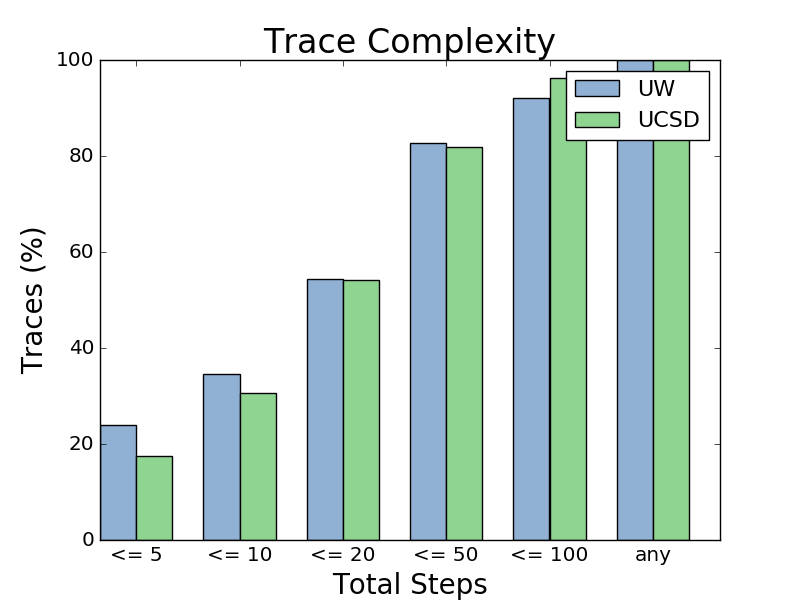
\includegraphics[width=0.7\linewidth]{nanomaly/trace_size_step.png}
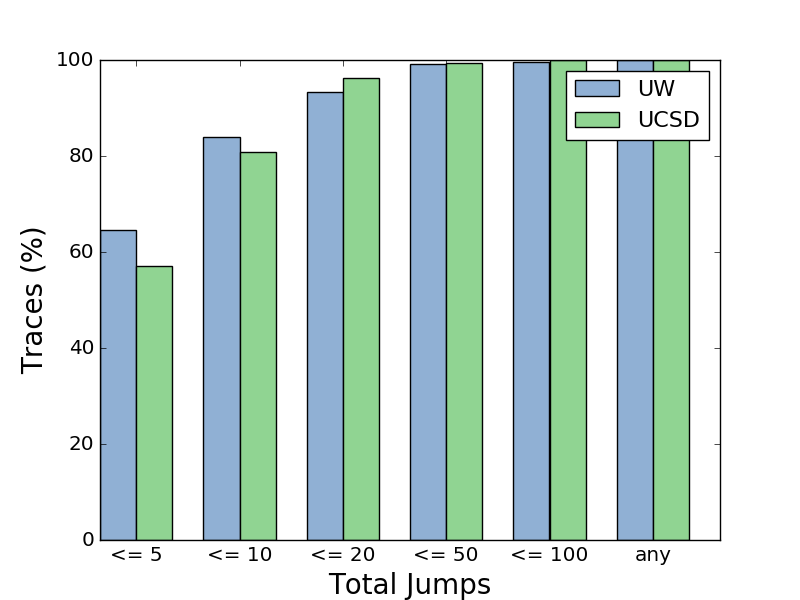
\includegraphics[width=0.7\linewidth]{nanomaly/trace_size_jump.png}
% \end{minipage}
% }
% \vspace{3ex}
\caption{Complexity of the generated traces. Over 80\% of the combined traces
  have a jump complexity of at most 10, with an average complexity of 7
  and a median of 5.}
\label{fig:results-complexity}
\end{figure}
%
\paragraph{Results}
\label{sec:nanomaly:results-complexity}
The results of the experiment are summarized in
Figure~\ref{fig:results-complexity}.
%
The average number of single-step reductions per trace is 17 for the
\ucsdbench\ dataset (42 for the \uwbench\ dataset) with a maximum of
2,745 (\resp 982) and a median of 15 (\resp 15).
%
The average number of jumps per trace is 7 (\resp 9) with a
maximium of 353 (\resp 221) and a median of 4 (\resp 4).
%
In both datasets about 60\% of traces have at most 5 jumps, and 80\% or more
have at most 10 jumps.


\subsection{Qualitative Evaluation of Witness Utility}\label{sec:nanomaly:advantage-traces}

Next, we present a \emph{qualitative} evaluation that compares
the explanations provided by \toolname's dynamic witnesses with
the static reports produced by the \ocaml\ compiler and \sherrloc,
a state-of-the-art fault localization approach~\cite{Zhang2014-lv}.
%
In particular, we illustrate, using a series of examples drawn
from student programs in the \ucsdbench\ dataset, how \toolname's
jump-compressed traces can get to the heart of the error. Our approach
%
highlights the conflicting values that cause the program to get
stuck, rather that blaming a single one,
%
shows the steps necessary to reach the stuck state, and
%
does not assume that a function is correct just because it type-checks.
%
For each example we will present:
(1)~the code;
(2)~the error message returned \ocaml;
(3)~the error locations returned by \hlOcaml{\ocaml} and \hlSherrloc{\sherrloc};
and (4)~\toolname's jump-compressed trace.

% \begin{figure*}[ht]
% \centering
% \begin{minipage}{0.49\linewidth}
% \centering

% \begin{figure*}[htp]
%   \centering
%   \includegraphics[height=125px]{sqsum.png}
%   \includegraphics[height=125px]{sumlist.png}
%   \includegraphics[height=150px]{digitsOfInt.png}
%   \includegraphics[height=125px]{wwhile.png}
%   \caption{(Left to right) Jump-compressed traces showing how
%     \texttt{sqsum}, \texttt{sumList}, \texttt{digitsOfInt}, and
%     \texttt{wwhile} go wrong in \S~\ref{sec:nanomaly:advantage-traces}.}
%   \label{fig:traces}
% \end{figure*}

\paragraph{Example: Recursion with Bad Operator}
The recursive function @sqsum@ should square each
element of the input list and then compute the sum
of the result.
%
\begin{ecode}
  let rec sqsum xs = match xs with
    | [] -> 0
    | h::t -> (*@\hlOcaml{\hlSherrloc{sqsum t}}@*) @ (h * h)
\end{ecode}
%
Unfortunately the student has used the list-append
operator |@| instead of \texttt{+}. % to compute the sum.
%
Both \ocaml\ and \sherrloc\ blame the \emph{wrong location},
the recursive call @sqsum t@, with the message
%
\begin{verbatim}
  This expression has type
    int
  but an expression was expected of type
    'a list
\end{verbatim}
%
\toolname\ produces a trace showing how the evaluation of
@sqsum [1]@ gets stuck.
%
\begin{center}
  \includegraphics[height=125px]{nanomaly/sqsum.png}
\end{center}
%
The trace highlights the entire stuck term
(not just the recursive call), emphasizing
the \emph{conflict} between @int@ and @list@
rather than assuming one or the other is correct.

\paragraph{Example: Recursion with Bad Base Case}
%
The function @sumList@ should add up
the elements of its input list.
%
\begin{ecode}
  let rec sumList xs = match xs with
    | []    -> (*@\hlSherrloc{[]}@*)
    | y::ys -> y + (*@\hlOcaml{sumList ys}@*)
\end{ecode}
%
Unfortunately, in the base case, it returns @[]@
instead of @0@.
%
\sherrloc\ blames the base case, and \ocaml\
assumes the base case is correct and blames
the \emph{recursive call} on line 3:
%
\begin{verbatim}
  This expression has type
    'a list
  but an expression was expected of type
    int
\end{verbatim}
%
Both of the above are parts of the full story, which
is summarized by \toolname's trace showing
how @sumList [1; 2]@ gets stuck at @2 + []@.
%
\begin{center}
  \includegraphics[height=125px]{nanomaly/sumlist.png}
\end{center}
%
The trace clarifies (via the third step)
that the @[]@ results from the recursive call
\hbox{@sumList []@,} and shows how it is incompatible with
the subsequent \texttt{+} operation.

%% ES: append is actually a bit problematic as we don't find the nice
%% append [1] [2] witness. instead we could find something like
%% append [_] [], but it's not as clear IMO
% Our next example is the @append@ function, which should concatenate the
% two input lists.
% %
% \begin{ecode}
% let append xs ys = match xs with
%   | []   -> ys
%   | h::t -> h :: __t__ :: ys
% \end{ecode}
% %
% The student has forgotten to make a recursive call to @append@, and
% instead tries to cons the tail @t@ directly onto the second list @ys@.
% Consing @h@ back onto the result causes \ocaml to attempt to construct
% the infinite type @'a = 'a list@, triggering an \emph{occurs-check}
% error.
% %
% \begin{verbatim}
% Error: This expression has type
%          'a list
%        but an expression was expected of type
%          'a
%        The type variable 'a occurs inside 'a list
% \end{verbatim}
% %
% %
% \begin{center}
%   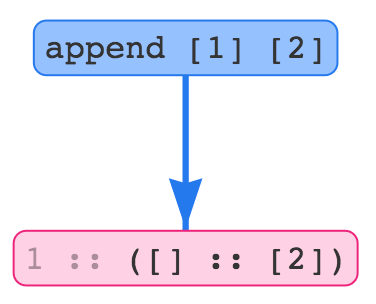
\includegraphics[height=75px]{append.png}
% \end{center}

%\pagebreak
\paragraph{Example: Bad Helper Function that Type-Checks}
%
The function @digitsOfInt@ should return a list of
the digits of the input integer.
%
\begin{ecode}
  let append x xs =
    match xs with
    | [] -> [x]
    | _  -> x :: xs

  let rec digitsOfInt n =
    if n <= 0 then
      []
    else
      append ((*@\hlSherrloc{digitsOfInt (n / 10)}@*)) [(*@\hlOcaml{n mod 10}@*)]
\end{ecode}
%
%\pagebreak
Unfortunately, the student's @append@ function \emph{conses} an element
onto a list instead of appending two lists.
%
Though incorrect, @append@ still type-checks and thus \ocaml and
\sherrloc blame the \emph{use-site} on line 10.
%
\begin{verbatim}
  This expression has type
    int
  but an expression was expected of type
    'a list
\end{verbatim}
%
In contrast, \toolname makes no assumptions about @append@,
yielding a trace that illustrates the error on line 4, by
highlighting the conflict in consing a list onto a list of integers.
%
\begin{center}
  \includegraphics[height=160px]{nanomaly/digitsOfInt.png}
\end{center}
%

\paragraph{Example: Higher-Order Functions}
%
The higher-order function @wwhile@ is supposed
to emulate a traditional while-loop. It takes
a function @f@ and repeatedly calls @f@ on the
first element of its output pair, starting with
the initial @b@, till the second element is @false@.
%
\begin{ecode}
  let rec wwhile (f,b) =
    match f with
    | (z, false) -> z
    | (z, true)  -> wwhile (f, z)

  let f x =
    let xx = x * x in
    (xx, (xx < 100))

  let _ = wwhile ((*@\hlOcaml{\hlSherrloc{f}}@*), 2)
\end{ecode}
%
The student has forgotten to \emph{apply} @f@ at all on line 2,
and just matches it directly against a pair.
This faulty @wwhile@ definition nevertheless typechecks,
and is assumed to be correct by both \ocaml\ and \sherrloc\
which blame the use-site on line 10.
%
\begin{verbatim}
  This expression has type
    int -> int * bool
  but an expression was expected of type
    'a * bool
\end{verbatim}
%
\toolname\ synthesizes a trace that draws the eye to the
true error: the @match@ expression on line 2, and highlights
the conflict in matching a function against a pair pattern.
%
\begin{center}
  \includegraphics[height=135px]{nanomaly/wwhile.png}
\end{center}
%
By highlighting conflicting values, \ie\ the source and sink
of the problem, and not making assumption about function correctness, \toolname\
focusses the user's attention on the piece of code that is
actually relevant to the error.

\subsection{Quantitative Evaluation of Witness Utility}
\label{sec:nanomaly:user-study}
% Finally, to test the explanatory power of our jump-compressed traces, we
% ran a user study (IRB \#2014009900) at the University of Virginia (UVA).
% %
% We included four problems in an exam in the Spring session of UVA's
% undergraduate Programming Languages course (CS 4501).
% %
% We presented the 60 students in the course with ill-typed \ocaml\
% programs and asked them to
% %
% (1) \emph{explain} the type error, and
% %
% (2) \emph{fix} the type error.
% %
% For each problem the student was given the ill-typed program and
% either \ocaml's error message or \toolname's jump-compressed trace.
%
We assigned four problems to the 60 students in the course: the
@sumList@, \hbox{@digitsOfInt@,} and @wwhile@ programs from
\S~\ref{sec:nanomaly:advantage-traces}, as well as the following @append@ program
%
\begin{ecode}
  let append x l =
    match x with
    | []   -> l
    | h::t -> h :: t :: l
\end{ecode}
%
which triggers an occurs-check error on line 4.
%
For each problem the students were given the ill-typed program and
either \ocaml's error or \toolname's jump-compressed trace;
the full user study is available in \autoref{sec:nanomaly:user-study-exams}.
%
Due to the nature of an in-class exam, not every student answered every
question; we received between 13 and 28 (out of a possible 30) responses
for each problem-tool pair.

We then instructed four annotators (one of whom is an author, the other
three are teaching assistants at UCSD) to classify the answers as
correct or incorrect.
%
We performed an inter-rater reliability (IRR) analysis to determine the
degree to which the annotators consistently graded the exams.
%
As we had more than two annotators assigning nominal (``correct'' or
``incorrect'') ratings we used Fleiss' kappa~\cite{Fleiss1971-du} to
measure IRR.\@
%
Fleiss' kappa is measured on a scale from $1$, indicating total
agreement, to $-1$, indicating total disagreement, with $0$ indicating
random agreement.

Finally, we used a one-sided Mann-Whitney $U$ test~\cite{Mann1947-fd} to
determine the significance of our results.
%
The null hypothesis was that the responses from students given
\toolname's witnesses were drawn from the same distribution as those
given \ocaml's errors, \ie \toolname had no effect.
%
Since we used a one-sided test, the alternative to the null hypothesis
is that \toolname had a \emph{positive} effect on the responses.
%
We reject the null hypothesis in favor of the alternative if the test
produces a significance level $p < 0.05$, a standard threshold for
determining statistical significance.

\paragraph{Threats to Validity}
Measuring understanding is a difficult task; the following summarize
the threats to the validity of our results.

\subparagraph{Construct.}
%
We used the correctness of the student's explanation of, and fix for,
the type error as a proxy for her understanding, but it is possible
that other metrics would produce different results.

\subparagraph{Internal.}
%
We assigned students randomly to two groups. The first was given
\ocaml's errors for @append@ and @digitsOfInt@, and \toolname's trace
for @sumList@ and @wwhile@; the second was given the opposite
assignment of errors and traces. This assignment ensured that: (1) each
student was given \ocaml and \toolname problems; and (2) each student
was given an ``easy'' and ``hard'' problem for both \ocaml and
\toolname. Students without sufficient knowledge of \ocaml could affect
the results, as could the time-constrained nature of an exam. For these
reasons we excluded any answers left blank from our analysis.

\subparagraph{External.}
%
Our experiment used students in the process of learning \ocaml,
and thus may not generalize to all developers. The four
programs were chosen manually, via a random selection and
filtering of the programs in the \ucsdbench dataset. In some cases we made
minor simplifying edits (\eg alpha-renaming, dead-code removal) to the
programs to make them more understandable in the short timeframe of an
exam; however, we never altered the resulting type-error. A different
selection of programs may lead to different results.

\subparagraph{Conclusion.}
%
We collected exams from 60 students, though due to the nature of the
study not every student completed every problem.
%
The number of complete submissions ranges from 13 (for the \toolname
version of @wwhile@) to 28 (for the \ocaml version of @sumList@), out of
a maximum of 30 per program-tool pair.
%
Our results are statistically significant in only 2 out of 8 tests; however,
collecting more responses per test pair was not possible as it
would require having students answer the same problem twice (once with
\ocaml and once with \toolname).

\begin{figure}[t]
% \centerline{
% \begin{minipage}{1.2\textwidth}
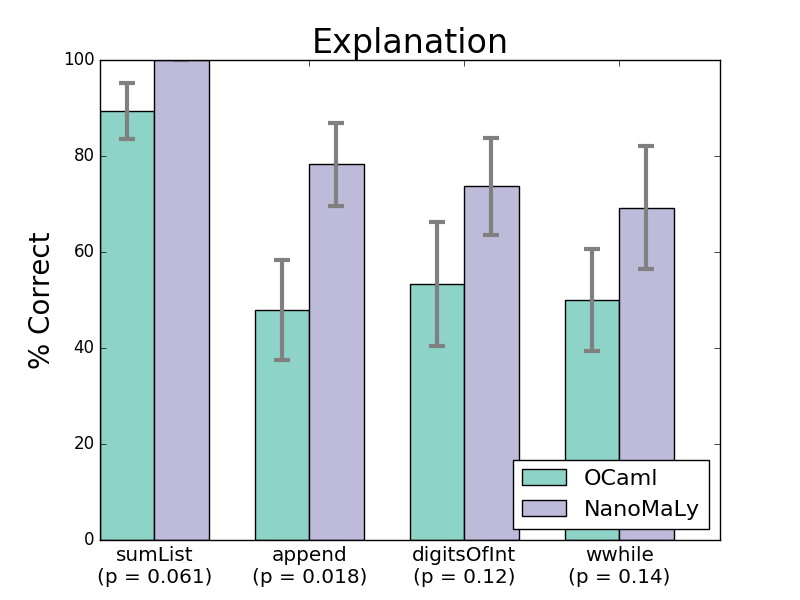
\includegraphics[width=0.7\linewidth]{nanomaly/user-study-reason.png}
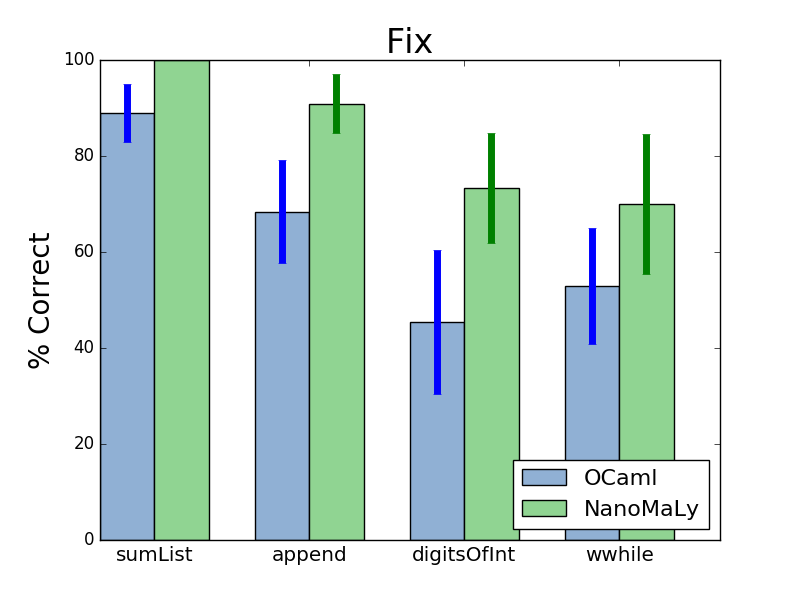
\includegraphics[width=0.7\linewidth]{nanomaly/user-study-fix.png}
% \end{minipage}
% }
% \vspace{3ex}
\caption{A classification of students' explanations and fixes for type
  errors, given either \ocaml's error message or \toolname's
  jump-compressed trace. The students given \toolname's jump-compressed
  trace consistently scored better ($\ge 10\%$) than those given
  \ocaml's type error. We report the result of a one-sided Mann-Whitney
  $U$ test for statistical significance in parentheses.}
\label{fig:results-user-study}
\end{figure}

\paragraph{Results}
%
The measured kappa values were $\kappa = 0.72$ for the explanations and
$\kappa = 0.83$ for the fixes; while there is no formal notion for what
consititutes strong agreement~\cite{Krippendorff2012-wd}, kappa values
above $0.60$ are often called ``substantial''
agreement~\cite{Landis1977-ey}.
%
Figure~\ref{fig:results-user-study} summarizes a single annotator's
results, which show that students given \toolname's jump-compressed
trace were consistently more likely to correctly explain
and fix the type error than those given \ocaml's error message.
%
Across each problem the \toolname responses were marked correct
$10-30\%$ more often than the \ocaml responses, which suggests that
the students who had access to \toolname's traces had a better
understanding of the type errors;
%
however, only the @append@ tests were statistically significant at
$p < 0.05$.
%


\subsection{Locating Errors with Witnesses}
\label{sec:locating}

We have seen that \toolname can effectively synthesize witnesses to
explain the majority of (novice) type errors, but a good error report
should also help \emph{locate} the source of the error.
%
Thus, our final experiment seeks to use \toolname's witnesses as
localizations.


As discussed in \S~\ref{sec:methodology}, we recorded
each interaction of our students with the \ocaml top-level system.
%
This means that, in addition to collecting ill-typed programs, we
collected subsequent, fixed versions of the same programs.
%
% For each ill-typed program in a student's interaction trace, we identify
% the student's fix by searching for the first type-correct program
% that follows it in the trace.
For each ill-typed program compiled by a student, we identify the student's
\emph{fix} by searching for the first type-correct program that the student
subsequently compiled.
%
We then use an expression-level \emph{diff}~\cite{Lempsink2009-xf} to
determine which sub-expressions changed between the ill-typed program
and the student's fix, and treat those expressions as the source of the
type error.

Not all ill-typed programs will have an associated fix; furthermore,
at some point a ``fix'' becomes a ``rewrite''.
%
We do not wish to consider the ``rewrites'', so we discard outliers
where the fraction of expressions that have changed is more than one
standard deviation above the mean, establishing a diff threshold of
45\%.
%
This accounts for roughly 14\% of programs pairs we discovered, leaving
us with 2,425 program pairs.

For each pair of an ill-typed program and its fix, we run \toolname and
collect two sets of source locations:
%
(1) the source location corresponding to the stuck term; and
%
(2) the source locations that \emph{produced} the values inside the
stuck term.
%
Intuitively, these two classes of locations correspond to \emph{sinks}
and \emph{sources} for typing constraints.
%
For example, in the @sqsum@ program from \S~\ref{sec:advantage-traces}
the stuck term is \verb!0 @ 1!.
%
This corresponds to the call to \verb!@! on line 3, and contains
the literal @0@ from line 2 and the value @1@ produced by the
@*@ on line 3.

We compare \toolname's witness-based predictions against a baseline of
the \ocaml compiler as well as the state-of-the-art %type error
localization tools \sherrloc and \mycroft.
%
\sherrloc~\cite{Zhang2014-lv} attempts to predict the most likely source
of a type error by searching the typing constraint graph for constraints
that participate in many unsatisfiable paths and few satisfiable paths.
%
\mycroft~\cite{Loncaric2016-uk} reduces the localization problem to
MaxSAT by searching for a minimal subset of constraints that can be
removed, such that the resulting system is satisfiable.
%
Both tools produce a \emph{set} of equally-likely expressions to blame
for the error (in practice the set contains only a few expressions),
similar to \toolname's witness-based predictions.

We evaluate each tool based on whether \emph{any} of its predictions
identifies a changed expression.
%
There were a number of programs where \mycroft or \sherrloc
encountered an unsupported language feature or timed out after one
minute, or where \toolname failed to produce a witness.
%
We discard all such programs in our evaluation to level the playing
field, around 15\% for each tool, leaving us with a benchmark set of
1,569 programs.

\paragraph{Threats to Validity}
Our benchmarks were drawn from students in an undergraduate course
at \ucsdbench\ and may not be representative of other student bodies.
%
We mitigate this threat with a large empirical evaluation of 1,569
programs, drawn from a cohort of 46 students.
%
A similar threat is that students are not industrial programmers, thus
our results may not translate to large-scale software engineering.
%
% In particular, \toolname's reliance on running the program suggests that
% scaling it to larger programs would be more difficult than static
% methods.
%
However, in our experience programmers are able to construct a mental
model of type systems after sufficient exposure, at which point
traditional error reports may suffice.
%
We are thus particularly interested in aiding novice programmers as
they learn to work with the type system.

Our definition of the next well-typed program as the intended ground
truth answer is another threat to validity. Students might submit
multiple well-typed ``rewrites'' between the initial ill-typed program
and the final intended answer.
%
Our approach to discarding outliers is intended to mitigate this threat.
%
A similar threat is our removal of programs where any of the tools could
not produce an answer.
%
It may be, for example, that \mycroft and \sherrloc are particularly
effective on programs that do not admit dynamic witnesses.
%
Finally, our use of student fixes as oracles for the source of type
errors assumes that students are able to correctly identify the source.
%
As the students are in the process of learning \ocaml and the type
system, this assumption may be faulty, \emph{expert} users may disagree
with the student fixes.
%
We believe, however, that it is reasonable to use student fixes as
oracles, as the student is the best judge of what she \emph{intended} to
do.

\begin{figure}[t]
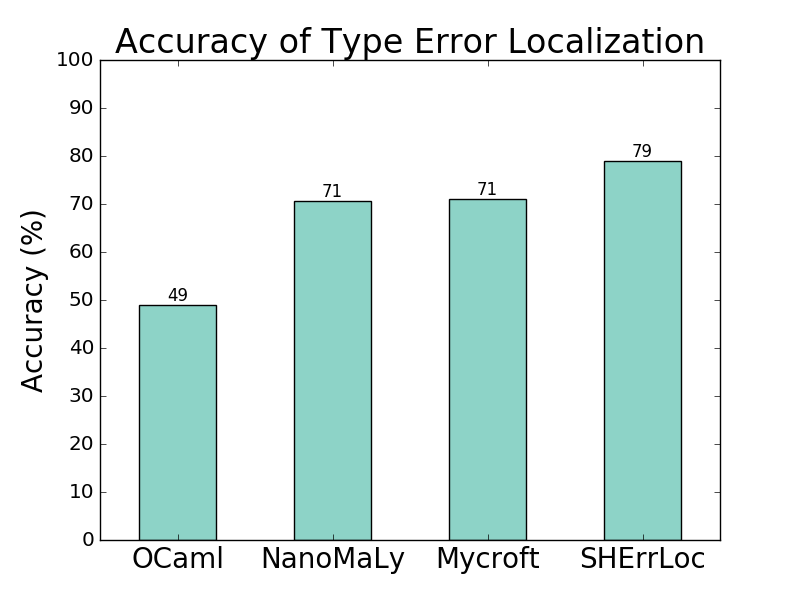
\includegraphics[width=0.7\linewidth]{nanomaly/blame.png}
\caption{Accuracy of type error localization. \toolname's witness-based
  predictions outperform \ocaml by 22 points, and are competitive
  with the state-of-the-art tools \mycroft and \sherrloc.}
\label{fig:results-blame}
\end{figure}

\paragraph{Results}
Figure~\ref{fig:results-blame} summarizes our results, which show that
\toolname's witnesses are competitive with \mycroft and \sherrloc in
automatically locating the source of a type error.
%
\toolname, \mycroft, and \sherrloc all outperform the \ocaml compiler,
which is not surprising given that they can produce multiple possible
error locations, while the \ocaml compiler is limited to one predicted
error location.
%
Interestingly, while all tools have a median of 2 predicted error
locations per program, \mycroft and \sherrloc have a long tail with a
maximum of 22 (\resp 12) locations, while \toolname's maximum is 5
locations.
%
We also note that while \mycroft and \sherrloc were designed
specifically to \emph{localize} type errors, \toolname's foremost
purpose is to \emph{explain} them, we consider its ability to localize
type errors an added benefit.

%%% Local Variables:
%%% mode: latex
%%% TeX-master: "main"
%%% End:


\subsection{Discussion}
\label{sec:nanomaly:discussion}

To summarize, our experiments demonstrate that \nanomaly finds witnesses
to type errors:
%
(1) with high coverage in a timespan amenable to compile-time analysis;
%
(2) with traces that have a low median complexity of 5 jumps;
%
(3) that are more helpful to novice programmers than traditional type
error messages; and
%
(4) that can be used to automatically locate the source of a type error.

There are, of course, drawbacks to our approach. Four that stand out
are:
%
(1) coverage limits due to random generation;
%
(2) dealing with explosions in the size of generated traces;
%
%(3) the inability to handle certain instances of infinite types; and
(3) our use of a non-parametric function type; and
%
(4) handling ad-hoc polymorphism.

\paragraph{Random Generation}
Random test generation has difficulty generating highly constrained
values, \eg\ red-black trees or a pair of equal integers. If the type
error is hidden behind a complex branch condition \nanomaly\ may not be
able to trigger it. Exhaustive testing and dynamic-symbolic execution
can address this short-coming by performing an exhaustive search for
inputs (\emph{resp}.\ paths through the program). As our experiments
show, however, novice programs do not appear to require more advanced
search techniques, likely because they tend to be simple.

% \paragraph{Infinite Types}
% Our implementation does check for infinite types inside \forcesym, but
% there are some degenerate cases where it is unable to detect
% them. Consider the following buggy @replicate@.
% %
% \begin{code}
%   let rec replicate n x =
%     if n <= 0 then
%       []
%     else
%       replicate (n-1) [x]
% \end{code}
% %
% This code produces a nested list (with @n@ levels of nesting) containing
% a single copy of @x@, instead of a list with @n@ copies of @x@. \ocaml\
% detects a cyclic \hbox{@'a = 'a list@} constraint in the recursive call
% and throws a type error, whereas \nanomaly\ happily recurses @n@ times to
% produces the nested list.  Strictly speaking, this function itself cannot
% ``go wrong'', the program would not get stuck until a \emph{client}
% attempted to use the result expecting a flat list. But this is not very
% satisfying as @replicate@ is clearly to blame. Furthermore, in our
% experience, infinite-type errors are often difficult to %some of the more difficult ones to
% debug (and to explain to novices), so better support for this scenario
% would be useful.

\paragraph{Trace Explosion}
Though the average complexity of our generated traces is low in terms of
jumps, there are some extreme outliers.
%
We cannot reasonably expect a novice user to explore a trace containing
50+ terms and draw a conclusion about which pieces contributed to the
bug in their program.
%
Enhancing our visualization to slice out program paths relevant to
specific values~\cite{Perera2012-dy}, would likely help alleviate this
issue, allowing users to highlight a confusing value and ask: ``Where
did this come from?''

\paragraph{Non-Parametric Function Type}
As we discussed in \S~\ref{sec:nanomaly:how-safe} some ill-typed programs
lack a witness in our semantics due to our use of a non-parametric
type $\tfun$ for functions.
%
These programs cannot ``go wrong'', strictly speaking, but would be very
difficult to \emph{use} in practice.
%
We also note that many of these programs induce cyclic typing constraints,
causing infinite-type errors, which in our experience can be particularly
difficult to debug (and to explain to novices).
%
Better support for these programs would be welcome.
%
For example, we might track how the types of inputs change between
recursive calls.
%
If we cannot find a traditional witness, we could then produce a trace
expanded to show these particular steps.

\paragraph{Ad-Hoc Polymorphism}
% Our approach can only support ad-hoc polymorphism (\eg\ type-classes in
% \haskell\ or polymorphic comparison functions in \ocaml) in limited cases
% where we have enough typing information at the call-site to resolve the
% overloading. For example, consider the @n <= 0@ test in our @fac@ example.
% @<=@ is polymorphic in \ocaml, but in this case we can make progress because
% the literal @0@ is not. If we parameterized @fac@ by a lower bound, \eg
% %
% \begin{code}
%   let rec fac n m =
%     if n <= m then
%       1
%     else
%       n * fac (n - 1) m
% \end{code}
% %
% and called @fac@ with two holes, we would get stuck at the @n <= m@
% test; not because of a type error, but because all we know about
% @n@ and @m@ at that point is that they must have the same (unknown)
% type.

Also discussed in \S~\ref{sec:nanomaly:how-safe}, our approach can only support
ad-hoc polymorphism (\eg\ type-classes in \haskell\ or polymorphic
comparison functions in \ocaml) in limited cases where we have enough
typing information at the call-site to resolve the overloading. This
issue is uncommon in \ocaml\ (we detected it in around 5\% of our
benchmarks), but it would surely be exacerbated by a language like
\haskell, which makes heavy use of overloading. We suspect that either
dynamic-symbolic execution or speculative instantiation of holes would
allow us to handle ad-hoc polymorphism, but defer a proper treatment to
future work.

% \begin{itemize}
% \item benchmarks: our data + seminal data
% \item both cases: \textbf{random} search sufficient to trigger runtime crash in 80\% of programs
% \item how many of the ``safe'' programs are actually safe??
% \end{itemize}

%%% Local Variables:
%%% mode: latex
%%% TeX-master: "main"
%%% End:
%!TEX root = main.tex

\section{Related Work}
\label{sec:nanomaly:related-work}
% In this section we connect our work to related efforts on type errors,
% testing, and program exploration.

% \paragraph{Type Errors}
% \label{sec:nanomaly:type-error}

\paragraph{Localizing and Repairing Type Errors}
\label{sec:nanomaly:diagnosis-repair}
% It is well known that
% unification-based type inference procedures can
% produce poor error messages, and in particular, can misidentify the
% \emph{source} of the type error.
%
Many groups have explored techniques to pinpoint the true source
of errors reported by static type checkers.
% unification-based type inference procedures.
%
% \subparagraph{Localization}
The traditional Damas-Milner type inference algorithm~\cite{Damas1982-uw}
reports the first program location where a type mismatch is discovered
(subject to the traversal strategy~\cite{Lee1998-ys}).
%
As a result the error can be reported far away from its
source~\cite{McAdam1998-ub} without enough information to guide the
user.
%
Type-error slicing~\cite{Haack2003-vc,Schilling2011-yf,Rahli2015-tt,Sagonas2013-bf,Gast2004-zd,Neubauer2003-xv}
%treats type inference as a constraint-satisfaction problem and
recognizes this flaw and instead produces a slice of the program
containing \emph{all} program locations that are connected to the type
error.
%
%% \cite{Neubauer2003-xv} present a decidable type system based on
%% discriminative sum types, in which all terms are typeable and type
%% derivations contain all type errors in a program. They then use the
%% typing derivation to slice out the parts of the expression related to
%% each error.
%
Though the program slice must contain the source of the error, it can
suffer from the opposite problem of providing \emph{too much}
information, motivating recent work in ranking the candidate locations.
%
Zhang~\etal~\citealt{Zhang2014-lv,Zhang2015-yu} present an algorithm for
identifying the most likely culprit using Bayesian reasoning.
%
Pavlinovic~\etal~\citealt{Pavlinovic2014-mr,Pavlinovic2015-kh}
translate the %error
localization problem to a MaxSMT optimization problem, using
compiler-provided weights to rank the possible sources.
%
Loncaric~\etal~\citealt{Loncaric2016-uk} improve the scalability of
Pavlinovic~\etal by reusing the existing type checker as
a theory solver in the Nelson-Oppen~\citealt{Nelson1979-td}
style, thus requiring only a MaxSAT solver.

% \subparagraph{Repairing}
In addition to localizing the error, Lerner~\etal~\citealt{Lerner2007-dt} attempt to
suggest a fix by replacing expressions (or removing them entirely) with
alternatives based on the surrounding program context.
%
Chen~\&~Erwig~\citealt{Chen2014-gd} use a variational type system to allow for the
possibility of changing an expression's type, and search for an
expression whose type can be changed such that type inference would
succeed.
%
% It then attempts to deduce the error source by searching for an
% expression whose type can be changed such that type inference would
% succeed.
%
In contrast to Lerner~\etal, who search for changes at the value-level,
Chen~\&~Erwig search at the type-level and are thus complete due the finite
universe of types used in the program.
%
% \item \cite{chen_error-tolerant_2012}
% \item \cite{okeefe_type_1992}
% \item \cite{gomard_partial_1990}
% \item \cite{thatte_type_1988}
%

In contrast to these approaches, we do not attempt to localize or fix
the type error. Instead we try to explain it to the user using a
dynamic witness that demonstrates how the program is not just
ill-typed but truly wrong. In addition, allowing users to run their
program (even knowing that it is wrong)
enables experimentation and the
use of debuggers to step through the program and investigate its
evolution.

\paragraph{Improving Error Messages}
%
The content and quality of the error messages themselves has also been
studied extensively.
%
Marceau~\etal~\citealt{Marceau2011-ok,Marceau2011-cy} study the effectiveness of error
messages in novice environments and present suggestions for improving
their quality and consistency.
%
Hage~\&~Heeren~\citealt{Hage2006-hc} identify a variety of general heuristics to improve
the quality of type error messages, based on their teaching experience.
%
Heeren~\etal~\citealt{Heeren2003-db},
Christiansen~\citealt{Christiansen2014-qc}, and
Serrano~\&~Hage~\citealt{Serrano2016-oo}
provide methods for library authors to specialize
type errors with domain-specific knowledge.
%
The difference with our work is more pronounced here as we do not
attempt to improve the quality of the error message, instead we search
for a witness to the error and explain it with the resulting execution
trace.
%



\paragraph{Running Ill-Typed Programs}
\label{sec:nanomaly:running-ill-typed}
Vytiniotis~\etal~\citealt{Vytiniotis2012-gh} extend the \haskell
compiler GHC to support compiling ill-typed programs, but their intent
is rather different from ours. Their goal was to allow programmers to
incrementally test refactorings, which often cause type errors in
distant functions. They replace any expression that fails to type
check with a \emph{runtime} error, but do not check types
at runtime.
%
Bayne~\etal~\citealt{Bayne2011-cn} also provide a semantics for running
ill-typed (\java) programs, but in constrast transform the program to
perform nearly all type checking at run-time. The key difference between
Bayne~\etal\ and our work is that we use the dynamic semantics to
automatically search for a witness to the type error, while their focus
is on incremental, programmer-driven testing.

\paragraph{Testing}\label{sec:nanomaly:testing}
%
\nanomaly is at its heart a test generator, and as such,
builds on a rich line of work.
%
Our use of holes to represent unknown values is inspired by the work of
Runciman, Naylor, and Lindblad~\cite{Runciman2008-ka,Naylor2007-mi,Lindblad2007-oy},
%
who use lazy evaluation to drastically reduce the search space for
exhaustive test generation, by grouping together equivalent inputs by
the set of values they force. An exhaustive search is complete (up to
the depth bound), if a witness exists it will be found, but due to the
exponential blowup in the search space the depth bound can be quite
limited without advanced grouping and filtering techniques.
%
Our search is not exhaustive; instead we use random generation to fill
in holes on demand.
%
Random test generation~\cite{Claessen2000-lj,Csallner2004-bf,Pacheco2007-at}
%
is by its nature incomplete, but is able to check larger inputs than
exhaustive testing as a result.

Instead of enumerating values, which may trigger the same path through
the program, one might enumerate paths.
%
Dynamic-symbolic execution~\cite{Godefroid2005-am,Cadar2008-kg,Tillmann2008-qc}
%
combines symbolic execution (to track which path a given input triggers)
with concrete execution (to ensure failures are not spurious). The
system collects a path condition during execution, which tracks
symbolically what conditions must be met to trigger the current
path. Upon successfully completing a test run, it negates the path
condition and queries a solver for another set of inputs that satisfy
the negated path condition, \ie inputs that will not trigger the same
path. Thus, it can prune the search space much faster than techniques
based on enumerating values, but is limited by the expressiveness of the
underlying solver.

Our operational semantics is amenable to dynamic-symbolic execution, one
would just need to collect the path condition and replace our
implementation of \gensym by a call to the solver. We chose to use lazy,
random generation instead because it is efficient, does not incur
the overhead of an external solver, and produces high coverage for our
domain of novice programs.

A function's type is a theorem about the its behavior.
Thus, \toolname's witnesses can be viewed as \emph{counter-examples},
thereby connecting it to work on using test cases to find
counter-examples prior to starting a proof~\cite{Chamarthi2011-fo,Seidel2015-pe}.

% \begin{itemize}
% \item \cite{Claessen2000-lj}
% \item
% \item \cite{Godefroid2005-am}
% \item \cite{Cadar2008-kg}
% \item \cite{Tillmann2008-qc}
% \end{itemize}

\paragraph{Program Exploration}

Flanagan~\etal~\citealt{Flanagan1996-bu} describe a static debugger for Scheme, which helps
the programmer interactively visualize problematic source-sink flows
corresponding to soft-typing errors. The debugger allows the user to explore
an abstract reduction graph computed from a static value set analysis of
the program. In contrast, \toolname generates witnesses and allows the user
to explore the resulting dynamic execution.
%
Perera~\etal~\citealt{Perera2012-dy} present a tracing semantics
for functional programs that tags values with their provenance, enabling
a form of backwards program slicing from a final value to the sequence
of reductions that produced it. Notably, they allow the user to supply a
\emph{partial value} --- containing holes --- and present a partial slice,
containing only those steps that affected the the partial value.
% This
% system is designed to answer questions of the form ``Where did this
% value come from?'' and thus is focused on backward exploration.
Perera~\etal\ focus on backward exploration; in contrast, our
visualization supports forward \emph{and} backward exploration, though
our backward steps are more limited.
%
Specifically, we do not support selecting a value and inserting the
intermediate terms that preceded it while ignoring unrelated computation
steps. %; this would be interesting future work.

% \ES{todo: more on program exploration}

%%% Local Variables:
%%% mode: latex
%%% TeX-master: "../main"
%%% End:

\lstDeleteShortInline{@}

%\chapter{Type Targeted Testing}
%\lstMakeShortInline{@}
%\renewcommand\toolname{\tool{Target}}
%\section{Introduction}\label{sec:intro}

Should the programmer spend her time writing \emph{better types}
or \emph{thorough tests}?  
%
Types have long been the most pervasive means of describing the 
intended behavior of code. However, a type signature is often a 
very coarse description; the actual inputs and outputs
may be a subset of the values described by the types. 
%
For example, the set of ordered integer lists is a very 
sparse subset of the set of all integer lists. 
%
Thus, to validate functions that produce or consume such values, 
the programmer must painstakingly enumerate these values by hand 
or via ad-hoc generators for unit tests.

We present a new technique called \emph{type targeted testing}, 
abbreviated to \toolname, that enables the generation of unit
tests from precise \emph{refinement types}.
%
Over the last decade, various groups have shown how refinement 
types -- which compose the usual types with logical refinement predicates
that characterize the subset of actual type inhabitants -- 
can be used to specify and formally verify a wide variety 
of correctness properties of programs~\cite{pfenningxi98,Dunfield07,fstar,VazouICFP14}.
%
Our insight is that through the lens of SMT
solvers, refinement types can be viewed as a high-level, 
declarative, test generation technique.

\toolname tests an implementation function against a refinement 
type specification using a \emph{query-decode-check} loop.
%
% NV: input implies the types TARGET gets as input
First, \toolname translates the argument types into a logical
\emph{query} for which we obtain a satisfying assignment 
(or model) from the SMT solver.
%
Next, \toolname \emph{decodes} the SMT solver's model to obtain
concrete input values for the function.
%
Finally, \toolname executes the function on the inputs 
to get the corresponding output, which we \emph{check} 
belongs to the specified result type. 
%
If the check fails, the inputs are returned as a counterexample, 
otherwise
%
\toolname refutes the given model to force the SMT solver to 
return a different set of inputs. 
%
This process is repeated for a given number of 
iterations, or until \emph{all} inputs up to a certain size 
have been tested.

% Vs. Testing
\toolname offers several benefits over other testing techniques.
%
Refinement types provide a succinct description of the 
input and output requirements, eliminating the need to 
enumerate individual test cases by hand or to write 
custom generators.
%
Furthermore, \toolname generates \emph{all} 
values (up to a given size) that inhabit a type, and thus
does not skip any corner cases that a hand-written generator 
might miss.
%
Finally, while the above advantages can be recovered by a brute-force
generate-and-filter approach that discards inputs that do not meet
some predicate, we show that our SMT-based method can be significantly
more efficient for enumerating valid inputs in a highly-constrained space.
% and hence, sparse space.

% Vs. Verification 
\toolname paves a \emph{gradual path} from testing to verification, 
that affords several advantages over verification.
%
First, the programmer has an \emph{incentive} to write formal 
specifications using refinement types. \toolname provides the 
immediate gratification of an automatically generated, 
exhaustive suite of unit tests that can expose errors.
Thus, the programmer is rewarded without paying, up front, 
the extra price of annotations, hints, strengthened 
inductive invariants, or tactics needed for formally 
verifying the specification.
%
Second, our approach makes it possible to use refinement 
types to formally verify \emph{some} parts of the program, 
while using tests to validate other parts that may
be too difficult to verify
%
\toolname integrates the two modes by using refinement
types as the uniform specification mechanism. 
Functions in the verified half can be formally checked 
\emph{assuming} the functions in the tested half adhere 
to their specifications. 
We could even use refinements to generate dynamic 
contracts~\cite{Findler01} around the tested half 
if so desired.
%
Third, even when formally verifying the type specifications, 
the generated tests can act as valuable \emph{counterexamples} 
to help \emph{debug} the specification or implementation in 
the event that the program is rejected by the verifier.

% Vs. SymEx 
Finally, \toolname offers several concrete advantages over previous
property-based testing techniques, which also have the potential for 
gradual verification.
%
First, instead of specifying properties with arbitrary code 
\cite{claessen_quickcheck:_2000,runciman_smallcheck_2008} 
which complicates the task of subsequent formal verification, 
with \toolname the properties are specified via refinement 
types, for which there are already several existing formal 
verification algorithms~\cite{VazouICFP14}.
%
Second, while symbolic execution tools~\cite{DART,CUTE,Veanes08} 
can generate tests from arbitrary code contracts (\eg assertions) 
we find that highly constrained inputs trigger path explosion 
which precludes the use of such tools for gradual verification.

% In the rest of the paper...
In the rest of this paper, we start with an overview of 
how \toolname can be used and how its query-decode-check 
loop is implemented (\S~\ref{sec:overview}).
%
Next, we formalize a general framework for type-targeted 
testing (\S~\ref{sec:framework}) and show how it can be 
instantiated to generating tests for lists (\S~\ref{sec:list}), 
and then automatically generalized to other 
types (\S~\ref{sec:generic}).
%
All the benefits of \toolname come at a price; 
we are limited to properties that can be specified with 
refinement types. 
%
We present an empirical evaluation that shows
\toolname is efficient and expressive enough to capture 
a variety of sophisticated properties,
%
demonstrating that type-targeted 
testing is
a sweet spot between automatic testing 
and verification (\S~\ref{sec:evaluation}).

%%% Second, \toolname's symbolic, SMT-based approach makes it possible
%%% to systematically generate values that satisfy highly constrained 
%%% pre-conditions which otherwise thwart the generate-and-filter 
%%% approach of traditional property-based tools.
%%% %
%%% While this work shows a great deal of promise for making 
%%% formal verification practical, it does not obviate the 
%%% need for testing.
%%% %
%%% First, it can take a great deal of effort and expertise 
%%% to write down the annotations (beyond the end-to-end 
%%% specification) needed to verify a program 
%%% %
%%% Second, there maybe requirements (\eg performance) that 
%%% are not easily specified via refinements.
%%% ES INTRO We present \toolname, an automatic test-generator that uses SMT-solvers 
%%% ES INTRO to generate test-cases, taking advantange of their efficient decision 
%%% ES INTRO procedures to quickly prune the search space of all inputs. 
%%% ES INTRO 
%%% ES INTRO We observe based on prior work that many interesting properties of
%%% ES INTRO functions can be specified in an SMT-decidable logic, in our case the
%%% ES INTRO logic of linear arithetic, equality, and uninterpreted functions
%%% ES INTRO (\smtlogic).
%%% ES INTRO 
%%% ES INTRO Building on top of the \liquidhaskell program verification
%%% ES INTRO tool~\cite{VazouRealWorld14}, we show how a single data generator can
%%% ES INTRO be used to produce values of a type that satisfy disparate
%%% ES INTRO constraints, thereby easing the tedium of testing
%%% ES INTRO (\S~\ref{sec:liquidcheck}). 
%%% ES INTRO 
%%% ES INTRO We further show how to use a single generator to generically produce
%%% ES INTRO values of \emph{any} algebraic datatype (\S~\ref{sec:generic-generation}). 
%%% ES INTRO 
%%% ES INTRO Finally, we note that due to our shared specification language with
%%% ES INTRO \liquidhaskell, our properties are immediately ammenable to formal
%%% ES INTRO verification, should the developer wish to invest the extra time
%%% ES INTRO (\S~\ref{sec:discussion}).

%\section{Overview}\label{sec:overview}

We start with a series of examples pertaining to a small grading
library called @Scores@. The examples provide a bird's eye view of 
how a user interacts with \toolname, how \toolname is implemented,
and the advantages of type-based testing.

\mypara{Refinement Types}
A refinement type is one where the basic types are decorated 
with logical predicates drawn from an efficiently decidable 
theory. For example,
%
\begin{code}
  type Nat   = {v:Int | 0 <= v}
  type Pos   = {v:Int | 0 <  v}
  type Rng N = {v:Int | 0 <= v && v <  N}
\end{code}
%
are refinement types describing the set of integers that are 
non-negative, strictly positive, and in the interval @[0, N)@ 
respectively. We will also build up function and collection 
types over base refinement types like the above. 
%
In this paper, we will not address the issue of \emph{checking}
refinement type signatures~\cite{VazouICFP14}.
%
We assume the code is typechecked, \eg by GHC, against the 
standard type signatures obtained by erasing the refinements.
Instead, we focus on using the refinements to 
synthesize tests to \emph{execute} the function, and to find 
\emph{counterexamples} that violate %demonstrate the function does not meet
the given specification.

\subsection{Testing with Types}

\mypara{Base Types}
Let us write a function @rescale@ that takes a source range @[0,r1)@, 
a target range @[0,r2)@, and a score @n@ from the source range,
and returns the linearly scaled score in the target range.
%
For example, @rescale 5 100 2@ should return @40@. 
Here is a first attempt at @rescale@ 
%
\begin{code}
  rescale :: r1:Nat -> r2:Nat -> s:Rng r1 -> Rng r2 
  rescale r1 r2 s = s * (r2 `div` r1)   
\end{code}
%
When we run \toolname, it immediately reports 
%
\begin{code}
  Found counter-example: (1, 0, 0) 
\end{code}
%
Indeed, @rescale 1 0 0@ results in @0@ which is not in the target 
@Rng 0@, as the latter is empty! We could fix this in various ways, 
\eg by requiring the ranges are non-empty:
%
\begin{code}
  rescale :: r1:Pos -> r2:Pos -> s:Rng r1 -> Rng r2 
\end{code}
%
Now, \toolname accepts the function and reports
%
\begin{code}
  OK. Passed all tests.
\end{code}
%
Thus, using the refinement type \emph{specification} for @rescale@, 
\toolname systematically tests the \emph{implementation} by generating 
all valid inputs (up to a given size bound) that respect the 
pre-conditions, running the function, and checking that the 
output satisfies the post-condition.
%
Testing against random, unconstrained inputs would be of limited value 
as the function is not designed to work on all @Int@ values. While in 
this case we could filter invalid inputs, we shall show
that \toolname can be more effective.

\mypara{Containers}
Let us suppose we have normalized all scores to be out of @100@
%
\begin{code}
  type Score = Rng 100
\end{code}
%
Next, let us write a function to compute a \emph{weighted} average 
of a list of scores.
%
\begin{code}
  average     :: [(Int, Score)] -> Score
  average []  = 0
  average wxs = total `div` n
    where
      total   = sum [w * x | (w, x) <- wxs ]
      n       = sum [w     | (w, _) <- wxs ]
\end{code}
%
It can be tricky to \emph{verify} this function as it requires non-linear reasoning
about an unbounded collection. However, we can gain a great degree of confidence by
systematically testing it using the type specification; indeed, \toolname responds:
%
\begin{code}
  Found counter-example: [(0,0)]
\end{code}
%
Clearly, an unfortunate choice of weights can trigger a divide-by-zero; we can fix 
this by requiring the weights be non-zero:
%
\begin{code}
  average :: [({v:Int | v /= 0}, Score)] -> Score
\end{code}
%
but now \toolname responds with
%
\begin{code}
  Found counter-example: [(-3,3),(3,0)]
\end{code}
% 
which also triggers the divide-by-zero! We will play it safe and require positive weights,
%
\begin{code}
  average :: [(Pos, Score)] -> Score
\end{code}
%
at which point \toolname reports that all tests pass.

\mypara{Ordered Containers}
The very nature of our business requires that at the end of the day,
we order students by their scores. We can represent ordered lists by 
requiring the elements of the tail @t@ to be greater than the head @h@:
%
\begin{code}
data OrdList a = [] | (:) {h :: a, t :: OrdList {v:a | h <= v}}
\end{code}
%
Note that erasing the refinement predicates gives us plain old Haskell lists.
We can now write a function to insert a score into an ordered list:
%
\begin{code}
  insert :: (Ord a) => a -> OrdList a -> OrdList a 
\end{code}
%
\toolname automatically generates all ordered lists (up to a given size)
and executes @insert@ to check for any errors. Unlike randomized testers, 
\toolname is not thwarted by the ordering constraint, and does not require a
custom generator from the user.

\mypara{Structured Containers} 
Everyone has a few bad days. Let us write a function that takes the 
@best k@ scores for a particular student. That is, the output
must satisfy a \emph{structural} constraint -- that its size 
equals @k@. We can encode the size of a list with a logical 
measure function~\cite{VazouICFP14}:
%
\begin{code}
  measure len :: [a] -> Nat
  len []      = 0
  len (x:xs)  = 1 + len xs
\end{code}
%
Now, we can stipulate that the output indeed has @k@ scores:
%
\begin{code}
  best      :: k:Nat -> [Score] -> {v:[Score] | k = len v}
  best k xs = take k $ reverse $ sort xs
\end{code}
%
Now, \toolname quickly finds a counterexample:
%
\begin{code}
  Found counter-example: (2,[])
\end{code}
%
Of course -- we need to have at least @k@ scores to start with! 
%
\begin{code}
best :: k:Nat -> {v:[Score]|k <= len v} -> {v:[Score]|k = len v}
\end{code}
%
and now, \toolname is assuaged and reports no counterexamples.
%
While randomized testing would suffice for @best@, we will see 
more sophisticated structural properties such as height balancedness, 
which stymie random testers, but are easily handled by \toolname.

\mypara{Higher-order Functions} 
Perhaps instead of taking the $k$ best grades, we would like
to pad each individual grade, and, furthermore, we want to
be able to experiment with different padding functions. Let
us rewrite @average@ to take a functional argument, and
stipulate that it can only increase a @Score@.
%
\begin{code}
  padAverage       :: (s:Score -> {v:Score | s <= v}) 
                   -> [(Pos, Score)] -> Score
  padAverage f []  = f 0
  padAverage f wxs = total `div` n
    where
      total   = sum [w * f x | (w, x) <- wxs ]
      n       = sum [w       | (w, _) <- wxs ]
\end{code}
%
\toolname automatically checks that @padAverage@ is 
a safe generalization of @average@. Randomized 
testing tools can also generate functions, but those 
functions are unlikely to satisfy non-trivial constraints, 
thereby burdening the user with custom generators.


\subsection{Synthesizing Tests} 
\label{sec:synthesizing-tests}
Next, let us look under the hood to get an idea of how \toolname 
synthesizes tests from types. 
% INTRO
At a high-level, our strategy is to:
%
(1)~\emph{query}   an SMT solver for satisfying assigments to a set of logical 
                   constraints derived from the refinement type,
(2)~\emph{decode}  the model into Haskell values that are suitable inputs,
(3)~\emph{execute} the function on the decoded values to obtain the output, 
(4)~\emph{check}   that the output satisfies the output type,
(5)~\emph{refute}  the model to generate a different test, and 
repeat the above steps until all tests up to a certain size are executed.
%
We focus here on steps 1, 2, and 4 -- query, decode, and check -- the others are 
standard and require little explanation.

\mypara{Base Types}
Recall the initial (buggy) specification
%
\begin{code}
  rescale :: r1:Nat -> r2:Nat -> s:Rng r1 -> Rng r2 
\end{code}
%
\toolname \emph{encodes} input requirements for base types directly 
from their corresponding refinements. The constraints for multiple, 
related inputs are just the \emph{conjunction} of the constraints 
for each input. Hence, the constraint for @rescale@ is:
%
$$
\cstr{C_0} \defeq 0 \leq \cvar{r1} \wedge 0 \leq \cvar{r2} \wedge 0 \leq s < \cvar{r1} 
$$
%
In practice, $\cstr{C_0}$ will also contain conjuncts of the form $-N \leq x \leq N$ that
restrict @Int@-valued variables $x$ to be within the size bound $N$ supplied by
the user, but we will omit these throughout the paper for clarity.
%% %
%% For clarity, we omit the conjuncts of the form $-N \leq x \leq N$
%% that restrict @Int@-valued variables $x$ to be within the size
%% bound $N$ supplied by the user.

Note how easy it is to capture dependencies between inputs, 
\eg that the score @s@ be in the range defined by @r1@.
%
On querying the SMT solver with the above, we get a model
%
$[\cvar{r1} \mapsto 1, \cvar{r2} \mapsto 1, \cvar{s}  \mapsto 0]$.
%
\toolname decodes this model and executes \hbox{@rescale 1 1 0@} to obtain the value @v = 0@.
%
Then, \toolname validates @v@ against the post-condition by checking 
% that it inhabits the output type, \ie by checking 
the validity of the output type's constraint: 
%
$$\cvar{r2} = 1 \wedge \cvar{v} = 0 \wedge 0 \leq \cvar{v} \wedge \cvar{v} < \cvar{r2}$$
%
As the above is valid, \toolname moves on to generate another 
test by conjoining $\cstr{C_0}$ with a constraint that refutes 
the previous model:
%
$$
\cstr{C_1} \defeq \cstr{C_0} \wedge (\cvar{r1} \not = 1 \vee \cvar{r2} \not = 1 \vee \cvar{s} \not = 0)
$$
This time, the SMT solver returns a model: 
%
$[\cvar{r1} \mapsto 1, \cvar{r2} \mapsto 0, \cvar{s} \mapsto 0]$
%
which, when decoded and executed, yields the result $0$ that does \emph{not} 
inhabit the output type, and so is reported as a counterexample. 
%
When we fix the specification to only allow @Pos@ ranges, each test produces
a valid output, so \toolname reports that all tests pass.

\mypara{Containers}
Next, we use \toolname to test the implementation of @average@.
To do so, \toolname needs to generate Haskell lists with the appropriate constraints.
%
Since each list is recursively 
either ``nil'' 
or ``cons'', 
\toolname generates constraints that symbolically 
represent \emph{all} possible lists up to a given depth, 
using propositional \emph{choice variables} to 
symbolically pick between these two alternatives.
%
Every (satisfying) assignment of choices returned by 
the SMT solver gives \toolname the concrete data and 
constructors used at each level, allowing it to decode 
the assignment into a Haskell value.

For example, \toolname represents valid @[(Pos, Score)]@ 
inputs (of depth up to 3), required to test @average@, 
as the conjunction of $\cstr{C_{list}}$ and $\cstr{C_{data}}$:
%
\begin{eqnarray*}
\cstr{C_{list}} & \defeq & (\cvar{c}_{00} \Rightarrow \cvar{xs}_0 = \lnil) \wedge 
                          (\cvar{c}_{01} \Rightarrow \cvar{xs}_0 = \lcons{\cvar{x}_1}{\cvar{xs}_1}) \wedge 
                          (\cvar{c}_{00} \oplus \cvar{c}_{01}) \\
               & \wedge & (\cvar{c}_{10} \Rightarrow \cvar{xs}_1 = \lnil) \wedge
                          (\cvar{c}_{11} \Rightarrow \cvar{xs}_1 = \lcons{\cvar{x}_2}{\cvar{xs}_2}) \wedge 
                          (\cvar{c}_{01} \Rightarrow \cvar{c}_{10} \oplus \cvar{c}_{11}) \\
               & \wedge & (\cvar{c}_{20} \Rightarrow \cvar{xs}_2 = \lnil) \wedge 
                          (\cvar{c}_{21} \Rightarrow \cvar{xs}_2 = \lcons{\cvar{x}_3}{\cvar{xs}_3}) \wedge 
                          (\cvar{c}_{11} \Rightarrow \cvar{c}_{20} \oplus \cvar{c}_{21}) \\
               & \wedge & (\cvar{c}_{30} \Rightarrow \cvar{xs}_3 = \lnil) \wedge 
                          (\cvar{c}_{21} \Rightarrow \cvar{c}_{30}) \\[0.1in]
\cstr{C_{data}} & \defeq & (\cvar{c}_{01} \Rightarrow \cvar{x}_1 = \ltup{\cvar{w}_1}{\cvar{s}_1} \ \wedge\ 0 < \cvar{w}_1 \ \wedge\ 0 \leq \cvar{s}_1 < 100) \\
               & \wedge & (\cvar{c}_{11} \Rightarrow \cvar{x}_2 = \ltup{\cvar{w}_2}{\cvar{s}_2} \ \wedge\ 0 < \cvar{w}_2 \ \wedge\ 0 \leq \cvar{s}_2 < 100) \\
               & \wedge & (\cvar{c}_{21} \Rightarrow \cvar{x}_3 = \ltup{\cvar{w}_3}{\cvar{s}_3} \ \wedge\ 0 < \cvar{w}_3 \ \wedge\ 0 \leq \cvar{s}_3 < 100)
\end{eqnarray*}
%
The first set of constraints $\cstr{C_{list}}$ describes all lists up to 
size 3. At each level $i$, the \emph{choice} variables $\cvar{c}_{i0}$ 
and $\cvar{c}_{i1}$ determine whether at that level the constructed 
list $\cvar{xs}_i$ is a ``nil'' or a ``cons''. 
%
In the constraints $\lnil$ and $(\lcons{}{})$ are \emph{uninterpreted} 
functions that represent ``nil'' and ``cons'' respectively. 
These functions only obey the congruence axiom and hence, can be 
efficiently analyzed by SMT solvers~\cite{Nelson81}.
%
The data at each level $\cvar{x}_i$ is constrained to be a pair of a 
positive weight $\cvar{w}_i$ and a valid score $\cvar{s}_i$.

The choice variables at each level are used to \emph{guard} the 
constraints on the next levels. 
%
First, if we are generating a ``cons'' at a given level, then
exactly one of the choice variables for the next level must be 
selected;
\eg  $\cvar{c}_{11} \Rightarrow \cvar{c}_{20} \oplus \cvar{c}_{21}$.
%
Second, the constraints on the data at a given level only hold 
if we are generating values for that level; \eg $\cvar{c}_{21}$ 
is used to guard the constraints on $\cvar{x}_3$, $\cvar{w}_3$ 
and $\cvar{s}_3$.
%
This is essential to avoid over-constraining the system 
which would cause \toolname to miss certain tests.

To \emph{decode} a model of the above into a Haskell value of type @[(Int, Int)]@,
we traverse constraints and use the valuations of the choice variables to 
build up the list appropriately.
%
At each level, if $\cvar{c}_{i0} \mapsto \ttrue$, then the list at that 
level is @[]@, otherwise $\cvar{c}_{i1} \mapsto \ttrue$ and we decode 
$\cvar{x}_{i+1}$ and $\cvar{xs}_{i+1}$ and ``cons'' the results.

We can iteratively generate \emph{multiple} inputs by adding a constraint that
refutes each prior model. As an important optimization, we only refute the
relevant parts of the model, \ie those needed to construct the list
(\S~\ref{sec:refute}).

\mypara{Ordered Containers}
%
Next, let us see how \toolname enables automatic testing with 
highly constrained inputs, such as the \emph{increasingly ordered} 
@OrdList@ values required by @insert@.
%
From the type definition, it is apparent that ordered
lists are the same as the usual lists described by
$\cstr{C_{list}}$, except that each unfolded \emph{tail} 
must only contain values that are greater than the 
corresponding \emph{head}.
%
That is, as we unfold @x1:x2:xs :: OrdList@ 
%
\begin{itemize}
\item At level @0@, we have @OrdList {v:Score| true}@
\item At level @1@, we have @OrdList {v:Score| x1 <= v}@
\item At level @2@, we have @OrdList {v:Score| x2 <= v && x1 <= v}@
\end{itemize}
%
and so on. Thus, we encode @OrdList Score@ (of depth up to 3) by
conjoining $\cstr{C_{list}}$ with  $\cstr{C_{score}}$ and $\cstr{C_{ord}}$,
which capture the valid score and ordering requirements respectively:
%
\begin{eqnarray*}
\cstr{C_{ord}}   & \defeq & (\cvar{c}_{11} \Rightarrow \cvar{x}_1 \leq \cvar{x}_2)
                \ \wedge\  (\cvar{c}_{21} \Rightarrow \cvar{x}_2 \leq \cvar{x}_3\ \wedge\ \cvar{x}_1 \leq \cvar{x}_3) \\[0.01in]
\cstr{C_{score}} & \defeq & (\cvar{c}_{01} \Rightarrow 0 \leq \cvar{x}_1 < 100)
                \ \wedge\  (\cvar{c}_{11} \Rightarrow 0 \leq \cvar{x}_2 < 100)
                \ \wedge\  (\cvar{c}_{21} \Rightarrow 0 \leq \cvar{x}_3 < 100)
\end{eqnarray*}

\mypara{Structured Containers}
Recall that @best k@ requires inputs whose \emph{structure} is constrained -- the 
size of the list should be no less than @k@. We specify size using special measure 
functions~\cite{VazouICFP14}, which let us relate the size of a list with that of
its unfolding, and hence, let us encode the notion of size inside the constraints:
%
\begin{eqnarray*}
\cstr{C_{size}} & \defeq & (\cvar{c}_{00} \Rightarrow \clen{\cvar{xs}_{0}} = 0) \wedge 
                          (\cvar{c}_{01} \Rightarrow \clen{\cvar{xs}_{0}} = 1 + \clen{\cvar{xs}_1}) \\
               & \wedge & (\cvar{c}_{10} \Rightarrow \clen{\cvar{xs}_{1}} = 0) \wedge 
                          (\cvar{c}_{11} \Rightarrow \clen{\cvar{xs}_{1}} = 1 + \clen{\cvar{xs}_2}) \\
               & \wedge & (\cvar{c}_{20} \Rightarrow \clen{\cvar{xs}_{2}} = 0) \wedge 
                          (\cvar{c}_{21} \Rightarrow \clen{\cvar{xs}_{2}} = 1 + \clen{\cvar{xs}_3}) \\
               & \wedge & (\cvar{c}_{30} \Rightarrow \clen{\cvar{xs}_{3}} = 0)
\end{eqnarray*}
%
At each unfolding, we instantiate the definition of the measure 
for each alternative of the datatype. 
%
In the constraints, $\clen{\cdot}$ is an uninterpreted function derived
from the measure definition. All of the relevant properties of the function
are spelled out by the unfolded constraints in $\cstr{C_{size}}$ and hence,
we can use SMT to search for models for the above constraint.
%
Hence, \toolname constrains the input type for @best@ as:
%
$$     0 \leq k 
\wedge \cstr{C_{list}} 
\wedge \cstr{C_{score}} 
\wedge \cstr{C_{size}} 
\wedge k \leq \clen{\cvar{xs}_0} $$
%
where the final conjunct comes from the top-level refinement that 
stipulates the input have at least @k@ scores.
%
Thus, \toolname only generates lists that are large enough. 
For example, in any model where $k = 2$, it will \emph{not} 
generate the empty or singleton list, as in those cases, 
$\clen{\cvar{xs}_0}$ would be $0$ (resp. $1$), violating the 
final conjunct above.

\mypara{Higher-order Functions}
Finally, \toolname's type-directed testing scales up to higher-order
functions using the same insight as in QuickCheck~\cite{claessen_quickcheck:_2000}, namely, 
to generate a function it suffices to be able to 
generate the \emph{output} of the function.
When tasked with the generation of a functional argument @f@, \toolname 
returns a Haskell function that when executed checks
whether its inputs satisfy @f@'s pre-conditions.
If they do, then @f@ uses \toolname to dynamically
query the SMT solver for an output that satisfies the 
constraints imposed by the concrete inputs.
Otherwise, @f@'s specifications are violated
and TARGET reports a counterexample.

This concludes our high-level tour of the benefits and 
implementation of \toolname. 
%
Notice that the property specification mechanism -- 
refinement types -- allowed us to get immediate feedback
that helped debug not just the code, but also the specification 
itself. 
%
Additionally, the specifications gave us machine-readable 
documentation about the behavior of functions, and a large 
unit test suite with which to automatically validate the 
implementation.
%
Finally, though we do not focus on it here, the specifications 
are amenable to formal verification should the programmer 
so desire.


%%% Local Variables:
%%% mode: latex
%%% TeX-master: "main"
%%% End:

%\section{A Framework for Type Targeted Testing}\label{sec:framework}

Next, we describe a framework for type targeted testing, by formalizing
an abstract representation of refinement types~(\S~\ref{sec:reftypes}), 
describing the operations needed to generate tests from types~(\S~\ref{sec:targetable}), 
and then using the above to implement \toolname via a query-decode-check 
loop~(\S~\ref{sec:loop}). 
%
Subsequently, we instantiate the framework to obtain tests
for refined primitive types, lists, algebraic datatypes and higher-order 
functions~(\S~\ref{sec:list}).

%% Next, we describe an (abstract) representation of refinement types,
%% and show how to use them to implement the @query@, @decode@ and @check@ 
%% steps from Figure~\ref{fig:arch}.
 
\subsection{Refinement Types}\label{sec:reftypes}

\begin{figure}[t!]
\begin{mdframed}
\begin{CenteredBox}
\begin{code}
-- Manipulating Refinements
refinement :: RefType -> Refinement
subst      :: RefType -> [(Var, Var)] -> RefType

-- Manipulating Types
unfold     :: Ctor  -> RefType -> [(Var, RefType)]
binder     :: RefType -> Var
proxy      :: RefType -> Proxy a 
\end{code}
\end{CenteredBox}
\end{mdframed}
\caption{Refinement Type API}\label{fig:rtype}
\end{figure}

A refinement type is a type, where each component is 
decorated with a predicate from a refinement logic. 
%
For clarity, we describe refinement types and refinements 
abstractly as @RefType@ and @Refinement@ respectively.
%
We write @Var@ as an alias for @Refinement@ that is 
typically used to represent logical variables appearing
within the refinement.

\mypara{Notation} 
In the sequel, we will use % backticks
double brackets $\meta{}$ to represent the 
various entities in the meta-language used to describe \toolname. 
%
For example, 
|$\meta{k}$|,
|$\meta{k \leq len\ v}$|, and
|$\meta{\reft{v}{[Score]}{k \leq len\ v}}$|
% \hbox{@`{v:[Score] | x0 <= len v}`@}
are the @Var@, @Refinement@, and @RefType@
representing the corresponding entities written in the brackets.


Next, we describe the various operations over them 
needed to implement \toolname.
These operations, summarized in Figure~\ref{fig:rtype}, 
fall into two categories: those which manipulate the 
\emph{refinements} and those which manipulate the 
\emph{types}.

\mypara{Operating on Refinements} 
To generate constraints and check inhabitation, we use 
the function @refinement@ which returns the (top-level) refinement
that decorates the given refinement type.
%
We will generate fresh @Var@s to name values of components, and will 
use @subst@ to replace the free occurrences of variables in a given \hbox{@RefType@.}
%
Suppose that @t@ is the @RefType@ represented by
\hbox{|$\meta{\reft{v}{[Score]}{k \leq len\ v}}$|.} Then,
%
\begin{itemize}
\item{@refinement t@} evaluates to |$\meta{k \leq len\ v}$| and
\item{|subst t [($\meta{k}$, $\meta{x_0}$)]|} evaluates to |$\meta{\reft{v}{[Score]}{x_0 \leq len\ v}}$|.
\end{itemize}

\mypara{Operating on Types} 
To build up compound values (\eg lists) from components 
(\eg an integer and a list), 
%
@unfold@ breaks a @RefType@ (\eg a list of integers) into its 
constituents (\eg an integer and a list of integers) at a given 
constructor (\eg ``cons'').
%
@binder@ simply extracts the @Var@ representing the
value being refined from the \hbox{@RefType@.}
%
To write generic functions over @RefType@s and use Haskell's
type class machinery to @query@ and @decode@ components of
types, we associate with each refinement type a \emph{proxy}
representing the corresponding Haskell type (in practice
this must be passed around as a separate argument).
%
For example, if @t@ is \hbox{|$\meta{\reft{v}{[Score]}{k \leq len\ v}}$|,} 
%
\begin{itemize}
\item{|unfold $\meta{:}$ t|} evaluates to |[($\meta{x}$, $\meta{Score}$), ($\meta{xs}$, $\meta{[Score]}$)]|,
\item{@binder t@} evaluates to |$\meta{v}$|, and
\item{@proxy t@} evaluates to a value of type @Proxy [Int]@.
\end{itemize}

\subsection{The \texttt{Targetable} Type Class}\label{sec:targetable}

% query  :: Haskell-Logic -> Gen SMT-Logic
% decode :: SMT-Value     -> Haskell-Value
% encode :: Haskell-Value -> SMT-Logic 

Following \quickcheck, we encapsulate the key operations needed
for type-targeted testing in a type class @Targetable@ 
(Figure~\ref{fig:targetable}). 
%
\begin{figure}
\begin{mdframed}
\begin{CenteredBox}
\begin{code}
class Targetable a where
  query  :: Proxy a -> Int -> RefType -> SMT Var
  decode :: Var -> SMT a
  check  :: a -> RefType -> SMT (Bool, Var)
  toReft :: a -> Refinement
\end{code}
\end{CenteredBox}
\end{mdframed}
\caption{The class of types that can be tested by \toolname}\label{fig:targetable}
\end{figure}
%
This class characterizes the set of types which can be tested 
by \toolname. All of the operations can interact with an external SMT 
solver, and so return values in an @SMT@ monad.

\begin{itemize}
\item{@query@} takes a \emph{proxy} for the Haskell type
   for which we are generating values, an integer 
   \emph{depth} bound, and a \emph{refinement type}
   describing the desired constraints, and generates a set of 
   logical constraints and a @Var@ that represents the 
   constrained value.

\item{@decode@} takes a @Var@, generated via a previous 
   @query@ and queries the model returned by the SMT solver
   to construct a Haskell value of type @a@.
 
\item{@check@} takes a value of type @a@, translates 
   it back into logical form, and verifies that it inhabits
   the output type @t@.
   
\item{@toReft@} takes a value of type @a@ and translates it
   back into logical form (a specialization of @check@).
\end{itemize}

\subsection{The Query-Decode-Check Loop}\label{sec:loop}



Figure~\ref{fig:arch} summarizes the overall implementation of 
\toolname, which takes as input a function @f@ and its refinement 
type specification @t@ and proceeds to test the function against 
the specification via a \emph{query-decode-check} loop:
%
(1) First, we translate the refined @inputTypes@ into a logical \emph{query}.
%
(2) Next, we \emph{decode} the model (\ie satisfying assignment) for the 
    query returned by the SMT solver to obtain concrete @inputs@.
%
(3) Finally, we @execute@ the function @f@ on the @inputs@ to get the 
    corresponding @output@, which we @check@ belongs to the specified 
    @outputType@. If the @check@ fails, we return the @inputs@ as a counterexample.
%
After each test, \toolname, refutes the given test to force the SMT 
solver to return a different set of inputs, and this process is repeated until 
a user specified number of iterations. The @checkSMT@ call may fail
to find a model meaning that we have exhaustively tested all inputs upto
a given @testDepth@ bound. If all iterations succeed, \ie no counterexamples
are found, then \toolname returns @Ok@, indicating that @f@ satisfies @t@ 
up to the given depth bound.

\begin{figure}[ht!]
\begin{mdframed}
\begin{CenteredBox}
\begin{code} 
target f t = do 
  let txs = inputTypes t
  vars  <- forM txs $ \tx -> 
             query (proxy tx) testDepth tx -- Query
  forM [1 .. testNum] $ \_ -> do
    hasModel <- checkSMT 
    when hasModel $ do
      inputs <- forM vars decode           -- Decode
      output <- execute f inputs                        
      let su = zip (map binder txs) (map toReft inputs)
      let to = outputType t `subst` su
      (ok,_) <- check output to            -- Check
      if ok then 
        refuteSMT 
      else 
        throw (CounterExample inputs)     
  return Ok
\end{code}
\end{CenteredBox}
\end{mdframed}
\caption{Implementing \toolname via a \emph{query-decode-check} loop}\label{fig:arch}
\end{figure}

%\section{Instantiating the \toolname Framework}\label{sec:list}

Next, we describe a concrete instantiation of \toolname for lists.
%
We start with a constraint generation API~(\S~\ref{sec:constraint}). 
%
Then we use the API to implement the key operations 
\hbox{@query@~(\S~\ref{sec:query}),} 
\hbox{@decode@~(\S~\ref{sec:decode}),} 
\hbox{@check@~(\S~\ref{sec:check}),} and
\hbox{@refuteSMT@~(\S~\ref{sec:refute}),} 
thereby enabling \toolname to automatically test functions over lists.
We omit the definition of @toReft@ as it follows directly from the
definition of @check@.
%
Finally, we show how the list instance can be generalized to algebraic 
datatypes and higher-order functions~(\S~\ref{sec:generic}).

\subsection{SMT Solver Interface}\label{sec:constraint}

Figure~\ref{fig:smt} describes the interface to the SMT 
solvers that \toolname uses for constraint generation and 
model decoding. The interface has functions to 
%
(a)~generate logical variables of type @Var@, 
%
(b)~constrain their values using @Refinement@ predicates, and
%
(c)~determine the values assigned to the variables in satisfying models.

\begin{figure}[ht!]
\begin{mdframed}
\begin{CenteredBox}
\begin{code} 
fresh     :: SMT Var
guard     :: Var -> SMT a      -> SMT a 
constrain :: Var -> Refinement -> SMT ()

apply     :: Ctor -> [Var] -> SMT Var 
unapply   :: Var  -> SMT (Ctor, [Var])

oneOf     :: Var -> [(Var, Var)] -> SMT ()
whichOf   :: Var -> SMT Var

eval      :: Refinement -> SMT Bool
\end{code}
\end{CenteredBox}
\end{mdframed}
\caption{SMT Solver API}\label{fig:smt}
\end{figure}

\begin{itemize}

\item{@fresh@} allocates a new logical variable.

\item{@guard b act@} ensures that all the constraints 
generated by @act@ are \emph{guarded by} the choice 
variable @b@. That is, if @act@ generates the constraint 
$p$ then @guard b act@ generates the (implication) 
constraint ${b \Rightarrow p}$.

\item{@constrain x r@} generates a constraint that @x@ 
satisfies the refinement predicate @r@.

\item{@apply c xs@} generates a new @Var@ for the folded up value 
obtained by applying the constructor @c@ to the fields @xs@,
while also generating constraints from the measures. For example, 
{|apply $\meta{:}$ [$\meta{x_1}$, $\meta{xs_1}$]|} returns |$\meta{\lcons{\cvar{x}_1}{\cvar{xs}_1}}$|
%%%% \ES{$\lcons{\cvar{x}_1}{\cvar{xs}_1}$ doesn't look like a Var.. 
%%%% I guess this works since we've said that Var = Refinement, and 
%%%% it \emph{should} end up generating the constraints from the 
%%%% overview, but still.. I think we could easily confuse people 
%%%% here because of preconceived notions of what a Var is.}
and generates the constraint
${\clen{(\lcons{\cvar{x}_1}{\cvar{xs}_1})} = 1 + \clen{\cvar{xs}_1}}$.

\item{@unapply x@} returns the @Ctor@ and @Var@s from which the input 
@x@ was constructed. 

\item{@oneOf x cxs@} generates a constraint that @x@ equals exactly
one of the elements of @cxs@. For example, 
{|oneOf $\meta{xs_0}$ [($\meta{c_{00}}$,$\meta{[]}$),($\meta{c_{01}}$,$\meta{x_1 : xs_1}$)]|} 
yields:
$$(\cvar{c}_{00} \Rightarrow \cvar{xs}_0 = \lnil) \wedge 
  (\cvar{c}_{01} \Rightarrow \cvar{xs}_0 = \lcons{\cvar{x}_1}{\cvar{xs}_1}) \wedge 
  (\cvar{c}_{00} \oplus \cvar{c}_{01})$$

\item{@whichOf x@} returns the particular alternative that was 
assigned to @x@ in the current model returned by the 
SMT solver. Continuing the previous example, if the model sets 
|$\meta{c_{00}}$| (resp. |$\meta{c_{01}}$|) to $\ttrue$, |whichOf $\meta{xs_0}$| returns 
|$\meta{[]}$| (resp \hbox{|$\meta{x_1 : xs_1}$|).}

\item{@eval r@} checks the validity of a refinement with no free variables. For
  example, |eval $\meta{len\ (1 : []) > 0}$| would return @True@.

\end{itemize}

\subsection{Query}\label{sec:query}

Figure~\ref{fig:query} shows the procedure for constructing a 
@query@ from a refined list type, \eg the one required as an input 
to the @best@ or @insert@ functions from \S~\ref{sec:overview}.

\begin{figure}[t!]
\begin{mdframed}
\begin{CenteredBox}
\begin{mcode}
query p d t = do
  let cs = ctors d
  bs <- forM cs (\_ -> fresh)
  xs <- zipWithM (queryCtor (d-1) t) bs cs
  x  <- fresh 
  oneOf x     (zip bs xs)
  constrain x (refinement t)
  return x

queryCtor d t b c = guard b (do
  let fts = unfold c t
  fs'    <- scanM (queryField d) [] fts
  x      <- apply c fs'
  return x)

queryField d su (f, t) = do
  f' <- query (proxy t) d (t `subst` su)
  return ((f, f') : su, f')                    
ctors d
  | d > 0     = [ $\meta{:}$, $\meta{[]}$ ]
  | otherwise = [ $\meta{[]}$ ]
\end{mcode}
\end{CenteredBox}
\end{mdframed}
\caption{Generating a Query}\label{fig:query}
\end{figure}
% queryField :: Int -> Subst -> (Var, RefType) -> Gen (Subst, Var) 
% queryCtor :: Int -> RefType -> Choice -> Ctor -> Gen Var





\mypara{Lists}
@query@ returns a @Var@ that represent \emph{all} lists up to 
depth @d@ that satisfy the logical constraints associated with 
the refined list type @t@.
%
To this end, it invokes @ctors@ to obtain all of the suitable
constructors for depth @d@. For lists, when
the depth is @0@ we should only use the |$\meta{[]}$| constructor,
otherwise we can use either |$\meta{:}$| or |$\meta{[]}$|. 
This ensures that @query@ terminates after encoding all possible
lists up to a given depth \hbox{@d@.}
%
Next, it uses @fresh@ to generate a distinct \emph{choice} 
variable for each constructor, and calls \hbox{@queryCtor@ to}
generate constraints and a corresponding symbolic @Var@ 
for each constructor. 
%
The choice variable for each constructor is supplied to 
@queryCtor@ to ensure that the constraints are \emph{guarded}, 
\ie only required to hold \emph{if} the corresponding choice 
variable is selected in the model and not otherwise.
%
Finally, a fresh @x@ represents the value at depth @d@ and 
is constrained to be @oneOf@ the alternatives represented 
by the constructors, and to satisfy the top-level refinement of @t@.
%
% Note that the refinements of the components of @t@ will have already 
% been used to constrain the individual alternatives @xs@.


\mypara{Constructors}
@queryCtor@ takes as input the refined list type @t@, 
a depth @d@, a particular constructor @c@ for the list 
type, and generates a query describing the \emph{unfolding}
of @t@ at the constructor @c@, guarded by the choice 
variable @b@ that determines whether this alternative 
is indeed part of the value.
%
These constraints are the conjunction of
those describing the values of the individual fields 
which can be combined via @c@ to obtain a @t@ value.
%
To do so, @queryCtor@ first @unfold@s the type @t@ at 
@c@, obtaining a list of constituent fields and their
respective refinement types @fts@. Next, it uses 
%
\begin{code}
  scanM :: Monad m => (a -> b -> m (a, c)) -> a -> [b] -> m [c]
\end{code}
%
to traverse the fields from left to right, building up 
representations of values for the fields from their 
unfolded refinement types.
%
Finally, we invoke @apply@ on @c@ and the fields @fs'@ to 
return a symbolic representation of the constructed value 
that is constrained to satisfy the measure properties of @c@.

\mypara{Fields}
@queryField@ generates the actual constraints for a
single field @f@ with refinement type @t@, by invoking
@query@ on @t@.  
%
The @proxy@ enables us to resolve the appropriate 
type-class instance for generating the query for 
the field's value.
%
Each field is described by a new symbolic name @f'@ which is 
@subst@ituted for the formal name of the field @f@ in the
refinements of subsequent fields, thereby tracking dependencies
between the fields.
%
For example, these substitutions ensure the values in 
the tail are greater than the head as needed by 
@OrdList@ from \S~\ref{sec:overview}.

\subsection{Decode}\label{sec:decode}
%
\begin{figure}[t!]
\begin{mdframed}
\begin{minipage}{0.45\textwidth}
\begin{CenteredBox}
\begin{code}
decode x = do 
  x'      <- whichOf x
  (c,fs') <- unapply x'
  decodeCtor c fs'
\end{code}
\end{CenteredBox}
\end{minipage}
%
\begin{minipage}{0.55\textwidth}
\begin{CenteredBox}
\begin{mcode}
decodeCtor $\meta{[]}$ []    = return []
decodeCtor $\meta{:}$ [x,xs] = do
  v  <- decode x
  vs <- decode xs
  return (v:vs)
\end{mcode}
\end{CenteredBox}
\end{minipage}
\end{mdframed}
\caption{Decoding Models into Haskell Values}\label{fig:decode}
\end{figure}
%
Once we have generated the constraints we query the SMT solver 
for a model, and if one is found we must \emph{decode} it into
a concrete Haskell value with which to test the given function.
Figure~\ref{fig:decode} shows how to decode an SMT model for lists. 

\mypara{Lists} @decode@ takes as input the top-level symbolic
representation @x@ and queries the model to determine which
alternative was assigned by the solver to @x@, \ie a nil or a cons.
Once the alternative is determined, we use @unapply@ to destruct 
it into its constructor @c@ and fields @fs'@, which are recursively
decoded by @decodeCtor@.

\mypara{Constructors} @decodeCtor@ takes the constructor @c@ and
a list of symbolic representations for fields, and decodes each 
field into a value and applies the constructor to obtain the 
Haskell value.
%
For example, in the case of the |$\meta{[]}$| constructor, there are no
fields, so we return the empty list. In the case of the |$\meta{:}$| 
constructor, we decode the head and the tail, and cons them to 
return the decoded value. 
%
@decodeCtor@ has the type
%
\begin{code}  
  Targetable a => Ctor -> [Var] -> SMT [a]
\end{code}
%
\ie if @a@ is a decodable type, then @decodeCtor@ suffices to decode lists of @a@.
%
Primitives like integers that are directly encoded 
in the refinement logic are the base case -- \ie the 
value in the model is directly translated into the 
corresponding Haskell value.


\subsection{Check}\label{sec:encode}\label{sec:check}
%
\begin{figure}[t!]
\begin{mdframed}
\begin{CenteredBox}
\begin{mcode}
check v t = do
  let (c,vs) = splitCtor v
  let fts    = unfold c t
  (bs, vs') <- fmap unzip (scanM checkField [] (zip vs fts))
  v'        <- apply c vs'
  let t'     = t `subst` [(binder t, v')]
  b'        <- eval (refinement t')
  return (and (b:bs), v')
  
checkField su (v, (f, t)) = do
  (b, v') <- check v (t `subst` su)
  return ((f, v') : su, (b, v'))

splitCtor []     = ($\meta{[]}$, [])
splitCtor (x:xs) = ($\meta{:}$, [x,xs])
\end{mcode}
\end{CenteredBox}
\end{mdframed}
\caption{Checking Outputs}\label{fig:check}
\end{figure}
%
The third step of the query-decode-check loop is to verify
that the output produced by the function under test indeed
satisfies the output refinement type of the function.
%
We accomplish this by \emph{encoding} the output value as a
logical expression, and evaluating the output refinement
applied to the logical representation of the output value.

@check@, shown in Figure~\ref{fig:check}, takes a Haskell
(output) value @v@ and the (output) refinement type @t@, and
recursively verifies each component of the output type. It
converts each component into a logical representation,
@subst@itutes the logical expression for the symbolic value,
and @eval@uates the resulting @Refinement@.

%% We accomplish this by \emph{encoding} the output value as a 
%% set of of logical constraints, and then querying the SMT 
%% solver to check consistency with the output type.

%% @check@, shown in Figure~\ref{fig:check}, takes a Haskell
%% (output) value @v@ and the (output) refinement type @t@,
%% converts @v@ into a logical representation while adding the
%% constraints imposed by @t@, and then checks the consistency
%% of the resulting constraint system.
%% %
%% @encode@ recursively translates the Haskell value into a set
%% of logical constraints, by unfolding the type @t@ to obtain
%% the types of the value's compenents, encoding the components
%% to obtain symbolic fields, invoking @apply@ on the fields to
%% assert the measure properties of the constructor, and
%% finally constraining the resulting symbolic value to satisfy
%% @t@'s refinement.

\subsection{Refuting Models} \label{sec:refute}

Finally, \toolname invokes @refuteSMT@ to \emph{refute} a 
given model in order to force the SMT solver to produce a 
different model that will yield a different test input.
%
A na\"{\i}ve implementation of refutation is as follows.
%
Let $X$ be the set of all variables appearing in the constraints.
%
Suppose that in the current model, each variable $x$ is assigned 
the value $\val{x}$.
%
Then, to refute the model, we add a \emph{refutation constraint} 
$
\vee_{x \in X} x \not = \val{x}
$.
That is, we stipulate that \emph{some} variable be assigned a 
different value.

The na\"{\i}ve  implementation is extremely inefficient.
The SMT solver is free to pick a different value for some 
\emph{irrelevant} variable which was not even used for decoding.
%
As a result, the next model can, after decoding, yield the 
\emph{same} Haskell value, thereby blowing up the number of 
iterations needed to generate all tests of a given size.

\toolname solves this problem by forcing the SMT solver to return
models that yield \emph{different decoded tests} in each iteration.
To this end \toolname restricts the refutation constraint to 
the set of variables that were actually used to @decode@ the 
Haskell value.
%
We track this set by instrumenting the @SMT@ monad to log the 
set of variables and choice-variables that are transitively 
queried via the recursive calls to @decode@.
%
That is, each call to @decode@ logs its argument, and each call 
to @whichOf@ logs the choice variable corresponding to the 
alternative that was returned.
%
Let $R$ be the resulting set of \emph{decode-relevant} variables.
\toolname refutes the model by using a \emph{relevant refutation constraint}
$
\vee_{x \in R} x \not = \val{x}
$
which ensures that the next model decodes to a different value.% than all preceding ones.


\subsection{Generalizing \toolname To Other Types}\label{sec:generic}

The implementation in \S~\ref{sec:list} is for % refined 
List types, but @ctors@, @decodeCtor@, and @splitCtor@ are the only 
functions that are List-specific. 
%
Thus, we can easily generalize the implementation to:
%
\begin{itemize}
%
\item{\emph{primitive datatypes}}, \eg integers, by returning an empty 
    list of constructors,
%    
\item{\emph{algebraic datatypes}}, by implementing @ctors@, @decodeCtor@, and @splitCtor@ for that type.
%
\item{\emph{higher-order functions}}, by lifting instances of @a@ to functions returning @a@.
\end{itemize}

\mypara{Algebraic Datatypes}
% 
Our List implementation has three pieces of type-specific logic:
%
\begin{itemize}
\item{@ctors@}, which returns a list of constructors to unfold;
%
\item{@decodeCtor@}, which decodes a specific @Ctor@; and
%
\item{@splitCtor@}, which splits a Haskell value into a pair of its @Ctor@ and fields. 
\end{itemize}

Thus, to instantiate \toolname on a new data type, all we need is to 
implement these three operations for the type. This implementation
essentially follows the concrete template for Lists.
In fact, we observe that the recipe is entirely mechanical boilerplate,  
and can be fully automated for \emph{all} algebraic data types by using 
a \emph{generics} library.

Any algebraic datatype (ADT) can be represented as a \emph{sum-of-products} 
of component types. A generics library, such as \GhcGenerics~\cite{magalhaes_generic_2010}, 
provides a \emph{univeral} sum-of-products type and functions to automatically 
convert any ADT to and from the universal representation.
Thus, to obtain @Targetable@ instances for \emph{any} ADT it suffices
to define a @Targetable@ instance for the \emph{universal} type.

Once the universal type is @Targetable@ we can automatically get an 
instance for any new user-defined ADT (that is an instance of @Generic@) as follows:
%
(1)~to generate a \emph{query} we simply create a query for 
    \GhcGenerics' universal representation of the refined type,
%
(2)~to \emph{decode} the results from the SMT solver, we 
    decode them into the universal representation and then use 
    \GhcGenerics to map them back into the user-defined type,
%
(3)~to \emph{check} that a given value inhabits a user-defined 
    refinement type, we check that the universal representation 
    of the value inhabits the type's universal counterpart.

The @Targetable@ instance for the universal representation is a 
generalized version of the List instance from \S~\ref{sec:list}, 
that relies on various technical details of \GhcGenerics.
% Thus, we defer it to
% \ifthenelse{\equal{\isTechReport}{true}}{Appendix~\ref{sec:genericapp}}{the Appendix}.

\mypara{Higher Order Functions} 
Our type-directed approach to specification makes it easy to extend
\toolname to higher-order functions. Concretely, it suffices to 
implement a type-class instance:
%
\begin{code}
  instance (Targetable input, Targetable output) 
    => Targetable (input -> output)
\end{code}
%
In essence, this instance uses the @Targetable@ 
instances for @input@ and @output@ to 
create an instance for functions from @input -> output@,
after which Haskell's type class machinery suffices to 
generate concrete function values.

To create such instances, we use the insight from 
\quickcheck, that to generate (constrained) functions,
we need only to generate \emph{output} values for the function. 
%
Following this route, we generate functions by creating 
new lambdas that take in the inputs from the calling context, 
and use their values to create queries for the output, after 
which we can call the SMT solver and decode the results 
to get concrete outputs that are returned by the lambda, 
completing the function definition. 
%
Note that we require @input@ to also be @Targetable@
so that we can encode the Haskell value in the refinement logic,
in order to constrain the output values suitably.
%
We additionally memoize the generated function to preserve the 
illusion of purity. 
%
It is also possible to, in the future, extend our 
implementation to refute functions by asserting 
that the output value for a given input be distinct 
from any previous outputs for that input.

%\section{Instantiating \toolname Generically}\label{sec:genericapp}

\GhcGenerics defines separate types for products, data constructors, sums, and
datatypes; and uses the @TypeFamilies@ extension~\cite{Chakravarty_ATS_2005} to define an 
associated generic representation @Rep a@ for any algebraic datatype. For 
example, the standard Haskell list would be represented by the generic type
%
\begin{code}
  Rep [a] = C1 U1 :+: C1 (Rec0 a :*: Rec0 [a])
\end{code}
%
where @C1@ denotes a data constructor, @U1@ an empty product (\eg for a nullary
constructor), @:+:@ a sum, and @:*:@ a product. Additionally, @Rec0@ indicates a
reference to a user-defined type, \ie values are translated to and from the
universal representation \emph{as-needed}. We omit some of the metadata to
highlight the structural similarity between the generic representation and the
original data definition.

\ES{TODO: explain that insight of ghc-generics is that you can treat all sums
  equally and all products equally, so general approach is to define two
  type-classes: one that handles sums and another that handles products.}

\ES{TODO: explain that generic rep is tree-structured, NOT list.}

% 3 type-specific pieces of overall approach:
%   1. obtaining list of @Con@s to unfold at a given depth
%   2. decoding a specific @Con@
%   3. encoding a @Con@ 

Recall that our implementation from \S~\ref{sec:list} contained three
pieces of type-specific logic, namely
%
(1) obtaining a list of @Ctor@s to unfold at a given depth (@ctors@),
%
(2) decoding a specific @Ctor@ (@decodeCtor@), and
%
(3) encoding a Haskell value as a logical expression (@encode@).
%
We now demonstrate how to generically implement these three steps for any
algebraic datatype, but first we will need two extensions to our refinement type
API, which we describe in Figure~\ref{fig:rtype-ext}.

\begin{figure}
\begin{mdframed}
\begin{CenteredBox}
\begin{code} 
ctorArity :: Ctor -> Int
mkCtor    :: Proxy (C1 c f) -> Ctor
\end{code}
\end{CenteredBox}
\end{mdframed}
\caption{Extensions to the refinement type API from Figure~\ref{fig:rtype}}\label{fig:rtype-ext}
\end{figure}

\begin{itemize}
\item{@ctorArity@} returns the number of fields that a @Ctor@ has.
\item{@mkCtor@} constructs a @Ctor@ from a \emph{proxy} for the constructor.
\end{itemize}

\subsection{Listing Constructors}\label{sec:generic-constructors}
Let us begin by writing a function @gCtors@ that will work just like @ctors@,
but for any datatype, \ie it will return a list of @Ctor@s that should be
unfolded at the given depth @d@. As is standard for \GhcGenerics we will define
a type-class for @gCtors@ and provide instances for sums, products, etc.
\GhcGenerics uses a number of different types for which we must provide class
instances, but only a few of the instances are interesting, which we show in
Figure~\ref{fig:generic-query}.
%
\begin{figure}[ht]
\begin{mdframed}
\begin{CenteredBox}
\begin{code}
  class GCtors f where
    gCtors :: Proxy f -> Int -> [Ctor]

  instance (GCtors f, GCtors g) => GCtors (f :+: g) where
    gCtors _ d = gCtors (Proxy :: Proxy f) d 
              ++ gCtors (Proxy :: Proxy g) d

  instance GCtors f => GCtors (C1 c f) where
    gCtors p 0
      | conArity c == 0 = [c]
      | otherwise       = []
      where
        c = mkCtor p
    gCtors p d
      = [mkCtor p]
\end{code}
\end{CenteredBox}
\end{mdframed}
\caption{Generic query generation}\label{fig:generic-query}
\end{figure}
%
For example, to obtain the list of @Ctor@s for a sum we simply concatenate the
lists obtained from the left- and right-hand sides of the sum.  When we reach a
specific constructor, we compare the constructor's arity with the depth; when we
reach depth 0 we only want to unfold \emph{nullary} constructors~\footnote{In
  practice one might want to do something smarter, like checking the minimum
  depth required to unfold the constructor.}.
\ES{The (C1 c f) might be confusing because the "c" was omitted in the "Rep [a]"
  example above...}
Now we can replace the call to @ctors@ in @queryList@ with
%
\begin{code}
  -- reproxyRep :: Proxy a -> Proxy (Rep a)
  let cs = gCtors (reproxyRep $ proxy t) d
\end{code}
%
\ES{i'm pretty sure (reproxyRep \$ proxy t) won't typecheck due to the existential..}
making our @query@ implementation fully datatype-generic.

% instance GCons f => GCons (D1 d f) where
%   gCons _ d = gCons (Proxy :: Proxy f) d

% class GHasDepth f where
%   gHasDepth :: Proxy f -> Int -> Bool

% instance (GHasDepth f, GHasDepth g) => GHasDepth (f :*: g) where
%   gHasDepth _ d = gHasDepth (Proxy :: Proxy f) d 
%                && gHasDepth (Proxy :: Proxy g) d

% instance GHasDepth U1 where
%   gHasDepth _ _ = True
  
% instance GHasDepth (Rec0 a) where
%   gHasDepth _ 0 = False
%   gHasDepth _ _ = True

\subsection{Decode}\label{sec:generic-decode}
Next we will tackle the process of \emph{decoding} a specific constructor from
the model. As above, we will define a type-class and show only the interesting
instances in Figure~\ref{fig:generic-decode}.
%
\begin{figure}[ht]
\begin{mdframed}
\begin{CenteredBox}
\begin{code}
  class GDecode f where
    gDecode :: Ctor -> [Var] -> Gen f

  instance (GDecode f, GDecode g) => GDecode (f :+: g) where
    gDecode c vs =  L1 <$> gDecode c vs
                <|> R1 <$> gDecode c vs

  instance GDecodeFields f => GDecode (C1 c f) where
    gDecode c vs 
      | c == mkCtor (Proxy :: Proxy (C1 c f))
      = C1 . snd <$> gDecodeFields vs
      | otherwise
      = empty

  class GDecodeFields f where
    gDecodeFields :: [Var] -> Gen ([Var], f)

  instance Targetable a => GDecodeFields (Rec0 a) where
    gDecodeFields (v:vs) = do
      x <- decode v
      return (vs, Rec0 x)
\end{code}
\end{CenteredBox}
\end{mdframed}
\caption{Generic decoding of Haskell values}\label{fig:generic-decode}
\end{figure}

Given an arbitrary sum, we do not know whether the constructor we are looking
for is in the left or right sub-sum, so we must try both.
%
Once we reach an individual constructor, we can check whether it is the correct
constructor using the forementioned @mkCtor@ function. If the check is
successful, we can go ahead and decode the constructor's fields using
@gDecodeFields@ and wrap them up, otherwise we signal that the next element of
the sum should be tried.

@gDecodeFields@ comes from an auxiliary type-class that we use to decode the
fields of a product. As \GhcGenerics represents sums and products as
\emph{trees} instead of lists, we have @gDecodeFields@ return the list of
@Var@s that still need to be decoded in addition to the decoded value.
%
Again, most of the instances are uninteresting and simply involve traversing the
product while decoding each field. The interesting instance arises when we want
to encode an individual field. Recall that products are represented with
recursive references to the user-defined type, \eg @Rec0 [a]@. So when we reach
an individual field, we will have to decode a value of the \emph{user-defined}
type.

We can now replace the @decodeCtor c fs'@ in our original implementation of @decode@
with
%
\begin{code}
  -- to :: Generic a => Rep a -> a
  to <$> gDecode c xs
\end{code}
%
% instance GDecode f => GDecode (D1 d f) where
%   gDecode c vs = D1 <$> gDecode c vs
%
% instance (GDecodeFields f, GDecodeFields g) => GDecodeFields (f :*: g) where
%   gDecodeFields vs = do
%     (vs', ls)  <- gDecodeFields vs
%     (vs'', rs) <- gDecodeFields vs'
%     return (vs'', ls :*: rs)
%     
% instance GDecodeFields U1 where
%   gDecodeFields vs = return (vs, U1)
%
\subsection{Check}\label{sec:generic-check}
Finally, let us examine how to generically \emph{check} that Haskell value 
inhabits a refinement type with the type-class in Figure~\ref{fig:generic-check}.
%
\begin{figure}[ht]
\begin{mdframed}
\begin{CenteredBox}
\begin{code}
  class GCheck f where
    gCheck :: f -> RefType -> Gen (Bool,Var)
    
  class GCheckFields f where
    gCheckFields :: f -> [(Var, RefType)]
                 -> SMT (Bool, [Var], [(Var, RefType)])
                 
  instance GCheckFields f => GCheck (C1 c f) where
    gCheck (C1 f) t = do
      let c       = mkCtor (Proxy :: Proxy (C1 c f))
      let fts     = unfold c t
      (b, vs, _) <- gCheckFields f fts
      v          <- apply c vs
      let t'      = t `subst` [(binder t, v)]
      b'         <- eval t'
      return (b', v)
      
  instance Targetable a => GCheckFields (Rec0 a) where
    gCheckFields (Rec0 a) ((f, t) : fts) = do
      (b, v)  <- check a t
      let fts' = fts `subst` [(f, v)]
      return (b, [v], fts')
\end{code}
\end{CenteredBox}
\end{mdframed}
\caption{Generic checking of Haskell values against refinement types.}\label{fig:generic-check}
\end{figure}

Checking a sum just involves stripping away levels of indirection until we reach
the actual constructor, at which point we need to unfold the constructor and
check its fields. We then @apply@ the constructor to the resulting symbolic
values, @subst@itute the resulting @Refinement@ for @t@'s @binder@ and
@eval@uate the result.

@gCheckFields@ checks the fields of a product, and is itself a type-class method.
%
As with @gDecodeFields@ the only interesting instance of @GCheckFields@ deals
with checking an individual field, where we have a value of the user-defined
type and must use the original @check@ method.

Now we can provide a default implementation for @check@
%
\begin{code}
  -- from :: Generic a => a -> Rep a
  check v t = gCheck (from v) t
\end{code}
%
thus replacing the last bit of type-specific logic in our @Targetable@
implementation.

% instance GEncode f => GEncode (D1 d f) where
%   gEncode (D1 f) t = gEncode f t

% instance (GEncode f, GEncode g) => GEncode (f :+: g) where
%   gEncode (L1 f) = gEncode f
%   gEncode (R1 g) = gEncode g

% instance (GEncodeFields f, GEncodeFields g) => GEncodeFields (f :*: g) where
%   gEncodeFields (f :*: g) ts = do
%     (fs,ts')  <- gEncodeFields f ts
%     (gs,ts'') <- gEncodeFields g ts'
%     return (fs ++ gs, ts'')

% instance GEncodeFields U1 where
%   gEncodeFields U1 = []


%%% Local Variables:
%%% mode: latex
%%% TeX-master: "main"
%%% End:

%\section{Evaluation} \label{sec:evaluation}

We have built a prototype implementation of \toolname\footnote{\url{http://hackage.haskell.org/package/target-0.1.1.0}} and next, 
describe an evaluation on a series of benchmarks ranging from 
textbook examples of algorithms and data structures to widely 
used Haskell libraries like \textsc{containers} and \textsc{xmonad}.
%
Our goal in this evaluation is two-fold. 
%
First, we describe micro-benchmarks (\ie functions)
that \emph{quantitatively compare} \toolname with 
the existing state-of-the-art, property-based testing
tools for Haskell -- namely \smallcheck and \quickcheck\ -- 
to determine whether \toolname is indeed able to generate
highly constrained inputs more effectively.
%
Second, we describe macro-benchmarks (\ie modules) that 
evaluate the amount of \emph{code coverage} that we 
get from type-targeted testing.
%
%% Third, using our results as a base, we present a 
%% qualitative discussion of \toolname as a \emph{gradual} 
%% approach that bridges informal and formal verification.

%% ES: This doesn't actually make any sense..
% An important optimization in our implementation is to 
% perform the post-condition checking in Haskell instead of by querying
% the SMT solver. We accomplish this by adding an additional @toReft@
% method to @Targetable@ that translates the concrete inputs that we
% @decode@ \emph{back} into logical expressions,
% %
% \begin{code}
%   toReft :: a -> Var
% \end{code}
% %
% which we then substitute into the output-type before checking the
% concrete output. @toReft@ can be simply implemented as:
% %
% \begin{code}
%   toReft v = app c (map toReft vs)
%     where (c, vs) = splitCtor v
%           -- app :: Ctor -> [Var] -> Var
% \end{code}
% %
% where @app@ is a pure version of @apply@, \ie it constructs a
% logical expression like @apply@ but does nothing else.

% \newcommand\XX{\multicolumn{1}{c}{X}}
% \newcommand{\mysec}[1]{\SI{#1}{\second}}
\begin{figure}[ht!]
  \centering
  % \includegraphics[width=0.49\linewidth]{figs/List-insert}
  % \includegraphics[width=0.49\linewidth]{figs/RBTree-add}
  % \includegraphics[width=0.49\linewidth]{figs/Map-delete}
  % \includegraphics[width=0.49\linewidth]{figs/Map-difference}
  % \includegraphics[width=0.49\linewidth]{figs/XMonad-focus-left}
  % \begin{tikzpicture}
  %    \begin{customlegend}[legend columns=4,legend style={align=center,draw=none},legend entries={\toolname,\smallcheck,\lazysmallcheck,\lazysmallcheck (slow)}]
  %    \addlegendimage{color=blue,mark=square*}
  %    \addlegendimage{color=red,mark=*}   
  %    \addlegendimage{color=orange,mark=diamond*}
  %    \addlegendimage{color=black,mark=x}
  %    \end{customlegend}
  % \end{tikzpicture}

  \begin{tikzpicture}
    \begin{groupplot}[
      group style = {group size = 3 by 1, horizontal sep=15pt,},
      groupplot ylabel={Time (sec)},
      groupplot xlabel={Depth},
      group/only outer labels,
      ymode=log,
      ymax=10000,
      ymin=0.0001
    ]
    % \begin{semilogyaxis}[
    \nextgroupplot[
      title=\textsc{List.insert}
    ]
    \addplot table[smooth,col sep=comma,x index=0,y index=1] {target/csv/List.insert.csv};
    \addplot table[smooth,col sep=comma,x index=0,y index=2] {target/csv/List.insert.csv};
    \addplot table[smooth,col sep=comma,x index=0,y index=3] {target/csv/List.insert.csv};
    % \end{semilogyaxis}
  % \end{tikzpicture}
  % \begin{tikzpicture}
    % \begin{semilogyaxis}[
    \nextgroupplot[
      title=\textsc{RBTree.add},
      legend columns=4,
      legend entries={\toolname,\smallcheck,\lazysmallcheck,\lazysmallcheck (slow)},
      legend to name=legend,
    ]
    \addplot table[smooth,col sep=comma,x index=0,y index=1] {target/csv/RBTree.add.csv};
    \addplot table[smooth,col sep=comma,x index=0,y index=2] {target/csv/RBTree.add.csv};
    \addplot table[smooth,col sep=comma,x index=0,y index=3] {target/csv/RBTree.add.csv};
    \addplot table[smooth,col sep=comma,x index=0,y index=4] {target/csv/RBTree.add.csv};
    % \end{semilogyaxis}
  % \end{tikzpicture}
  % \begin{tikzpicture}
    % \begin{semilogyaxis}[
    \nextgroupplot[
      title=\textsc{XMonad.focus\_left}
    ]
    \addplot table[smooth,col sep=comma,x index=0,y index=1] {target/csv/XMonad.focus_left.csv};
    \addplot table[smooth,col sep=comma,x index=0,y index=2] {target/csv/XMonad.focus_left.csv};
    \addplot table[smooth,col sep=comma,x index=0,y index=3] {target/csv/XMonad.focus_left.csv};
    % \end{semilogyaxis}
    \end{groupplot}
  \end{tikzpicture}
  \begin{tikzpicture}
    \begin{groupplot}[
      group style = {group size = 2 by 1, horizontal sep=15pt,},
      groupplot ylabel={Time (sec)},
      groupplot xlabel={Depth},
      group/only outer labels,
      ymode=log,
      ymax=10000,
      ymin=0.0001
    ]
    % \begin{semilogyaxis}[
    \nextgroupplot[
      title=\textsc{Map.delete}
    ]
    \addplot table[smooth,col sep=comma,x index=0,y index=1] {target/csv/Map.delete.csv};
    \addplot table[smooth,col sep=comma,x index=0,y index=2] {target/csv/Map.delete.csv};
    \addplot table[smooth,col sep=comma,x index=0,y index=3] {target/csv/Map.delete.csv};
    \addplot table[smooth,col sep=comma,x index=0,y index=4] {target/csv/Map.delete.csv};
    % \end{semilogyaxis}
  % \end{tikzpicture}
  % \begin{tikzpicture}
    % \begin{semilogyaxis}[
    \nextgroupplot[
      title=\textsc{Map.difference}
    ]
    \addplot table[smooth,col sep=comma,x index=0,y index=1] {target/csv/Map.difference.csv};
    \addplot table[smooth,col sep=comma,x index=0,y index=2] {target/csv/Map.difference.csv};
    \addplot table[smooth,col sep=comma,x index=0,y index=3] {target/csv/Map.difference.csv};
    \addplot table[smooth,col sep=comma,x index=0,y index=4] {target/csv/Map.difference.csv};
    % \end{semilogyaxis}
    \end{groupplot}
  \end{tikzpicture}\\
  \ref{legend}

  \caption{Results of comparing \toolname with \quickcheck, \smallcheck, and Lazy
    \smallcheck on a series of functions. \toolname, \smallcheck, and Lazy
    \smallcheck were both configured to check the first 1000 inputs that
    satisfied the precondition at increasing depth parameters, with a 60 minute
    timeout per depth; \quickcheck was run with the default settings, \ie it had
    to produce 100 test cases. \toolname, \smallcheck, and \lazysmallcheck were
    configured to use the same notion of depth, in order to ensure they would
    generate the same number of valid inputs at each depth level. \quickcheck was
    unable to successfully complete any run due to the low probability of
    generating valid inputs at random.}\label{fig:comparisonresults}
\end{figure}



\subsection{Comparison with \quickcheck and \smallcheck}\label{sec:comparison}

We compare \toolname with \quickcheck and \smallcheck by using 
a set of benchmarks with highly constrained inputs. 
%
For each benchmark we compared \toolname with \smallcheck and
\quickcheck, with the latter two using the generate-and-filter 
approach, wherein a value is generated and subsequently discarded if
it does not meet the desired constraint.
%
While one could possibly write custom ``operational'' generators 
for each property, the point of this evaluation is compare the 
different approaches ability to enable ``declarative'' specification 
driven testing.
%
Next, we describe the benchmarks and then summarize the results of the comparison
(Figure~\ref{fig:comparisonresults}).



\mypara{Inserting into a sorted \List}
%
Our first benchmark is the \Insert function from the homonymous 
sorting routine. We use the specification that given an element 
and a sorted list, @insert x xs@ should evaluate to a sorted list.
We express this with the type
%
\begin{code}
  type Sorted a = List <{\hd v -> hd < v}> a
  insert :: a -> Sorted a -> Sorted a
\end{code}
%
where the ordering constraint is captured by an abstract 
refinement~\cite{Vazou13} which states that \emph{each} 
list head @hd@ is less than every element @v@ in its tail.

\mypara{Inserting into a Red-Black Tree}
%
Next, we consider insertion into a Red-Black tree.
%
\begin{code}
  data RBT a = Leaf  | Node Col a (RBT a) (RBT a)
  data Col   = Black | Red
\end{code}
%
Red-black trees must satisfy three invariants:
%
(1)~red nodes always have black children,
(2)~the black height of all paths from the root to a leaf is the same, and
(3)~the elements in the tree should be ordered.
%
We capture (1) via a measure that recursively checks each @Red@ node has @Black@ children.
%
\begin{code}
  measure isRB :: RBT a -> Prop
  isRB Leaf           = true
  isRB (Node c x l r) = isRB l && isRB r &&
                        (c == Red => isBlack l && isBlack r)
\end{code}
%
We specify (2) by defining the @Black@ height as:
%
\begin{code}
  measure bh :: RBT a -> Int
  bh Leaf           = 0
  bh (Node c x l r) = bh l + (if c == Red then 0 else 1)
\end{code}
%
and then checking that the @Black@ height of both subtrees is the same:
%
\begin{code}
  measure isBH :: RBT a -> Prop
  isBH Leaf           = true
  isBH (Node c x l r) = isBH l && isBH r && bh l == bh r
\end{code}
%
Finally, we specify the (3), the ordering invariant as:
%
\begin{code}
  type OrdRBT a = RBT <{\r v -> v < r}, {\r v -> r < v}> a
\end{code}
%
\ie with two abstract refinements for the left and right subtrees
respectively, which state that the root @r@ is greater than (resp. less than)
each element @v@ in the subtrees. Finally, a valid Red-Black tree is:
%
\begin{code}
  type OkRBT a = {v:OrdRBT a | isRB v && isBH v}
\end{code}
%
Note that while the specification for the \emph{internal} invariants for Red-Black
trees is tricky, the specification for the public API -- \eg the @add@ function -- 
is straightforward:
%
\begin{code}
  add :: a -> OkRBT a -> OkRBT a
\end{code}

\mypara{Deleting from a Data.Map}\label{sec:delete-from-map}
%
Our third benchmark is the @delete@ function from the \hbox{@Data.Map@} module in 
the Haskell standard libraries. The @Map@ structure is a balanced binary
search tree that implements purely functional key-value dictionaries:
%
\begin{code}
  data Map k a = Tip | Bin Int k a (Map k a) (Map k a)
\end{code}
%
A valid @Data.Map@ must satisfy two properties:
%
(1)~the size of the left and right sub-trees must be 
    within a factor of three of each other, and
(2)~the keys must obey a binary search ordering.
%
We specify the balancedness invariant~(1) with a measure
%
\begin{code}
  measure isBal :: Map k a -> Prop
  isBal (Tip)           = true
  isBal (Bin s k v l r) = isBal l && isBal r &&
                          (sz l + sz r <= 1 ||
                           sz l <= 3 * sz r <= 3 * sz l)
\end{code}
%
and combine it with an ordering invariant (like @OrdRBT@) to specify valid trees.
%
\begin{code}
  type OkMap k a = {v : OrdMap k a | isBal v}
\end{code}
%
We can check that @delete@ preserves the invariants by 
checking that its output is an @OkMap k a@.
However, we can also go one step further and check 
the functional correctness property that @delete@ 
removes the given key, with a type:
%
\begin{code}
  delete :: Ord k => k:k -> m:OkMap k a 
         -> {v:OkMap k a | MinusKey v m k}
\end{code}
%
where the predicate @MinusKey@ is defined as:
%
\begin{code}
  predicate MinusKey M1 M2 K 
    = keys M1 = difference (keys M2) (singleton K)
\end{code}
%
using the measure @keys@ describing the contents of the @Map@:
%
\begin{code}
  measure keys :: Map k a -> Set k
  keys (Tip)           = empty () 
  keys (Bin s k v l r) = union (singleton k) 
                               (union (keys l) (keys r))
\end{code}

\mypara{Refocusing XMonad StackSets} \label{sec:refocus-stackset}
%
Our last benchmark comes from the tiling window manager XMonad. 
%
The key invariant of XMonad's internal @StackSet@ data structure 
is that the elements (windows) must all be \emph{unique}, \ie contain
no duplicates.
%
XMonad comes with a test-suite of over 100 \quickcheck properties;
we select one which states that moving the focus between windows 
in a @StackSet@ should not affect the \emph{order} of the windows.
%
\begin{code}
  prop_focus_left_master n s =
    index (foldr (const focusUp) s [1..n]) == index s
\end{code}
%
With \quickcheck, the user writes a custom generator for valid @StackSet@s
and then runs the above function on test inputs created by the generator, 
to check if in each case, the result of the above is @True@.

With \toolname, it is possible to test such properties \emph{without} 
requiring custom generators. Instead the user writes a declarative 
specification:
%
\begin{code}
  type OkStackSet = {v:StackSet | NoDuplicates v}
\end{code}
%
(We refer the reader to~\cite{VazouRealWorld14} for a full 
discussion of how to specify @NoDuplicates@).
%
Next, we define a refinement type:
%
\begin{code}
  type TTrue = {v:Bool | Prop v}
\end{code}
%
that is only inhabited by @True@, and use it to type the \quickcheck 
property as:
%
\begin{code}
  prop_focus_left_master :: Nat -> OkStackSet -> TTrue 
\end{code}
%
This property is particularly difficult to \emph{verify}; however,
\toolname is able to automatically
generate valid inputs to \emph{test} that @prop_focus_left_master@
always returns @True@.

%%% The high level of abstraction inherent in the @StackSet@ definition
%%% works in our favor here, as we can instantiate the relevant type parameter (the
%%% window) to \Char and leave the others as @()@ to drastically reduce
%%% the search space.


\mypara{Results}
%
Figure~\ref{fig:comparisonresults} summarizes the results of the comparison.
%
\quickcheck was unable to successfully complete \emph{any} 
benchmark to the low probability of generating properly 
constrained values at random.

\begin{description}
\item[List Insert] \toolname is able to test @insert@ all the way to 
   depth 20, whereas \lazysmallcheck times out at depth 19.

\item[Red-Black Tree Insert] \toolname is able to test @add@ up to depth 12,
  while \lazysmallcheck times out at depth 6.
  
\item[Map Delete] \toolname is able to check @delete@ up to depth 10, whereas
   \lazysmallcheck times out at depth 7 if it checks ordering first,
    or depth 6 if it checks balancedness first.

\item[StackSet Refocus] \toolname and is able to check this property 
    up to depth 8, while \lazysmallcheck times out at depth 7.
\end{description}

\toolname sees a performance hit with properties 
that require reasoning with the theory of Sets \eg 
the no-duplicates invariant of @StackSet@. 
%
While \lazysmallcheck times out at a higher depths, when it completes
\eg at depth 6, it does so in 0.7s versus \toolname's 9 minutes.
%
We suspect this is because the theory of sets are a relatively recent
addition to SMT solvers \cite{arrayZ3}, and with further improvements 
in SMT technology, these numbers will get significantly better.


Overall, we found that for \emph{small inputs} \lazysmallcheck 
is substantially faster as exhaustive enumeration is tractable,
and does not incur the overhead of communicating with an external 
general-purpose solver.
%
Additionally, \lazysmallcheck benefits from pruning predicates 
that exploit laziness and only force a small portion of the 
structure (\eg ordering). 
%
However, we found that constraints that force the entire 
structure (\eg balancedness), or composing predicates in the 
wrong \emph{order}, can force \lazysmallcheck to enumerate 
the entire exponentially growing search space.

\toolname, on the other hand, scales nicely to larger input sizes,
allowing systematic and exhaustive testing of larger, more complex
inputs. This is because \toolname eschews \emph{explicit} 
enumeration-and-filtering (which results in searching for 
fewer needles in larger haystacks as the sizes increas), 
in favor of \emph{symbolically} searching for valid models 
via SMT, making \toolname robust to the strictness or ordering 
of constraints.



\subsection{Measuring Code Coverage}\label{sec:code-coverage}

The second question we seek to answer is whether \toolname is suitable for testing entire
libraries, \ie how much of the program can be automatically exercised using our
system? Keeping in mind the well-known issues with treating code coverage as an
indication of test-suite quality~\cite{marick1999misuse}, we
consider this experiment a negative filter.

To this end, we ran \toolname against the entire user-facing API of 
\hbox{@Data.Map@,} our @RBTree@ library, and @XMonad.StackSet@ -- using 
the constrained refined types (\eg @OkMap@, @OkRBT@, @OkStackSet@) as 
the specification for the exposed types -- and measured the expression 
and branch coverage, as reported by @hpc@~\cite{gill2007haskell}.
%
We used an increasing timeout ranging from one to thirty minutes
per exported function.

\mypara{Results}
%
The results of our experiments are shown in Figure~\ref{fig:coverage}. 
Across all three libraries, \toolname achieved at least 70\% expression 
and 64\% alternative coverage at the shortest timeout of one minute per function. 
Interestingly, the coverage metrics for @RBTree@ and @Data.Map@ remain relatively constant as we increase
the timeouts, with a small jump in expression coverage between 10 and 20 minutes.
@XMonad@ on the other hand, jumps from 70\% expression and 64\% alternative
coverage with a one minute timeout, to 96\% expression and 94\% alternative
with a ten minute timeout.

% @Data.Map@ and @RBTree@ show no change in coverage metrics 
% beyond a 5 minute timeout, while @XMonad@ has another bump in coverage 
% between 10 and 15 minutes.

There are three things to consider when examining these results. 
%
First is that some expressions are not evaluated due to Haskell's 
laziness (\eg the values contained in a @Map@). 
%
Second is that some expressions \emph{should not} be evaluated 
and some branches \emph{should not} be taken, as these only happen
when an unexpected error condition is triggered (\ie these expressions
should be dead code).
%
\toolname considers any inputs that trigger an uncaught exception a 
valid counterexample; the pre-conditions should rule out these inputs, 
and so we expect not to cover those expressions with \toolname.

The last remark is not intrinsically related to \toolname, 
but rather our means of collecting the coverage data. @hpc@ includes 
@otherwise@ guards in the ``always-true'' category, even though they 
cannot evaluate to anything else. 
%
@Data.Map@ contained 56 guards, of which 24 were marked ``always-true''. We
manually counted 21 \hbox{@otherwise@} guards, the remaining 3 ``always-true''
guards compared the size of subtrees when rebalancing to determine whether a
single or double rotation was needed; we were unable to trigger the double
rotation in these cases.
%
\hbox{@XMonad@} contained 9 guards, of which 4 were ``always-true''. 3 of these
were @otherwise@ guards; the remaining ``always-true'' guard dynamically checked
a function's pre-condition. If the pre-condition check had failed an error would
have been thrown by the next case, we consider it a success of \toolname that
the error branch was not triggered.


\begin{figure}[t!]
\centering
% \includegraphics[width=0.49\linewidth]{figs/MapCoverage}
% \includegraphics[width=0.49\linewidth]{figs/XMonad-StackSetCoverage}
% \includegraphics[width=0.49\linewidth]{figs/RBTreeCoverage}
  \begin{tikzpicture}
    \begin{groupplot}[
      group style = {group size = 3 by 1, horizontal sep=15pt,},
      groupplot ylabel={\% Coverage},
      groupplot xlabel={Timeout (min)},
      group/only outer labels,
      ymin=0,
      ymax=1
    ]
    % \begin{axis}[
    \nextgroupplot[
      title=\textsc{Data.Map},
      legend columns=3,
      legend entries={expressions,booleans,always-true,always-false,alternatives,local-functions},
      legend to name=legend,
    ]
    \addplot table[smooth,col sep=comma,x index=0,y index=1] {target/csv/MapCoverage.csv};
    \addplot table[smooth,col sep=comma,x index=0,y index=2] {target/csv/MapCoverage.csv};
    \addplot table[smooth,col sep=comma,x index=0,y index=3] {target/csv/MapCoverage.csv};
    \addplot table[smooth,col sep=comma,x index=0,y index=4] {target/csv/MapCoverage.csv};
    \addplot table[smooth,col sep=comma,x index=0,y index=5] {target/csv/MapCoverage.csv};
    \addplot table[smooth,col sep=comma,x index=0,y index=6] {target/csv/MapCoverage.csv};
    % \end{axis}
  % \end{tikzpicture}
  % \begin{tikzpicture}
    % \begin{axis}[
    \nextgroupplot[
      title=\textsc{XMonad.StackSet},
    ]
    \addplot table[smooth,col sep=comma,x index=0,y index=1] {target/csv/StackSetCoverage.csv};
    \addplot table[smooth,col sep=comma,x index=0,y index=2] {target/csv/StackSetCoverage.csv};
    \addplot table[smooth,col sep=comma,x index=0,y index=3] {target/csv/StackSetCoverage.csv};
    \addplot table[smooth,col sep=comma,x index=0,y index=4] {target/csv/StackSetCoverage.csv};
    \addplot table[smooth,col sep=comma,x index=0,y index=5] {target/csv/StackSetCoverage.csv};
    \addplot table[smooth,col sep=comma,x index=0,y index=6] {target/csv/StackSetCoverage.csv};
    % \end{axis}
  % \end{tikzpicture}
  % \begin{tikzpicture}
    % \begin{axis}[
    \nextgroupplot[
      title=\textsc{RBTree}
    ]
    \addplot table[smooth,col sep=comma,x index=0,y index=1] {target/csv/RBTreeCoverage.csv};
    \addplot table[smooth,col sep=comma,x index=0,y index=5] {target/csv/RBTreeCoverage.csv};
    \addplot table[smooth,col sep=comma,x index=0,y index=6] {target/csv/RBTreeCoverage.csv};
    % \end{axis}
    \end{groupplot}
  \end{tikzpicture}\\
  \ref{legend}
% \begin{verbatim}
% 81% expressions used (2202/2712)
% 42% boolean coverage (24/57)
%      41% guards (23/56), 26 always True,
%          3 always False, 4 unevaluated
%     100% 'if' conditions (1/1)
%     100% qualifiers (0/0)
% 95% alternatives used (370/388)
% 98% local declarations used (49/50)
% 92% top-level declarations used (134/145)
% \end{verbatim}
\caption{Coverage-testing of \texttt{Data.Map.Base}, \texttt{RBTree}, and
  \texttt{XMonad.StackSet} using \toolname. Each exported function was tested
  with increasing depth limits until a single run hit a timeout ranging from one
  to thirty minutes. Lower is better for ``always-true'' and ``always-false'',
  higher is better for everything else.}\label{fig:coverage}
\end{figure}

%%% NUKE \ES{can we use an hpc overlay to make it ignore the "always true" otherwise
%%% NUKE   guards? seems the party line is that one should focus on expression and
%%% NUKE   alternative coverage, not boolean... so perhaps we can report expression, alternative, and alwaysFalse}
%%% NUKE \RJ{Dont know what you mean, is this note LIVE? or can we DELETE?}

% Although
% @hpc@ reports only 42\% boolean coverage for @Data.Map@, manual inspection
% revealed that 22 of the guards marked by @hpc@ as ``always True'' are
% @otherwise@ guards and can never be false. In that light, it would be more
% accurate to consider 46/57 booleans as covered, \ie 82\% coverage. The remaining
% ``always True'' branches compared the size of subtrees when rebalancing to
% determine whether a single or double rotation was needed, in some cases we were
% unable to generate sufficiently large trees in one minute to trigger a double
% rotation. The two guards that were always false were due to the simplistic
% generator we currently use for higher-order functions always returning false.

\subsection{Discussion}\label{sec:discussion}

To sum up, our experiments demonstrate that \toolname generates valid inputs:
%
(1) where \quickcheck fails outright, due to the low probability of
    generating random values satisfying a property;
%
(2) more efficiently than \lazysmallcheck, which relies on lazy
    pruning predicates; and
%
(3) providing high code coverage for real-world libraries with no
    hand-written test cases.

% \subsection{Limitations of \toolname}\label{sec:limitations}

Of course our approach is not without drawbacks; we highlight five classes
of pitfalls the user may encounter.

\mypara{Laziness} in the function or in the output refinement can cause exceptions
  to go un-thrown if the output value is not fully demanded. For example,
  \toolname would decide that the result @[1, undefined]@ inhabits @[Int]@ but not
  @[Score]@, as the latter would have to evaluate @0 <= undefined < 100@. This
  limitation is not specific to our system, rather it is fundamental to any tool
  that exercises lazy programs. Furthermore, \toolname only generates
  inductively-defined values, it cannot generate infinite or cyclic structures,
  nor will the generated values ever contain $\bot$.

\mypara{Polymorphism} Like any other tool that actually runs the function under scrutiny,
  \toolname can only test monomorphic instantiations of polymorphic
  functions. For example, when testing @XMonad@ we instantiated the ``window''
  parameter to @Char@ and all other type parameters to @()@, as the properties
  we were testing only examined the window. This helped drastically reduce the
  search space, both for \toolname and \smallcheck.

  % Our monomorphism restriction simplifies \toolname's implementation as we do
  % not have to consider type-class or equality constraints when generating test
  % values, but it also reduces the generalizability of \toolname's
  % result. 
  % Parametricity helps by telling us that the choice of
  % concrete instantiation will not affect the behavior of the function, but
  % in the presence of type-classes the benefit is reduced as we only know that
  % the specific instance we tested is correct.

\mypara{Advanced type-system features} such as GADTs and Existential types
  may prevent GHC from deriving a @Generic@ instance, which would force the
  programmer to write her own @Targetable@ instance. Though tedious, the single
  hand-written instance allows \toolname to automatically generate values
  satisfying disparate constraints, which is still an improvement over the
  generate-and-filter approach.
  
\mypara{Refinement types} are less expressive than properties written in the
  host language. If the pre-conditions are not expressible in \toolname's logic,
  the user will have to use the generate-and-filter approach, losing the benefits
  of symbolic enumeration.
  
\mypara{Input explosion} \toolname excels when the space of valid inputs is
  a sparse subset of the space of all inputs. If the input space is not
  sufficiently constrained, \toolname may spend lose its competitive advantage
  over other tools due to the overhead of using a general-purpose solver.

%% 1. laziness
%%    - potential for untriggered exceptions
%%    - our generated values never include bot
%% 2. Advanced type-system features
%%    - we can only provide default instances for Generic types
%%      - no GADTs or existentials
%% 3. Polymorphic functions
%%    - can only test monomorphic instantiation
%%    - types must be defaulted either by user or GHC
%%    - limitation shared by any testing tool

%%% Local Variables:
%%% mode: latex
%%% TeX-master: "main"
%%% End:

%\section{Related Work} \label{sec:related}

\toolname is closely related to a number of lines of work on connecting
formal specifications, execution, and automated constraint-based testing. 
Next, we describe the closest lines of work on test-generation and 
situate them with respect to our approach.

\subsection{Model-based Testing}
\label{sec:model-based-testing}
Model-based testing encompasses a broad range of black-box testing tools that
facilitate generating concrete test-cases from an abstract model of the system
under test. These systems generally (though not necessarily) model the system at
a holistic level using state machines to describe the desired
behavior~\cite{DiasNeto:2007:SMT:1353673.1353681}, and may or may not provide
fully automatic test-case generation. In addition to generating test-cases, many
model-based testing tools, \eg Spec Explorer~\cite{Veanes08} will produce extra artifacts
like visualizations to help the programmer understand the model. One could view
property-based testing, including our system, as a subset of model-based testing
focusing on lower-level properties of individual functions (unit-testing),
while using the type-structure of the functions under scrutiny to provide fully
automatic generation of test-cases.

\subsection{Property-based Testing}
\label{sec:property-based-testing}
Many property-based testing tools have been developed to automatically generate
test-suites. \quickcheck~\cite{claessen_quickcheck:_2000} randomly generates
inputs based on the property under scrutiny, but requires custom generators to
consistently generate constrained inputs. \cite{Claessen14Flops} extends
\quickcheck to randomly generate constrained values from a uniform distribution.
%
In contrast \smallcheck~\cite{runciman_smallcheck_2008} enumerates all possible
inputs up to some depth, which allows it to check existential properties in
addition to universal properties; however, it too has difficulty generating
inputs to properties with complex pre-conditions.
%
\lazysmallcheck~\cite{runciman_smallcheck_2008} addresses the issue of generating
constrained inputs by taking advantage of the inherent laziness of the
property, generating \emph{partially-defined} values (\ie values
containing $\bot$) and only filling in the holes if and when they are
demanded. 
%
Korat~\cite{Boyapati02} instruments a programmer-supplied
@repOk@ method, which checks class invariants and method pre-conditions, to
monitor which object fields are accessed. The authors observe that unaccessed fields
cannot have had an effect on the return value of @repOk@ and are thereby able to
exclude from the search space any objects that differ only in the values of the
unaccessed fields. 
%
While \lazysmallcheck and Korat's reliance on functions in the 
source language for specifying properties is convenient for the 
programmer (specification and implementation in the same language), 
it makes the method less amenable to formal verification, the
properties would need to be re-specified in another language 
that is restricted enough to facilitate verification.

\subsection{Symbolic Execution and Model-checking}
\label{sec:static-analysis}
Another popular technique for automatically generating test-cases is to analyze
the source code and attempt to construct inputs that will trigger different
paths through the program. DART~\cite{DART}, CUTE~\cite{CUTE}, 
and Pex~\cite{tillmann_pexwhite_2008} all use a
combination of symbolic and dynamic execution to explore different paths through
a program. 
%
While executing the program they collect \emph{path predicates},
conditions that characterize a path through a program, and at the end of a run
they negate the path predicates and query a constraint solver for another
assignment of values to program variables. This enables such tools to
efficiently explore many different paths through a program, but the technique
relies on the path predicates being expressible symbolically. When the
predicates are not expressible in the logic of the constraint solver, they fall
back to the values produced by the concrete execution, at a severe loss of
precision.
%
Instead of trying to trigger all paths through a program, one might 
simply try to trigger erroneous behavior. 
%
Check 'n' Crash~\cite{jcrasher} uses the ESC/Java analyzer~\cite{ESCJava} to discover
potential bugs and constructs concrete test-cases designed to trigger 
the bugs, if they exist. Similarly, \cite{ICSE04BLAST} uses the BLAST 
model-checker to construct test-cases that bring the program to 
a state satisfying some user-provided predicate.

In contrast to these approaches, \toolname (and more generally, property-based testing) 
treats the program as a \emph{black-box} and only requires that the pre- and 
post-conditions be expressible in the solver's logic. 
%
Of course, by expressing specifications in the source language, 
\eg as contracts, as in PEX~\cite{tillmann_pexwhite_2008}, one can use symbolic
execution to generate tests directly from specifications.
%
One concrete advantage of our approach over the symbolic execution based method
of PEX is that the latter generates tests by \emph{explicitly enumerating} paths
through the contract code, which suffers from a similar combinatorial 
problem as \smallcheck and \quickcheck. In contrast, \toolname performs the 
same search \emph{symbolically} within the SMT engine, which % we have demonstrated 
performs better for larger input sizes.


\subsection{Integrating Constraint-solving and Execution}
\label{sec:constraint-solving-execution}

\toolname is one of many tools that makes specifications 
executable via constraint solving. 
%
An early example of this approach is 
TestEra~\cite{Marinov:2001:TNF:872023.872551} 
that uses specifications written in the Alloy 
modeling language~\cite{jackson2002alloy} to 
generate all non-isomorphic Java objects that 
satisfy method pre-conditions and class invariants. 
%
As the specifications are written in Alloy, one can use 
Alloy's SAT-solver based model finding to symbolically 
enumerate candidate inputs.
%
Check 'n' Crash uses a similar idea, and SMT 
solvers to generate inputs that satisfy a given 
JML specification~\cite{jcrasher}.
%
Recent systems such as SBV~\cite{sbv} and 
Kaplan~\cite{Koksal:2012:CC:2103656.2103675} 
offer a monadic API for writing SMT constraints 
within the program, and use them to synthesize 
program values at \emph{run-time}. 
%
SBV provides a thin DSL over the logics understood 
by SMT solvers, whereas Kaplan integrates deeply 
with Scala, allowing the use of user-defined 
recursive types and functions. 
%
Test generation can be viewed as a special case 
of value-synthesis, and indeed Kaplan has been 
used to generate test-suites from preconditions 
in a similar manner to \toolname.

However, in all of the above (and also symbolic execution 
based methods like PEX or JCrasher), the specifications are 
\emph{assertions} in the Floyd-Hoare sense. 
%
Consequently, the techniques are limited to testing 
first-order functions over monomorphic data types.
%
In contrast, \toolname shows how to view \emph{types} as
executable specifications, which yields several advantages.
%
First, we can use types to compositionally lift specifications 
about flat values (\eg @Score@) over collections (\eg @[Score]@),
without requiring special recursive predicates to describe 
such collection invariants. 
% Similarly, we can use types to 
% smoothly lift specifications over arrow types, to test 
% higher-order functions.
%
Second, the compositional nature of types yields a 
compositional method for generating tests, allowing 
us to use type-class machinery to generate tests for
richer structures from tests for sub-structures.
%
Third, (refinement) types have proven to be effective 
for \emph{verifying} correctness properties in modern
modern languages that make ubiquitous use of parametric 
polymorphism and higher order 
functions~\cite{pfenningxi98,Dunfield07,SaraswatX10,fstar,VazouRealWorld14} 
and thus, we believe \toolname's approach of making refinement types
executable is a crucial step towards %
our goal of enabling 
\emph{gradual verification} for modern languages.

%%% BACKEND??? 
%%% That being said, Kaplan and SBV would be well-suited as a backend for \toolname.

%%%% NUKE SAID ELSEWHERE \subsection{Program Verification}
%%%% NUKE SAID ELSEWHERE \label{sec:program-verification}
%%%% NUKE SAID ELSEWHERE Many groups have worked on automatic verifiers that can prove 
%%%% NUKE SAID ELSEWHERE the absence of certain classes of bugs. Static contract 
%%%% NUKE SAID ELSEWHERE checkers~\cite{ESCJava,SpecSharp} use assertions and pre- and 
%%%% NUKE SAID ELSEWHERE post-conditions to verify program invariants. 
%%%% NUKE SAID ELSEWHERE %
%%%% NUKE SAID ELSEWHERE Our work builds on top of refinement type systems, which encode 
%%%% NUKE SAID ELSEWHERE complex invariants using predicates drawn from an SMT-decidable 
%%%% NUKE SAID ELSEWHERE logic~\cite{pfenningxi98}. 
%%%% NUKE SAID ELSEWHERE %
%%%% NUKE SAID ELSEWHERE The drawback to many of these systems is that the error messages 
%%%% NUKE SAID ELSEWHERE often become inscrutable, referring to temporary variables and 
%%%% NUKE SAID ELSEWHERE low-level constraints in the logic. 
%%%% NUKE SAID ELSEWHERE %
%%%% NUKE SAID ELSEWHERE In contrast a failing test-case provides the user with a concrete
%%%% NUKE SAID ELSEWHERE counter-example that he can examine to determine to source of 
%%%% NUKE SAID ELSEWHERE the error. 
%%%% NUKE SAID ELSEWHERE %
%%%% NUKE SAID ELSEWHERE We share a specification language with LiquidHaskell~\cite{VazouRealWorld14}, 
%%%% NUKE SAID ELSEWHERE providing the user with a seamless transition between testing 
%%%% NUKE SAID ELSEWHERE their program and proving it correct.

%%% REQUIRE auxiliary invariants -- e.g. RBTREE, balanced ---

%%% Local Variables:
%%% mode: latex
%%% TeX-master: "main"
%%% End:

%\lstDeleteShortInline{@}

%\part{Predicting Type Errors}
\chapter{Learning To Blame}
\renewcommand\toolname{\tool{Nate}}
% \section{Introduction}
\label{sec:nate:introduction}

% In Robin Milner's memorable words
% %
% ``types are the leaven of computer programming;
  % they make it digestible''~\cite{tapl}.
%
% Types are awesome.
% %When viewed fully, types are awe-inspiring.
% %
% Languages like \ocaml and \haskell make
% the value-proposition for types even more
% appealing by using constraints to automatically
% synthesize the types for all program terms
% without troubling the programmer for any
% annotations.
% %
% Unfortunately, this automation has come at a price.
% Type annotations signify
% the programmer's intent and help to correctly
% blame the erroneous sub-term when the code is
% ill-typed.
% %
% In the absence of such signifiers, automatic
% type inference algorithms are prone to report
% type errors far from their source
% \citep{Wand1986-nw}.
% %
% While this can seem like a minor annoyance to
% veteran programmers, \citet{Joosten1993-yx} have found
% that novices often focus their attention on the \emph{location}
% reported and disregard the \emph{message}.

% \mypara{Localizing Errors}
%

In this chapter we tackle the problem of type error localization,
building on top of recent work that \emph{ranks} potentially
erroneous terms by the likelihood that they are the source
of the error.
% Several recent papers have proposed ways
% to improve feedback via error \emph{localization}.
%
At a high-level, these techniques analyze
the set of typing constraints to find
the minimum (weighted) subset that,
if removed, would make the constraints
satisfiable and hence, assertion-safe~\citep{Jose2011-se}
or well-typed~\citep{Zhang2014-lv,Loncaric2016-uk,Chen2014-gd,Pavlinovic2014-mr}.
The finger of blame is then pointed at the
sub-terms that yielded those constraints.
%
This minimum-weight approach suffers
from two drawbacks.
%
First, they are not \emph{extensible}:
% the weights and analyses are limited
% to attributes of the constraints, and
% not other \emph{signals} from the
% program's syntax that may be more
% germane to error localization. Furthermore,
the constraint languages and algorithms for computing
the minimum weighted subset must be
designed afresh for different kinds
of type systems and constraints \citep{Loncaric2016-uk}.
%
Second, and perhaps most importantly,
they are not \emph{adaptable}: the
weights are fixed in an ad-hoc fashion, based on the
\emph{analysis designer's} notion
of what kinds of errors are more
%or less
likely, rather than
adapting to the kinds of mistakes
programmers actually make in practice.

\mypara{A Data-Driven Approach}
%
In this chapter, we introduce \toolname
\footnote{``Numeric Analysis of Type Errors''; any resemblance to persons living or dead is purely coincidental.}
a \emph{data-driven} approach to error
localization based on supervised
learning (see \citealt{Kotsiantis2007-pj} for a survey).
%
\toolname analyzes a large corpus
of training data --- pairs of ill-typed
programs and their subsequent fixes ---
to automatically \emph{learn a model}
of where errors are most likely to
be found.
%
Given a new ill-typed program,
\toolname simply executes the model
to generate a list of potential
blame assignments ranked by likelihood.
%
We evaluate \toolname by comparing its
precision against the state-of-the-art
on a set of over 5,000 ill-typed \ocaml
programs drawn from two instances of an
introductory programming course.
%
We show that, when restricted to a
\emph{single} prediction, \toolname's data-driven
model is able to correctly predict
the exact sub-expression that should
be changed \HiddenFhTopOne\% of the time,
\ToolnameWinOcaml points higher than \ocaml and
\ToolnameWinSherrloc points higher than the state-of-the-art
\sherrloc tool.
%
Furthermore, \toolname's accuracy surpasses
\HiddenFhTopTwo\% when we consider the top \emph{two}
locations and reaches \HiddenFhTopThree\% if we consider
the top \emph{three}.
%
We achieve these advances by identifying
and then solving three key challenges.

\mypara{Challenge 1: Acquiring Labeled Programs}
%
The first challenge for supervised learning
is to acquire a corpus of training data, in our setting
a set of ill-typed programs \emph{labeled}
with the exact sub-terms that are the actual
cause of the type error.
%
Prior work has often enlisted expert users
to manually judge ill-typed programs and
determine the ``correct'' fix
\citep[\eg][]{Lerner2007-dt,Loncaric2016-uk},
but this approach does not scale well to
a dataset large enough to support machine
learning.
%
Worse, while expert users have intimate
knowledge of the type system, they may
have a blind spot with regards to the
kinds of mistakes novices make, and
cannot know in general what novice users
intended.

Our \emph{first contribution} (\autoref{sec:nate:overview})
is a set of more than 5,000 labeled programs \citep{Seidel2017-ko},
giving us an accurate ground truth of
the kinds of errors and the (locations
of the) fixes that novices make in
practice.
%
We obtain this set by observing that
software development is an iterative
process; programmers eventually
fix their own ill-typed programs,
perhaps after multiple incorrect
exploratory attempts.
%
To exploit this observation we instrumented
the \ocaml compiler to collect fine-grained
traces of student interactions over two instances
of an undergraduate Programming Languages
course
at UC San Diego (IRB \#140608).
%
We then post-process the resulting time-series
of programs submitted to the \ocaml compiler into
a set of pairs of ill-typed programs and their
subsequent \emph{fixes}, the first (type-)~correct
program in the trace suffix.
%
Finally, we compute the blame labels using a
\emph{tree-diff} between the two terms to find
the exact sub-terms that changed in the fix.

\mypara{Challenge 2: Modeling Programs as Vectors}
%
Modern supervised learning algorithms work on %sets of
\emph{feature vectors}: real-valued points in an
$n$-dimensional space. While there are standard
techniques for computing such
vectors for documents, images, and sound (respectively
word-counts, pixel-values, and frequencies),
% it has
% hitherto been unclear how to precisely model program
% structure as numeric data.
there are no similarly standard representations for
programs.

Our \emph{second contribution} (\autoref{sec:nate:learning})
solves this problem with a simple, yet expressive, representation called
a \emph{Bag-of-Abstracted-Terms} (BOAT) wherein
each program is represented by the \emph{bag}
or multiset of (sub-)~terms that appears inside
it; and further, each (sub-)~term is \emph{abstracted}
as a feature vector comprising the numeric values
returned by \emph{feature abstraction} functions
applied to the term.
%
% We can model the blame labels with a simple feature
% abstraction (\eg is-changed-in-fix).
%
We can even recover \emph{contextual} information
from the parent and child terms by
\emph{concatenating} the feature vectors of each term
with those of its parent and children
(within a fixed window).
%
We have found this representation to be particularly
convenient as it gives us flexibility in modeling the
syntactic and semantic structure of programs while
retaining compatibility with off-the-shelf classifiers,
in contrast to, \eg, \citet{Raychev2015-jg}, who had
to develop their own variants of classifiers to obtain
their results.

\mypara{Challenge 3: Training Precise Classifiers}
%
Finally, the last and most important challenge is to
use our BOAT representation to train classifiers that
are capable of \emph{precisely} pinpointing the errors
in real programs.
%
The key here is to find the right set of feature
abstractions to model type errors,
and classification algorithms that
lead to precise blame assignments.
%
Fortunately, our BOAT model allows us a great deal of
latitude in our choice of features.
%
We can use abstraction functions to capture different
aspects of a term ranging from
%
syntactic features (\eg is-a-data-constructor, is-a-literal,
is-an-arithmetic-operation, is-a-function-application, \etc),
%
to semantic features captured by the type system (\eg is-a-list,
is-an-integer, is-a-function, \etc).
%
We can similarly model the blame labels with a simple feature
abstraction (\eg is-changed-in-fix).

Our \emph{third contribution} (\autoref{sec:nate:evaluation})
is a systematic evaluation of our data-driven approach
using different classes of features like the above, and
with three different classification algorithms: logistic
regression, decision trees, and neural networks.
%
We find that \toolname's models \emph{generalize} well
between instances of the same undergraduate course, outperforming
the state of the art by at least \ToolnameWinSherrloc
percentage points at predicting the source of a type error.
%
We also investigate which features and classifiers
are most effective at localizing type errors, and
empirically characterize the importance of different
feature sets.
% Our evaluation lets us identify the best features and
% classifier and empirically characterize the importance
% of different features for error localization.
%
In particular, we find that while machine learning
over syntactic features of each term in isolation
performs worse than existing
purely constraint-based approaches (\eg \ocaml, \sherrloc),
augmenting the data with a single feature corresponding to
the \emph{type error slice} \citep{Tip2001-qp} brings our
classifiers up to par with the state-of-the-art,
and further augmenting the data with \emph{contextual}
features allows our classifiers to outperform
the state-of-the-art by \ToolnameWinSherrloc percentage points.
% In particular, we find that while machine learning
% on its own performs slightly worse than existing
% purely constraint based approaches (\eg \ocaml, \sherrloc),
% once we augment the data with feature abstraction
% corresponding to the \emph{type error slice} \citep{Tip2001-qp},
% the resulting classifier significantly outperforms the
% state of the art by 18 percentage points.

Thus, by combining modern statistical methods
with domain-specific feature engineering, \toolname
opens the door to a new data-driven path to
precise error localization.
%
In the future, we could \emph{extend}
\toolname to new languages or forms
of correctness checks by swapping in
a different set of feature abstraction
functions.
%
Furthermore, our data-driven approach
allows \toolname to \emph{adapt} to
the kinds of errors that programmers
(specifically, novices who are in greatest
need of precise feedback) actually make
rather than hardwiring the biases of
compiler authors who, by dint of their
training and experience, may suffer from
blind spots with regards to such problems.
%
In contrast, our results show that \toolname's
data-driven diagnosis can be an effective
technique for localizing errors by collectively
learning from past mistakes.

%%% Local Variables:
%%% mode: latex
%%% TeX-master: "main"
%%% End:

\mysection{Overview}\label{sec:nate:overview}

%%%%%%%%%%%%%%%%%%%%%%%%%%%%%%%%%%%%%%%%%%%%%%%%%%%%%%%%%%%%%%%%%%%%%%%

\begin{figure}[t!]
\small
\begin{minipage}{0.45\linewidth}
\begin{ecode}
  let rec sumList xs =
    match xs with
    | []   -> (*@\hlTree{\hlSherrloc{[]}}@*)
    | h::t -> h (*@\hlTree{+}@*) (*@\hlFix{sumList t}@*)
\end{ecode}
\end{minipage}
\begin{minipage}{0.49\linewidth}
\begin{verbatim}
File "sumList.ml", line 4, characters 16-25:
  This expression has type 'a list
  but an expression was expected of type int
\end{verbatim}
\end{minipage}
\caption{(left) An ill-typed \ocaml program that should sum the elements of a
  list, with highlights indicating three possible blame assignments based on:
  %
  (1) the \hlFix{\ocaml} compiler;
  %
  (2) the \hlSherrloc{fix} made by the programmer; and
  %
  (3) \hlTree{minimizing} the number of edits required.
  % The \underline{underlined} expressions are equally valid
  % locations to blame. The expression blamed by the \ocaml compiler
  % is in \textbf{bold}.
  %
  % FIXME: This bolding is ambiguous, because ``let rec'', ``match'' and
  % ``with'' are also bolded (by \\ecode)! You need to find another way to
  % highlight what ocaml is yelling about.
  %
  (right) The error reported by \ocaml.}
\label{fig:sumList}
\end{figure}

%%%%%%%%%%%%%%%%%%%%%%%%%%%%%%%%%%%%%%%%%%%%%%%%%%%%%%%%%%%%%%%%%%%%%%%

Let us start with an overview of \toolname's
approach to localizing type errors by
collectively learning from the mistakes
programmers actually make.

\mypara{The Problem}
%
Consider the |sumList| program in
\autoref{fig:sumList}, written by
a student in an undergraduate
Programming Languages course.
%
The program is meant to add up the
integers in a list, but the student
has accidentally given the empty
list as the base case, rather than |0|.
%
The \ocaml compiler collects typing
constraints as it traverses the program,
and reports an error the moment it finds
an inconsistent constraint.
%
In this case it blames the recursive call
to |sumList|, complaining that |sumList|
returns a |list| while an |int| was
expected by the |+| operator.
%
This \emph{blame} assignment is inconsistent
with the programmer's intention and may
not help the novice understand the error.

It may appear obvious to the reader that
|[]| is the correct expression to blame,
but how is a type checker to know that?
%
Indeed, % both the venerable
% \ocaml compiler as well as
recent techniques like
\sherrloc and \mycroft
\citep{Zhang2014-lv,Loncaric2016-uk,Pavlinovic2014-mr}
fail to distinguish between
the |[]| and |+| expressions
in \autoref{fig:sumList};
it would be equally valid
to blame \emph{either}
of them alone.
%
The |[]| on line 3 could be changed to |0|,
or the |+| on line 4 could be changed to
either |@| (list append) or |::|, all of
which would give type-correct programs.
%
Thus, these state-of-the-art techniques
are forced to either blame \emph{both}
locations, or choose one \emph{arbitrarily}.

\mypara{Solution: Localization via Supervised Classification}
%
Our approach is to view error localization as a
\emph{supervised classification}
problem~\citep{Kotsiantis2007-pj}.
%
A \emph{classification} problem entails learning
a function that maps \emph{inputs} to a discrete
set of output \emph{labels} (in contrast to %, say,
\emph{regression}, where the output is typically
a real number).
%
A \emph{supervised} learning problem is one where
we are given a \emph{training set} where the
inputs and labels are known, and the task is to
learn a function that accurately maps the inputs
to output labels and \emph{generalizes} to new,
yet-unseen inputs.
%
To realize the above approach for error localization
as a practical tool, we have to solve four sub-problems.
%
\begin{enumerate}
  \item How can we acquire a \emph{training set} of
        blame-labeled ill-typed programs?

  \item How can we \emph{represent} blame-labeled programs
        in a format amenable to machine learning?

  \item How can we find \emph{features} that yield predictive
        models?

  \item How can we use the models to give localized
        \emph{feedback} to the programmer?
\end{enumerate}

\mysubsection{Step 1: Acquiring a Blame-Labeled Training Set}

The first step is to gather a training
set of ill-typed programs, where each
erroneous sub-term is explicitly labeled.
%
Prior work has often enlisted
expert users to curate a set of
ill-typed programs and then
\emph{manually} determine the
correct fix~\citep[\eg][]{Lerner2007-dt,Loncaric2016-uk}.
%
This method is suitable for
\emph{evaluating} the quality
of a localization (or repair)
algorithm on a small number
(\eg 10s--100s) of programs.
%
However, in general it requires
a great deal of effort for the
expert to divine the original
programmer's intentions.
%
Consequently, is difficult to
scale the expert-labeling to
yield a dataset large enough
(\eg 1000s of programs) needed
to facilitate machine learning.
%
More importantly, this approach
fails to capture the \emph{frequency}
with which errors occur in practice.

\mypara{Solution: Interaction Traces}
%
We solve both the scale and
frequency problems by instead
extracting blame-labeled data sets
from \emph{interaction traces}.
%
Software development is an iterative process.
Programmers, perhaps after a lengthy (and
sometimes frustrating) back-and-forth with
the type checker, eventually end up fixing
their own programs.
%
Thus, we instrumented
the \ocaml compiler to record
this conversation, \ie record the sequence
of programs submitted by each programmer and
whether or not it was deemed type-correct.
%
For each ill-typed program in
a particular programmer's trace,
we find the \emph{first subsequent}
program in the trace that type checks
and declare it to be the fixed version.
%
From this pair of an ill-typed program
and its fix, we can extract a \emph{diff}
of the abstract syntax trees, and then assign
the blame labels to the \emph{smallest}
sub-tree in the diff.

% \ES{FIXME: this feels a bit redundant with CHALLENGE 1. the main thing i
%  get is that we use student fixes to extract AST-diffs, which is
%  already said in CHALLENGE 1}

\mypara{Example}
Suppose our student
fixed the |sumList| program in
\autoref{fig:sumList} by replacing
|[]| with |0|, the diff would
include only the |[]| expression.
%
Thus we would determine that the
|[]| expression (and \emph{not} the
|+| or the recursive call |sumList t|)
is to blame.

%%%%%%%%%%%%%%%%%%%%%%%%%%%%%%%%%%%%%%%%%%%%%%%%%%%%%%%%%%%%%%%%%%%%%%%%%%%%%%%%

\mysubsection{Step 2: Representing Programs as Vectors}

Next, we must find a way to translate
highly structured and variable sized
\emph{programs} into fixed size
$n$-dimensional numeric \emph{vectors}
that are needed for supervised
classification.
%
While the PL literature is full
of different program
representations, from raw
token streams to
rich % richly-structured
abstract syntax trees (AST) or
control-flow graphs, it is
unclear how to embed the
above into a vector space.
%
Furthermore, it is unclear whether
recent program representations that
are amenable to one learning task,
\eg code completion \citep{Hindle2012-hf,Raychev2014-jv}
or decompilation \citep{Raychev2015-jg,Bielik2016-br}
are suitable for our problem of
assigning blame for type errors.

\mypara{Solution: Bags-of-Abstracted-Terms}
%
We present a new representation of programs
that draws inspiration from the theory of
abstract interpretation \citep{Cousot1977-xs}.
%
Our representation is parameterized by a
set of \emph{feature abstraction} functions,
(abbreviated to feature abstractions)
$f_1, \ldots, f_n$, that map terms to a
numeric value (or just $\{0, 1\}$ to
encode a boolean property).
%
Given a set of feature abstractions, we
can represent a single program's AST as
a \emph{bag-of-abstracted-terms} (BOAT)
by:
%
(1)~decomposing the AST (term) $t$ into
    a \emph{bag} of its constituent sub-trees
    (terms) $\{t_1,\ldots,t_m\}$; and then
%
(2)~representing each sub-term $t_i$
    with the $n$-dimensional
    vector $[f_1(t_i),\ldots, f_n(t_i)]$.
%
Working with ASTs is a natural choice
as type-checkers operate on the same representation.



\mypara{Modeling Contexts}
%
Each expression occurs in some surrounding
\emph{context}, and we would like the
classifier to be able make decisions based
on the context as well.
%
The context is particularly important
for our task as each expression
imposes typing constraints on its
neighbors.
%
For example, a |+| operator tells
the type checker that both \emph{children}
must have type |int| and that the \emph{parent}
must accept an |int|.
%
Similarly, if the student wrote
|h sumList t| \ie forgot the |+|,
we might wish to blame the application
rather than |h| because |h|
\emph{does not} have a function type.
%
The BOAT representation makes it
easy to incorporate contexts: we
simply \emph{concatenate} each
term's feature vector with the
\emph{contextual features} of
its parent and children.

%% \ES{FIXME: this feels a bit redundant with CHALLENGE 2. the main things
  %% i get here are that we use sets of feature vectors, and that we can
  %% concatenate vectors to add context. but this is all said in CHALLENGE
  %% 2 already.}

%% \RJ{confusing -- delete}
%% We might expect that the recursive
%% call |sumList t| is unlikely to be
%% at fault because |sumList| has a
%% function type --- the user may have
%% called the wrong function or
%% supplied the wrong argument, but the
%% application itself is probably correct.

\mysubsection{Step 3: Feature Discovery}

Next, we must find a \emph{good}
set of features, that is, a set
of features that yields predictive
models. Our BOAT representation
enables an iterative solution
by starting with
a simple set of features, and
then repeatedly adding more
and more to capture important
aspects needed to improve precision.
%
Our set of feature abstractions
%includes those that capture the
captures the
\emph{syntax}, \emph{types}, and
\emph{context} of each expression.

\mypara{Syntax and Type Features}
%
We start by observing that
at the very least, the
classifier should be able
to distinguish between the
|[]| and |+| expressions
in \autoref{fig:sumList}
because they represent
different \emph{syntactic}
expression forms.
%
We model this by
introducing feature
abstractions of the form
is-|[]|, is-|+|, \etc, for
each of a fixed number of
expression forms.
%
Modeling the syntactic class of an
expression gives the classifier a
basic notion of the relative
frequency of blame assignment
for the various program elements,
\ie perhaps |[]| is
\emph{empirically} more
likely to be blamed than |+|.
%
Similarly, we can model
the \emph{type} of each
sub-expression with features
of the form is-|int|, is-|bool|, \etc.
%
We will discuss handling
arbitrary, user-defined types
in~\autoref{sec:nate:discussion}.

\mypara{Contextual Features: Error Slices}
%
Our contextual features include the
syntactic class of the neighboring
expressions and their inferred types
(when available).
%
However, we have found that
the most important contextual
signal is whether or not the
expression occurs in
a minimal type error slice
\citep{Tip2001-qp,Haack2003-vc}
which includes \emph{a minimal subset}
of all expressions that are
necessary for the error to manifest.
%
(That is, replacing any subterm
with |undefined| or |assert false|
would yield a well-typed program.)
%
We propose to use type error slices
to communicate to the classifier
which expressions could
\emph{potentially} be blamed --- a
change to an expression outside of
the minimal slice cannot possibly
fix the type error.
%
We empirically demonstrate that
the type error slice is so
important (\autoref{sec:nate:feature-utility})
that it is actually beneficial to
automatically discard expressions
that are not part of the slice,
rather than letting the classifier
learn to do so.
%
Indeed, this domain-specific
insight is crucial for learning
classifiers that significantly
outperform the state-of-the-art.

\mypara{Example}
%
When \toolname is tasked with localizing
the error in the example program of \autoref{fig:sumList},
the |[]| and |+| sub-terms will each be given
their own feature vector, and we will ask the
classifier to predict for each \emph{independently}
whether it should be blamed.
%
\autoref{tab:sumList} lists some
of the sub-expressions of the example
from \autoref{fig:sumList}, and their
corresponding feature vectors.


\begin{table}[ht]
\centering
\caption{Example Feature Vectors}\label{tab:sumList}
\begin{tabular}{lrrrrrr}
\toprule
\textbf{Expression}
  & \IsNil & \IsCaseListP & \ExprSize
  & \HasTypeIntCOne & \HasTypeList & \InSlice \\
\midrule
|[]|
  & 1 & 1 & 1 & 0 & 1 & 1 \\
|hd + sumList tl|
  & 0 & 1 & 5 & 1 & 0 & 1 \\
|sumList tl|
  & 0 & 0 & 3 & 0 & 1 & 1 \\
|tl|
  & 0 & 0 & 1 & 0 & 1 & 0 \\
\bottomrule
\end{tabular}
\bigskip
\caption*{A selection of the features we would extract from the
\lstinline!sumList! program in \autoref{fig:sumList}. A feature is
considered \emph{enabled} if it has a non-zero value, and
\emph{disabled} otherwise. A ``-P'' suffix indicates that the feature
describes the parent of the current expression, a ``-C$n$'' suffix
indicates that the feature describes the $n$-th (left-to-right) child of
the current expression.  Note that, since we rely on a partial typing
derivation, we are subject to the well-known traversal bias and label
the expression \lstinline!sumList tl! as having type
$\tlist{\cdot}$. The model will have to learn to correct for this bias.}
\end{table}


% Our use of type error slices is
% conceptually related to the use
% of fault localization in other
% program analysis and transformation
% techniques (see \autoref{sec:nate:related-work}).


\mysubsection{Step 4: Generating Feedback}

Finally, having trained a classifier
using the labeled data set, we need to use
it to help users localize type errors in
their programs.
%
The classifier tells us whether or not
a sub-term \emph{should be}
blamed (\ie has the blame label) but this
is not yet particularly suitable as
\emph{user feedback}.
%
A recent survey of developers by
\citet{Kochhar2016-oc} found that
developers are unlikely to examine
more than around five potentially
erroneous locations before falling
back to manual debugging.
%
Thus, we should limit our predictions
to a select few to be presented to
the user.

\mypara{Solution: Rank Locations by Confidence}
%
Fortunately, many machine learning
classifiers produce not only a predicted
label, but also a metric that can be
interpreted as the classifier's
\emph{confidence} in its prediction.
%
Thus, we \emph{rank} each expression
by the classifier's confidence that
it should be blamed, and present only
the top-$k$ predictions to the
user (in practice $k=3$).
%
The use of ranking to report the
results of an analysis is
popular in other problem domains
\citep[see, \eg][]{Kremenek2003-ck};
we focus explicitly on the use of
data-driven machine learning
confidence as a ranking source.
%
In \autoref{sec:nate:evaluation} we show
that \toolname's ranking approach
yields a high-precision localizer:
when the top three locations are considered,
at least one matches an actual student fix
\HiddenFhTopThree\% of the time.


%%% HOOK TO EVALUATION: Evaluation


%%% Local Variables:
%%% mode: latex
%%% TeX-master: "main"
%%% End:

\mysection{Learning to Blame}
\label{sec:nate:learning}
In this section, we describe our approach to localizing type errors, in the
context
of \lang (\autoref{fig:syntax}), a simple lambda calculus with integers,
booleans, pairs, and lists.
%
Our goal is to instantiate the $\blamesym$ function of
\autoref{fig:api}, which takes as input a $\Model$ of type errors and an
ill-typed program $e$, and returns an ordered list of subexpressions
from $e$ paired with the confidence score $\Runit$ that they should be
blamed.

A $\Model$ is produced by $\trainsym$, which performs
supervised learning on a training set of feature vectors $\V$ and
(boolean) labels $\B$.
%
Once trained, we can $\evalsym$uate a $\Model$ on a new input,
producing the confidence $\Runit$ that the blame label should be
applied.
%
We describe multiple $\Model$s and their instantiations of
$\trainsym$ and $\evalsym$
(\autoref{sec:nate:models}).

Of course, the $\Model$ expects feature vectors $\V$ and blame labels
$\B$, but we are given program pairs.
%
So our first step must be to define a suitable translation from program
pairs to feature vectors and labels, \ie we must define the
$\extractsym$ function in \autoref{fig:api}.
%
We model features as real-valued functions of
terms, and extract a feature vector for each \emph{subterm}
of the ill-typed program (\autoref{sec:nate:features}).
%
Then we define the blame labels for the training set to be the
subexpressions that changed between the ill-typed program and its
subsequent fix, and model $\blamesym$ as a function from a program pair
to the set of expressions that changed (\autoref{sec:nate:labels}).
%
The $\extractsym$ function, then, extracts $\featuresym$ from each
subexpression and computes the blamed expressions according to
$\labelsym$.

% First, we define the inputs to the model, a set of \emph{features}
% (\autoref{sec:nate:features}) that we will use to describe programs.
% %
% Second, we define the expected outputs of the model, a set of
% \emph{labels} (\autoref{sec:nate:labels}) that we will use to assign blame.
% %
% Third, we describe the actual \emph{models} (\autoref{sec:nate:models}) that we
% will evaluate.

\begin{figure}[t]
\centering
\[
\boxed{
\begin{array}{rcl}
e & ::=    & x \spmid \efun{x}{e} \spmid \eapp{e}{e} \spmid \elet{x}{e}{e} \\
  & \spmid & n \spmid \eplus{e}{e}\\
  & \spmid & b \spmid \eif{e}{e}{e} \\
  & \spmid & \epair{e}{e} \spmid \epcase{e}{x}{x}{e} \\
  & \spmid & \enil \spmid \econs{e}{e} \spmid \elcase{e}{e}{x}{x}{e} \\[0.05in]

n & ::= &  0, 1, -1, \ldots \\[0.05in]

b & ::= &  \etrue \spmid \efalse \\[0.05in]

t & ::= & \alpha \spmid \tbool \spmid \tint \spmid \tfun{t}{t} \spmid \tprod{t}{t} \spmid \tlist{t} \\[0.05in]
\end{array}
}
\]
\caption{Syntax of \lang}
\label{fig:syntax}
\end{figure}
\lstDeleteShortInline{|} % sigh...
\begin{figure}[t]
\[
\boxed{
\begin{array}{lcl}
  \V          & \defeq & \List{\R}\\
  \Runit      & \defeq & \{r \in \R\ |\ 0 \le r \le 1\} \\ % [0,1]\\
  \featuresym & : & \List{e \to \R} \\
  \labelsym   & : & e \times e \to \List{e} \\
  \extractsym & : & \List{e \to \R} \to e \times e \to \List{\V \times \B} \\
  \trainsym   & : & \List{\V \times \B} \to \Model \\
  \evalsym    & : & \Model \to \V \to \Runit \\
  \midrule
  \blamesym   & : & \Model \to e \to \List{e \times \Runit}
\end{array}
}
\]
\caption{
  %
  A high-level API for converting program pairs to
  feature vectors and labels.
  % %
  % A feature function is a function from expressions $e$ to real numbers
  % $\R$.
  % %
  % A feature vector $\V$ is a list of real numbers,
  % %
}
\label{fig:api}
\end{figure}
\lstMakeShortInline{|}


\mysubsection{Features}
\label{sec:nate:features}

% \begin{figure}[ht]
% \begin{minipage}{0.6\linewidth}
% \begin{code}
%   let rec sumList xs =
%     match xs with
%     | []     -> []
%     | hd::tl -> hd + sumList tl
% \end{code}
% \end{minipage}
% \begin{minipage}{0.3\linewidth}
% \begin{code}[numbers=left]
% []
% hd + sumList tl
% sumList tl
% tl
% \end{code}
% \end{minipage}
% \caption{An ill-typed program (left) and a selection of its
%   sub-expressions (right).}
% \label{fig:sumList}
% \end{figure}


The first issue we must tackle is formulating our learning task in
machine learning terms.
%
We are given programs over \lang, but learning algorithms expect to work
with \emph{feature vectors} $\V$ --- vectors of real numbers, where each
column describes a particular aspect of the input.
%
Thus, our first task is to convert programs to feature vectors.

We choose to model a program as a \emph{set} of feature vectors, where
each element corresponds an expression in the program.
%
Thus, given the |sumList| program in \autoref{fig:sumList} we
would first split it into its constituent sub-expressions and then
transform each sub-expression into a single feature vector.
%
We group the features into five categories, using \autoref{tab:sumList}
as a running example of the feature extraction process.

\paragraph{Local syntactic features}
These features describe the syntactic category of each expression $e$.
%
In other words, for each production of $e$ in \autoref{fig:syntax} we
introduce a feature that is enabled (set to $1$) if the expression was
built with that production, and disabled (set to $0$) otherwise.
%
For example, the \IsNil feature in \autoref{tab:sumList} describes
whether an expression is the empty list $\enil$.

We distinguish between matching on a list vs.\ on a pair, as this
affects the typing derivation.
%
We also assume that all pattern matches are well-formed --- \ie all
patterns must match on the same type.
%
Ill-formed match expressions would lead to a type error; however, they
are already effectively localized to the match expression itself.
%
We note that this is not a \emph{fundamental} limitation, and one could
easily add features that specify whether a match \emph{contains} a
particular pattern, and thus have a match expression that enables multiple
features.

\paragraph{Contextual syntactic features}
These are similar to local syntactic features, but lifted to describe the
parent and children of an expression.
%
For example, the \IsCaseListP feature in \autoref{tab:sumList} describes
whether an expression's \emph{parent} matches on a list.
%
If a particular $e$ does not have children (\eg a variable $x$) or a
parent (\ie the root expression), we leave the corresponding features
disabled.
%
This gives us a notion of the \emph{context} in which an expression
occurs, similar to the \emph{n-grams} used in linguistic
models \citep{Hindle2012-hf,Gabel2010-el}.

% Instead of just describing the immediate context, we could describe
% whether a particular syntax element occurs in the neighboring
% expressions (or even a count of how many times it occurs).
% %
% For example, the \CountVarP feature in \autoref{tab:sumList} describes
% how many variables are contained in the expression \emph{rooted} at the
% current expression's parent.
% %
% Such fuzzier notions of context may enable increased precision in the
% model, but they also introduce opportunities for \emph{overfitting} ---
% where the model memorizes particular inputs rather than learning general
% patterns.
% %
% We will investigate (\ES{maybe..}) the impact of these alternatives
% in \autoref{sec:nate:evaluation}.

\paragraph{Expression size}
We also propose a feature representing the \emph{size} of each expression,
\ie how many sub-expressions does it contain?
%
For example, the \ExprSize feature in \autoref{tab:sumList} is set to three
for the expression |sumList tl| as it contains three expressions:
the two variables and the application itself.
%
This allows the model to learn that, \eg, expressions closer to the
leaves are more likely to be blamed than expressions closer to the root.

\paragraph{Typing features}
A natural way of summarizing the context in which an expression occurs
is with \emph{types}.
%
Of course, the programs we are given are \emph{untypeable}, but we can
still extract a \emph{partial} typing derivation from the type checker
and use it to provide more information to the model.

A difficulty that arises here is that, due to the parametric type
constructors $\tarr{\cdot}{\cdot}$, $\tprod{\cdot}{\cdot}$, and
$\tlist{\cdot}$, there is an \emph{infinite} set of possible types ---
but we must have a \emph{finite} set of features.
%
Thus, we abstract the type of an expression to the set of type
constructors it \emph{mentions}, and add features for each type
constructor that describe whether a given type mentions the type
constructor.
%
For example, the type $\tint$ would only enable the $\tint$ feature,
while the type $\tarr{\tint}{\tbool}$ would enable the
$\tarr{\cdot}{\cdot}$, $\tint$, and $\tbool$ features.

We add these features for parent and child expressions to summarize the
context, but also for the current expression, as the type of an
expression is not always clear \emph{syntactically}.
%
For example, the expressions |tl| and |sumList tl|
in \autoref{tab:sumList} both enable \HasTypeList, as they
are both inferred to have a type that mentions $\tlist{\cdot}$.
%constructor.

Note that our use of typing features in an ill-typed program subjects us
to \emph{traversal bias} \citep{McAdam1998-ub}. For example, the
|sumList tl| expression might alternatively be assigned the type
$\tint$.
%
Our models will have to learn good localizations in spite this bias (see
\autoref{sec:nate:evaluation}).

\paragraph{Type error slice}
Finally, we wish to distinguish between changes that could fix the
error, and changes that \emph{cannot possibly} fix the error.
%
Thus, we compute a minimal type error \emph{slice} for the program
(\ie the set of expressions that contribute to the error), and add a
feature that is enabled for expressions that are part of the slice.
%
The \InSlice feature in \autoref{tab:sumList} indicates whether an
expression is part of such a minimal slice, and is enabled for all of
the sampled expressions except for |tl|, which does not affect
the type error.
%
If the program contains multiple type errors, we compute
a minimal slice for each error.

In practice, we have found that \InSlice is a particularly important
feature, and thus include a post-processing step that discards all
expressions where it is disabled.
%
As a result, the |tl| expression would never actually be shown to the
classifier.
%
 We will demonstrate the importance of \InSlice empirically in
\autoref{sec:nate:feature-utility}.

\mysubsection{Labels}
\label{sec:nate:labels}
Recall that we make predictions in two stages.
%
First, we use $\evalsym$ to predict for each subexpression whether it
should be blamed, and extract a confidence score $\Runit$ from the
$\Model$.
%
Thus, we define the output of the $\Model$ to be a boolean label, where
``false'' means the expression \emph{should not} change and ``true''
means the expression \emph{should} change.
%
This allows us to predict whether any individual expression should
change, but we would actually like to predict the \emph{most likely}
expressions to change.
%
Second, we \emph{rank} each subexpression by the confidence $\Runit$
that it should be blamed, and return to the user the top $k$
most likely blame assignments (in practice $k=3$).

% Many learning algorithms produce not only a prediction, but also a
% metric that can be interpreted as a \emph{confidence} in the prediction.
% %
% Thus, we \emph{rank} the expressions by the model's confidence that they
% will change, and select only the top $k$ (in practice $k=3$) to present
% to the user.

We identify the fixes for each ill-typed program with an
expression-level diff~\citep{Lempsink2009-xf}.
%
We consider two sources of changes.
%
%\begin{enumerate}
%\item 
First, if an expression has been removed wholesale, \eg if $\eapp{f}{x}$
  is rewritten to $\eapp{g}{x}$, we will mark the expression $f$ as
  changed, as it has been replaced by $g$.
Second, if a new expression has been inserted \emph{around} an existing
  expression, \eg if $\eapp{f}{x}$ is rewritten to
  $\eplus{\eapp{f}{x}}{1}$, we will mark the application expression
  $\eapp{f}{x}$ (but not $f$ or $x$) as changed, as the $+$ operator now
  occupies the original location of the application.
%\end{enumerate}

\mysubsection{Learning Algorithms}
\label{sec:nate:models}
\lstDeleteShortInline{|} % sigh...

Recall that we formulate type error detection at a single expression as
a supervised classification problem.
%
This means that we are given a training data set
%$S = \{ \langle v_i, b_i \rangle \}_{i=1}^n$
$S : \List{\V \times \B}$
of labeled examples, and
our goal is to use it to build a \emph{classifier}, \ie a rule
that can predict a label $b$ for an input $v$.
%
Since we apply the classifier on each expression in the program to
determine those that are the most likely to be type errors, we also
require the classifier to output a \emph{confidence score} that measures
how sure the classifier is about its prediction.


%Recall that we formulate type error localization as a supervised
%classification problem.
%
%This means that we assume the existence of a training set
%$S = \{\langle \mathbf{v}_i, b_i \rangle\}_{i=1}^{n}$
%of sample inputs $\mathbf{v}$ and their corresponding labels $b$.
%
%The learning task is to model the probability $Pr(b\ |\ \mathbf{v})$
%of a label being assigned to a given input.

There are many learning algorithms to choose from, existing on a
spectrum that balances expressiveness with ease of training (and of
interpreting the learned model).
%
In this section we consider four standard learning algorithms: (1)
logistic regression, (2) decision trees, (3) random forests, and (4)
neural networks.
%
A thorough introduction to these techniques can be found in introductory
machine learning textbooks \citep[\eg][]{Hastie2009-bn}.
% \ES{TODO: huma/kamalika?}).
%

Below we briefly introduce each technique by describing the rules it
learns, and summarize its advantages and disadvantages.
%
For our application, we are particularly interested in three properties
-- expressiveness, interpretability and ease of generalization.
%
Expressiveness measures how complex prediction rules are allowed to be,
and interpretability measures how easy it is to explain the cause of
prediction to a human.
%
Finally ease of generalization measures how easily the rule generalizes
to examples that are not in the training set; a rule that is not
easily generalizable might perform poorly on an unseen test set even
when its training performance is high.

%We will briefly introduce each technique by describing the model it
%learns, the training procedure, any hyper-parameters that must be tuned
%by a human, and a summary of its advantages and disadvantages.

% \ES{FIXME: Wes thinks the entire rest of this section, up to ``4. Evaluation'',
% contains much more detail than an OOPSLA audience wants on
% introductory/undergraduate machine learning. (Especially since nothing
% after this point is a novel contribution we make.) Perhaps we can cut some
% space by focusing on the pros and cons of each technique rather than
% describing the details? This is a PL paper. } \ES{KC: I completely agree. Perhaps we can add a table here. Judging from what we use, the features we need are: (a) expressivity (b) proneness to overfitting and (c) interpretability. We can rate the four classifiers in these three areas.
% }

\paragraph{Logistic Regression}
The simplest classifier we investigate is logistic regression:
a linear model where the goal is to learn a set of weights $W$
that describe the following model for predicting a label
$b$ from a feature vector $v$:
%
\[ \Pr(b = 1 | v) = \frac{1}{1 + e^{-W^{\top} v}} \]
%
The weights $W$ are learnt from training data, and the value of
$\Pr(b | v)$ naturally leads to a confidence score $\Runit$.
%
Logistic regression is a widely used classification algorithm, preferred
for its simplicity, ease of generalization, and interpretability.
%
Its main limitation is that the prediction rule is constrained to be a
linear combination of the features, and hence relatively simple.
%
While this can be somewhat mitigated by adding higher order (quadratic
or cubic) features, this often requires substantial domain knowledge.

% The simplest model we investigate is logistic regression, which learns a
% linear function of the features.
% %
% The goal is to learn a set of weights $W$ and biases $b$ such that the
% function
% %
% $$
% Pr(y\ |\ \mathbf{x}) = \frac{1}{1 + \mathsf{exp}(-W\mathbf{x} - b)}
% $$
% %
% effectively maps feature vectors $\mathbf{x}$ to labels $y$.

% \ES{TODO: talk about logistic regression and the loss function?}

%The simplest model we investigate is logistic regression, which can be
%understood in two steps.
%
%First, we compute the \emph{evidence} for a label $b$ as a linear
%function of the feature vector $\mathbf{v}$, using a weight vector
%$\mathbf{w}$ and a bias $w_0$ that will be learned from the training set.
%$$
%\mathsf{ev} = \sum_j w_j v_j + w_0
%$$
%Then we use the logistic function (also called a sigmoid function)
%$\sigma(x) = 1 / (1 + e^{-x})$ to compress the evidence term into the
%$[0,1]$ interval, which can then be interpreted as the probability that
%the label $b$ should be applied.
%
%This gives us the final model:
%$$
%Pr(b\ |\ \mathbf{v}) = \frac{1}{1 + \mathsf{exp}(-\sum_j w_j v_j - w_0)}
%$$
% $$
% Pr(y\ |\ \mathbf{x}) = \frac{1}{1 + e^{-\mathsf{ev}}}
% $$

%Training a logistic regression entails finding optimal values for the
%weights and bias, such that a \emph{cost} function is minimized.
%
%In practice, the cost function used for logistic regression is the
%\emph{cross entropy}, a measure of the similarity between two
%probability distributions, between the predicted labels and the ground
%truth.
%
%The search for optimal values is typically done via \emph{stochastic
%  gradient descent}, an iterative method for optimizing a cost function.
%
%Starting with an initial estimate of the weights (\eg a normal
%distribution), one repeatedly makes predictions for the training data,
%computes the cost function for the predictions, and updates the
%parameters according to the gradient of the cost function.
%
%This process is repeated until the parameters converge, or until a time
%limit is exhausted.
%
%Stochastic gradient descent requires a hyper-parameter $\eta$, often
%called the \emph{learning rate}, which controls how much the weights and
%bias are updated at each iteration.

%It has been observed that large weights often coincide with
%\emph{overfitting} of the model --- where the model performs well on the
%training samples but not on the testing samples.
%
%Thus, it is common to add a \emph{regularization} term to the cost
%function, a popular choice is the $L_2$ norm of the weights
%$\sum_j w_j^2$, which has the effect of penalizing the model for
%learning large weights \citep{Park2008-no}.
%
%The contribution of the regularization term to the overall cost function
%is controlled by another hyper-parameter $\lambda$, often called the
%regularization rate.

%As a generalized linear model, logistic regression is popular for its
%ease of training and of interpreting the resulting model; however, it
%can be limited in its applicability.
%
%In particular, it may perform poorly when asked to learn an inherently
%\emph{nonlinear} function.
%
%This limitation can be mitigated by adding transformed or compound
%features to the model --- \eg if one knows that the label has a
%quadratic relationship with a feature $v$, the transformed feature $v^2$
%can be added --- but this typically requires knowledge of the underlying
%model.

% This limitation can be mitigated to some extent by adding more features
% to the model (\eg combinations of the existing features \ES{CITE?}), but
% the fundamental issue remains.

\paragraph{Decision Trees}
Decision tree algorithms learn a tree of binary predicates over the
features, recursively partitioning the input space until a final
classification can be made.
%
Each node in the tree contains a single predicate of the form
$v_j \leq t$ for some feature $v_j$ and threshold $t$, which determines
whether a given input should proceed down the left or right subtree.
%
Each leaf is labeled with a prediction and the fraction of training
samples that would reach it; the latter quantity can be interpreted as
the decision tree's confidence in its prediction.
%
This leads to a prediction rule that can be quite expressive depending
on the data used to build it.

Training a decision tree entails finding both a set of good partitioning
predicates and a good ordering of the predicates based on data.
%
This is usually done in a top-down greedy manner, and there are several
standard training algorithms such as C4.5 \citep{Quinlan1993-de} and
CART \citep{Breiman1984-qy}.

Another advantage of decision trees is their ease of interpretation ---
the decision rule is a white-box model that can be readily described to
a human, especially when the tree is small.
%
However, the main limitation is that these trees often do not generalize
well, though this can be somewhat mitigated by \emph{pruning} the tree.
% this is still a well-known problem.


%predicates and a good ordering of the predicates.
%
%This is usually done in a top-down greedy manner by selecting the
%predicate the best partitions the entire training set, and recursively
%partitioning the subsets.
%
%Standard algorithms for training decision trees include C4.5
%\citep{Quinlan1993-de} and CART \citep{Breiman1984-qy}.
%
%Overfitting can also be a problem for decision trees; the countermeasure
%is usually either halting the learning process before the tree grows too
%deep, or pruning the resulting tree.

%The advantages of decision trees are that they are relatively easy to
%train and that they produce a \emph{white-box} model, making it trivial
%to analyze the entire model and explain individual predictions.
%
%The disadvantages are that they are prone to overfitting and that the
%model can be unstable, \ie small changes to the training data may
%produce large changes in the model.
%
%Both disadvantages are addressed by random forests.

\paragraph{Random Forests}
%
Random forests improve generalization by training an
\emph{ensemble} of distinct decision trees and using a majority
vote to make a prediction.
%
The agreement among the trees forms a natural
confidence score.
%
Since each classifier in the ensemble is a decision tree, this still
allows for complex and expressive classifiers.
%\ES{Huma: is this the confidence score that we are using?}

%One technique for increasing the accuracy of a classifier is to train an
%\emph{ensemble} of distinct classifiers and use a majority vote
%to make the final prediction.
%
%Random forests are an instance of this method, with decision
%trees as the underlying classifiers.
%
The training process involves taking $N$ random subsets of the training
data and training a separate decision tree on each subset --- the
training process for the decision trees is often modified slightly to
reduce correlation between trees, by forcing each tree to pick features
from a random subset of all features at each node.
%
%In order to make a prediction for an unseen sample, the random forest
%asks each decision tree to make a prediction, and then predicts the most
%common label.

The diversity of the underlying models tends to make random forests less
susceptible to the overfitting, but it
also makes the learned model more difficult to interpret.
%
%Furthermore, the number of trees in the forest, $N$, becomes an important
%hyper-parameter that must be set manually.


\paragraph{Neural Networks}
%
The last (and most complex) model we use is a type of neural network
called a \emph{multi-layer perceptron} (see \citealt{Nielsen2015-pu} for
an introduction to neural networks).
%
A multi-layer perceptron can be represented as a directed acyclic
graph whose nodes are arranged in layers that are fully connected by
weighted edges.
%
The first layer corresponds to the input features, and the final to the
output.
%
%The output of a node $v$ in an internal layer is given by:
The output of an internal node $v$ is
%
\[ h_v = g(\sum_{j \in N(v)} W_{jv} h_j ) \]
%
where $N(v)$ is the set of nodes in the previous layer that are adjacent
to $v$, $W_{jv}$ is the weight of the $(j, v)$ edge and $h_j$ is the
output of node $j$ in the previous layer.
%
Finally $g$ is a non-linear function, called the activation function,
which in recent work is commonly chosen to be the \emph{rectified linear
  unit} (ReLU), defined as $g(x) = \mathsf{max}(0,x)$
\citep{Nair2010-xg}.
%
The number of layers, the number of neurons per layer, and the
connections between layers constitute the \emph{architecture} of a
neural network.
%
In this work, we use relatively simple neural networks which have an
input layer, a single hidden layer and an output layer.

A major advantage of neural networks is their ability to discover
interesting combinations of features through non-linearity, which
significantly reduces the need for manual feature engineering, and
allows high expressivity.
%
On the other hand, this makes the networks particularly difficult to
interpret and also difficult to generalize unless vast amounts of
training data are available.

%HEREHERE
%
%Neural networks can be understood as a collection of linear models, just
%like the one used in logistic regression, arranged in a directed graph.
%
%Each node in the graph corresponds to a single linear model, called a
%\emph{neuron}, and the edges propagate signals from the input features,
%through the neurons, to the output labels.
%
%The linear model in each neuron is wrapped in an \emph{activation
%  function}, which controls whether (or how strongly) the signal will be
%propagated out.
%
%These activation functions are what allow neural networks to accurately
%model nonlinear functions.
%
%A common choice of activation function is the same sigmoid function used
%by logistic regression, alternatives include the hyperbolic $\tanh$
%function, and more recently the \emph{rectified linear unit} (ReLU),
%defined as $f(x) = \mathsf{max}(0,x)$ \citep{Nair2010-xg}.

%The neurons are arranged in \emph{layers}; each layer contains a set of
%neurons that take in signals from the previous layer and propagate
%signals to the next layer.
%
% and are all important hyper-parameters.
%
%We consider a particular class of neural networks called
%\emph{multi-layer perceptrons} (MLP), where the layers a fully connected to
%each other, \ie each neuron propagates its signal to every neuron in the
%subsequent layer.
%
%We will only consider MLPs with a single layer of neurons, but we will
%vary the number of neurons in our experiments.

%Neural networks are trained similarly to logistic regression using
%stochastic gradient descent, and thus the learning rate $\eta$ and
%regularization rate $\lambda$ are also important hyper-parameters.
%
%They are, however, much more difficult to train as they require larger
%training sets.

%Neural networks are popular for their ability to uncover ``hidden''
%features in the data.
%
%Each neuron learns a different linear combination of the signals from
%the previous layer; combined with the activation function this can be
%thought of as the neuron learning to respond to a new, \emph{compound}
%feature of its inputs.
%
%This ability to discover interesting combinations of features makes
%neural networks easier to use in some respect; they can reduce the
%importance of manual \emph{feature engineering} (selecting interesting
%features to provide as inputs).
%
%However, the sheer size and complexity of neural networks makes the
%model particularly difficult to interpret --- they are generally regarded
%as ``black boxes.''
%
%Neural networks are also very susceptible to overfitting, so
%regularization methods like the $L_2$ norm used for logistic regression
%are important.

%\ES{should mention that logistic regression can be thought of as a degenerate MLP with 0 layers, and perhaps add a diagram?}

%\ES{need to say something about neurons corresponding to ``hidden'' features, give intuition..}

% The fundamental building block of an ANN is the linear model, the
% nonlinearity arises from the \emph{activation functions} that govern
% whether an individual linear model propagates its signal to the next layer.




% ES: keep this at the bottom... sigh
\lstMakeShortInline{|}

%%% Local Variables:
%%% mode: latex
%%% TeX-master: "main"
%%% End:

\mysection{Evaluation}
\label{sec:nate:evaluation}
\pgfplotstableset{col sep=comma}

% \pgfplotstableread{nate/data/sp14/op+type+size/linear/results.csv}{\FeatureLinearBench}
% \pgfplotstablevertcat{\FeatureLinearBench}{nate/data/sp14/op+context+type+size/linear/results.csv}
% \pgfplotstablevertcat{\FeatureLinearBench}{nate/data/sp14/op+context-has+type+size/linear/results.csv}
% \pgfplotstablevertcat{\FeatureLinearBench}{nate/data/sp14/op+context-count+type+size/linear/results.csv}
% \pgfplotstableread{nate/data/sp14/op+type+size/hidden-10/results.csv}{\FeatureHiddenTBench}
% \pgfplotstablevertcat{\FeatureHiddenTBench}{nate/data/sp14/op+context+type+size/hidden-10/results.csv}
% \pgfplotstablevertcat{\FeatureHiddenTBench}{nate/data/sp14/op+context-has+type+size/hidden-10/results.csv}
% \pgfplotstablevertcat{\FeatureHiddenTBench}{nate/data/sp14/op+context-count+type+size/hidden-10/results.csv}
% \pgfplotstableread{nate/data/sp14/op+type+size/hidden-500/results.csv}{\FeatureHiddenFHBench}
% \pgfplotstablevertcat{\FeatureHiddenFHBench}{nate/data/sp14/op+context+type+size/hidden-500/results.csv}
% \pgfplotstablevertcat{\FeatureHiddenFHBench}{nate/data/sp14/op+context-has+type+size/hidden-500/results.csv}
% \pgfplotstablevertcat{\FeatureHiddenFHBench}{nate/data/sp14/op+context-count+type+size/hidden-500/results.csv}

% \pgfplotstableread{nate/data/sp14/op+type+size/hidden-10/results.csv}{\HiddenBench}
% \pgfplotstablevertcat{\HiddenBench}{nate/data/sp14/op+type+size/hidden-25/results.csv}
% \pgfplotstablevertcat{\HiddenBench}{nate/data/sp14/op+type+size/hidden-50/results.csv}
% \pgfplotstablevertcat{\HiddenBench}{nate/data/sp14/op+type+size/hidden-100/results.csv}
% \pgfplotstablevertcat{\HiddenBench}{nate/data/sp14/op+type+size/hidden-250/results.csv}
% \pgfplotstablevertcat{\HiddenBench}{nate/data/sp14/op+type+size/hidden-500/results.csv}
% % \pgfplotstablevertcat{\HiddenBench}{nate/data/sp14/op+context-count+type+size/hidden-10/results.csv}
% % \pgfplotstablevertcat{\HiddenBench}{nate/data/sp14/op+context-count+type+size/hidden-25/results.csv}
% % \pgfplotstablevertcat{\HiddenBench}{nate/data/sp14/op+context-count+type+size/hidden-50/results.csv}
% % \pgfplotstablevertcat{\HiddenBench}{nate/data/sp14/op+context-count+type+size/hidden-100/results.csv}
% % \pgfplotstablevertcat{\HiddenBench}{nate/data/sp14/op+context-count+type+size/hidden-250/results.csv}
% % \pgfplotstablevertcat{\HiddenBench}{nate/data/sp14/op+context-count+type+size/hidden-500/results.csv}

\pgfplotstableread{nate/data/sp14/baseline.csv}{\SpringBench}
\pgfplotstablevertcat{\SpringBench}{nate/data/sp14/ocaml/results.csv}
\pgfplotstablevertcat{\SpringBench}{nate/data/sp14/mycroft/results.csv}
\pgfplotstablevertcat{\SpringBench}{nate/data/sp14/sherrloc/results.csv}
\pgfplotstablevertcat{\SpringBench}{nate/data/sp14/op+context+type+size/linear/results.csv}
\pgfplotstablevertcat{\SpringBench}{nate/data/sp14/op+context+type+size/decision-tree/results.csv}
\pgfplotstablevertcat{\SpringBench}{nate/data/sp14/op+context+type+size/random-forest/results.csv}
\pgfplotstablevertcat{\SpringBench}{nate/data/sp14/op+context+type+size/hidden-10/results.csv}
\pgfplotstablevertcat{\SpringBench}{nate/data/sp14/op+context+type+size/hidden-500/results.csv}

\pgfplotstableread{nate/data/fa15/baseline.csv}{\FallBench}
\pgfplotstablevertcat{\FallBench}{nate/data/fa15/ocaml/results.csv}
\pgfplotstablevertcat{\FallBench}{nate/data/fa15/mycroft/results.csv}
\pgfplotstablevertcat{\FallBench}{nate/data/fa15/sherrloc/results.csv}
\pgfplotstablevertcat{\FallBench}{nate/data/fa15/op+context+type+size/linear/results.csv}
\pgfplotstablevertcat{\FallBench}{nate/data/fa15/op+context+type+size/decision-tree/results.csv}
\pgfplotstablevertcat{\FallBench}{nate/data/fa15/op+context+type+size/random-forest/results.csv}
\pgfplotstablevertcat{\FallBench}{nate/data/fa15/op+context+type+size/hidden-10/results.csv}
\pgfplotstablevertcat{\FallBench}{nate/data/fa15/op+context+type+size/hidden-500/results.csv}

\pgfplotstableread{nate/data/models/linear-op+slice-no-slice.cross.csv}{\SliceLinearBench}
\pgfplotstablevertcat{\SliceLinearBench}{nate/data/models/linear-op+slice.cross.csv}
\pgfplotstablevertcat{\SliceLinearBench}{nate/data/models/linear-op+slice-only-slice.cross.csv}
\pgfplotstableread{nate/data/models/hidden-500-op+slice-no-slice.cross.csv}{\SliceHiddenBench}
\pgfplotstablevertcat{\SliceHiddenBench}{nate/data/models/hidden-500-op+slice.cross.csv}
\pgfplotstablevertcat{\SliceHiddenBench}{nate/data/models/hidden-500-op+slice-only-slice.cross.csv}
% \pgfplotstablecreatecol[create col/assign/.code={%
%     \edef\entry{\thisrow{features}/\thisrow{model}}
%     \pgfkeyslet{/pgfplots/table/create col/next content}\entry
%   }]{tool}{\SliceBench}

\pgfplotstableread{nate/data/models/linear-op.cross.csv}{\FeatureLinearBench}
\pgfplotstablevertcat{\FeatureLinearBench}{nate/data/models/linear-op+size.cross.csv}
\pgfplotstablevertcat{\FeatureLinearBench}{nate/data/models/linear-op+context.cross.csv}
\pgfplotstablevertcat{\FeatureLinearBench}{nate/data/models/linear-op+type.cross.csv}
\pgfplotstablevertcat{\FeatureLinearBench}{nate/data/models/linear-op+context+size.cross.csv}
\pgfplotstablevertcat{\FeatureLinearBench}{nate/data/models/linear-op+type+size.cross.csv}
\pgfplotstablevertcat{\FeatureLinearBench}{nate/data/models/linear-op+context+type.cross.csv}
\pgfplotstablevertcat{\FeatureLinearBench}{nate/data/models/linear-op+context+type+size.cross.csv}
\pgfplotstableread{nate/data/models/linear-op.cross.csv}{\FeatureHiddenBench}
\pgfplotstablevertcat{\FeatureHiddenBench}{nate/data/models/hidden-500-op+size.cross.csv}
\pgfplotstablevertcat{\FeatureHiddenBench}{nate/data/models/hidden-500-op+context.cross.csv}
\pgfplotstablevertcat{\FeatureHiddenBench}{nate/data/models/hidden-500-op+type.cross.csv}
\pgfplotstablevertcat{\FeatureHiddenBench}{nate/data/models/hidden-500-op+context+size.cross.csv}
\pgfplotstablevertcat{\FeatureHiddenBench}{nate/data/models/hidden-500-op+type+size.cross.csv}
\pgfplotstablevertcat{\FeatureHiddenBench}{nate/data/models/hidden-500-op+context+type.cross.csv}
\pgfplotstablevertcat{\FeatureHiddenBench}{nate/data/models/hidden-500-op+context+type+size.cross.csv}
% \pgfplotstablecreatecol[create col/assign/.code={%
%     \edef\entry{\thisrow{features}/\thisrow{model}}
%     \pgfkeyslet{/pgfplots/table/create col/next content}\entry
%   }]{tool}{\FeatureBench}


We have implemented our technique for localizing type errors for a
purely functional subset of \ocaml with polymorphic types and functions.
%
We seek to answer four questions in our evaluation:
%
\begin{itemize}
\item \textbf{Blame Accuracy}
  %
  How often does \toolname
  blame a \emph{correct}
  location for the error?
  (\autoref{sec:nate:quantitative})
  %
  % We compare our technique with a variety of off-the-shelf classifiers
  % and find that our top-ranked blame assignments have an accuracy of
  % 72\%, compared to a state-of-the-art 56\%.
  % For how many ill-typed programs can we accurately predict the source
  % of the error?
\item \textbf{Feature Utility}
  %
  Which program \emph{features are required}
  to localize errors?
   (\autoref{sec:nate:feature-utility})
  % How much do the features described in \autoref{sec:nate:features}
  % contribute to our predictions?
\item \textbf{Interpretability}
  %
  %% Do the models learned by \toolname
  %% correspond to our intuition about
  %% the real causes of errors?
  Do the models match our intuition about type errors?
  (\autoref{sec:nate:qualitative})
\item \textbf{Blame Utility}
  Do \toolname's blame assignments help
  users diagnose type errors?
  (\autoref{sec:nate:user-study})
\end{itemize}
%
%\mypara{Summary of Results}
%
In the sequel we present our experimental
methodology \autoref{sec:nate:methodology} and
then drill into how we evaluated each of
the questions above.
%
However, for the impatient reader, we begin
with a quick summary of our main results:
%
%
%\begin{itemize}
%
%\item \textbf

\mypara{1. Data Beats Algorithms}
Our main result is that for type error
localization, data is indeed unreasonably
effective \citep{Halevy2009-so}.
%
When trained on student errors from one
instance of an undergraduate course and
tested on another instance,
\toolname's most sophisticated
\emph{neural network}-based
classifier's top-ranked
prediction blames the correct
sub-term \HiddenFhTopOne\% of the time
--- a good \ToolnameWinSherrloc points
higher than the state-of-the-art
\sherrloc's \SherrlocTopOne\%.
%
However, even \toolname's simple
\emph{logistic regression} based
classifier is correct \LinearTopOne\% of the time,
\ie \LinearWinSherrloc points better than \sherrloc.
%
When the top three predictions are considered,
\toolname is correct \HiddenFhTopThree\% of the time.

% \item \textbf
\mypara{2. Slicing Is Critical}
%
However, data is effective \emph{only}
when irrelevant sub-terms have been
sliced out of consideration.
%
In fact, perhaps our most surprising
result is that type error slicing and
local syntax alone yields
a classifier that is \SlicingWinOcaml points
better than \ocaml and on par with
\sherrloc.
%
That is, once we focus our classifiers on
slices, purely local syntactic features
perform as well as the
state-of-the-art.

%\item \textbf
\mypara{3. Size Doesn't Matter, Types Do}
%
We find that (after slices)
typing features
provide the biggest
improvement in accuracy.
%
Furthermore, we find contextual syntactic
features to be mostly (but not entirely)
redundant with typing features,
which supports the hypothesis that
the context's \emph{type} nicely
summarizes the properties of the
surrounding expressions.
%
Finally, we found that the \emph{size}
of the sub-expression was not very useful.
This was unexpected, as we thought
smaller expressions would be simpler, and
hence, more likely causes.

% \item \textbf
\mypara{4. Models Learn Typing Rules}
%
Finally, by investigating a few of the
predictions made by the \emph{decision tree}-based
models, we found that the models
appear to capture some simple and intuitive
rules for predicting well-typedness.
%
For example, if the left child of an application
is a function, then the application is likely
correct.

% in an application, if the
% left argument is a function then the
% error is likely on the right sub-term;
% in a function definition
% \RJ{fixme: orig
% defining a function is a fine thing
% to do?}
%
%\end{itemize}
% \RJ{eric please check the numbers -- we say 71, 72, 74, 91, 92, 94?}


\mysubsection{Methodology}
\label{sec:nate:methodology}
We answer our questions on the two datasets gathered in
\autoref{chp:data-collection}, which we will briefly describe
again.
% We answer our questions on two sets of data gathered from the
% undergraduate Programming Languages course at
% % \begin{anonsuppress}
% UC San Diego (IRB \#140608).
% \end{anonsuppress}
% \begin{noanonsuppress}
% AUTHOR's INSTITUTION.
% \end{noanonsuppress}
%
We recorded each interaction with the \ocaml top-level system while
students in our undergraduate Programming Languages course
worked on 23 programs from the first three homework
assignments, capturing ill-typed programs and, crucially, their
subsequent fixes.
%
The first dataset comes from the Spring 2014 class (\SPRING), with a
cohort of 46 students. The second comes from the Fall 2015 class
(\FALL), with a cohort of 56 students.
%
The extracted programs are relatively small, but they demonstrate a
range of functional programming idioms, \eg higher-order functions and
(polymorphic) algebraic data types.

\mypara{Feature Selection}
We extract 282 features from each sub-expression in a
program, including:
%
\begin{enumerate}
\item 45 local syntactic features. In addition to the syntax of \lang,
  we support the full range of arithmetic operators (integer and
  floating point), equality and comparison operators, character and
  string literals, and a user-defined % |expr| type of simple
  arithmetic
  expressions. We discuss the challenge of supporting other
  % user-defined
  types in \autoref{sec:nate:discussion}.
\item 180 contextual syntactic features. For each sub-expression we
  additionally extract the local syntactic features of its parent and
  first, second, and third (left-to-right) children. If an expression
  does not have a parent or children, these features will simply be
  disabled. If an expression has more than three children, the
  classifiers will receive no information about the additional
  children.
\item 55 typing features. In addition to the types of \lang, we support
  |int|s, |float|s, |char|s, |string|s, and the user-defined |expr|
  mentioned above. These features are extracted for each sub-expression
  and its context. % for the contextual sub-expressions.
\item One feature denoting the size of each sub-expression.
\item One feature denoting whether each sub-expression is part of the
  minimal type error slice. We use this feature as a ``hard''
  constraint, sub-expressions that are not part of the minimal slice
  will be preemptively discarded. We justify this decision in
  \autoref{sec:nate:feature-utility}.
\end{enumerate}

\mypara{Blame Oracle}
Recall from \autoref{sec:nate:labels} that we automatically extract a blame
oracle for each ill-typed program from the (AST) diff between it and the
student's eventual fix.
%
A disadvantage of using diffs in this manner is that students may have
made many, potentially unrelated, changes between compilations; at some
point the ``fix'' becomes a ``rewrite''.
%
We do not wish to consider the ``rewrites'' in our evaluation, so we
discard outliers where the fraction of expressions that have changed is
more than one standard deviation above the mean, establishing a diff
threshold of 40\%.
%
This accounts for roughly 14\% of each dataset, leaving us with
2,712 program pairs for \SPRING and 2,365 pairs for \FALL.

% we discard any program pairs where more than 40\%
% of the sub-expressions have changed.
% %
% We picked 40\% as an estimate of the inflection point where we could
% still retain the large majority of program pairs.
% % FIXME: Can you say that this dataset curation is similar to any other
% % datasets (e.g., the washington one)? Anything you could cite and discuss
% % here would take some of the pressure off.


\mypara{Accuracy Metric}
All of the tools we compare (with the exception of the standard \ocaml
compiler) can produce a list of potential error locations.
%
However, in a study of fault localization techniques,
\citet{Kochhar2016-oc} show that most developers will not consider more
than around five potential error locations before falling back to manual
debugging.
%
Type errors are relatively simple in comparison to general fault
localization, thus we limit our evaluation to the top three predictions
of each tool.
%
We evaluate each tool on whether a changed expression occurred in its
top one, top two, or top three predictions.

\mysubsection{Threats to Validity}
\label{sec:nate:validity}

Although our experiments demonstrate that our technique can pinpoint type
errors more accurately than the state of the art and that our features are
relevant to blame assignment, our results may not generalize.

One threat to validity associated with supervised machine learning is
overfitting (\ie learning a model that is too complex with respect to
the data).
%
A similar issue that arises in machine learning is model stability (\ie
can small changes to the training set produce large changes in the model?).
%
We mitigate these threats by:
%
(1) using separate training and testing datasets drawn from distinct
student populations (\autoref{sec:nate:quantitative}), demonstrating the
generality of our models; and
%
(2) via cross-validation on the joint dataset
(\autoref{sec:nate:feature-utility}), which demonstrates the stability of our
models by averaging the accuracy of 10 models trained on distinct
subsets of the data.

Our benchmarks were drawn from students in an undergraduate course and
may not be representative of other student populations.
%
We mitigate this threat by including the largest empirical evaluation of
type error localization that we are aware of: over 4,500 pairs of
ill-typed programs and fixes from two instances of the course, with
programs from 102 different students.
%
We acknowledge, of course, that students are not industrial programmers
and our results may not translate to large-scale software development;
however, we are particularly interested in aiding novice programmers
as they learn to work inside the type system.

A related threat to construct validity is our definition of the immedate
next well-typed program as the intended ground truth answer (see
\autoref{sec:nate:overview}, Challenge 2). Students may, in theory, submit
intermediate well-typed program ``rewrites'' between the original ill-typed
program and the final intended answer. Our approach to discarding outliers
(see \autoref{sec:nate:evaluation}) is designed to mitigate this threat.

Our removal of program pairs that changed too much, where our oracle
could not identify the blame of the other tools, or where the other
tools timed out or encountered unsupported language features is another
threat to validity.
%
It is possible that including the programs that changed excessively
would hurt our models, or that the other tools would perform
better on the programs with unsupported language features.
%
We note however that
%
(1) outlier removal is a standard technique in machine learning%
%\ES{CITE?}
; and
%
(2) our Top-1 accuracy margin is large enough that even if we assumed
that \sherrloc were perfect on all excluded programs,
% it would only tie our \hiddenFH. % in Top-1 accuracy.
we would still lead by 10 points.
%
%\ES{I think this is accurate, but should double check..}

Examining programs written in \ocaml as opposed to \haskell or any other
typed functional language poses yet another threat, common type errors
may differ in different languages.
%
\ocaml is, however, a standard target for research in type error
localization and thus our choice admits a direct comparison with prior
work.
%
Furthermore, the functional core of \ocaml that we support does not
differ significantly from the functional core of \haskell or SML, all of
which are effectively lambda calculi with a Hindley-Milner-style type
system.
% \footnote{\haskell's type classes are a notable exception, they
%   are also known to cause confusing type errors and would be interesting
%   to study as well.}

Finally, our use of student fixes as oracles
% for the source of type errors
assumes that students are able to correctly identify
the source of an error.
%
As the students are in the process of learning the language and type
system, this assumption may be faulty.
%
It may be that \emph{expert} users would disagree with many of the
student fixes, and that it is harder to learn a model of expert fixes,
or that the state of the art would be better at predicting expert fixes.
%
As we have noted before, we believe it is reasonable to use student
fixes as oracles because the student is the best judge of what she
\emph{intended}.


\mysubsection{Blame Accuracy}
\label{sec:nate:quantitative}

First, we compare the accuracy of our predictions to the
state of the art in type error localization.

\mypara{Baseline}
We provide two baselines for the comparison: a random choice of location
from the minimized type error slice, and the standard \ocaml compiler.

\mypara{State of the Art}
\mycroft~\citep{Loncaric2016-uk} localizes type errors by searching for
a minimal subset of typing constraints that can be removed, such that
the resulting system is satisfiable.
%
When multiple such subsets exist it can enumerate them, though it has no
notion of which subsets are \emph{more likely} to be correct, and thus
the order is arbitrary.
%
\sherrloc~\citep{Zhang2014-lv} localizes errors by searching the typing
constraint graph for constraints that participate in many unsatisfiable
paths and comparatively few satisfiable paths.
%
It can also enumerate multiple predictions, in descending order of
likelihood.

Comparing source locations from multiple tools with their own parsers is
not trivial.
%
Our experimental design gives the state of the art tools the ``benefit
of the doubt'' in two ways.
% To ensure a fair comparison when evaluating \mycroft and
% \sherrloc,
First, when evaluating \mycroft and \sherrloc, we did not consider
programs where they predicted locations that our oracle could not match
with a program expression: around 6\% of programs for \mycroft and 4\%
for \sherrloc.
%
Second, we similarly ignored programs where \mycroft or \sherrloc timed
out (after one minute) or where they encountered an unsupported language
feature: another 5\% for \mycroft and 12\% for \sherrloc.
%

\mypara{Our Classifiers}
We evaluate five classifiers, each trained on the full feature set.
% features: 44 local syntactic features, 176 contextual syntactic
% features, 55 typing features, and a single expression size feature.
% %
% \ES{should explain the make-up of these groups}
%
% We preemptively discard expressions that are not part of the minimal
% type error slice --- we will explain the rationale for this in
% \autoref{sec:nate:feature-utility} --- and thus the final feature count is
% 276.
%
These include:
%Our classifiers are:
%
\begin{description}
\item[\linear] A logistic regression trained with a learning rate
  $\eta = 0.001$, an $L_2$ regularization rate $\lambda = 0.001$, and a
  mini-batch size of 200.
\item[\dectree] A decision tree trained with the CART algorithm
  \citep{Breiman1984-qy} and an impurity threshold of $10^{-7}$ (used to
  avoid overfitting via early stopping).
\item[\forest] A random forest \citep{Breiman2001-wo} of 30
  estimators, with an impurity threshold of $10^{-7}$.
\item[\hiddenT and \hiddenFH] Two multi-layer perceptron neural
  networks, both trained with $\eta = 0.001$, $\lambda = 0.001$, and a
  mini-batch size of 200.
  %
  The first MLP contains a single hidden layer of 10 neurons, and the
  second contains a hidden layer of 500 neurons.
  %
  This gives us a measure of the complexity of the MLP's model, \ie
  if the model requires many compound features, one would expect \hiddenFH
  to outperform \hiddenT.
  % This allows us to investigate how well the MLP can \emph{compress} its
  % model (cf.~\cite{FIXME}).
  %
  The neurons use rectified linear units (ReLU) as their activation
  function, a common practice in modern neural networks.
\end{description}
%
All classifiers were trained for 20 epochs on one dataset
--- \ie they were shown each program 20 times ---
before being evaluated on the other.
%
The logistic regression and MLPs were trained with the \textsc{Adam}
optimizer \citep{Kingma2014-ng}, a variant of stochastic gradient
descent that has been found to converge faster.


% colors from http://colorbrewer2.org/?type=sequential&scheme=Blues&n=3
\definecolor{blue1}{HTML}{DEEBF7}
\definecolor{blue2}{HTML}{9ECAE1}
\definecolor{blue3}{HTML}{3182BD}
\definecolor{green1}{HTML}{E5F5E0}
\definecolor{green2}{HTML}{A1D99B}
\definecolor{green3}{HTML}{31A354}

% \begin{figure}[ht]
% \centering
% \begin{tikzpicture}
% \begin{axis}[
%   % ybar stacked,
%   width=12cm,
%   height=8cm,
%   title={Impact of Feature Set on Accuracy},
%   ylabel={Accuracy},
%   %ymin=0.2,
%   ymax=1,
%   yticklabel={\pgfmathparse{\tick*100}\pgfmathprintnumber{\pgfmathresult}\,\%},
%   ytick style={draw=none},
%   ymajorgrids = true,
%   symbolic x coords={op+type+size, op+context+type+size, op+context-has+type+size, op+context-count+type+size},
%   % enlarge x limits=0.25,
%   xtick=data,
%   xtick style={draw=none},
%   xticklabels={Type, Context-Is, Context-Has, Context-Count},
%   x tick label style={rotate=45},
%   reverse legend,
%   transpose legend,
%   legend style={legend pos = outer north east, legend columns=4},
% ]
% % \addplot[draw=black, fill=blue1] table[x=tool, y=top-1] {\HiddenBench};
% % \addplot[draw=black, fill=blue2] table[x=tool, y expr=\thisrow{top-2} - \thisrow{top-1}] {\HiddenBench};
% % \addplot[draw=black, fill=blue3] table[x=tool, y expr=\thisrow{top-3} - \thisrow{top-2}] {\HiddenBench};

% \addplot[mark options={fill=blue1, scale=1.5}, mark=square*]
%   table[x=features, y=top-1] {\FeatureHiddenFHBench};
% \addplot[mark options={fill=blue2, scale=1.5}, mark=square*]
%   table[x=features, y=top-2] {\FeatureHiddenFHBench};
% \addplot[mark options={fill=blue3, scale=1.5}, mark=square*]
%   table[x=features, y=top-3] {\FeatureHiddenFHBench};
% \addlegendentry{Top-1}
% \addlegendentry{Top-2}
% \addlegendentry{Top-3}
% \addlegendimage{empty legend}
% \addlegendentry{\hiddenFH}

% \addplot[mark options={fill=blue1, scale=1.5}, mark=*]
%   table[x=features, y=top-1] {\FeatureLinearBench};
% \addplot[mark options={fill=blue2, scale=1.5}, mark=*]
%   table[x=features, y=top-2] {\FeatureLinearBench};
% \addplot[mark options={fill=blue3, scale=1.5}, mark=*]
%   table[x=features, y=top-3] {\FeatureLinearBench};
% \addlegendentry{Top-1}
% \addlegendentry{Top-2}
% \addlegendentry{Top-3}
% \addlegendimage{empty legend}
% \addlegendentry{\linear}

% \end{axis}
% \end{tikzpicture}
% \caption{reuslts!}
% \label{fig:results}
% \end{figure}

% \begin{figure}[ht]
% \centering
% \begin{tikzpicture}
% \begin{axis}[
%   ybar stacked,
%   width=12cm,
%   height=8cm,
%   title={Impact of Hidden Layer Size on Accuracy},
%   ylabel={Accuracy},
%   bar width=20pt,
%   %ymin=0.2,
%   ymax=1,
%   yticklabel={\pgfmathparse{\tick*100}\pgfmathprintnumber{\pgfmathresult}\,\%},
%   ytick style={draw=none},
%   ymajorgrids = true,
%   symbolic x coords={op+type+size/hidden-10, op+type+size/hidden-25, op+type+size/hidden-50,
%                      op+type+size/hidden-100, op+type+size/hidden-250, op+type+size/hidden-500},
%   % enlarge x limits=0.25,
%   xtick=data,
%   xtick style={draw=none},
%   xticklabels={\hiddenT, \hiddenTF, \hiddenF, \hiddenH, \hiddenTHF, \hiddenFH},
%   x tick label style={rotate=45},
%   reverse legend,
%   legend style={legend pos = north west},
% ]
% \addplot[draw=black, fill=blue1] table[x=tool, y=top-1] {\HiddenBench};
% \addplot[draw=black, fill=blue2] table[x=tool, y expr=\thisrow{top-2} - \thisrow{top-1}] {\HiddenBench};
% \addplot[draw=black, fill=blue3] table[x=tool, y expr=\thisrow{top-3} - \thisrow{top-2}] {\HiddenBench};
% % \addplot[draw=black, fill=blue1] table[x=tool, y=top-1] {\HiddenBench};
% % \addplot[draw=black, fill=blue2] table[x=tool, y=top-2] {\HiddenBench};
% % \addplot[draw=black, fill=blue3] table[x=tool, y=top-3] {\HiddenBench};
% \legend{Top-1, Top-2, Top-3}
% \end{axis}
% \end{tikzpicture}
% \caption{reuslts!}
% \label{fig:results}
% \end{figure}

\begin{figure}[t]
\centering
\begin{tikzpicture}
\begin{axis}[
  ybar stacked,
  width=14cm,
  height=6cm,
  title={Accuracy of Type Error Localization Techniques},
  ylabel={Accuracy},
  bar width=0.5cm,
  ymin=0.2,
  ymax=1,
  ytick={0.2, 0.3, 0.4, 0.5, 0.6, 0.7, 0.8, 0.9, 1.0},
  yticklabel={\pgfmathparse{\tick*100}\pgfmathprintnumber{\pgfmathresult}\,\%},
  ytick style={draw=none},
  ymajorgrids = true,
  symbolic x coords={baseline, ocaml, mycroft, sherrloc,
                     op+context+type+size/linear,
                     op+context+type+size/decision-tree,
                     op+context+type+size/random-forest,
                     op+context+type+size/hidden-10,
                     op+context+type+size/hidden-500},
  %enlarge x limits=0.07,
  xtick=data,
  xtick style={draw=none},
  xticklabels={\random, \ocaml, \mycroft, \sherrloc,
               \linear, \dectree, \forest, \hiddenT, \hiddenFH},
  x tick label style={rotate=45, anchor=north east},
  %x tick label style={font=\small},
  y tick label style={font=\small},
  reverse legend,
  transpose legend,
  legend style={legend pos = north west, legend columns=4, font=\footnotesize},
]

% ES: NOTE: ORDER OF PLOTS/LEGEND ENTRIES MATTERS

\addplot[draw=black, fill=green1, bar shift=.25cm] table[x=tool, y=top-1] {\FallBench};
\addlegendentry{Top-1}
\addplot[draw=black, fill=green2, bar shift=.25cm] table[x=tool, y expr=\thisrow{top-2} - \thisrow{top-1}] {\FallBench};
\addlegendentry{Top-2}
\addplot[draw=black, fill=green3, bar shift=.25cm] table[x=tool, y expr=\thisrow{top-3} - \thisrow{top-2}] {\FallBench};
\addlegendentry{Top-3}
\addlegendimage{empty legend}
\addlegendentry{\FALL}

\resetstackedplots

\addplot[draw=black, fill=blue1, bar shift=-.25cm] table[x=tool, y=top-1] {\SpringBench};
\addlegendentry{Top-1}
\addplot[draw=black, fill=blue2, bar shift=-.25cm] table[x=tool, y expr=\thisrow{top-2} - \thisrow{top-1}] {\SpringBench};
\addlegendentry{Top-2}
\addplot[draw=black, fill=blue3, bar shift=-.25cm] table[x=tool, y expr=\thisrow{top-3} - \thisrow{top-2}] {\SpringBench};
\addlegendentry{Top-3}
\addlegendimage{empty legend}
\addlegendentry{\SPRING}


%\legend{Top-1, Top-2, Top-3}
\end{axis}
\end{tikzpicture}
\caption[Results of our comparison of type error localization
  techniques.]{
  %
  Results of our comparison of type error localization
  techniques.
  %
  We evaluate all techniques separately on two cohorts of
  students from different instances of an undergraduate
  Programming Languages course.
  %
  Our classifiers were trained on one cohort and evaluated on the other.
  %
  All of our classifiers outperform the state-of-the-art techniques
  \mycroft and \sherrloc.%  by a 10--15\% margin in Top-1 accuracy (with
%   the exception of \linear which is only slightly better than \sherrloc).
%
}
\label{fig:accuracy-results}
\end{figure}


\mypara{Results}
\autoref{fig:accuracy-results} shows the results of our experiment.
%
Localizing the type errors in our benchmarks amounted, on average, to
selecting one of 3 correct locations out of a slice of 10.
%
Our classifiers consistently outperform the competition, ranging from
\LinearTopOne\% Top-1 accuracy (\LinearTopThree\% Top-3)
for the \linear classifier to
\HiddenFhTopOne\% Top-1 accuracy (\HiddenFhTopThree\% Top-3)
for the \hiddenFH.\@
%
Our baseline of selecting at random achieves \BaselineTopOne\% Top-1
accuracy (\BaselineTopThree\% Top-3),
while \ocaml achieves a Top-1 accuracy of \OcamlTopOne\%.
%
Interestingly, one only needs two \emph{random} guesses to outperform
\ocaml, with \BaselineTopTwo\% accuracy.
%
\sherrloc outperforms both baselines, and comes close to our \linear classifier,
with \SherrlocTopOne\% Top-1 accuracy (\SherrlocTopThree\% Top 3),
while \mycroft underperforms \ocaml at \MycroftTopOne\% Top-1 accuracy.
%
% Finally, we find that \emph{all} of our classifiers outperform \sherrloc,
% ranging from 58--62\% Top-1 accuracy (86--88\% Top-3) for the \linear
% classifier to 71--74\% Top-1 accuracy (91\% Top-3) for the \hiddenFH.

Surprisingly, there is little variation in accuracy between our
classifiers.
%
With the exception of the \linear model, they all achieve around 70\%
Top-1 accuracy and around 90\% Top-3 accuracy.
%
This suggests that the model they learn is relatively simple.
%
In particular, notice that although the \hiddenT has $50\times$ \emph{fewer}
hidden neurons than the \hiddenFH, it only loses around 4\% accuracy.
% In particular, notice that the \hiddenT only loses around 2\% accuracy
% compared to the \hiddenFH,
%
We also note that our classifiers consistently perform better when
trained on the \FALL programs and tested on the \SPRING programs than
vice versa.
% , they appear to generalize better from the \FALL data.
% FIXME: Why? What is your explanation for this? Is it just sizes of those
% datasets or something qualitative about the program pairs in them?

\mysubsection{Feature Utility}
\label{sec:nate:feature-utility}
We have shown that we can train a classifier to effectively localize
type errors, but which of the feature classes from
\autoref{sec:nate:features} are contributing the most to our accuracy?
%
We focus specifically on feature \emph{classes} rather than individual
features as our 282 features are conceptually grouped into a much
smaller number of \emph{categorical} features.
%
For example, the syntactic class of an expression is conceptually a
feature but there are 45 possible values it could take; to encode this
feature for learning we split it into 45 distinct binary features.
%
Analyses that focus on individual features, \eg \textsc{ANOVA},
are difficult to interpret in our setting, as they will tell us the
importance of the binary features but not the higher-level categorical
features.
%
Thus, to answer our question we investigate the performance of
classifiers trained on various subsets of the feature classes.

\mysubsubsection{Type Error Slice}
\label{sec:nate:type-error-slice}
First we must justify our decision to automatically exclude expressions
outside the minimal type error slice from consideration.
%
% The \InSlice feature should be highly predictive --- a fix must change
% at least one expression in the type error slice.
% %
% Thus, our first experiment seeks to quantify the impact of \InSlice by
% comparing the accuracy of our classifiers on three sets of features:
%
Thus, we compare our classifiers on three sets of features:
%
\begin{enumerate}
\item A baseline with only local syntactic features and no
  preemptive filtering by \InSlice.
\item The features of (1) extended with \InSlice.
\item The same features as (1), but we preemptively discard samples
  where \InSlice is disabled.
\end{enumerate}
%
The key difference between (2) and (3) is that a classifier for (2) must
\emph{learn} that \InSlice is a strong predictor.
%
In contrast, a classifier for (3) must only learn about the syntactic
features, the decision to discard samples where \InSlice is disabled has
already been made by a human.
%
This has a few additional advantages: it reduces the set of candidate
locations by a factor of 7 on average, and it guarantees that any
prediction made by the classifier can fix the type error.
%
We expect that (2) will perform better than (1) as it contains more
information, and that (3) will perform better than (2) as the classifier
does not have to learn the importance of \InSlice.

% FIXME: Wes feels that there should be a sentence in the next mypara
% explaining to the reader why we didn't just use an ANOVA or the ReliefF
% method or whatever to figure out feature importance. Feature overlap?

We tested our hypothesis with the \linear and
%
\hiddenFH\footnote{A layer of 500 neurons is excessive when we have so few
  input features --- we use \hiddenFH for continuity with the
  surrounding sections.}
%
classifiers, cross-validated ($k=10$) over the combined SP14/FA15
dataset.
% We used a learning rate $\eta=0.001$, $L_2$ regularization rate
%$\lambda=0.001$, and mini-batch size of 200.
%
We trained for a single epoch on feature sets (1) and (2), and for 8
epochs on (3), so that the total number of training samples would be
roughly equal for each feature set.
%
\lstDeleteShortInline{|} % sigh...
In addition to accuracy, we report each
classifier's \emph{recall} --- \ie ``How many true changes can we
remember?'' --- defined as
$$
\frac{|\mathsf{predicted} \cap \mathsf{oracle}|}
     {|\mathsf{oracle}|}
$$
where $\mathsf{predicted}$ is limited to the top 3 predictions, and
$\mathsf{oracle}$ is the student's fix, limited to changes that are in
the type error slice.
%
We make the latter distinction as:
%
(1) changes that are not part of the type error slice are noise in the
data set; and
%
(2) it makes the comparison easier to interpret since $\mathsf{oracle}$
never changes.
% NOTE: keep this at the end of the para or it screws up spacing...
\lstMakeShortInline{|}
%
\begin{figure}[t]
\centering
\begin{subfigure}[t]{\linewidth}
\centering
\begin{tikzpicture}
\begin{axis}[
  name=slice,
  % scale only axis,
  %at=(feature.above north), anchor=below south east,
  ybar stacked,
  width=0.5\linewidth,
  height=4cm,
  %title={Impact of Type Error Slice},
  ylabel={Accuracy},
  bar width=0.5cm,
  ymin=0.2,
  ymax=1,
  ytick={0.2, 0.3, 0.4, 0.5, 0.6, 0.7, 0.8, 0.9, 1.0},
  yticklabel={\pgfmathparse{\tick*100}\pgfmathprintnumber{\pgfmathresult}\,\%},
  ytick style={draw=none},
  ymajorgrids = true,
  symbolic x coords={op+slice-no-slice, op+slice, op+slice-only-slice},
  enlarge x limits=0.25,
  xtick=data,
  xtick style={draw=none},
  xticklabels={\textsc{Local Syntax}, +\InSlice, \textsc{Filter \InSlice}},
  x tick label style={font=\small},
  y tick label style={font=\small},
  reverse legend,
  transpose legend,
  legend style={
    %legend pos = outer north east,
    at={(1.75,0.5)},
    anchor=center,
    legend columns=5
  },
]

% ES: NOTE: ORDER OF PLOTS/LEGEND ENTRIES MATTERS

\addplot+[stack plots=false, draw=black, fill=none, thick, bar shift=.25cm] table[x=features, y=recall] {\SliceHiddenBench};
\addlegendentry{Recall}
\addplot[draw=black, fill=green1, bar shift=.25cm] table[x=features, y=top-1] {\SliceHiddenBench};
\addlegendentry{Top-1}
\addplot[draw=black, fill=green2, bar shift=.25cm] table[x=features, y expr=\thisrow{top-2} - \thisrow{top-1}] {\SliceHiddenBench};
\addlegendentry{Top-2}
\addplot[draw=black, fill=green3, bar shift=.25cm] table[x=features, y expr=\thisrow{top-3} - \thisrow{top-2}] {\SliceHiddenBench};
\addlegendentry{Top-3}
\addlegendimage{empty legend}
\addlegendentry{\hiddenFH}

\resetstackedplots

\addplot+[stack plots=false, draw=black, fill=none, thick, bar shift=-.25cm] table[x=features, y=recall] {\SliceLinearBench};
\addlegendentry{Recall}
\addplot[draw=black, fill=blue1, bar shift=-.25cm] table[x=features, y=top-1] {\SliceLinearBench};
\addlegendentry{Top-1}
\addplot[draw=black, fill=blue2, bar shift=-.25cm] table[x=features, y expr=\thisrow{top-2} - \thisrow{top-1}] {\SliceLinearBench};
\addlegendentry{Top-2}
\addplot[draw=black, fill=blue3, bar shift=-.25cm] table[x=features, y expr=\thisrow{top-3} - \thisrow{top-2}] {\SliceLinearBench};
\addlegendentry{Top-3}
\addlegendimage{empty legend}
\addlegendentry{\linear}
\end{axis}
\begin{axis}[
  ybar stacked,
  width=0.5\linewidth,
  height=4cm,
  ylabel={Recall},
  axis y line*=right,
  ymin=0.2,
  ymax=1,
  ytick={0.2, 0.3, 0.4, 0.5, 0.6, 0.7, 0.8, 0.9, 1.0},
  yticklabel={\pgfmathparse{\tick*100}\pgfmathprintnumber{\pgfmathresult}\,\%},
  ytick style={draw=none},
  ymajorgrids = false,
  xmin=0, xmax=1,
  hide x axis,
]
\end{axis}
\end{tikzpicture}
\caption{Impact of type error slice on blame accuracy.}\label{fig:slice-utility}
\end{subfigure}

%\hfill\mbox{}

\vspace{1\baselineskip}


\begin{subfigure}[t]{\linewidth}
\begin{tikzpicture}
\begin{axis}[
  % name=feature,
  % scale only axis,
  ybar stacked,
  width=0.9\linewidth,
  height=5cm,
  %title={Impact of Contextual Feature Classes},
  ylabel={Accuracy},
  bar width=0.5cm,
  ymin=0.5,
  ymax=1,
  ytick={0.5, 0.6, 0.7, 0.8, 0.9, 1.0},
  yticklabel={\pgfmathparse{\tick*100}\pgfmathprintnumber{\pgfmathresult}\,\%},
  ytick style={draw=none},
  ymajorgrids = true,
  symbolic x coords={op, op+size, op+context, op+type, op+context+size, op+type+size, op+context+type, op+context+type+size},
  % enlarge x limits=0.5,
  xtick=data,
  xtick style={draw=none},
  xticklabel style={align=center},
  xticklabels={
    \textsc{Local Syn}\\(45),
    \textsc{+Size}\\(46), \textsc{+Context}\\(225), \textsc{+Type}\\(100),
    +C+S\\(226), +T+S\\(101), +C+T\\(281),
    +C+T+S\\(282)
    % + Size, + Context, + Type,
    % + Context + Size, + Type + Size, + Context + Type,
    % + Context + Type + Size
  },
  x tick label style={font=\small},
  y tick label style={font=\small},
  %x tick label style={rotate=45, anchor=north east},
  % reverse legend,
  % transpose legend,
  % legend style={
  %   anchor = south east,
  %   at = {(1,1)},
  %   %legend pos = outer north east,
  %   legend columns=4},
]

% ES: NOTE: ORDER OF PLOTS/LEGEND ENTRIES MATTERS

\addplot+[stack plots=false, draw=black, fill=none, thick, bar shift=.25cm] table[x=features, y=recall] {\FeatureHiddenBench};
%\addlegendentry{Recall}
\addplot[draw=black, fill=green1, bar shift=.25cm] table[x=features, y=top-1] {\FeatureHiddenBench};
% \addlegendentry{Top-1}
\addplot[draw=black, fill=green2, bar shift=.25cm] table[x=features, y expr=\thisrow{top-2} - \thisrow{top-1}] {\FeatureHiddenBench};
% \addlegendentry{Top-2}
\addplot[draw=black, fill=green3, bar shift=.25cm] table[x=features, y expr=\thisrow{top-3} - \thisrow{top-2}] {\FeatureHiddenBench};
% \addlegendentry{Top-3}
% \addlegendimage{empty legend}
% \addlegendentry{\hiddenFH}

\resetstackedplots

\addplot+[stack plots=false, draw=black, fill=none, thick, bar shift=-.25cm] table[x=features, y=recall] {\FeatureLinearBench};
\addplot[draw=black, fill=blue1, bar shift=-.25cm] table[x=features, y=top-1] {\FeatureLinearBench};
% \addlegendentry{Top-1}
\addplot[draw=black, fill=blue2, bar shift=-.25cm] table[x=features, y expr=\thisrow{top-2} - \thisrow{top-1}] {\FeatureLinearBench};
% \addlegendentry{Top-2}
\addplot[draw=black, fill=blue3, bar shift=-.25cm] table[x=features, y expr=\thisrow{top-3} - \thisrow{top-2}] {\FeatureLinearBench};
% \addlegendentry{Top-3}
% \addlegendimage{empty legend}
% \addlegendentry{\linear}


%\legend{Top-1, Top-2, Top-3}
\end{axis}
\begin{axis}[
  ybar stacked,
  width=0.9\linewidth,
  height=5cm,
  ylabel={Recall},
  axis y line*=right,
  ymin=0.5,
  ymax=1,
  ytick={0.5, 0.6, 0.7, 0.8, 0.9, 1.0},
  yticklabel={\pgfmathparse{\tick*100}\pgfmathprintnumber{\pgfmathresult}\,\%},
  ytick style={draw=none},
  ymajorgrids = false,
  xmin=0, xmax=1,
  hide x axis,
]
\end{axis}

\end{tikzpicture}
\caption{
  %
  Impact of contextual features on blame accuracy.
  %
  % Starting from a baseline of local syntactic features,
  % we add each combination of
  % expression size, contextual syntactic, and typing features.
  %
  The total number of features is given in parentheses.
}
\label{fig:context-utility}
\end{subfigure}

\caption{
  %
  Results of our experiments on feature utility.
%
}
\label{fig:slice-utility-results}
\end{figure}

% \begin{table}[ht]
%   \caption{
%     Impact of Type Error Slice on Accuracy.
%     \ES{TODO: load these numbers from CSV}
%   }\label{tab:type-error-slice}
%   \centering
%   \begin{tabular}{lrcrrrrcrrrr}
%     \toprule
%                        &             & & \multicolumn{4}{c} \linear        & & \multicolumn{4}{c} \hiddenFH      \\
%                                          \cmidrule{4-7}                        \cmidrule{9-12}
%     Feature Set        & \# Features & & Top-1  & Top-2  & Top-3  & Recall & & Top-1  & Top-2  & Top-3  & Recall \\
%     \midrule
%     Local Syntax       & 44          & & 27.7\% & 46.7\% & 58.6\% & 38.2\% & & 32.6\% & 49.5\% & 60.2\% & 39.4\% \\
%     + \InSlice         & 45          & & 46.4\% & 65.1\% & 76.1\% & 48.9\% & & 55.4\% & 71.0\% & 82.1\% & 57.1\% \\
%     Filter by \InSlice & 44          & & 55.9\% & 71.9\% & 82.9\% & 57.5\% & & 57.8\% & 72.7\% & 82.9\% & 57.6\% \\
%     \bottomrule
%   \end{tabular}
% \end{table}

\mypara{Results}
\autoref{fig:slice-utility} shows the results of our experiment.
%
As expected, the baseline performs the worst, with a mere 25\% \linear
Top-1 accuracy.
%
Adding \InSlice improves the results substantially with a 45\% \linear Top-1
accuracy, demonstrating the importance of a minimal error slice.
%
However, filtering out expressions that are not part of the slice
\emph{further} improves the results to 54\% \linear Top-1 accuracy.
%
Interestingly, while the \hiddenFH performs similarly poor with no error
slice features, it recovers nearly all of its accuracy after being given
the error slice features.
%
Top-1 accuracy jumps from 29\% to 53\% when we add \InSlice, and only
improves by 1\% when we filter out expressions that are not part of the
error slice.
%
Still, the accuracy gain comes at zero cost, and given the other benefits
of filtering by \InSlice % out expressions that do not belong to the type error slice
--- shrinking the search space and guaranteeing our predictions are actionable ---
we choose to filter all programs by \InSlice.

\mysubsubsection{Contextual Features}
\label{sec:nate:contextual-features}

We investigate the relative impact of the other
three classes of features discussed in \autoref{sec:nate:features}, assuming
we have discarded expressions not in the type error slice.
%
For this experiment we consider again a baseline of only local syntactic
features, extended by each combination of
%
(1) expression size;
(2) contextual syntactic features; and
(3) typing features.
%
As before, we perform a 10-fold cross-validation,
% with $\eta = 0.001$,
% $\lambda = 0.001$, and a mini-batch size of 200
but we train for a full 20 epochs to make the differences more apparent.
%
% \begin{table}[ht]
%   \caption{
%     Impact of Contextual Features on Accuracy.
%     \ES{TODO: load these numbers from CSV}
%   }\label{tab:contextual-features}
%   \centering
%   \begin{tabular}{lrcrrrrcrrrr}
%     \toprule
%                              &             & & \multicolumn{4}{c} \linear        & & \multicolumn{4}{c} \hiddenFH      \\
%                                                \cmidrule{4-7}                        \cmidrule{9-12}
%     Feature Set              & \# Features & & Top-1  & Top-2  & Top-3  & Recall & & Top-1  & Top-2  & Top-3  & Recall \\
%     \midrule
%     Local Syntax             &  44         & & 56.6\% & 72.6\% & 83.2\% & 57.7\% & & 57.6\% & 72.6\% & 83.1\% & 57.7\% \\
%     \midrule
%     + Size                   &  45         & & 57.2\% & 73.7\% & 83.0\% & 57.4\% & & 60.9\% & 75.5\% & 84.1\% & 57.9\% \\
%     + Context                & 220         & & 61.1\% & 78.7\% & 86.7\% & 63.0\% & & 71.5\% & 84.8\% & 90.8\% & 69.0\% \\
%     + Types                  & 102         & & 63.1\% & 77.8\% & 85.2\% & 61.6\% & & 73.4\% & 85.4\% & 90.7\% & 68.9\% \\
%     \midrule
%     + Context + Size         & 221         & & 61.1\% & 78.8\% & 86.3\% & 62.4\% & & 71.5\% & 84.4\% & 90.8\% & 69.0\% \\
%     + Types + Size           & 103         & & 61.9\% & 78.7\% & 85.6\% & 62.0\% & & 73.1\% & 85.2\% & 91.1\% & 69.5\% \\
%     + Context + Types        & 275         & & 63.1\% & 80.9\% & 88.0\% & 65.0\% & & 77.2\% & 88.3\% & 92.5\% & 72.6\% \\
%     \midrule
%     + Context + Types + Size & 276         & & 62.8\% & 80.5\% & 88.1\% & 65.1\% & & 77.3\% & 88.1\% & 92.7\% & 72.7\% \\
%     \bottomrule
%   \end{tabular}
%   % \begin{minipage}{0.49\linewidth}
%   % \centering
%   % \hiddenF
%   % \begin{tabular}{lrrrr}
%   %   \toprule
%   %   Feature Set                 & Top-1  & Top-2  & Top-3  & Recall \\
%   %   \midrule
%   %   Local Syntax                & 56.9\% & 72.2\% & 82.8\% & 57.9\% \\
%   %   \midrule
%   %   + Size                      & 59.7\% & 74.6\% & 83.0\% & 57.4\% \\
%   %   + Context                   & 70.9\% & 83.7\% & 90.4\% & 69.2\% \\
%   %   + Types                     & 72.1\% & 84.1\% & 90.3\% & 69.3\% \\
%   %   \midrule
%   %   + Size + Context            & 69.8\% & 83.5\% & 90.2\% & 68.6\% \\
%   %   + Size + Types              & 72.3\% & 84.6\% & 90.3\% & 69.5\% \\
%   %   + Context + Types           & 75.5\% & 86.4\% & 91.5\% & 71.7\% \\
%   %   \midrule
%   %   + All                       & 75.0\% & 86.8\% & 91.9\% & 72.0\% \\
%   %   \bottomrule
%   % \end{tabular}
%   % \end{minipage}
% \end{table}
%
\mypara{Results}
\autoref{fig:context-utility} summarizes the results of this experiment.
%
The \linear classifier and the \hiddenFH start off
competitive when given only local syntactic features, but the \hiddenFH
quickly outperforms as we add features.

\ExprSize is the weakest feature, improving \linear Top-1
accuracy by less than 1\% and \hiddenFH by only 4\%.
%
In contrast, the contextual syntactic features improve \linear Top-1
accuracy by 5\% (\resp 16\%), and the typing features improve
Top-1 accuracy by 6\% (\resp 18\%).
%
Furthermore, while \ExprSize does provide some benefit when it is the
only additional feature, it does not appear to provide any real increase
in accuracy when added alongside the contextual or typing features.
%
This is likely explained by \emph{feature overlap}, \ie the contextual
features of ``child'' expressions additionally provide some information
about the size of the subtree.

As one might expect, the typing features are more beneficial than the
contextual syntactic features.
%
They improve Top-1 accuracy by an additional 1\% (\resp 3\%), and are much more
compact --- requiring only 55 typing features compared to 180
contextual syntactic features.
%
This aligns with our intuition that types should be a good summary of
the context of an expression.
%
However, typing features do not appear to \emph{subsume} contextual
syntactic features, the \hiddenFH gains an additional 4\% Top-1 accuracy
when both are added.

%\mysubsection{Qualitative Evaluation}
\mysubsection{Interpreting Specific Predictions}
\label{sec:nate:qualitative}

Next, we present a \emph{qualitative} evaluation
that compares the predictions made by our classifiers
with those of \sherrloc.
%
In particular, we demonstrate, with a series of example programs from
our student dataset, how our classifiers are able to use past student
mistakes to make more accurate predictions of future fixes.
%
We also take this opportunity to examine some of the specific features
our classifiers use to assign blame.
%
For each example, we provide
%
(1) the code;
%
(2) \hlSherrloc{\sherrloc's} prediction;
%
(3) our \hlTree{\dectree's} prediction; and
%
(4) an \emph{explanation} of why our classifier made its prediction, in
terms of the features used and their values.
%
We choose the \dectree classifier for this section as its model is more
easily interpreted than the MLP.\@
%
We also exclude the \ExprSize feature from the model used in this
section, as it makes the predictions harder to motivate, and as we saw
in \autoref{sec:nate:feature-utility} it does not appear to contribute
significantly to the model's accuracy.

We explain the predictions by analyzing the paths induced in
the decision tree by the features of the input expressions.
%
Recall that each node in a decision tree contains a simple predicate of
the features, \eg ``is feature $v_j$ enabled?'', which determines
whether a sample will continue down the left or right subtree.
%
Thus, we can examine the predicates used and the values of the
corresponding features to explain \emph{why} our \dectree made its
prediction.
%
We will focus particularly on the enabled features, as they generally
provide more information than the disabled features.
%
Furthermore, each node is additionally labeled with the ratio of
``blamed'' vs ``not-blamed'' training expressions that passed through
it.
%
We can use this information to identify particularly important
decisions, \ie we consider a decision that changes the ratio to be more
interesting than a decision that does not.

%
% We will also attempt, for each program, to explain \emph{why} the
% Decision Tree made its prediction, by analyzing the paths induced
% by the programs.

\mysubsubsection{Failed Predictions}
\label{sec:nate:failed-predictions}

We begin with a few programs where our classifier fails to
make the correct prediction.
%
For these programs we will additionally \hlFix{highlight} the
correct blame location.

\mypara{Constructing a List of Duplicates}
% data/sp14/0219.ml
Our first program is a simple recursive function |clone| that takes an
item |x| and a count |n|, and produces a list containing |n| copies of
|x|.
%
% \begin{ecode}
%   let rec clone x n =
%     let loop acc n =
%       if n <= 0 then
%         acc
%       else
%         (*@\colorbox{red!50}{clone}@*) ==([==_=x=_==] @ acc)== (n - 1) in
%     loop [] n
% \end{ecode}
\begin{ecode}
  let rec clone x n =
    let loop acc n =
      if n <= 0 then
        acc
      else
        (*@\hlFix{clone} \hlSherrloc{([\hlTree{x}] @\ acc)}@*) (n - 1) in
    loop [] n
\end{ecode}
% \ES{TODO: our 2nd prediction matches \sherrloc and \ocaml (occurs check), correct fix is to replace recursive call to clone with loop}
%
The student has defined a helper function |loop| with an accumulator
|acc|, likely meant to call itself tail-recursively.
%
Unfortunately, she has called the top-level function |clone| rather than
|loop| in the |else| branch, this induces a cyclic constraint |'a = 'a list|
for the |x| argument to |clone|.

Our classifier incorrectly predicts that the use of |x| in the recursive
call is the most likely source of the error.
%
Our second prediction coincides with \sherrloc (and \ocaml), blaming the
the first argument to |clone|.
%
This is also incorrect, but may be more helpful than our first
prediction --- if our student decides that she has certainly provided
the correct \emph{argument}, an alternative explanation is that
perhaps she has called the wrong \emph{function}.

We confess that both of these predictions are difficult to explain by
examining the induced paths.
%
In particular, both predictions only reference the expression's context,
which is surprising.
%
Much clearer is why we fail to blame the occurrence of |clone|, the two
enabled features on the path are:
%
(1) the parent is an application; and
%
(2) |clone| has a function type.
%
The model seems to have learned that programmers typically call the
correct function.

\mypara{Currying Considered Harmful?}
% data/sp14/1204.ml
Our next example is another ill-fated attempt at |clone|.
%
\begin{ecode}
  let rec clone x n =
    let rec loop (*@\hlFix{x n acc}@*) =
      if n < 0 then
        acc
      else
        (*@\hlSherrloc{loop} \hlTree{(x, (n - 1), (x :: acc))}@*) in
    loop (x, n, [])
\end{ecode}
%
The issue here is that \ocaml functions are \emph{curried} by default
--- \ie they take their arguments one at a time --- but our student has
called the inner |loop| with all three arguments in a tuple.
%
Many experienced functional programmers would choose to keep |loop|
curried and rewrite the calls, however our student decides instead to
\emph{uncurry} |loop|, making it take a tuple of arguments.
%
\sherrloc blames the recursive call to |loop| while our classifier
blames the tuple of arguments --- a reasonable suggestion, but not
the answer the student expected.

We fail to blame the definition of |loop| because it is defining a
function.
%
First, note that we represent |let f x y = e|\ \ as\ \ |let f = fun x -> fun y -> e|,
thus a change to the pattern |x| would be treated as a change to the outer
|fun| expression.
%
With this in mind, we can explain our failure to blame the definition of
|loop| (the outer |fun|) as follows:
%
(1) it has a function type;
%
(2) its child is a |fun|; and
%
(3) its parent is a |let|.
%
Thus it appears to the model that the outer |fun| is simply part of a
function definition, a common and innocuous phenomenon.

% \mypara{Composing Functions}
% % data/sp14/3041.ml
% Next, let us consider the |pipe| function that composes a list of
% functions, \ie given a list of functions |[f;g;h]|, |pipe| produces the
% function |fun x -> h (g (f x))|.
% %
% \begin{ecode}
%   let pipe fs =
%     let f a x y = ==y== __(a y)__ in
%     let base x = x in
%     List.fold_left f base fs
% \end{ecode}
% %
% The error in our student's code is that she has applied |y| rather than
% |x| to the result of |a y|.
% %
% \sherrloc correctly blames the first occurrence of |y|, while our
% classifier (incorrectly) blames the application |a y| (\ocaml blames
% the occurrence of |base| on line 4).
% %
% \ES{this has the same explanation as the 1st clone above}

\mysubsubsection{Correct Predictions}
\label{sec:nate:correct-predictions}

Next, we present a few indicative programs where our first prediction is
correct, and all of the other tools' top three predictions are
incorrect.

\mypara{Extracting the Digits of an Integer}
% data/sp14/2176.ml
Consider first a simple recursive function |digitsOfInt| that extracts
the digits of an |int|.
%
\begin{ecode}
  let rec digitsOfInt n =
    if n <= 0 then
      []
    else
      [n mod 10] @ (*@\hlTree{[ \hlSherrloc{digitsOfInt (n / 10)} ]}@*)
\end{ecode}
%
Unfortunately, the student has decided to wrap the recursive call to
|digitsOfInt| with a list literal, even though |digitsOfInt| already
returns an |int list|.
%
Thus, the list literal is inferred to have type |int list list|, which
is incompatible with the |int list| on the left of the |@| (list append)
operator.
%
Both \sherrloc and the \ocaml compiler blame the recursive call for
returning a |int list| rather than |int|, but the recursive call is
correct!

As our \dectree correctly points out (with high confidence), the fault
lies with the list literal \emph{surrounding} the recursive call, remove
it and the type error disappears.
%
An examination of the path induced by the list literal reveals that our
\dectree is basing its decision on the fact that
%
(1) the expression is a list literal;
%
(2) the child expression is an application, whose return type mentions |int|; and
%
(3) the parent expression's type mentions |list|.
%
Interestingly, \dectree incorrectly predicts that the child application
should change as well, but it is less confident of this prediction and
ranks it below the correct blame assignment.

\mypara{Padding a list}
% data/sp14/0442.ml
Our next program, |padZero|, is given two |int list|s as input, and must
left-pad the shorter one with enough zeros that the two output lists
have equal length.
%
The student first defines a helper |clone|.
%
\begin{ecode}
  let rec clone x n =
    if n <= 0 then
      []
    else
      x :: clone x (n - 1)
\end{ecode}
%
Then she defines |padZero| with a branch to determine which
list is shorter, followed by a |clone| to zero-pad it.
%
\lstset{firstnumber=last}
\begin{ecode}
  let padZero l1 l2 =
    let n = List.length l1 - List.length l2 in
    if n < 0 then
      (clone 0 ((-1) * n) @ l2, l2)
    else
      (l1, (*@\hlTree{\hlSherrloc{clone 0 n} :: l2}@*))
\end{ecode}
\lstset{firstnumber=1}
%
Alas, our student has accidentally used the |::| operator rather than
the |@| operator in the |else| branch.
%
\sherrloc and \ocaml correctly determine that she cannot cons the
|int list| returned by |clone| onto |l2|, which is another |int list|,
but they decide to blame the call to |clone|, while our
\dectree correctly blames the |::| constructor.

Examining the path induced by the |::|, we can see that our
\dectree is influenced by the fact that:
%
(1) |::| is a constructor; %the expression is a constructor (not specifically |::|);
%
(2) the parent is a tuple; and
%
(3) the leftmost child is an application.
%
We note that first fact appears to be particularly significant; an
examination of the training samples that reach that decision
reveals that, before observing the \textsc{Is-Constructor} feature the
classifier is slightly in favor of predicting ``blame'', but afterwards
it is heavily in favor of predicting ``blame''.
%
Many of the following decisions change the balance back towards ``no
blame'' if the ``true'' path is taken, but the |::| constructor always
takes the ``false'' path.
%
It would appear that our \dectree has learned that constructors are
particularly suspicious, and is looking for exceptions to this general
rule.
%
% \ES{FIXME: this is probably super confusing, checking with Huma to see
%   if we can get a nice graph to illustrate what's happening..}

Our \dectree correctly predicts that the recursive call blamed by
\sherrloc should not be blamed; a similar examination suggests that the
crucial observation is that the recursive call's parent is a data
constructor application.
%



% ES: decision tree gets this one wrong, may want to find something else
% \begin{ecode}
%   let rec sepConcat sep sl =
%     match sl with
%     | [] -> ""
%     | h::t ->
%         let f a x = a ^ (sep ^ x) in
%         List.fold_left f h t

%   let stringOfList f l = sepConcat "; " __[ "["; ___=List.map f l=___; "]" ]__
% \end{ecode}

% \ES{I don't much like this example anymore..}
% \mypara{Computing the Fixed Point of a Function}
% % data/sp14/1266.ml
% Finally, our students must write a |fixpoint| function that computes the
% fixed point of a given function |f|, starting from an initial value |b|.
% %
% As a hint, we first have them write a |wwhile| function that performs the
% functional equivalent of a \texttt{while}-loop, repeatedly passing a function's
% output back in until it receives a (boolean) signal to stop.
% %
% \begin{ecode}
%   let rec wwhile (f, b) =
%     match f b with
%     | (x, false) -> x
%     | (x, true)  -> wwhile (f, x)
% \end{ecode}
% \lstset{firstnumber=last}
% %
% The |fixpoint| function can then be written as a clever instantiation of
% the arguments to |wwhile|.
% %
% \begin{ecode}
%   let fixpoint (f, b) =
%     let g = __let bb = f b in ___=(bb, (bb = b))=_ in
%     wwhile (g, b)
% \end{ecode}
% \lstset{firstnumber=1}
% %
% Sadly, our student has forgotten that |g| should itself be a function.
% %
% As a result, she passes a pair of a \emph{pair} and a starting value to
% |wwhile|, rather than a pair of a \emph{function} and a starting value.
% %
% \sherrloc deduces that the call to |wwhile| is likely correct (\ocaml
% actually blames the use of |g|), but identifies the construction of the
% pair inside |g| as the most likely culprit, while our \dectree correctly
% identifies the \emph{definition} of |g| as the source of the error.
% %
% Our \dectree appears to base its prediction, with complete confidence,
% on the fact that:
% %
% (1) the parent expression is a |let|;
% %
% (2) the right child is a tuple; and finally
% %
% (3) the current expression is a |let|.
% %



%%% Local Variables:
%%% mode: latex
%%% TeX-master: "main"
%%% End:

\subsection{Blame Utility}
\label{sec:nate:user-study}
Finally, to test the explanatory power of our blame assigments, we
ran a user study (IRB \#2014009900) at the University of Virginia (UVA).
%
We included four problems in an exam in the Spring 2017 session of UVA's
undergraduate Programming Languages course (CS 4501).
%
We presented the 31 students in the course with ill-typed \ocaml\
programs and asked them to
%
(1) \emph{explain} the type error, and
%
(2) \emph{fix} the type error.
%
For each problem the student was given the ill-typed program and
either \sherrloc or \toolname's blame assignment, with no error message.

We assigned three problems to the students: the |padZero| and
|mulByDigit| programs from \autoref{sec:nate:qualitative}, as well as
the following |sepConcat| program
%
\begin{ecode}
  let rec sepConcat sep sl =
    match sl with
    | [] -> ""
    | h::t ->
        let f a x = a ^ (sep ^ x) in
        let base = [] in
        List.fold_left f base sl
\end{ecode}
%
which triggers an error on line 7.
%
% For each problem the students were given the ill-typed program and
% either \ocaml's error or \toolname's jump-compressed trace;
%
The full user study is available in \autoref{sec:nate:user-study-exams}.
%
Due to the nature of an in-class exam not every student answered every
question, but we always received at least 12 (out of a possible 15 or
16) responses for each problem-tool pair.
%
A further complication for this study is that this session of the course
was taught in \textsc{Reason}\footnote{\url{https://reasonml.github.io}},
a dialect of \ocaml with a more C-like syntax, and thus for the study
we transcribed the programs to \textsc{Reason} syntax.

We then instructed three annotators (one of whom is an author, the other
two are graduate students at UCSD) to classify the answers as
correct or incorrect.
%
We performed an inter-rater reliability (IRR) analysis to determine the
degree to which the annotators consistently graded the exams.
%
As we had more than two annotators assigning nominal (``correct'' or
``incorrect'') ratings we used Fleiss' kappa~\cite{Fleiss1971-du} to
measure IRR.\@
%
Fleiss' kappa is measured on a scale from $1$, indicating total
agreement, to $-1$, indicating total disagreement, with $0$ indicating
random agreement.

Finally, we used a one-sided Mann-Whitney $U$ test~\cite{Mann1947-fd} to
determine the significance of our results.
%
The null hypothesis was that the responses from students given
\toolname's blame were drawn from the same distribution as those
given \sherrloc's, \ie \toolname had no effect.
%
Since we used a one-sided test, the alternative to the null hypothesis
is that \toolname had a \emph{positive} effect on the responses.
%
We reject the null hypothesis in favor of the alternative if the test
produces a significance level $p < 0.05$, a standard threshold for
determining statistical significance.

\paragraph{Threats to Validity}
Measuring understanding is a difficult task; the following summarize
the threats to the validity of our results.

\subparagraph{Construct.}
%
We used the correctness of the student's explanation of, and fix for,
the type error as a proxy for her understanding, but it is possible
that other metrics would produce different results.
%
A further threat arises from our decision to use \textsc{Reason} syntax
rather than \ocaml.
%
\textsc{Reason} and \ocaml differ only in syntax, the type system is the
same, however the difference in syntax may affect students'
understanding of the programs.
%
For example, \textsc{Reason} uses the notation |[h, ...t]| for the list
``cons'' constructor, in contrast to \ocaml's |h::t|.
%
It is quite possible that \textsc{Reason}'s syntax could help students
remember that |h| is a single element while |t| is a list.

\subparagraph{Internal.}
%
We assigned students randomly to two groups. The first was given
\sherrloc's blame assignment for |sepConcat| and |mulByDigit|, and
\toolname's blame for |padZero|; the second was given the opposite
assignment. This ensured that each student was given \sherrloc and
\toolname problems. Students without sufficient knowledge of
\textsc{Reason} could affect the results, as could the time-constrained
nature of an exam. For these reasons we excluded any answers left blank
from our analysis.

\subparagraph{External.}
%
Our experiment used students in the process of learning \textsc{Reason},
and thus may not generalize to all developers. The three
programs were chosen manually, via a random selection and
filtering of the programs in the \ucsdbench dataset. In some cases we made
minor simplifying edits (\eg alpha-renaming, dead-code removal) to the
programs to make them more understandable in the short timeframe of an
exam; however, we never altered the resulting type-error. A different
selection of programs may lead to different results.

\subparagraph{Conclusion.}
%
We collected exams from 31 students, though due to the nature of the
study not every student completed every problem.
%
The number of complete submissions was always at least 12 out of
a maximum of 15 or 16 per program-tool pair.
%
While our results are not statistically significant,
collecting more responses per test pair was not possible as it
would require having students answer the same problem twice (once with
\sherrloc and once with \toolname).

\begin{figure}[p]
\centering
% \centerline{
% \begin{minipage}{1.2\textwidth}
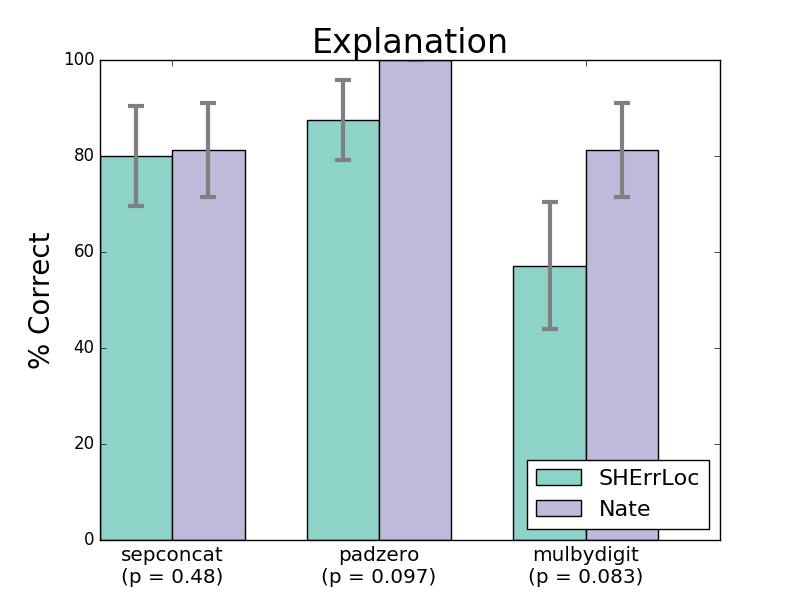
\includegraphics[width=0.7\linewidth]{nate/user-study-reason.png}
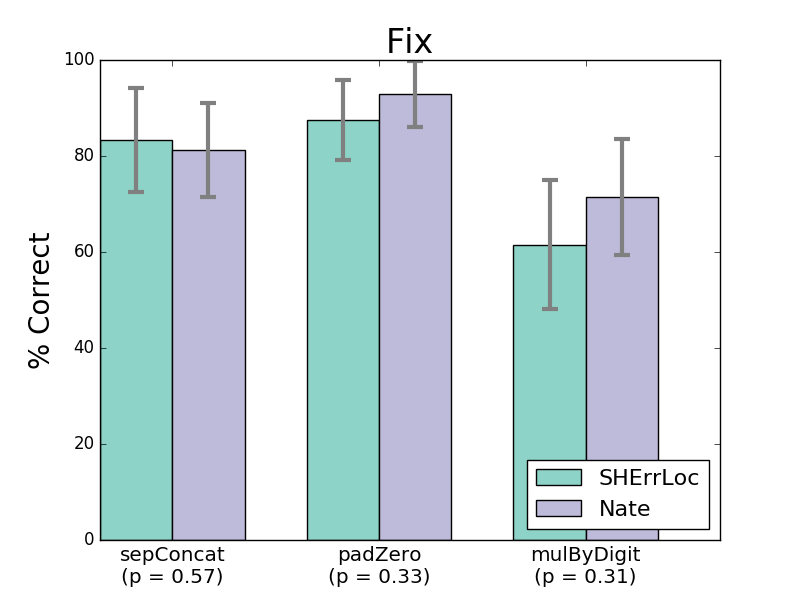
\includegraphics[width=0.7\linewidth]{nate/user-study-fix.png}
% \end{minipage}
% }
% \vspace{3ex}
\caption{A classification of students' explanations and fixes for type
  errors, given either \sherrloc or \toolname's blame assignment.
  %
  The students given \toolname's location generally scored
  better than those given \sherrloc's.
  %
  We report the result of a one-sided Mann-Whitney $U$ test for
  statistical significance in parentheses.}
\label{fig:results-user-study}
\end{figure}

\paragraph{Results}
%
The measured kappa values were $\kappa = 0.68$ for the explanations and
$\kappa = 0.77$ for the fixes; while there is no formal notion for what
consititutes strong agreement~\cite{Krippendorff2012-wd}, kappa values
above $0.60$ are often called ``substantial''
agreement~\cite{Landis1977-ey}.
%
Figure~\ref{fig:results-user-study} summarizes a single annotator's
results, which show that students given \toolname's blame assignment
were generally more likely to correctly explain and fix the type error
than those given \sherrloc's.
%
While there was no discernible difference between \toolname and
\sherrloc for |sepConcat|, \toolname responses for |padZero| and
|mulByDigit| were marked correct 5--30\% more often than the \sherrloc
responses.
%
The results appear to show a trend in favor of \toolname;
%
however, they are not statistically significant so
we cannot discount the possibility of confounding factors.
%


%%% Local Variables:
%%% mode: latex
%%% TeX-master: "main"
%%% End:

%\mysubsection{Qualitative Evaluation}
\mysubsection{Interpreting Specific Predictions}
\label{sec:nate:qualitative}

Next, we present a \emph{qualitative} evaluation
that compares the predictions made by our classifiers
with those of \sherrloc.
%
In particular, we demonstrate, with a series of example programs from
our student dataset, how our classifiers are able to use past student
mistakes to make more accurate predictions of future fixes.
%
We also take this opportunity to examine some of the specific features
our classifiers use to assign blame.
%
For each example, we provide
%
(1) the code;
%
(2) \hlSherrloc{\sherrloc's} prediction;
%
(3) our \hlTree{\dectree's} prediction; and
%
(4) an \emph{explanation} of why our classifier made its prediction, in
terms of the features used and their values.
%
We choose the \dectree classifier for this section as its model is more
easily interpreted than the MLP.\@
%
We also exclude the \ExprSize feature from the model used in this
section, as it makes the predictions harder to motivate, and as we saw
in \autoref{sec:nate:feature-utility} it does not appear to contribute
significantly to the model's accuracy.

We explain the predictions by analyzing the paths induced in
the decision tree by the features of the input expressions.
%
Recall that each node in a decision tree contains a simple predicate of
the features, \eg ``is feature $v_j$ enabled?'', which determines
whether a sample will continue down the left or right subtree.
%
Thus, we can examine the predicates used and the values of the
corresponding features to explain \emph{why} our \dectree made its
prediction.
%
We will focus particularly on the enabled features, as they generally
provide more information than the disabled features.
%
Furthermore, each node is additionally labeled with the ratio of
``blamed'' vs ``not-blamed'' training expressions that passed through
it.
%
We can use this information to identify particularly important
decisions, \ie we consider a decision that changes the ratio to be more
interesting than a decision that does not.

%
% We will also attempt, for each program, to explain \emph{why} the
% Decision Tree made its prediction, by analyzing the paths induced
% by the programs.

\mysubsubsection{Failed Predictions}
\label{sec:nate:failed-predictions}

We begin with a few programs where our classifier fails to
make the correct prediction.
%
For these programs we will additionally \hlFix{highlight} the
correct blame location.

\mypara{Constructing a List of Duplicates}
% data/sp14/0219.ml
Our first program is a simple recursive function |clone| that takes an
item |x| and a count |n|, and produces a list containing |n| copies of
|x|.
%
% \begin{ecode}
%   let rec clone x n =
%     let loop acc n =
%       if n <= 0 then
%         acc
%       else
%         (*@\colorbox{red!50}{clone}@*) ==([==_=x=_==] @ acc)== (n - 1) in
%     loop [] n
% \end{ecode}
\begin{ecode}
  let rec clone x n =
    let loop acc n =
      if n <= 0 then
        acc
      else
        (*@\hlFix{clone} \hlSherrloc{([\hlTree{x}] @\ acc)}@*) (n - 1) in
    loop [] n
\end{ecode}
% \ES{TODO: our 2nd prediction matches \sherrloc and \ocaml (occurs check), correct fix is to replace recursive call to clone with loop}
%
The student has defined a helper function |loop| with an accumulator
|acc|, likely meant to call itself tail-recursively.
%
Unfortunately, she has called the top-level function |clone| rather than
|loop| in the |else| branch, this induces a cyclic constraint |'a = 'a list|
for the |x| argument to |clone|.

Our classifier incorrectly predicts that the use of |x| in the recursive
call is the most likely source of the error.
%
Our second prediction coincides with \sherrloc (and \ocaml), blaming the
the first argument to |clone|.
%
This is also incorrect, but may be more helpful than our first
prediction --- if our student decides that she has certainly provided
the correct \emph{argument}, an alternative explanation is that
perhaps she has called the wrong \emph{function}.

We confess that both of these predictions are difficult to explain by
examining the induced paths.
%
In particular, both predictions only reference the expression's context,
which is surprising.
%
Much clearer is why we fail to blame the occurrence of |clone|, the two
enabled features on the path are:
%
(1) the parent is an application; and
%
(2) |clone| has a function type.
%
The model seems to have learned that programmers typically call the
correct function.

\mypara{Currying Considered Harmful?}
% data/sp14/1204.ml
Our next example is another ill-fated attempt at |clone|.
%
\begin{ecode}
  let rec clone x n =
    let rec loop (*@\hlFix{x n acc}@*) =
      if n < 0 then
        acc
      else
        (*@\hlSherrloc{loop} \hlTree{(x, (n - 1), (x :: acc))}@*) in
    loop (x, n, [])
\end{ecode}
%
The issue here is that \ocaml functions are \emph{curried} by default
--- \ie they take their arguments one at a time --- but our student has
called the inner |loop| with all three arguments in a tuple.
%
Many experienced functional programmers would choose to keep |loop|
curried and rewrite the calls, however our student decides instead to
\emph{uncurry} |loop|, making it take a tuple of arguments.
%
\sherrloc blames the recursive call to |loop| while our classifier
blames the tuple of arguments --- a reasonable suggestion, but not
the answer the student expected.

We fail to blame the definition of |loop| because it is defining a
function.
%
First, note that we represent |let f x y = e|\ \ as\ \ |let f = fun x -> fun y -> e|,
thus a change to the pattern |x| would be treated as a change to the outer
|fun| expression.
%
With this in mind, we can explain our failure to blame the definition of
|loop| (the outer |fun|) as follows:
%
(1) it has a function type;
%
(2) its child is a |fun|; and
%
(3) its parent is a |let|.
%
Thus it appears to the model that the outer |fun| is simply part of a
function definition, a common and innocuous phenomenon.

% \mypara{Composing Functions}
% % data/sp14/3041.ml
% Next, let us consider the |pipe| function that composes a list of
% functions, \ie given a list of functions |[f;g;h]|, |pipe| produces the
% function |fun x -> h (g (f x))|.
% %
% \begin{ecode}
%   let pipe fs =
%     let f a x y = ==y== __(a y)__ in
%     let base x = x in
%     List.fold_left f base fs
% \end{ecode}
% %
% The error in our student's code is that she has applied |y| rather than
% |x| to the result of |a y|.
% %
% \sherrloc correctly blames the first occurrence of |y|, while our
% classifier (incorrectly) blames the application |a y| (\ocaml blames
% the occurrence of |base| on line 4).
% %
% \ES{this has the same explanation as the 1st clone above}

\mysubsubsection{Correct Predictions}
\label{sec:nate:correct-predictions}

Next, we present a few indicative programs where our first prediction is
correct, and all of the other tools' top three predictions are
incorrect.

\mypara{Extracting the Digits of an Integer}
% data/sp14/2176.ml
Consider first a simple recursive function |digitsOfInt| that extracts
the digits of an |int|.
%
\begin{ecode}
  let rec digitsOfInt n =
    if n <= 0 then
      []
    else
      [n mod 10] @ (*@\hlTree{[ \hlSherrloc{digitsOfInt (n / 10)} ]}@*)
\end{ecode}
%
Unfortunately, the student has decided to wrap the recursive call to
|digitsOfInt| with a list literal, even though |digitsOfInt| already
returns an |int list|.
%
Thus, the list literal is inferred to have type |int list list|, which
is incompatible with the |int list| on the left of the |@| (list append)
operator.
%
Both \sherrloc and the \ocaml compiler blame the recursive call for
returning a |int list| rather than |int|, but the recursive call is
correct!

As our \dectree correctly points out (with high confidence), the fault
lies with the list literal \emph{surrounding} the recursive call, remove
it and the type error disappears.
%
An examination of the path induced by the list literal reveals that our
\dectree is basing its decision on the fact that
%
(1) the expression is a list literal;
%
(2) the child expression is an application, whose return type mentions |int|; and
%
(3) the parent expression's type mentions |list|.
%
Interestingly, \dectree incorrectly predicts that the child application
should change as well, but it is less confident of this prediction and
ranks it below the correct blame assignment.

\mypara{Padding a list}
% data/sp14/0442.ml
Our next program, |padZero|, is given two |int list|s as input, and must
left-pad the shorter one with enough zeros that the two output lists
have equal length.
%
The student first defines a helper |clone|.
%
\begin{ecode}
  let rec clone x n =
    if n <= 0 then
      []
    else
      x :: clone x (n - 1)
\end{ecode}
%
Then she defines |padZero| with a branch to determine which
list is shorter, followed by a |clone| to zero-pad it.
%
\lstset{firstnumber=last}
\begin{ecode}
  let padZero l1 l2 =
    let n = List.length l1 - List.length l2 in
    if n < 0 then
      (clone 0 ((-1) * n) @ l2, l2)
    else
      (l1, (*@\hlTree{\hlSherrloc{clone 0 n} :: l2}@*))
\end{ecode}
\lstset{firstnumber=1}
%
Alas, our student has accidentally used the |::| operator rather than
the |@| operator in the |else| branch.
%
\sherrloc and \ocaml correctly determine that she cannot cons the
|int list| returned by |clone| onto |l2|, which is another |int list|,
but they decide to blame the call to |clone|, while our
\dectree correctly blames the |::| constructor.

Examining the path induced by the |::|, we can see that our
\dectree is influenced by the fact that:
%
(1) |::| is a constructor; %the expression is a constructor (not specifically |::|);
%
(2) the parent is a tuple; and
%
(3) the leftmost child is an application.
%
We note that first fact appears to be particularly significant; an
examination of the training samples that reach that decision
reveals that, before observing the \textsc{Is-Constructor} feature the
classifier is slightly in favor of predicting ``blame'', but afterwards
it is heavily in favor of predicting ``blame''.
%
Many of the following decisions change the balance back towards ``no
blame'' if the ``true'' path is taken, but the |::| constructor always
takes the ``false'' path.
%
It would appear that our \dectree has learned that constructors are
particularly suspicious, and is looking for exceptions to this general
rule.
%
% \ES{FIXME: this is probably super confusing, checking with Huma to see
%   if we can get a nice graph to illustrate what's happening..}

Our \dectree correctly predicts that the recursive call blamed by
\sherrloc should not be blamed; a similar examination suggests that the
crucial observation is that the recursive call's parent is a data
constructor application.
%



% ES: decision tree gets this one wrong, may want to find something else
% \begin{ecode}
%   let rec sepConcat sep sl =
%     match sl with
%     | [] -> ""
%     | h::t ->
%         let f a x = a ^ (sep ^ x) in
%         List.fold_left f h t

%   let stringOfList f l = sepConcat "; " __[ "["; ___=List.map f l=___; "]" ]__
% \end{ecode}

% \ES{I don't much like this example anymore..}
% \mypara{Computing the Fixed Point of a Function}
% % data/sp14/1266.ml
% Finally, our students must write a |fixpoint| function that computes the
% fixed point of a given function |f|, starting from an initial value |b|.
% %
% As a hint, we first have them write a |wwhile| function that performs the
% functional equivalent of a \texttt{while}-loop, repeatedly passing a function's
% output back in until it receives a (boolean) signal to stop.
% %
% \begin{ecode}
%   let rec wwhile (f, b) =
%     match f b with
%     | (x, false) -> x
%     | (x, true)  -> wwhile (f, x)
% \end{ecode}
% \lstset{firstnumber=last}
% %
% The |fixpoint| function can then be written as a clever instantiation of
% the arguments to |wwhile|.
% %
% \begin{ecode}
%   let fixpoint (f, b) =
%     let g = __let bb = f b in ___=(bb, (bb = b))=_ in
%     wwhile (g, b)
% \end{ecode}
% \lstset{firstnumber=1}
% %
% Sadly, our student has forgotten that |g| should itself be a function.
% %
% As a result, she passes a pair of a \emph{pair} and a starting value to
% |wwhile|, rather than a pair of a \emph{function} and a starting value.
% %
% \sherrloc deduces that the call to |wwhile| is likely correct (\ocaml
% actually blames the use of |g|), but identifies the construction of the
% pair inside |g| as the most likely culprit, while our \dectree correctly
% identifies the \emph{definition} of |g| as the source of the error.
% %
% Our \dectree appears to base its prediction, with complete confidence,
% on the fact that:
% %
% (1) the parent expression is a |let|;
% %
% (2) the right child is a tuple; and finally
% %
% (3) the current expression is a |let|.
% %



%%% Local Variables:
%%% mode: latex
%%% TeX-master: "main"
%%% End:

\mysubsection{Threats to Validity}
\label{sec:nate:validity}

Although our experiments demonstrate that our technique can pinpoint type
errors more accurately than the state of the art and that our features are
relevant to blame assignment, our results may not generalize.

One threat to validity associated with supervised machine learning is
overfitting (\ie learning a model that is too complex with respect to
the data).
%
A similar issue that arises in machine learning is model stability (\ie
can small changes to the training set produce large changes in the model?).
%
We mitigate these threats by:
%
(1) using separate training and testing datasets drawn from distinct
student populations (\autoref{sec:nate:quantitative}), demonstrating the
generality of our models; and
%
(2) via cross-validation on the joint dataset
(\autoref{sec:nate:feature-utility}), which demonstrates the stability of our
models by averaging the accuracy of 10 models trained on distinct
subsets of the data.

Our benchmarks were drawn from students in an undergraduate course and
may not be representative of other student populations.
%
We mitigate this threat by including the largest empirical evaluation of
type error localization that we are aware of: over 4,500 pairs of
ill-typed programs and fixes from two instances of the course, with
programs from 102 different students.
%
We acknowledge, of course, that students are not industrial programmers
and our results may not translate to large-scale software development;
however, we are particularly interested in aiding novice programmers
as they learn to work inside the type system.

A related threat to construct validity is our definition of the immedate
next well-typed program as the intended ground truth answer (see
\autoref{sec:nate:overview}, Challenge 2). Students may, in theory, submit
intermediate well-typed program ``rewrites'' between the original ill-typed
program and the final intended answer. Our approach to discarding outliers
(see \autoref{sec:nate:evaluation}) is designed to mitigate this threat.

Our removal of program pairs that changed too much, where our oracle
could not identify the blame of the other tools, or where the other
tools timed out or encountered unsupported language features is another
threat to validity.
%
It is possible that including the programs that changed excessively
would hurt our models, or that the other tools would perform
better on the programs with unsupported language features.
%
We note however that
%
(1) outlier removal is a standard technique in machine learning%
%\ES{CITE?}
; and
%
(2) our Top-1 accuracy margin is large enough that even if we assumed
that \sherrloc were perfect on all excluded programs,
% it would only tie our \hiddenFH. % in Top-1 accuracy.
we would still lead by 10 points.
%
%\ES{I think this is accurate, but should double check..}

Examining programs written in \ocaml as opposed to \haskell or any other
typed functional language poses yet another threat, common type errors
may differ in different languages.
%
\ocaml is, however, a standard target for research in type error
localization and thus our choice admits a direct comparison with prior
work.
%
Furthermore, the functional core of \ocaml that we support does not
differ significantly from the functional core of \haskell or SML, all of
which are effectively lambda calculi with a Hindley-Milner-style type
system.
% \footnote{\haskell's type classes are a notable exception, they
%   are also known to cause confusing type errors and would be interesting
%   to study as well.}

Finally, our use of student fixes as oracles
% for the source of type errors
assumes that students are able to correctly identify
the source of an error.
%
As the students are in the process of learning the language and type
system, this assumption may be faulty.
%
It may be that \emph{expert} users would disagree with many of the
student fixes, and that it is harder to learn a model of expert fixes,
or that the state of the art would be better at predicting expert fixes.
%
As we have noted before, we believe it is reasonable to use student
fixes as oracles because the student is the best judge of what she
\emph{intended}.

\mysection{Limitations}
\label{sec:nate:discussion}

We have shown that we can outperform the state of the art in type error
localization by learning a model of the errors that programmers make,
using a set of features that closely resemble the information the type
checker sees.
%
% However, there is certainly room for improvement.
%
In this section we highlight some limitations of our approach and
potential avenues for future work.

% \mysubsection{Limitations}
% \label{sec:nate:limitations}

\paragraph{User-Defined Types}
Probably the single biggest limitation of our technique is that we have
(a finite set of) features for specific data and type constructors.
%
Anything our models learn about errors made with the |::| constructor or
the |list| type cannot easily be translated to new, user-defined
datatypes the model has never encountered.
%
We can mitigate this, to some extent, by adding generic
syntactic features for data constructors and match expressions, but it
remains to be seen how much these help. % \ES{TODO: UW data!}.
%
Furthermore, there is no obvious analog for transferring knowledge to
new type constructors, which we have seen are both more compact and
helpful.

As an alternative to encoding information about \emph{specific}
constructors, we might use a more abstract representation.
%
For example, instead of modeling |x :: 2| as a |::| constructor with a
right child of type |int|, we might model it as some (unknown) constructor
whose right child has an incompatible type.
%
We might symmetrically model the |2| as an integer literal whose type is
incompatible with its parent.
%
Anything we learn about |::| and |2| can now be transferred directly to
yet unseen types, but we run the risk generalizing \emph{too much} ---
\ie perhaps programmers make different mistakes with |list|s than they
do with other types, and are thus likely to choose different fixes.
%
Balancing the trade-off between specificity and generalizability appears
to be a challenging task.

% \begin{itemize}
% \item Hard to support in general, as each data and type constructor gets
%   its own set of syntactic features.
% \item Attempt to mitigate by adding generic ``is-datacon'' and
%   ``is-match'' feature, unclear how much it will help
% \end{itemize}

\paragraph{Additional Features}
There are a number of other features that could improve the model's
ability to localize errors, that would be easier to add than
user-defined types.
%
For example, each occurrence of a variable knows only its type and its
immediate neighbors, but it may be helpful to know
about \emph{other} occurrences of the same variable.
%
If a variable is generally used as a |float| but has a
single use as an |int|, it seems likely that the
latter occurrence (or context) is to blame.
%
Similarly, arguments to a function application are not aware of the
constraints imposed on them by the function (and vice versa),
they only know that they are occurring in the context of an application.
%and the type of the application itself.
%
Finally, \emph{n-grams} on the token stream have proven effective for
probabilistic modeling of programming languages
\citep{Hindle2012-hf,Gabel2010-el}, we may find that they aid in
our task as well.
%
For example, if the observed tokens in an expression diverge from the
n-gram model's predictions, that indicates that there is something
unusual about the program at that point, and it may signal an error.

% \begin{itemize}
% \item def-use chains
% \item connect function and arguments in application (right now each only know about the application itself)
% \item ??
% \end{itemize}

\paragraph{Independent vs Joint Predictions}
We treat each sub-expression as if it exists in a vacuum, but in reality
the program has a rich \emph{graphical} structure, particularly if one adds
edges connecting different occurrences of the same variable.
%
\citet{Raychev2015-jg} have used these richer models to great effect to
make \emph{interdependent} predictions about programs, \eg
de-obfuscating variable names or even inferring types.
%
One could even view our task of locating the source of an error as simply
another property to be predicted over a graphical model of the program.
%
One of the key advantages of a graphical model is that the predictions
made for one node can influence the predictions made for another node,
this is known as \emph{structured learning}.
%
For example, if, given the expression |1 + true|, we predict |true| to
be erroneous, we may be much less likely to predict |+| as erroneous.
%
We compensate somewhat for our lack of structure by adding contextual
features and by ranking our predictions by ``confidence'', but it would
be interesting to see how structured learning over graphical models
would perform.


%%% Local Variables:
%%% mode: latex
%%% TeX-master: "main"
%%% End:

\mysection{Related Work}
\label{sec:nate:related-work}
\label{sec:nate:type-error-diagnosis}

In this section we describe two relevant aspects of related work:
%
programming languages approaches to diagnosing type errors, and
%
software engineering approaches to fault localization.
%
% applying machine learning techniques to problems in programming languages.
%
% \mysubsection{Type Error Diagnosis}
%% Languages with static type systems and type inference produce type
%% errors that novices often perceive as difficult to
%% interpret~\citep{Wand1986-nw}.
%% %
%% For example, approaches based on Hindley-Milner or other constraint
%% systems typically have the issue that when the constraint $\alpha=\beta$
%% is violated, the system cannot know whether the user should intend to
%% fix $\alpha$ or $\beta$ and must thus report the discrepancy in a
%% generic manner.
%% %
%% As a result, a number of approaches have been proposed to
%% more precisely localize the type error,
%% give clearer error messages, or
%% fix the error automatically.
%
% The technique most related to our work is \ES{TODO}.  It has been shown
% to be quite good at \ES{TODO}. However, we choose to focus on \ES{TODO},
% and our approach contains \ES{TODO}, which is not present in previous
% work.

\paragraph{Localizing Type Errors}
It is well-known that the original Damas-Milner
algorithm $\mathcal{W}$ produces errors far
from their source, that novices percieve as
difficult to interpret~\citep{Wand1986-nw}.
%
%% The type checker collects typing constraints as it traverses the
%% program, and it crucially assumes that if a constraint can be safely
%% added to the set of assumptions (\ie no type error has been found yet),
%% then the constraint can be \emph{assumed} to be correct.
%
The type checker reports an error the moment
it finds a constraint that contradicts one
of the assumptions, blaming the new inconsistent
constraint, and thus it is extremely sensitive
to the order in which it traverses the source
program (the infamous ``left-to-right''
bias~\citep{McAdam1998-ub}).
%
Several alternative traversal have been proposed,
\eg top-down rather than bottom-up~\citep{Lee1998-ys},
or a \emph{symmetric} traversal that checks
sub-expressions independently and only reports an
error when two inconsistent sets of constraints are
merged~\citep{McAdam1998-ub,Yang1999-yr}.
%
%\paragraph{Slicing}
Type error \emph{slicing}~\citep{Haack2003-vc,Tip2001-qp,Rahli2010-ps}
overcomes the constraint-order bias by extracting a
complete and minimal subset
of terms that contribute to the error, \ie all of the
terms that are required for it to manifest and no more.
%
Slicing typically requires rewriting the type checker with a
specialized constraint language and solver, though
\citet{Schilling2011-yf} shows how to turn any type checker into a
slicer by treating it as a black-box.
%
While slicing techniques guarantee enough information to diagnose the
error, they can fall into the trap of providing \emph{too much}
information, producing a slice that is not much smaller than
the input. %original. % input program.

\paragraph{Finding Likely Errors}
Thus, recent work has focused on finding the \emph{most likely} source
of a type error.
%
\citet{Zhang2014-lv} use Bayesian reasoning to search the constraint
graph for constraints that participate in many unsatisfiable paths and
relatively few satisfiable paths, based on the intuition that the
program should be mostly correct.
%
\citet{Pavlinovic2014-mr} translate the localization problem into a
MaxSMT problem, asking an off-the-shelf solver to find the smallest
set of constraints that can be removed such that the resulting system is
satisfiable.
%
\citet{Loncaric2016-uk} improve the scalability of
\citeauthor{Pavlinovic2014-mr} by reusing the existing type checker as
a theory solver in the Nelson-Oppen~\citeyear{Nelson1979-td}
style, and thus require only a MaxSAT solver.
%
All three of these techniques support \emph{weighted} constraints to
incorporate knowledge about the frequency of different errors,
but only \citeauthor{Pavlinovic2014-mr} use the weights, setting them to
the size of the term that induced the constraint.
%
In contrast, our classifiers learn a set of heuristics for predicting
the source of type errors by observing a set of ill-typed programs and
their subsequent fixes, in a sense using \emph{only} the weights and no
constraint solver.
%
It may be profitable to combine both approaches, \ie learn a set of good
weights for one of the above techniques from our training data.

\paragraph{Explaining Type Errors}
In this paper we have focused solely on the task of \emph{localizing} a
type error, but a good error report should also \emph{explain} the
error.
%
\citet{Wand1986-nw}, \citet{Beaven1993-hb}, and \citet{Duggan1996-by}
attempt to explain type errors by collecting the chain of inferences
made by the type checker %--- essentially the typing derivation ---
and presenting them to the user.
%
% Such explanations can be lengthy, as an attempt to compress the
% explanation \citet{Yang2000-kz} presents a visualization of the
% inference process.
%
\citet{Gast2004-zd} produces a slice enhanced by arrows
showing the dataflow from sources with different types to a
shared sink, borrowing the insight of dataflows-as-explanations from
\textsc{MrSpidey}~\citep{Flanagan1996-bu}.
%
\citet{Hage2006-hc} catalog a set of heuristics for
improving the quality of error messages by examining errors made by
novices.
%
\citet{Heeren2003-db}, \citet{Christiansen2014-qc}, and
\citet{Serrano2016-oo} extend the ability to customize error messages to
library authors, enabling \emph{domain-specific} errors.
%
%\paragraph{Interactive Explanations}
Such \emph{static} explanations of type errors run the risk of
overwhelming the user with too much information, it may be preferable to
treat type error diagnosis as an \emph{interactive} debugging session.
%
\citet{Bernstein1995-yj} extend the type inference procedure to handle
\emph{open} expressions (\ie with unbound variables), allowing users to
interactively query the type checker for the types of sub-expressions.
%
\citet{Chitil2001-td} proposes \emph{algorithmic debugging} of type
errors, presenting the user with a sequence of yes-or-no questions about
the inferred types of sub-expressions that guide the user to a specific
explanation.
%
\citet{Seidel2016-ul} explain type errors by searching for inputs that
expose the \emph{run-time} error that the type system prevented, and
present users with an interactive visualization of the erroneous
computation.

%% RJ-CUT-ME \paragraph{Programmatic Explanations}
%% RJ-CUT-ME %
%% RJ-CUT-ME The best explanation of a type error, however, might be given by an
%% RJ-CUT-ME expert, \eg the compiler or library author.
%% RJ-CUT-ME %
%% RJ-CUT-ME \citet{Hage2006-hc} catalog a set of heuristics for
%% RJ-CUT-ME improving the quality of error messages by examining errors made by
%% RJ-CUT-ME novices.
%% RJ-CUT-ME %
%% RJ-CUT-ME \citet{Heeren2003-db}, \citet{Christiansen2014-qc}, and
%% RJ-CUT-ME \citet{Serrano2016-oo} extend the ability to customize error messages to
%% RJ-CUT-ME library authors, enabling \emph{domain-specific} errors.
%
% The 8.0 release of the
% Glasgow Haskell Compiler\footnote{\url{https://ghc.haskell.org/trac/ghc/wiki/Proposal/CustomTypeErrors}}
% incorporates these ideas, allowing library authors to supply
% custom errors when type-class resolution or type-family reduction fail,
% but not for ordinary unification failures.


\paragraph{Fixing Type Errors}
Some techniques go beyond explaining or locating a type error,
and actually attempt to \emph{fix} the error automatically.
%
\citet{Lerner2007-dt} searches for fixes by enumerating a
set of local mutations to the program and querying the type checker to
see if the error remains.
%
\citet{Chen2014-gd} use a notion of \emph{variation-based} typing to
track choices made by the type checker and enumerate potential
% type (and expression)
changes that would fix the error.
%
They also extend the algorithmic debugging technique of
\citeauthor{Chitil2001-td} by allowing the user to enter the expected
type of specific sub-expressions and suggesting fixes based on these
desired types \citeyear{Chen2014-vm}.
%
Our classifiers do not attempt to suggest fixes to type errors, but it
may be possible to do so by training a classifier to predict the
syntactic class of each expression in the \emph{fixed} program --- we
believe this is an exciting direction for future work.

\paragraph{Fault Localization}
%
Given a defect, \emph{fault localization} is the task of identifying
``suspicious'' program elements (\eg lines, statements) that are likely
implicated in the defect %(\ie that should be changed to fix the defect)
%
--- thus, type error localization can be viewed as an instance of fault
localization.
%
The best-known fault localization technique is likely Tarantula, which
uses a simple mathematical formula based on measured information from
dynamic normal and buggy runs~\citep{Jones2002-us}.
%
Other similar approaches, including those of \citet{Chen2002-qz} and
\citet{Abreu2006-fn,Abreu2007-mu} consider alternate features of
information or refined formulae and generally obtain more precise
results; see \citet{Wong2009-pd} for a survey.
%
While some researchers have approached such fault localization with an
eye toward optimality (\eg \citet{Yoo2013-rw} determine optimal
coefficients), in general such fault localization approaches are limited
by their reliance on either running tests or including relevant
features.
%
For example, Tarantula-based techniques require a normal and a buggy run
of the program.
%
By contrast, we consider incomplete programs with type errors that may
not be executed in any standard sense.
%
Similarly, the features available influence the classes of defects that
can be localized.
%
For example, a fault localization scheme based purely on control flow features
will have difficulty with cross-site scripting or SQL code injection
attacks, which follow the same control flow path on normal and buggy
runs (differing only in the user-supplied data).
%
Our feature set is comprised entirely of syntactic and typing features,
a natural choice for type errors, but it would likely not
generalize to other defects.


% \subsection{Machine Learning for Programming Languages}
% \label{sec:nate:ml-pl}



%%% Local Variables:
%%% mode: latex
%%% TeX-master: "main"
%%% End:

\mysection{Conclusion}
\label{sec:nate:conclusion}

We have presented \toolname, which
combines modern statistical methods
with domain-specific feature engineering
to open the door to a new data-driven
path towards precise error localization,
significantly outperforming the
state of the art on a new benchmark
suite comprising 5,000 student programs.
%
%%% RJNUKEDME   \toolname
%%% RJNUKEDME   translates pairs of
%%% RJNUKEDME   blame-labeled ill-typed
%%% RJNUKEDME   programs into bags-of-abstracted-terms,
%%% RJNUKEDME   and then trains a classifier
%%% RJNUKEDME   to predict whether a feature vector
%%% RJNUKEDME   should get a blame label.
%%% RJNUKEDME   % that
%%% RJNUKEDME   % predicts the value of the
%%% RJNUKEDME   % whether a feature vector gets
%%% RJNUKEDME   % a blame label.
%%% RJNUKEDME   %
%%% RJNUKEDME   Given a new ill-typed program,
%%% RJNUKEDME   we extract its bag-of-abstracted-terms
%%% RJNUKEDME   to compute the blame label for each
%%% RJNUKEDME   term and rank the predictions based
%%% RJNUKEDME   on the model's confidence, to select
%%% RJNUKEDME   the top 1--3 blame assignments to
%%% RJNUKEDME   present to the user.
%%% RJNUKEDME
%%% RJNUKEDME   We have evaluated our approach with
%%% RJNUKEDME   five different classifiers on a suite
%%% RJNUKEDME   of over 4,500 student programs.
%
We found that while machine learning
over syntactic features of each term in isolation
performs worse than existing
purely constraint-based approaches, % (\eg \ocaml, \sherrloc),
augmenting the data with a single feature corresponding to
the type error slice brings our
classifiers up to par with the state of the art,
and further augmenting the data with
features of an expression's parent and children
allows our classifiers to outperform
the state of the art by \ToolnameWinSherrloc
percentage points.

% We find that while machine
% learning on its own performs slightly worse
% than existing purely constraint based
% approaches (\eg \ocaml, \sherrloc), once
% we augment the data with feature abstraction
% corresponding to the \emph{type error slice}~\cite{Tip2001-qp},
% the resulting models models outperform
% the state of the art by up to 18
% percentage points.


As with other forms of machine learning,
a key concern is that of \emph{data-set bias}: are
\toolname's models specific
to our data set, would they fail on
\emph{other} programs?
%
We address this concern in two ways.
%
First, we partition the data by year,
and show that models learned from one
year generalize to, \ie perform nearly
as well on, the programs from the other
year.
%
Second, we argue that in our setting
this bias is a \emph{feature} (and not
a bug): it allows \toolname to \emph{adapt}
to the kinds of errors that programmers
(specifically novices, who are in greatest
need of precise feedback) actually make,
rather than hardwiring the biases of
experts who % , by dint of their
% training and experience,
may suffer from blind spots. % with regards to such problems.
%
In this regard, we are particularly pleased
that our classifiers can be trained on a
modest amount of data, \ie a single course's
worth, and envision a future where each course
comes equipped with a model of its students' errors.



%%% Local Variables:
%%% mode: latex
%%% TeX-master: "main"
%%% End:


%\part{Conclusion}
\chapter{Conclusion}

\appendix
\chapter{Proofs}
\chapter{Proofs for Section~\ref{sec:nanomaly:searching-witness}}
\label{sec:nanomaly:proofs}

% \begin{proof}[Proof of Lemma~\ref{lem:force-inst}]
%   By case analysis on the evaluation rules.
%   %
%   If $\ptype{\trace}{f} \neq \ptype{\trace'}{f}$ then,
%   % one of the holes in $f$'s
%   % argument must have been instantiated with a concrete value at the last step.
%   by the definition of $\ptype{\trace}{f}$, $\tsu \neq \tsu'$, as \thole
%   does not change.
%   %
%   % An examination of the rules shows that only place this happens is
%   % in the second case of \forcesym.
%   An examination of the rules shows that only \forcesym can update \tsu.


%   Furthermore, an examination of \forcesym immediately shows that in the
%   cases where \forcesym returns \stuck, \tsu\ is unmodified. Thus only
%   \emph{successful} calls to \forcesym can change \tsu\ and, by
%   extension, \ptype{\trace}{f}.

%   % - narrow(leaf[t_1], t_2, \sigma, \theta)
%   %   - t_1 != \alpha because E-Leaf always creates fresh \alpha
%   %   - what aboue t_2? could mention \alpha in E-Node-*..

%   % By case analysis on the evaluation rules. As above we are only
%   % concerned with the sucessful steps, and can thus ignore the
%   % \rulename{E-*-Bad} rules.

%   % In each case we will show that only
%   % the calls to \forcesym can change the partial input type of $f$.

%   % \begin{description}
%   % % \item[Case \reholegood] \hastype{\ehole}{\thole}, which is
%   % %   alpha-equivalent to \typeof{\vhole{\thole}}, thus this step does not
%   % %   change the partial type.
%   % \item[Case \replusgood] Since narrowing succeeded on $v_1$ and $v_2$,
%   %   they must have both either been ints or unconstrained holes.
%   %   The only way the partial input type could have changed is if one or the
%   %   other was a hole, and was instantiated by \forcesym.
%   % \item[Case \rulename{E-If-Good-\{1,2\}}] Since narrowing succeeded on
%   %   $v$, it must have either been a bool or an unconstrained hole.
%   %   The only way the partial input type could have changed is if $v$ was a
%   %   hole and was instantiated by \forcesym.
%   % \item[Case \reappgood] Since narrowing succeeded on $v$, it must have
%   %   either been a lambda or an unconstrained hole. The only way the
%   %   partial input type could have changed is if $v$ was a hole and was
%   %   instantiated by \forcesym.
%   % \item[Case \releafgood] This rule does not call \forcesym, thus it
%   %   cannot change the partial input type, and cannot have been applied.
%   % \item[Case \renodegood] In this case the partial input type could have
%   %   changed if any of $v_1$, $v_2$, or $v_3$ were unconstrained holes.
%   %   Since both \forcesym calls succeeded \emph{and} the partial input
%   %   type changed

%   %   Since narrowing succeeded on $v_2$ and $v_3$,
%   %   they must have both been trees or unconstrained holes

%   %   \ES{come back to this, not entirely clear it
%   %     holds as we might learn the element type from one of the subtrees}
%   % \item[Case \rulename{E-Case-Good\{1,2\}}] Since narrowing succeeded on
%   %   $v$, it must have either been a tree or an unconstrained hole.
%   %   The only way the partial input type could have changed is if $v$ was a
%   %   hole and was instantiated by \forcesym.
%   % \end{description}
% \end{proof}


% \begin{proof}[Proof of Lemma~\ref{lem:refine-partial}]
%   By case analysis on the evaluation rules.

%   We can immediately discharge the $\rulename{E-*-Bad}$ rules as they
%   result in the \stuck state, and by Lemma~\ref{lem:force-inst} we know
%   that these rules cannot change \ptype{\trace}{f} at all.

%   % and
%   % an inspection of \forcesym shows that when \forcesym returns \stuck,
%   % it does not modify \vsu or \tsu. Furthermore, \forcesym is the only
%   % procedure that can modify the substitutions.

%   % For the remainder of the rules we must
%   % consider how they might affect both the input (by instantiating holes)
%   % and output components of the partial type.

%   % We will call a type hole \thole \emph{unconstrained} if applying the
%   % current type substitution \subst{\tsu}{\thole} produces a type hole.

%   \begin{description}
%   \item[Case \replusgood] Both $v_1$ and $v_2$ successfully narrowed to
%     \tint, so they must have either been ints or unconstrained
%     holes. Thus partial input type compatibility is preserved.

%     % \hastype{\eplus{v_1}{v_2}}{\thole} and
%     % \hastype{n}{\tint}, so partial type compatibility of the output is
%     % preserved.
%   \item[Case \rulename{E-If-Good-\{1,2\}}] $v$ successfully narrowed to
%     \tbool, so it must have either been a bool or an unconstrained hole.
%     Thus partial input type compatibility is preserved.

%     % \hastype{\eif{v}{e_1}{e_2}}{\thole}, which is compatible with any
%     % type $e_1$ or $e_2$ might have, so partial type compatibility of the
%     % output is also preserved.
%   \item[Case \reappgood] $v_1$ successfully narrowed to \tfun, so it
%     must have either been a lambda or an unconstrained hole, so partial
%     input type compatibility is preserved.

%     % \hastype{\eapp{v_1}{v_2}}{\thole}, which is compatible with any type
%     % $e$ might have, so partial type compatiblity of the output is
%     % preserved.
%   \item[Case \releafgood] This rule does not call \forcesym, so this
%     step cannot affect partial input type compatibility.

%     % \eleaf steps to \vleaf{\thole} with a fresh \thole,
%     % but \hastype{\eleaf}{\ttree{\thole}}, so partial type compatibility
%     % of the output is preserved.
%   \item[Case \renodegood]
%     % $v_1$ successfully narrowed to $t$, so it must
%     % have already been a $t$ or an unconstrained hole. Likewise,
%     $v_2$ and $v_3$ successfully narrowed to \ttree{t}, so they must have
%     already been \ttree{t}'s or unconstrained holes. Thus partial input type
%     compatibility is preserved.
%     %
%     $v_1$ is not narrowed, but if it \vhole{\thole} we may constrain
%     \thole by narrowing $v_2$ or $v_3$. However, partial input type
%     compatibility must still be preserved as the calls to \forcesym will
%     only succeed if \thole is either completely unconstrained (in which
%     case compatibility is trivial), or if it were constrained to a type
%     that is compatible with the types of $v_2$ and $v_3$.

%     % so if it was a hole it would not be
%     % instantiated here, thus it cannot affect partial input type compatibility.

%     % \hastype{\enode{v_1}{v_2}{v_3}}{\ttree{\thole}}, with a fresh \thole
%     % and\\ \hastype{\vnode{t}{v_1}{v_2}{v_3}}{\ttree{t}}. But
%     % \tcompat{\thole}{\ttree{t}} because we can just map \thole to
%     % \ttree{t} (as \thole is fresh), so partial type compatibility of the
%     % output is preserved.
%   \item[Case \rulename{E-Case-Good-\{1,2\}}] $v$ successfully narrowed to
%     \ttree{\thole} so it must have either been a tree or an
%     unconstrained hole, so partial input type compatibility is
%     preserved.

%     % \hastype{\ecase{v}{e_1}{x_1}{x_2}{x_3}{e_2}}{\thole}, which is
%     % compatible with any type $e_1$ and $e_2$ might have, so partial type
%     % compatibility of the output is preserved.
%   % \item[Case \reholegood] \hastype{\ehole}{\thole}, with a fresh \thole,
%   %   and \hastype{\vhole{\thole}}{\thole}, but a fresh hole is compatible
%   %   with anything, so partial input type compatibility is preserved.
%   \end{description}
% \end{proof}

% \begin{proof}[Proof of Lemma~\ref{lem:refine-partial}]
%   By case analysis on the evaluation rules. We can immediately discharge
%   the $\rulename{E-*-Bad}$ rules as they result in the \stuck state.
%   \begin{description}
%   \item[Case \replusgood] \hastype{\eplus{v_1}{v_2}}{\thole} and
%     \hastype{n}{\tint}, so partial type compatibility is preserved.
%   \item[Case \rulename{E-If-Good\{1,2\}}]
%     \hastype{\eif{v}{e_1}{e_2}}{\thole}, which is compatible with any
%     type $e_1$ or $e_2$ might have.
%   \item[Case \reappgood] \hastype{\eapp{v_1}{v_2}}{\thole}, which is
%     compatible with any type $e$ might have.
%   \item[Case \eleaf] \eleaf steps to \vleaf{\thole} with a fresh \thole,
%     but \hastype{\eleaf}{\ttree{\thole}}, so partial type compatibility
%     is preserved.
%   \item[Case \renodegood]
%     \hastype{\enode{v_1}{v_2}{v_3}}{\ttree{\thole}}, with a fresh \thole
%     and \hastype{\vnode{t}{v_1}{v_2}{v_3}}{\ttree{t}}. But
%     \tcompat{\thole}{\ttree{t}} because we can just map \thole to
%     \ttree{t} (as \thole is fresh), so partial type compatibility is
%     preserved.
%   \item[Case \rulename{E-Case-Good\{1,2\}}]
%     \hastype{\ecase{v}{e_1}{x_1}{x_2}{x_3}{e_2}}{\thole}, which is compatible
%     with any type $e_1$ and $e_2$ might have.
%   \item[Case \reholegood] \hastype{\ehole}{\thole}, with a fresh
%     \thole, and \hastype{\vhole{\thole}}{\thole}, but a fresh hole is
%     compatible with anything, so compatibility is preserved.
%   \end{description}
% \end{proof}

% \begin{lem}
% \label{lem:resolve-compat}
% For all traces
% $\trace \defeq \triple{\eapp{f}{\vhole{\thole}}}{\emptysu}{\emptysu},\ldots,\triple{e}{\vsu}{\tsu}$,
% $\vsub{\resolve{\thole}{\tsu}}{\resolve{\ehole}{\vsu}}$.
% \end{lem}
\begin{proof}[Proof of Lemma~\ref{lem:resolve-compat}]
  By induction on $\trace$.
  %
  In the base case $\trace = \triple{\eapp{f}{\vhole{\thole}}}{\emptysu}{\emptysu}$
  and $\thole$ is trivially a refinement of $\vhole{\thole}$.
  %
  In the inductive case, consider the single-step extension of $\trace$,
  $\trace' = \trace,\triple{e'}{\vsu'}{\tsu'}$.
  %
  We show by case analysis on the evaluation rules that if
  $\vsub{\resolve{\thole}{\tsu}}{\resolve{\ehole}{\vsu}}$, then
  $\vsub{\resolve{\thole}{\tsu'}}{\resolve{\ehole}{\vsu'}}$.

  We can immediately discharge all of the \rulename{*-B} rules
  % (except for \renodebadone)
  as the calls to \forcesym\ return \stuck.
  An examination of \forcesym shows that if \forcesym\ returns \stuck\
  then \vsu\ and \tsu\ are unchanged.
  \begin{description}
  \item[Case \replusgood:]
    %
    We \forcesym\ $v_1$ and $v_2$ to $\tint$, so we must consider
    the $\force{\vhole{\thole}}{t}{\vsu}{\tsu}$ and
    $\force{n}{\tint}{\vsu}{\tsu}$ cases.
    %
    The $\force{n}{\tint}{\vsu}{\tsu}$ case is trivial as it does
    not change \vsu\ or \tsu.
    %
    In the $\force{\vhole{\thole}}{t}{\vsu}{\tsu}$ case we will either
    find that $\ehole \in \vsu$ or we will generate a fresh \tint
    and extend \vsu.
    %
    Note that when we extend \vsu\ we also extend \tsu\ due to the
    call to \unifysym, thus in the $\vhole{\thole} \in \vsu$ sub-cases we cannot
    actually refine either $\ehole$ or $\thole$ and thus the
    refinement is preserved.
    %
    When we extend \vsu\ with a binding for \ehole, the call to
    \unifysym ensures that we add a compatible binding for
    \thole if one was not already in \tsu, thus the refinement
    relation must continue to hold.
  \item[Case \rulename{If-G\{1,2\}}:]
    %
    Similar to \replusgood.
  \item[Case \reappgood:]
    %
    Similar to \replusgood.
  \item[Case \renilgood:]
    %
    This step cannot change \vsu\ or \tsu\ thus the refinement
    continues to hold trivially.
  \item[Case \reconsgood:]
    %
    We \forcesym\ $v_2$ to $\tlist{t}$, so we must consider
    three cases of \forcesym.
    \begin{description}
    \item[\force{\vhole{\thole}}{t}{\vsu}{\tsu}:]
      %
      Similar to \replusgood.
    \item[\force{\vnil{t_1}}{\tlist{t_2}}{\vsu}{\tsu}:]
      %
      This case may extend \tsu\ but not \vsu, so the refinement
      continues to hold trivially.
    \item[\force{\vcons{t_1}{v_1}{v_2}}{\tlist{t_2}}{\vsu}{\tsu}:]
      %
      Same as \vnil{t_1}.
    \end{description}
  \item[Case \rulename{Match-List-G\{1,2\}}:]
    %
    Similar to \replusgood.
  \item[Case \repcasegood:]
    %
    Similar to \replusgood.
  \end{description}
\end{proof}


% \begin{proof}[Proof of Lemma~\ref{lem:vsu-ext}]
%   By case analysis on the evaluation rules.
%   %
%   $\thole$ does not change, so if the resolved types differ then
%   $\tsu \neq \tsu'$.
%   %
%   Note that only \forcesym can change \tsu, and it can only do so
%   via \unifysym, which can only extend \tsu.
%   \begin{description}
%   \item[Case \replusgood:]
%     %

%   \end{description}
% \end{proof}
% \begin{lem}
% \label{lem:context-compat}
% For all types $s$ and $t$,
% if $\tcompat{\intctx{s}}{t}$
% then $t = \intctx{s'}$
% such that $\tcompat{s}{s'}$.
% \end{lem}
% \begin{proof} [Proof of Lemma~\ref{lem:context-compat}]
%   % By induction on $T$.

%   % In the base case $T$ must be $\bullet$, which means that $t = s'$
%   % and thus $\tcompat{s}{s'}$ holds trivially.

%   % In the inductive case let $T = \ttree{T'}$. First note that in order
%   % to satisfy the antecedent, $t = \ttree{t'}$. Furthermore, the
%   % inductive hypothesis tells us that if $\tcompat{T'[s]}{t'}$ then
%   % $t' = T'[s']$ such that $\tcompat{s}{s'}$.

%   By induction on $t$.
%   %
%   In the base case $t$ must be one of $\tint$, $\tbool$, $\tfun$, or
%   some $\thole$, and $T$ must be $\bullet$. This means that $s = s'$
%   which implies that $\tcompat{s}{s'}$.
%   %
%   In the inductive case we must consider
%   $t = \ttree{t'}$,
%   $t = \tprod{t'}{t''}$, and
%   $t = \tprod{t''}{t'}$,
%   and show that
%   % let $t = \ttree{t'}$, we show that
%   if $\tcompat{T'[s]}{t'}$ implies that $t' = T'[s']$ such that
%      $\tcompat{s}{s'}$,
%   then $\tcompat{T[s]}{t}$ implies that $t = T[s']$ such that
%        $\tcompat{s}{s'}$.
%   %
%   \begin{description}
%   \item[Case $t = \ttree{t'}$:]
%     %
%     If $\tcompat{T[s]}{\ttree{t'}}$ then either $T = \ttree{T'}$, in
%     which case the inductive hypothesis applies, or $T = \bullet$, in
%     which case $s = s'$ and the consequent holds trivially.
%   \item[Case $t = \tprod{t'}{t''}$:]
%     %
%     If $\tcompat{T[s]}{\tprod{t'}{t''}}$
%     then either $T = \tprod{T'}{s''}$ such that $\tcompat{t''}{s''}$, in
%     which case the inductive hypothesis applies, or $T = \bullet$, in
%     which case $s = s'$ and the consequent holds trivially.
%   \item[Case $t = \tprod{t''}{t'}$:] Symmetric to $t = \tprod{t'}{t''}$.
%   \end{description}
% \end{proof}

\begin{proof}[Proof of Lemma~\ref{lem:k-stuck}]
  We can construct $v$ from $\trace$ as follows.
  %
  Let
  $$
  \trace_i = \triple{\eapp{f}{\vhole{\thole}}}{\emptysu}{\emptysu},
             \ldots,
             \triple{e_{i-1}}{\vsu_{i-1}}{\tsu_{i-1}},
             \triple{e_{i}}{\vsu_{i}}{\tsu_{i}}
  $$
  be the shortest prefix of $\trace$ such that
  $\tincompat{\ptype{\trace_i}{f}}{t}$.
  % $\tincompat{\resolve{\thole}{\tsu_{i}}}{t}$.
  %
  We will show that $\ptype{\trace_{i-1}}{f}$ % $\resolve{\thole}{\tsu_{i-1}}$
  must contain some other hole $\thole'$ that is
  instantiated at step $i$.
  %
  Furthermore, $\thole'$ is instantiated in such a way that
  $\tincompat{\ptype{\trace_i}{f}}{t}$.
  %
  Finally, we will show that if we had instantiated $\thole'$ such that
  $\tcompat{\ptype{\trace_i}{f}}{t}$,
  % $\tcompat{\resolve{\thole}{\tsu_{i}}}{t}$,
  the current step would have gotten $\stuck$.

  % By Lemma~\ref{lem:fixme} we know that
  % $\vcompat{\resolve{\vhole{\thole}}{\vsu}}{\resolve{\thole}{\tsu}}$.
  %
  Since $\tsu_{i-1}$ and $\tsu_{i}$ differ only in $\thole'$ but the resolved
  types differ, we have
  $\thole' \in \ptype{\trace_{i-1}}{f}$
  and
  $\ptype{\trace_i}{f} = \ptype{\trace_{i-1}}{f}\sub{\thole'}{t'}$.
  %
  % We prove\includeTechReport{, in Lemma~\ref{lem:context-compat},}
  % that for all types $s$ and $t$, if.
  Let $s$ be a
  concrete type such that $\ptype{\trace_{i-1}}{f}\sub{\thole'}{s} = t$.
  %
  We show by case analysis on the evaluation rules that
  %
  $$\step{e_{i-1}}{\vsu_{i-1}}{\extendsu{\tsu_{i-1}}{\thole'}{s}}{\stuck}{\vsu}{\tsu}$$
  %
    \begin{description}
    \item[Case \replusgood:]
      %
      Here we \forcesym $v_1$ and $v_2$ to $\tint$, so the first case of
      \forcesym must apply ($\force{n}{\tint}{\vsu}{\tsu}$ cannot apply
      as it does not change $\tsu$).
      %
      In particular, since we extended $\tsu_{i-1}$ with
      $\thole' \mapsto t'$ we know that $\thole' = \thole$ and
      $t' = \tint$.
      %
      Let $s$ be any concrete type that is incompatible with $\tint$
      and $\tsu_s = \extendsu{\tsu_{i-1}}{\thole}{s}$,
      $\force{\vhole{\thole}}{\tint}{\vsu_{i-1}}{\tsu_s]} = \triple{\stuck}{\vsu_{i-1}}{\tsu_s}$.
    \item[Case \rulename{Plus-B\{1,2\}}:]
      %
      These cases cannot apply as \forcesym does not update \tsu\ when
      it returns \stuck.
    \item[Case \rulename{If-G\{1,2\}}:]
      %
      Similar to \replusgood.
      % Here we \forcesym $v$ to $\tbool$, so the first case of \forcesym
      % must apply ($\force{b}{\tbool}{\vsu}{\tsu}$ cannot apply as it
      % does not change $\vsu$).
      % %
      % In particular, we must have extended $\vsu$ with
      % $[\ehole' \mapsto v']$ where $v'$ is a $\tbool$.
      % %
      % Let $u$ be any concrete value that is incompatible with $\tbool$,
      % $\force{u}{\tbool}{\vsu}{\tsu} = \triple{\stuck}{\vsu}{\tsu}$.
    \item[Case \reifbad:]
      %
      This case cannot apply as \forcesym does not update \tsu\ when
      it returns \stuck.
    \item[Case \reappgood:]
      %
      Similar to \replusgood.
      % Here we \forcesym $v$ to $\tfun$, so the first case of \forcesym
      % must apply ($\force{\efun{x}{e}}{\tfun}{\vsu}{\tsu}$ cannot apply as it
      % does not change $\vsu$).
      % %
      % In particular, we must have extended $\vsu$ with
      % $[\ehole' \mapsto v']$ where $v'$ is a $\tfun$.
      % %
      % Let $u$ be any concrete value that is incompatible with $\tfun$,
      % $\force{u}{\tfun}{\vsu}{\tsu} = \triple{\stuck}{\vsu}{\tsu}$.
    \item[Case \reappbad:]
      %
      This case cannot apply as \forcesym does not update \tsu\ when
      it returns \stuck.
    \item[Case \renilgood:]
      %
      This case cannot apply as it does not update \tsu.
    \item[Case \reconsgood:]
      %
      Here we \forcesym $v_2$ to $\tlist{t}$,
      so we must consider three cases of \forcesym.
      \begin{description}
      \item[\force{\vhole{\thole}}{t}{\vsu}{\tsu}:]
        %
        Similar to \replusgood.
      \item[\force{\vnil{t_1}}{\tlist{t_2}}{\vsu}{\tsu}:]
        %
        For this case to extend \tsu\ with $\thole' \mapsto t'$,
        either $t_1$ or $t_2$ must contain $\thole'$.
        %
        Let $s$ be any concrete type that is incompatible with $t'$
        and $\tsu_s = \extendsu{\tsu_{i-1}}{\thole}{s}$,
        $\force{\vhole{\thole}}{\tint}{\vsu_{i-1}}{\tsu_s]} = \triple{\stuck}{\vsu_{i-1}}{\tsu_s}$.
      \item[\force{\vcons{t_1}{v_1}{v_2}}{\tlist{t_2}}{\vsu}{\tsu}:]
        %
        Same as \vnil{t_1}.
      \end{description}
      % so the first
      % case of \forcesym must apply
      % (neither\\ $\force{\vleaf{\ttree{t_1}}}{\ttree{t_2}}{\vsu}{\tsu}$
      %  nor\\ $\force{\vnode{\ttree{t_1}}{v_1}{v_2}{v_3}}{\ttree{t_2}}{\vsu}{\tsu}$
      %  can apply as they do not change $\vsu$).
      % %
      % In particular, we must have extended $\vsu$ with
      % $[\ehole' \mapsto v']$ where $v'$ is a $\ttree{t}$.
      % %
      % Let $u$ be any concrete value that is incompatible with $\ttree{t}$,
      % $\force{u}{\ttree{t}}{\vsu}{\tsu} = \triple{\stuck}{\vsu}{\tsu}$.
      % %
      % \ES{this seems too easy...}
    \item[Case \reconsbad:]
      %
      This case cannot apply as \forcesym does not update \tsu\ whe
      it returns \stuck.
    % \item[Case \renodebadtwo:]
    %   %
    %   Similar to \renodegood.
      % In this case $\force{v_2}{\ttree{t}}{\vsu_1}{\tsu_1}$ can update
      % \vsu, but $\force{v_3}{\ttree{t}}{\vsu_2}{\tsu_2}$ can not, as the
      % latter returns \stuck.
      % %
      % For the former case we can apply the same reasoning as for
      % \renodegood to derive a value $u$ that will cause stuckness.
    \item[Case \rulename{Match-List-G\{1,2\}}:]
      %
      Here we \forcesym $v$ to $\tlist{\thole}$,
      so we must consider three cases of \forcesym.
      \begin{description}
      \item[\force{\vhole{\thole}}{t}{\vsu}{\tsu}:]
        %
        Similar to \replusgood.
      \item[\force{\vnil{t_1}}{\tlist{t_2}}{\vsu}{\tsu}:]
        %
        This case cannot extend \tsu\ with $\thole' \mapsto t'$ as we
        use a fresh $\thole$, which cannot be referenced by
        $\ptype{\trace_{i-1}}{f}$, in the call to \forcesym, and thus it
        cannot apply.
      \item[\force{\vcons{t_1}{v_1}{v_2}}{\tlist{t_2}}{\vsu}{\tsu}:]
        %
        Same as \vnil{t_1}.
      \end{description}
      % Here we \forcesym $v$ to $\ttree{\thole}$, so the first case of \forcesym
      % must apply
      % (neither\\ $\force{\vleaf{\ttree{t_1}}}{\ttree{t_2}}{\vsu}{\tsu}$
      %  nor\\ $\force{\vnode{\ttree{t_1}}{v_1}{v_2}{v_3}}{\ttree{t_2}}{\vsu}{\tsu}$
      %  can apply as they do not change $\vsu$).
      % %
      % In particular, we must have extended $\vsu$ with
      % $[\ehole' \mapsto v']$ where $v'$ is a $\ttree{\thole}$.
      % %
      % Let $u$ be any concrete value that is incompatible with $\ttree{\thole}$,
      % $\force{u}{\ttree{\thole}}{\vsu}{\tsu} = \triple{\stuck}{\vsu}{\tsu}$.
    \item[Case \recasebad:]
      %
      This case cannot apply as \forcesym does not update \tsu\ whe
      it returns \stuck.
    \item[Case \repcasegood]
      %
      Here we \forcesym $v$ to $\tprod{\thole_1}{\thole_2}$,
      so we must consider two cases of \forcesym.
      \begin{description}
      \item[\force{\vhole{\thole}}{t}{\vsu}{\tsu}:]
        %
        Similar to \replusgood.
      \item[\force{\epair{v_1}{v_2}}{\tprod{t_1}{t_2}}{\vsu}{\tsu}:]
        %
        This case cannot extend \tsu\ with $\thole' \mapsto t'$ as we
        use a fresh $\thole_1$ and $\thole_2$, which cannot be
        referenced by $\ptype{\trace_{i-1}}{f}$, in the call to
        \forcesym, and thus it cannot apply.
      \end{description}
    \item[Case \repcasebad:]
      %
      This case cannot apply as \forcesym does not update \tsu\ whe
      it returns \stuck.
    \end{description}
  %
  Finally, by Lemma~\ref{lem:resolve-compat} we know that
  % $\vsub{\resolve{\thole}{\tsu_{i-1}}}{\resolve{\ehole}{\vsu_{i-1}}}$,
  $\vsub{\ptype{\trace_{i-1}}{f}}{\resolve{\ehole}{\vsu_{i-1}}}$
  and thus $\thole' \in \resolve{\vhole{\thole}}{\vsu_{i-1}}$.
  %thus $\vsub{\intctx{\thole'}}{\resolve{\ehole}{\vsu_{i-1}}}$.
  %
  Let $u = \gen{s}{\tsu}$
  and $v = \resolve{\ehole}{\vsu_{i-1}}\sub{\ehole'^{\thole'}}{u}\sub{\thole'}{s}$,
  $\steps{\eapp{f}{v}}{\emptysu}{\emptysu}{\stuck}{\vsu}{\tsu}$ in $i$ steps.
  %
  % \begin{description}
  % \item [Case \tincompat{t}{s_{\trace'}}:]
  %   The inductive hypothesis applies.
  % \item [Case $\tcompat{t}{s_{\trace'}}$ but $\tincompat{t}{s_{\trace}}$:]
  %   Since $\tcompat{t}{s_{\trace'}}$ but $\tincompat{t}{s_{\trace}}$ we know
  %   that $s_{\trace'} \neq s_{\trace}$, and
  %   by Lemma~\ref{lem:force-inst} we know that we must have
  %   successfully called \forcesym at step $k$.
  %   %
  %   Lemma~\ref{lem:refine-partial} tells us
  %   $\tcompat{s_{\trace'}}{s_{\trace}}$, which means we must have
  %   specifically narrowed $s_{\trace'}$ to a type incompatible with $t$.
  %   %
  %   We show by case analysis of the evaluation rules that narrowing to
  %   $t$ instead cannot succeed.

  %   Again we can immediately discharge the \rulename{E-*-Bad}
  %   rules as they get stuck, proving the consequent.

  %   In the \rulename{E-*-Good} rules we must consider where a hole might
  %   appear in the expression, and what would happen if we replaced the
  %   hole with the value $w$.
  %   %
  %   \begin{description}
  %   % \item[Case \reholegood:] \thole is compatible with any type, which
  %   %   contradicts the premise that \tincompat{t}{s_{\trace}}.
  %   \item[Case \replusgood:] The hole may appear in either $v_1$ or
  %     $v_2$. We \forcesym $v_1$ and $v_2$ to have type \tint, but we
  %     assumed that $w$ has a type that is incompatible with \tint, thus
  %     if we replace the hole with $w$, \forcesym must fail on either
  %     $v_1$ or $v_2$.
  %   \item[Case \rulename{E-If-Good-\{1,2\}}:]

  %     By Lemma~\ref{lem:new-lem} we know that $\vhole{\thole} \in v$ and
  %     $[\thole \mapsto t] \in \theta'$. Thus we must have taken the first
  %     case of \forcesym, so $v = \vhole{\thole}$.

  %     % By Lemma~\ref{lem:force-inst} we know that this step must have
  %     % called \forcesym on $\vhole{\thole}$, narrowing it to have type
  %     % \tbool, thus $\ptype{\trace}{f} = \tbool$. But we assumed
  %     % $\vincompat{w}{\tbool}$, thus \forcesym cannot succeed if we
  %     % replace $\vhole{\thole}$ with $w$.
  %     % Here we \forcesym $v$ to have type
  %     % \tbool, but we assumed that $v$ has a type that is incompatible with
  %     % \tbool, thus \forcesym must fail.
  %   \item[Case \reappgood:] Here we \forcesym $v$ to have type
  %     \tfun, but we assumed that $v$ has a type that is incompatible with
  %     \tfun, thus \forcesym must fail.
  %   \item[Case \releafgood:] This rule does not call \forcesym, so by
  %     Lemma~\ref{lem:force-inst} it cannot have applied.
  %   \item[Case \renodegood:] There are two cases we must consider here,
  %     the sub-trees and the value at the node.

  %     Consider first the sub-trees. We \forcesym $v_2$ and $v_3$ to have
  %     type \ttree{t}, but we assumed $v$ has some type incompatible with
  %     \ttree{t}, so one of the \forcesym calls must fail.

  %     Next consider the value $v_1$. Even though we do not \forcesym
  %     $v_1$ directly, we seed the \forcesym calls with $\typeof{v_1}$,
  %     which will then fail if $\typeof{v_1}$ is incompatible with the
  %     types of the sub-trees, which our assumption tells us must be the
  %     case.
  %   \item[Case \rulename{E-Case-Good-\{1,2\}}:] Here we \forcesym $v$ to
  %     have type \ttree{\thole}, but we assumed that $v$ has a type that
  %     is incompatible with \ttree{\thole}, thus \forcesym must fail.
  %   \end{description}
  % \end{description}
\end{proof}

% \begin{proof}[Proof of Theorem~\ref{thm:soundness}]
% Suppose $\trace$ witnesses that $f$ gets stuck,
% and let $t = \ptype{\trace}{f}$.
% We show that \emph{all} types $s$ have stuck-inducing
% values by splitting cases on whether the type is
% compatible with $t$. %the partial type upto $\trace$.
% %
% \begin{description}
% \item [Case \tcompat{s}{t}:]
%   Let $\trace = \triple{\eapp{f}{\vhole{\thole}}}{\emptysu}{\emptysu},\ldots,\triple{\stuck}{\vsu}{\tsu}$.
%   %
%   The value $v = \resolve{\ehole}{\vsu}$ demonstrates that
%   $\eapp{f}{v}$ gets stuck.
% \item [Case \tincompat{s}{t}:] By Lemma~\ref{lem:k-stuck}, we can derive
%   a $v$ from $\trace$ such that \hastype{v}{t} and $\eapp{f}{v}$ gets
%   stuck.
%   % \ES{do we need to say anythign else?}
% \end{description}
% \end{proof}


%%% Local Variables:
%%% mode: latex
%%% TeX-master: "main"
%%% End:


%\chapter{User Studies}

\chapter{\tool{NanoMaLy} User Study}
\label{sec:nanomaly:user-study-exams}
% \includepdf[pages={-},pagecommand={},scale=0.65,frame,fitpaper]{user-study.pdf}
\newpage
\section{Version A}
\noindent\fbox{\includegraphics[width=\textwidth,page=4]{nanomaly/user-study.pdf}}
\newpage
\noindent\fbox{\includegraphics[width=\linewidth,page=5]{nanomaly/user-study.pdf}}
\newpage
\noindent\fbox{\includegraphics[width=\linewidth,page=6]{nanomaly/user-study.pdf}}
\newpage
\section{Version B}
\noindent\fbox{\includegraphics[width=\linewidth,page=1]{nanomaly/user-study.pdf}}
\newpage
\noindent\fbox{\includegraphics[width=\linewidth,page=2]{nanomaly/user-study.pdf}}
\newpage
\noindent\fbox{\includegraphics[width=\linewidth,page=3]{nanomaly/user-study.pdf}}

% Stuff at the end of the dissertation goes in the back matter
\backmatter
\bibliographystyle{abbrvnat} % Or whatever style you want like plainnat
\bibliography{main}
%\bibliography{nate/main,target/sw}
%\printbibliography

\end{document}
